% The G17 technical reference.
% Build: latexmk -lualatex g17-technical-reference.tex   (from docs/tex)
\documentclass[11pt, letterpaper, oneside, open=any, numbers=noenddot]{scrreprt}
% Preamble for the G17 technical reference.
\usepackage{fontspec}
\usepackage{libertinus-otf}
\setmonofont{Inconsolatazi4}[Scale=MatchLowercase, ItalicFont=Inconsolatazi4, ItalicFeatures={FakeSlant=0.18}]
\usepackage{unicode-math}
\setmathfont{Libertinus Math}
\usepackage[final]{microtype}
\usepackage[english]{babel}
\usepackage[autostyle]{csquotes}
\MakeOuterQuote{"}

\usepackage[margin=1.05in, top=1in, bottom=1.1in]{geometry}
\usepackage{xcolor}
\definecolor{ink}{HTML}{1F2933}
\definecolor{accent}{HTML}{25569A}
\definecolor{apple}{HTML}{6B7280}
\definecolor{ours}{HTML}{1F5FA6}
\definecolor{native}{HTML}{B4462B}
\definecolor{rule}{HTML}{C9CED6}
\definecolor{codebg}{HTML}{F5F6F8}
\definecolor{hilite}{HTML}{F6D365}

\usepackage{enumitem}
\setlist{itemsep=2pt, topsep=0pt, parsep=0pt}
\setlist[itemize]{label=\textcolor{apple}{\textbullet}, leftmargin=1.4em}
\setlist[itemize,2]{label=\textcolor{apple}{\textendash}}

\usepackage{booktabs}
\usepackage{array}
\usepackage{longtable}
\usepackage{xltabular}
\renewcommand\tabularxcolumn[1]{>{\raggedright\arraybackslash}p{#1}}
\setlength{\LTpre}{9pt}
\setlength{\LTpost}{6pt}
\usepackage{etoolbox}
\newcommand{\tablesize}{\small}
% \widetable before a table with six or more columns sets it one size smaller.
\newcommand{\widetable}{\gdef\tablesize{\footnotesize}}
\AtBeginEnvironment{longtable}{\tablesize\renewcommand\arraystretch{1.12}\gdef\tablesize{\small}}
\AtBeginEnvironment{xltabular}{\tablesize\renewcommand\arraystretch{1.12}\gdef\tablesize{\small}}
\setlength{\extrarowheight}{1.5pt}
\setlength{\LTleft}{0pt}
\setlength{\LTright}{\fill}
\usepackage{seqsplit}

\usepackage{listings}
\lstset{basicstyle=\ttfamily\footnotesize, columns=fullflexible, keepspaces=true,
  breaklines=true, breakatwhitespace=false, backgroundcolor=\color{codebg},
  frame=none, xleftmargin=6pt, xrightmargin=6pt, framesep=4pt,
  aboveskip=8pt, belowskip=8pt, showstringspaces=false, upquote=true,
  extendedchars=true}
\lstdefinestyle{py}{language=Python, keywordstyle=\color{accent}\bfseries,
  commentstyle=\color{apple}\itshape, stringstyle=\color{native}}

\usepackage{tikz}
\usetikzlibrary{arrows.meta, positioning, fit, backgrounds, calc, shapes.misc, decorations.pathreplacing}
\usepackage{bytefield}
\bytefieldsetup{bitformatting=\footnotesize}
\usepackage{caption}
\captionsetup{font=small, labelfont=bf, format=plain, labelsep=period, justification=raggedright,
  singlelinecheck=false, margin=0pt}
\usepackage[most]{tcolorbox}

% Chapter-number sections in the opening (0.1, 0.2, ...).
\KOMAoptions{parskip=half-}
\setkomafont{disposition}{\normalfont\bfseries\color{ink}}
\setkomafont{part}{\normalfont\Huge\bfseries\color{ink}}
\setkomafont{chapter}{\normalfont\huge\bfseries\color{ink}}
\RedeclareSectionCommand[beforeskip=0pt, afterskip=1.2\baselineskip]{chapter}
\RedeclareSectionCommand[tocnumwidth=2.6em]{section}
\setkomafont{title}{\normalfont\bfseries\color{ink}}
\setkomafont{subtitle}{\normalfont\large\color{ink!80}}
\RedeclareSectionCommand[beforeskip=-1.4\baselineskip, afterskip=0.5\baselineskip]{section}
\RedeclareSectionCommand[beforeskip=-1.0\baselineskip, afterskip=0.3\baselineskip, font=\normalsize\bfseries]{subsection}
\setcounter{secnumdepth}{1}
\setcounter{tocdepth}{1}
\counterwithout{figure}{chapter}
\renewcommand{\thefigure}{\thechapter.\arabic{figure}}
\counterwithin{figure}{chapter}
\counterwithin{table}{chapter}
\captionsetup[table]{position=top, skip=4pt}
% A table's caption row: \caption{...}\label{tab:...}\\ before \toprule. The header is repeated under a
% "continued" line when a long table breaks across pages.
\newcommand{\tablecontinued}[1]{\multicolumn{#1}{@{}l@{}}{\footnotesize\itshape\tablename~\thetable, continued}\\}

\usepackage[hyphens]{url}
\usepackage[colorlinks=true, linkcolor=accent, urlcolor=accent, citecolor=accent, linktoc=page,
  pdftitle={The G17 technical reference}, bookmarksnumbered=true]{hyperref}
\usepackage{bookmark}
% Cross-references: \cref{x} prints "section 10.4", "chapter 9", "appendix C" or "figure 3.1" from the label's
% own type, so the word cannot go stale; \Cref at the start of a sentence; \crefrange{a}{b} for "sections 2.4 to 2.6".
\usepackage[nameinlink, noabbrev]{cleveref}
\crefname{part}{Part}{Parts}
\crefname{chapter}{chapter}{chapters}
\crefname{section}{section}{sections}
\crefname{appendix}{appendix}{appendices}
\crefname{figure}{figure}{figures}
\crefname{table}{table}{tables}
\newcommand{\crefrangeconjunction}{ to~}
\pdfstringdefDisableCommands{\def\_{_}\def\code#1{#1}\def\op#1{op#1}\def\Op#1{op#1}\def\opn#1{op#1}\def\val#1{#1}}

% --- Semantic macros -------------------------------------------------------
% Inline code may break after / . _ , ; : ( and before =, so long paths and
% identifiers do not run into the margin.
\usepackage{luacode}
\begin{luacode*}
function g17_code(s)
  local long = #s > 16
  s = s:gsub('"', '\0Q')
  s = s:gsub('\\_ ?', '\0U'):gsub('\\%& ?', '\0A'):gsub('\\%# ?', '\0H'):gsub('\\%$ ?', '\0D')
  s = s:gsub('\\%% ?', '\0P'):gsub('\\{ ?', '\0L'):gsub('\\} ?', '\0R')
  s = s:gsub('\\textbackslash ?{}', '\0B'):gsub('\\textasciicircum ?{}', '\0C'):gsub('\\textasciitilde ?{}', '\0T')
  s = s:gsub('([/,;])', '%1\0Z')
  if long then
    s = s:gsub('%z(U)', '\0V')
    s = s:gsub('([%.|(])', '%1\0Z')
    s = s:gsub('%zZ(%a%a?%a?%a?)$', '%1')   -- no break before a file extension
  end
  if #s > 30 then s = s:gsub('(%l%l%l)(%u%l%l)', '%1\0Z%2') end
  local m = {U='\\textunderscore{}', V='\\textunderscore\\allowbreak{}', Q='\\textquotedbl{}', A='\\&', H='\\#', D='\\$', P='\\%', L='\\{', R='\\}',
             B='\\textbackslash{}', C='\\textasciicircum{}', T='\\textasciitilde{}', Z='\\allowbreak{}'}
  s = s:gsub('%z(%u)', m)
  tex.sprint(s)
end
\end{luacode*}
\DeclareRobustCommand{\code}[1]{\texttt{\exhyphenpenalty=10000\hyphenchar\font=-1 \directlua{g17_code("\luaescapestring{\detokenize{#1}}")}}}
\emergencystretch=3em
\widowpenalty=10000
\clubpenalty=10000
\usepackage{needspace}
% Keep a heading with at least a few lines of what follows it.
\AddToHook{cmd/section/before}{\Needspace{7\baselineskip}}
\AddToHook{cmd/subsection/before}{\Needspace{5\baselineskip}}
% A bold run-in line that introduces a list or table stays with it.
\newcommand{\leadhead}[1]{\Needspace{4\baselineskip}\noindent\textbf{#1}\par\nopagebreak}
\makeatletter
\setlength{\@fptop}{0pt}
\makeatother
\renewcommand{\floatpagefraction}{0.75}
\renewcommand{\topfraction}{0.85}
\renewcommand{\textfraction}{0.1}
\newcommand{\hash}[1]{\texttt{\seqsplit{#1}}}

% Opcodes name themselves. \op{5107} prints the glossary name and the number, linked to the opcode's row in
% appendix C; \Op{5107} capitalises the name at a sentence start; \opn{5107} prints the linked number alone (a
% table cell beside a name column, or a deliberately shortened name); \opdef{5107} makes the row. The names come
% from opnames.tex, generated from isa/g17-opcode-glossary.json by tools/g17docs.py --write-opnames. An opcode
% with no glossary entry prints its number only, and its paragraph says "no glossary entry".
\newcommand{\opnamedef}[3]{\expandafter\def\csname opname@#1\endcsname{#2}%
  \expandafter\def\csname Opname@#1\endcsname{#3}}
\DeclareRobustCommand{\opn}[1]{\hyperlink{op:#1}{\textcolor{ink}{\texttt{op#1}}}}
\DeclareRobustCommand{\op}[1]{\ifcsname opname@#1\endcsname\csname opname@#1\endcsname\ (\opn{#1})\else\opn{#1}\fi}
\DeclareRobustCommand{\Op}[1]{\ifcsname Opname@#1\endcsname\csname Opname@#1\endcsname\ (\opn{#1})\else\opn{#1}\fi}
\newcommand{\opdef}[1]{\hypertarget{op:#1}{\texttt{op#1}}}
% GENERATED by tools/g17docs.py --write-opnames from isa/g17-opcode-glossary.json; do not edit.
% \op{N} prints the name and the linked number; an opcode with no entry prints the number only.
\opnamedef{0}{uniform register file, decoder tag}{Uniform register file, decoder tag}
\opnamedef{4}{message staging file, decoder tag}{Message staging file, decoder tag}
\opnamedef{423}{32-bit AND with immediate}{32-bit AND with immediate}
\opnamedef{424}{32-bit AND}{32-bit AND}
\opnamedef{426}{16-bit AND with immediate, 32-bit result}{16-bit AND with immediate, 32-bit result}
\opnamedef{428}{16-bit AND, 32-bit result}{16-bit AND, 32-bit result}
\opnamedef{435}{16-bit AND with immediate}{16-bit AND with immediate}
\opnamedef{437}{16-bit AND}{16-bit AND}
\opnamedef{441}{32-bit AND with immediate into the uniform/staging file}{32-bit AND with immediate into the uniform/staging file}
\opnamedef{447}{threadgroup barrier}{Threadgroup barrier}
\opnamedef{450}{call}{Call}
\opnamedef{458}{conditional back-edge branch}{Conditional back-edge branch}
\opnamedef{462}{skip branch, no active lanes}{Skip branch, no active lanes}
\opnamedef{465}{population count}{Population count}
\opnamedef{554}{move immediate, two-operand form}{Move immediate, two-operand form}
\opnamedef{555}{16-bit move immediate into a half}{16-bit move immediate into a half}
\opnamedef{577}{exec pop, restore mask}{Exec pop, restore mask}
\opnamedef{579}{while-exec, set mask in place}{While-exec, set mask in place}
\opnamedef{580}{return}{Return}
\opnamedef{582}{exec push, if, from flag}{Exec push, if, from flag}
\opnamedef{586}{32-bit register move}{32-bit register move}
\opnamedef{590}{16-bit register move}{16-bit register move}
\opnamedef{592}{uniform / staging write}{Uniform / staging write}
\opnamedef{593}{publish sibling, function unknown}{Publish sibling, function unknown}
\opnamedef{595}{fragment spill store}{Fragment spill store}
\opnamedef{612}{range mask, immediate width}{Range mask, immediate width}
\opnamedef{615}{range mask, register width}{Range mask, register width}
\opnamedef{621}{range mask, 16-bit source}{Range mask, 16-bit source}
\opnamedef{684}{end of program}{End of program}
\opnamedef{776}{half add with float immediate}{Half add with float immediate}
\opnamedef{798}{fp16 fma, register form}{Fp16 fma, register form}
\opnamedef{838}{legacy 8×8 simdgroup MMA, f16}{Legacy 8×8 simdgroup MMA, f16}
\opnamedef{839}{legacy 8×8 simdgroup multiply, f16}{Legacy 8×8 simdgroup multiply, f16}
\opnamedef{904}{fp32 saturate}{Fp32 saturate}
\opnamedef{998}{fp32 add}{Fp32 add}
\opnamedef{1001}{fp32 add, rare alternate encoding}{Fp32 add, rare alternate encoding}
\opnamedef{1004}{half to fp32 widening}{Half to fp32 widening}
\opnamedef{1006}{fp32 add with float immediate}{Fp32 add with float immediate}
\opnamedef{1014}{fp32 add, half result}{Fp32 add, half result}
\opnamedef{1015}{fp32 plus half, half result}{Fp32 plus half, half result}
\opnamedef{1016}{fp32 to half narrowing}{Fp32 to half narrowing}
\opnamedef{1038}{fp32 add with immediate into the uniform/staging file}{Fp32 add with immediate into the uniform/staging file}
\opnamedef{1048}{fp32 to bfloat16 narrowing, unconfirmed}{Fp32 to bfloat16 narrowing, unconfirmed}
\opnamedef{1061}{fp32 add, common alternate encoding}{Fp32 add, common alternate encoding}
\opnamedef{1062}{fine x-derivative, saturated}{Fine x-derivative, saturated}
\opnamedef{1272}{hardware exp2}{Hardware exp2}
\opnamedef{2190}{fp32 fused multiply-add}{Fp32 fused multiply-add}
\opnamedef{2192}{fp32 FMA, literal addend}{Fp32 FMA, literal addend}
\opnamedef{2198}{fp32 FMA, literal multiplicand}{Fp32 FMA, literal multiplicand}
\opnamedef{2200}{fp32 FMA with two float immediates}{Fp32 FMA with two float immediates}
\opnamedef{2238}{fp32 fused multiply-add, alternate encoding}{Fp32 fused multiply-add, alternate encoding}
\opnamedef{2240}{FMA-family variant, narrow operand, unconfirmed}{FMA-family variant, narrow operand, unconfirmed}
\opnamedef{2241}{fused multiply-add, schedclass-87 base form}{Fused multiply-add, schedclass-87 base form}
\opnamedef{2318}{fp32 FMA into the uniform/staging file}{Fp32 FMA into the uniform/staging file}
\opnamedef{2433}{fused multiply-add, narrowed form}{Fused multiply-add, narrowed form}
\opnamedef{2570}{hardware log2}{Hardware log2}
\opnamedef{2842}{legacy 8×8 simdgroup MMA, fp32}{Legacy 8×8 simdgroup MMA, fp32}
\opnamedef{2844}{legacy 8×8 simdgroup multiply, fp32}{Legacy 8×8 simdgroup multiply, fp32}
\opnamedef{2862}{legacy 8×8 simdgroup MMA, f16 in fp32 out}{Legacy 8×8 simdgroup MMA, f16 in fp32 out}
\opnamedef{2902}{legacy 8×8 simdgroup MMA, bf16}{Legacy 8×8 simdgroup MMA, bf16}
\opnamedef{3290}{fp32 multiply}{Fp32 multiply}
\opnamedef{3291}{fp32 times half multiply}{Fp32 times half multiply}
\opnamedef{3298}{fp32 op with float immediate, unconfirmed}{Fp32 op with float immediate, unconfirmed}
\opnamedef{3306}{fp32 multiply, half result}{Fp32 multiply, half result}
\opnamedef{3322}{fp32 multiply into the uniform/staging file}{Fp32 multiply into the uniform/staging file}
\opnamedef{3653}{16-bit reciprocal into the uniform/staging file}{16-bit reciprocal into the uniform/staging file}
\opnamedef{3658}{hardware reciprocal}{Hardware reciprocal}
\opnamedef{3770}{round to nearest even}{Round to nearest even}
\opnamedef{3786}{floor}{Floor}
\opnamedef{3818}{fp32 truncate toward zero}{Fp32 truncate toward zero}
\opnamedef{3850}{rsqrt seed}{Rsqrt seed}
\opnamedef{3946}{trig-family op, function unmeasured}{Trig-family op, function unmeasured}
\opnamedef{3978}{sqrt-safe rsqrt}{Sqrt-safe rsqrt}
\opnamedef{5098}{tensor MMA, fp32 × fp32, accumulate}{Tensor MMA, fp32 × fp32, accumulate}
\opnamedef{5099}{tensor MMA, fp32 × fp32, no accumulator}{Tensor MMA, fp32 × fp32, no accumulator}
\opnamedef{5100}{tensor MMA, fp32 A × 16-bit B, accumulate}{Tensor MMA, fp32 A × 16-bit B, accumulate}
\opnamedef{5101}{tensor MMA, fp32 A × 16-bit B, no accumulator}{Tensor MMA, fp32 A × 16-bit B, no accumulator}
\opnamedef{5104}{tensor MMA, 16-bit A × fp32 B, accumulate}{Tensor MMA, 16-bit A × fp32 B, accumulate}
\opnamedef{5105}{tensor MMA, 16-bit A × fp32 B, no accumulator}{Tensor MMA, 16-bit A × fp32 B, no accumulator}
\opnamedef{5106}{tensor MMA, 16-bit × 16-bit, accumulate}{Tensor MMA, 16-bit × 16-bit, accumulate}
\opnamedef{5107}{tensor MMA, 16-bit × 16-bit, no accumulator}{Tensor MMA, 16-bit × 16-bit, no accumulator}
\opnamedef{5108}{table-only narrow-accumulator MMA, first}{Table-only narrow-accumulator MMA, first}
\opnamedef{5143}{table-only narrow-accumulator MMA, last, no accumulator}{Table-only narrow-accumulator MMA, last, no accumulator}
\opnamedef{9320}{fp32 to 32-bit integer}{Fp32 to 32-bit integer}
\opnamedef{9321}{half to 32-bit integer}{Half to 32-bit integer}
\opnamedef{9325}{half to 16-bit integer}{Half to 16-bit integer}
\opnamedef{9328}{fp32 to u32 into the uniform/staging file}{Fp32 to u32 into the uniform/staging file}
\opnamedef{9329}{half to 32-bit integer into the uniform/staging file}{Half to 32-bit integer into the uniform/staging file}
\opnamedef{9683}{half compare, chained into a flag}{Half compare, chained into a flag}
\opnamedef{9700}{fp32 compare-select, fmax/fmin}{Fp32 compare-select, fmax/fmin}
\opnamedef{9721}{32-bit compare-select, immediate arms}{32-bit compare-select, immediate arms}
\opnamedef{9748}{float compare-select, fselect form}{Float compare-select, fselect form}
\opnamedef{9749}{float compare-select, csel form}{Float compare-select, csel form}
\opnamedef{9832}{half compare-select}{Half compare-select}
\opnamedef{9842}{half compare-select against minifloat}{Half compare-select against minifloat}
\opnamedef{9986}{find most significant bit}{Find most significant bit}
\opnamedef{9989}{msb bit scan, 16-bit result}{Msb bit scan, 16-bit result}
\opnamedef{9996}{64-bit no-return atomic, max/min}{64-bit no-return atomic, max/min}
\opnamedef{10019}{per-lane-address no-return atomic}{Per-lane-address no-return atomic}
\opnamedef{10022}{uniform-address no-return atomic, 32-bit}{Uniform-address no-return atomic, 32-bit}
\opnamedef{10023}{uniform-address no-return compare-exchange}{Uniform-address no-return compare-exchange}
\opnamedef{10090}{per-lane-address atomic, returning}{Per-lane-address atomic, returning}
\opnamedef{10091}{per-lane-address compare-exchange, returning}{Per-lane-address compare-exchange, returning}
\opnamedef{10094}{uniform-address atomic, returning old}{Uniform-address atomic, returning old}
\opnamedef{10095}{uniform-address compare-exchange, returning}{Uniform-address compare-exchange, returning}
\opnamedef{10239}{32-bit saturating add}{32-bit saturating add}
\opnamedef{10267}{64-bit add}{64-bit add}
\opnamedef{10279}{32-bit add immediate}{32-bit add immediate}
\opnamedef{10282}{32-bit add}{32-bit add}
\opnamedef{10283}{add, 32-bit plus zero-extended 16-bit}{Add, 32-bit plus zero-extended 16-bit}
\opnamedef{10285}{add 16-bit to 32-bit}{Add 16-bit to 32-bit}
\opnamedef{10286}{16-bit plus 16-bit, 32-bit result}{16-bit plus 16-bit, 32-bit result}
\opnamedef{10289}{16-bit add immediate}{16-bit add immediate}
\opnamedef{10298}{32-bit add immediate into the uniform/staging file}{32-bit add immediate into the uniform/staging file}
\opnamedef{10306}{32-bit add into the uniform/staging file}{32-bit add into the uniform/staging file}
\opnamedef{10369}{32-bit compare with immediate into a flag}{32-bit compare with immediate into a flag}
\opnamedef{10372}{16-bit compare into a flag}{16-bit compare into a flag}
\opnamedef{10374}{16-bit register compare into a flag}{16-bit register compare into a flag}
\opnamedef{10378}{32-bit compare with immediate into a flag, short form}{32-bit compare with immediate into a flag, short form}
\opnamedef{10384}{tensor MMA, int8 widening to int32}{Tensor MMA, int8 widening to int32}
\opnamedef{10385}{tensor MMA, int8 widening, no accumulator}{Tensor MMA, int8 widening, no accumulator}
\opnamedef{10789}{32 × immediate to 64-bit product}{32 × immediate to 64-bit product}
\opnamedef{10790}{64-bit address multiply-add}{64-bit address multiply-add}
\opnamedef{10793}{32 × 32 to 64-bit product}{32 × 32 to 64-bit product}
\opnamedef{10795}{32 × 32 + 32 to 64-bit multiply-add}{32 × 32 + 32 to 64-bit multiply-add}
\opnamedef{10823}{multiply by immediate, 32-bit addend}{Multiply by immediate, 32-bit addend}
\opnamedef{10824}{multiply by immediate, 16-bit addend}{Multiply by immediate, 16-bit addend}
\opnamedef{10825}{32-bit multiply}{32-bit multiply}
\opnamedef{10826}{32-bit multiply-add}{32-bit multiply-add}
\opnamedef{10829}{multiply-add, 16-bit multiplier}{Multiply-add, 16-bit multiplier}
\opnamedef{10830}{multiply-add, 16-bit multiplier and addend}{Multiply-add, 16-bit multiplier and addend}
\opnamedef{10831}{16-bit multiply by immediate plus immediate}{16-bit multiply by immediate plus immediate}
\opnamedef{10835}{multiply-add, 16-bit multiplicand}{Multiply-add, 16-bit multiplicand}
\opnamedef{10836}{multiply-add, 16-bit multiplicand and addend}{Multiply-add, 16-bit multiplicand and addend}
\opnamedef{10838}{signed-by-unsigned 16-bit multiply-add}{Signed-by-unsigned 16-bit multiply-add}
\opnamedef{10858}{16-bit multiply by immediate plus immediate, 16-bit result}{16-bit multiply by immediate plus immediate, 16-bit result}
\opnamedef{10860}{16-bit multiply by immediate plus register}{16-bit multiply by immediate plus register}
\opnamedef{10879}{multiply by immediate plus immediate into the uniform/staging file}{Multiply by immediate plus immediate into the uniform/staging file}
\opnamedef{10883}{32-bit multiply into the uniform/staging file}{32-bit multiply into the uniform/staging file}
\opnamedef{10904}{MMA bit-flip mutation artifact}{MMA bit-flip mutation artifact}
\opnamedef{10909}{texture write}{Texture write}
\opnamedef{11059}{multiply by immediate minus immediate}{Multiply by immediate minus immediate}
\opnamedef{11060}{multiply by immediate minus register}{Multiply by immediate minus register}
\opnamedef{11063}{multiply-subtract}{Multiply-subtract}
\opnamedef{11120}{multiply-add into the uniform/staging file}{Multiply-add into the uniform/staging file}
\opnamedef{11179}{32-bit integer to fp32}{32-bit integer to fp32}
\opnamedef{11180}{16-bit integer to fp32}{16-bit integer to fp32}
\opnamedef{11182}{u32 to half}{U32 to half}
\opnamedef{11183}{16-bit integer to half}{16-bit integer to half}
\opnamedef{11185}{integer to float into the uniform/staging file}{Integer to float into the uniform/staging file}
\opnamedef{11190}{32-bit NOT}{32-bit NOT}
\opnamedef{11193}{NOT to 16-bit result}{NOT to 16-bit result}
\opnamedef{11196}{32-bit NOT into the uniform/staging file}{32-bit NOT into the uniform/staging file}
\opnamedef{11310}{32-bit compare, AND-chained into a flag}{32-bit compare, AND-chained into a flag}
\opnamedef{11313}{32-bit compare, OR-chained into a flag}{32-bit compare, OR-chained into a flag}
\opnamedef{11314}{32-bit compare, AND-chained into a flag with false arm}{32-bit compare, AND-chained into a flag with false arm}
\opnamedef{11322}{16-bit compare, chained into a flag}{16-bit compare, chained into a flag}
\opnamedef{11362}{32-bit compare-select against immediate}{32-bit compare-select against immediate}
\opnamedef{11364}{integer clamp}{Integer clamp}
\opnamedef{11365}{32-bit compare-select, three registers}{32-bit compare-select, three registers}
\opnamedef{11372}{32-bit register compare-select, immediate arms}{32-bit register compare-select, immediate arms}
\opnamedef{11375}{32-bit compare-select, four registers}{32-bit compare-select, four registers}
\opnamedef{11392}{16-bit compare-select against immediate, 32-bit result}{16-bit compare-select against immediate, 32-bit result}
\opnamedef{11415}{16-bit compare float select}{16-bit compare float select}
\opnamedef{11456}{32-bit compare against immediate, select to 16-bit}{32-bit compare against immediate, select to 16-bit}
\opnamedef{11458}{32-bit compare against immediate, select to 16-bit, minifloat false arm}{32-bit compare against immediate, select to 16-bit, minifloat false arm}
\opnamedef{11460}{32-bit compare against immediate, select to 16-bit, register false arm}{32-bit compare against immediate, select to 16-bit, register false arm}
\opnamedef{11461}{32-bit compare against immediate to half boolean}{32-bit compare against immediate to half boolean}
\opnamedef{11462}{32-bit register compare to 16-bit result}{32-bit register compare to 16-bit result}
\opnamedef{11466}{32-bit register compare, select to 16-bit}{32-bit register compare, select to 16-bit}
\opnamedef{11471}{32-bit register compare to half boolean}{32-bit register compare to half boolean}
\opnamedef{11472}{32-bit vs 16-bit compare to 16-bit result}{32-bit vs 16-bit compare to 16-bit result}
\opnamedef{11482}{16-bit compare-select against immediate}{16-bit compare-select against immediate}
\opnamedef{11491}{16-bit compare against immediate to half boolean}{16-bit compare against immediate to half boolean}
\opnamedef{11507}{16-bit compare-select, four registers}{16-bit compare-select, four registers}
\opnamedef{11564}{texture-coordinate staging write}{Texture-coordinate staging write}
\opnamedef{11624}{32-bit saturating subtract}{32-bit saturating subtract}
\opnamedef{11655}{64-bit subtract immediate}{64-bit subtract immediate}
\opnamedef{11666}{32-bit subtract immediate}{32-bit subtract immediate}
\opnamedef{11667}{32-bit subtract}{32-bit subtract}
\opnamedef{11689}{32-bit subtract immediate into the uniform/staging file}{32-bit subtract immediate into the uniform/staging file}
\opnamedef{11701}{threadgroup atomic, no return}{Threadgroup atomic, no return}
\opnamedef{11765}{threadgroup atomic, returning old}{Threadgroup atomic, returning old}
\opnamedef{11842}{move immediate, three-operand form}{Move immediate, three-operand form}
\opnamedef{11994}{ray-tracing block load, 32-bit}{Ray-tracing block load, 32-bit}
\opnamedef{12073}{device load, register address}{Device load, register address}
\opnamedef{12074}{device load, 16-bit register address}{Device load, 16-bit register address}
\opnamedef{12151}{imageblock load, 32-bit}{Imageblock load, 32-bit}
\opnamedef{12352}{MMA operand load, space unconfirmed}{MMA operand load, space unconfirmed}
\opnamedef{12364}{threadgroup-memory load}{Threadgroup-memory load}
\opnamedef{12397}{load, a further form}{Load, a further form}
\opnamedef{12646}{16-bit load}{16-bit load}
\opnamedef{12655}{packed half2 load}{Packed half2 load}
\opnamedef{12656}{int8 tensor load, one word}{Int8 tensor load, one word}
\opnamedef{12657}{masked int8 tensor load}{Masked int8 tensor load}
\opnamedef{12673}{plain 64-bit load, pair address}{Plain 64-bit load, pair address}
\opnamedef{12674}{tensor load, half/bf16}{Tensor load, half/bf16}
\opnamedef{12675}{masked tensor load, half/bf16}{Masked tensor load, half/bf16}
\opnamedef{12682}{plain 32-bit load}{Plain 32-bit load}
\opnamedef{12688}{immediate-address one-word load}{Immediate-address one-word load}
\opnamedef{12691}{plain 64-bit load}{Plain 64-bit load}
\opnamedef{12692}{tensor load, fp32}{Tensor load, fp32}
\opnamedef{12693}{masked tensor load, fp32}{Masked tensor load, fp32}
\opnamedef{12697}{immediate-address two-word load}{Immediate-address two-word load}
\opnamedef{12700}{three-component vector load}{Three-component vector load}
\opnamedef{12706}{immediate-address three-word load}{Immediate-address three-word load}
\opnamedef{12709}{128-bit vector load}{128-bit vector load}
\opnamedef{12715}{immediate-address four-word load}{Immediate-address four-word load}
\opnamedef{13075}{imageblock store, 32-bit}{Imageblock store, 32-bit}
\opnamedef{13276}{dequantized-block store, likely threadgroup}{Dequantized-block store, likely threadgroup}
\opnamedef{13288}{threadgroup-memory store}{Threadgroup-memory store}
\opnamedef{13483}{two-byte filler}{Two-byte filler}
\opnamedef{13574}{32-bit OR with immediate, seven-bit destination}{32-bit OR with immediate, seven-bit destination}
\opnamedef{13575}{32-bit OR}{32-bit OR}
\opnamedef{13576}{OR with 16-bit operand}{OR with 16-bit operand}
\opnamedef{13588}{16-bit OR}{16-bit OR}
\opnamedef{13592}{32-bit OR with immediate into the uniform/staging file}{32-bit OR with immediate into the uniform/staging file}
\opnamedef{13597}{16-bit OR into the uniform/staging file}{16-bit OR into the uniform/staging file}
\opnamedef{13618}{fp8 pack, vector, from fp32/half/bf16}{Fp8 pack, vector, from fp32/half/bf16}
\opnamedef{13620}{fp8 pack, scalar, from fp32}{Fp8 pack, scalar, from fp32}
\opnamedef{13754}{camera/video kernel op, function unknown}{Camera/video kernel op, function unknown}
\opnamedef{13856}{quad prefix sum, fp32}{Quad prefix sum, fp32}
\opnamedef{13944}{quad shuffle-xor, immediate mask}{Quad shuffle-xor, immediate mask}
\opnamedef{13945}{quad shuffle-xor, runtime mask}{Quad shuffle-xor, runtime mask}
\opnamedef{14047}{bit reverse}{Bit reverse}
\opnamedef{14059}{special-register read}{Special-register read}
\opnamedef{14060}{special-register read, 16-bit}{Special-register read, 16-bit}
\opnamedef{14061}{argument read, binding-table word}{Argument read, binding-table word}
\opnamedef{14099}{flag to 16-bit register}{Flag to 16-bit register}
\opnamedef{14147}{bit interleave, Morton encode}{Bit interleave, Morton encode}
\opnamedef{14156}{device fence}{Device fence}
\opnamedef{14157}{SIMD shuffle, constant lane, broadcast}{SIMD shuffle, constant lane, broadcast}
\opnamedef{14158}{SIMD shuffle, register lane}{SIMD shuffle, register lane}
\opnamedef{14169}{SIMD shuffle-xor, immediate mask}{SIMD shuffle-xor, immediate mask}
\opnamedef{14170}{SIMD shuffle-xor, runtime mask}{SIMD shuffle-xor, runtime mask}
\opnamedef{14208}{simdgroup active-thread mask}{Simdgroup active-thread mask}
\opnamedef{14211}{SIMD boolean reduce, base form}{SIMD boolean reduce, base form}
\opnamedef{14214}{SIMD boolean reduce}{SIMD boolean reduce}
\opnamedef{14391}{32-bit shift left immediate}{32-bit shift left immediate}
\opnamedef{14392}{32-bit shift left by register}{32-bit shift left by register}
\opnamedef{14394}{16-bit shift left immediate, 32-bit result}{16-bit shift left immediate, 32-bit result}
\opnamedef{14423}{shift left, a further form}{Shift left, a further form}
\opnamedef{14661}{texture sample}{Texture sample}
\opnamedef{15813}{texture read}{Texture read}
\opnamedef{16805}{32-bit arithmetic shift right immediate}{32-bit arithmetic shift right immediate}
\opnamedef{16842}{SIMD sum, fp32}{SIMD sum, fp32}
\opnamedef{16858}{SIMD max, fp32}{SIMD max, fp32}
\opnamedef{17013}{32-bit shift right immediate}{32-bit shift right immediate}
\opnamedef{17014}{32-bit shift right by register}{32-bit shift right by register}
\opnamedef{17016}{16-bit shift right, 32-bit result}{16-bit shift right, 32-bit result}
\opnamedef{17043}{16-bit shift right}{16-bit shift right}
\opnamedef{17193}{16-bit store}{16-bit store}
\opnamedef{17199}{16-bit store at an immediate address}{16-bit store at an immediate address}
\opnamedef{17202}{word store at word index}{Word store at word index}
\opnamedef{17229}{plain 32-bit store}{Plain 32-bit store}
\opnamedef{17235}{store, sub-form 01, texel/word-slot}{Store, sub-form 01, texel/word-slot}
\opnamedef{17244}{two-component store}{Two-component store}
\opnamedef{17253}{immediate-address three-word store}{Immediate-address three-word store}
\opnamedef{17256}{128-bit vector store}{128-bit vector store}
\opnamedef{17257}{tensor store}{Tensor store}
\opnamedef{17258}{masked tensor store}{Masked tensor store}
\opnamedef{17262}{immediate-address four-word store}{Immediate-address four-word store}
\opnamedef{17631}{convert-family base, class 11, unused}{Convert-family base, class 11, unused}
\opnamedef{17632}{fp8 unpack, scalar, to fp32}{Fp8 unpack, scalar, to fp32}
\opnamedef{17633}{convert-family base, class 34, unused}{Convert-family base, class 34, unused}
\opnamedef{17634}{fp8 unpack, vector, to fp32 or half}{Fp8 unpack, vector, to fp32 or half}
\opnamedef{17635}{convert-family base, store-shaped A, unused}{Convert-family base, store-shaped A, unused}
\opnamedef{17636}{convert-family, store-shaped A, unused}{Convert-family, store-shaped A, unused}
\opnamedef{17637}{convert-family base, store-shaped B, unused}{Convert-family base, store-shaped B, unused}
\opnamedef{17638}{convert-family, store-shaped B, unused}{Convert-family, store-shaped B, unused}
\opnamedef{17639}{convert-family base, class 0, unused}{Convert-family base, class 0, unused}
\opnamedef{17640}{convert-family, class 0 value-producing, unused}{Convert-family, class 0 value-producing, unused}
\opnamedef{17641}{convert-family base, class 12, unused}{Convert-family base, class 12, unused}
\opnamedef{17642}{fp8 unpack to bf16}{Fp8 unpack to bf16}
\opnamedef{17771}{32-bit XOR}{32-bit XOR}
\opnamedef{17772}{XOR with 16-bit second operand}{XOR with 16-bit second operand}
\opnamedef{17774}{XOR with 16-bit first operand}{XOR with 16-bit first operand}
\opnamedef{17775}{16-bit XOR, 32-bit result}{16-bit XOR, 32-bit result}
\opnamedef{17784}{16-bit XOR}{16-bit XOR}
\opnamedef{17788}{32-bit XOR with immediate into the uniform/staging file}{32-bit XOR with immediate into the uniform/staging file}
\opnamedef{17789}{scalar spill store, 32-bit XOR into the staging file}{Scalar spill store, 32-bit XOR into the staging file}
\opnamedef{17793}{16-bit XOR into the uniform/staging file}{16-bit XOR into the uniform/staging file}

% Numbers quoted from generated artifacts: \val{d1} prints the value from values.tex, generated by
% tools/g17docs.py --write-values (its VALUES list names each artifact). An unknown key prints ?? and warns.
\newcommand{\valdef}[2]{\expandafter\def\csname val@#1\endcsname{#2}}
\DeclareRobustCommand{\val}[1]{\ifcsname val@#1\endcsname\csname val@#1\endcsname\else
  \textbf{??}\PackageWarning{g17}{Undefined value #1}\fi}
% GENERATED by tools/g17docs.py --write-values from the artifacts named in its VALUES; do not edit.
\valdef{d1}{7,546}% D1 structural forms
\valdef{d2}{1,118}% D2 encoded forms
\valdef{d3-any}{340}% D3 forms, any own instrument
\valdef{d3-verified}{89}% D3 verified class
\valdef{dispatched-unverified}{472}% dispatched forms outside the verified class
\valdef{dispatched-other-evidence}{236}% of those, with other semantic evidence
\valdef{dispatched-no-evidence}{236}% dispatched forms with no semantic evidence
\valdef{admitted-opcodes}{6,719}% decoder-admitted opcode records
\valdef{named-instructions}{280}% glossary opcodes that are instructions (decoder tags excluded)
\valdef{executed-instructions}{193}% glossary opcodes confirmed by execution
\valdef{renumber-new-opcodes}{17,905}% 26A434 instruction table entries
\valdef{renumber-old-registers}{3,567}% 25G83 register table entries
\valdef{renumber-new-registers}{3,685}% 26A434 register table entries
\valdef{renumber-corpus-instructions}{184,349}% corpus instructions re-decoded
\valdef{renumber-witnessed}{3,244}% opcodes anchored by decoded encodings
\valdef{renumber-aligned}{11,583}% opcodes mapped by descriptor alignment
\valdef{renumber-ambiguous}{934}% opcodes left unmapped as ambiguous
\valdef{renumber-tags}{114}% fitted immediate-tag entries


% Machine-model citations: \mm{25.91} prints the section number and links to it.
\newcommand{\mmbase}{https://github.com/sbryngelson/AGXForge/blob/main/docs/g17-tensorops-machine-model.md}
\makeatletter
\newcommand{\mmdef}[2]{\expandafter\def\csname mm@#1\endcsname{#2}}
\def\mm@show#1/#2\@nil{#1}
% mm-anchors.tex is generated from the machine model's headings on every build (tools/g17docs.py
% --write-mm-anchors). mm-aliases.tex may name a finding, \mmalias{name}{25.91}; \mm{name} then prints and
% links the target section, so a finding that moves to a later section is re-pointed in one place.
\newcommand{\mmalias}[2]{\@ifundefined{mm@#2}{\PackageWarning{g17}{alias #1 points at undefined MM section #2}}{%
  \expandafter\edef\csname mm@#1\endcsname{\csname mm@#2\endcsname}%
  \expandafter\def\csname mmshow@#1\endcsname{#2}}}
\DeclareRobustCommand{\mm}[1]{%
  \@ifundefined{mm@#1}{\textbf{??#1}\PackageWarning{g17}{undefined MM section #1}}{%
  \href{\mmbase\#\csname mm@#1\endcsname}{\@ifundefined{mmshow@#1}{\mm@show#1/\@nil}%
    {\expandafter\expandafter\expandafter\mm@show\csname mmshow@#1\endcsname/\@nil}}}}
\makeatother
\input{mm-anchors}
% Named machine-model findings: \mmalias{name}{section}. \mm{name} prints and links the target section, so when a
% later section supersedes a finding, re-pointing the alias moves every citation of it. Section numbers remain the
% normal citation (\mm{25.91}); add an alias only for a finding likely to move. tools/g17docs.py --check refuses an
% alias whose target no machine-model heading defines, or that collides with a section number.


% A labelled box for an open question that qualifies the rule beside it.
\newtcolorbox{openq}[1][]{enhanced, breakable, colback=white, colframe=rule,
  boxrule=0.5pt, leftrule=2.5pt, colbacktitle=white, coltitle=native, arc=0pt,
  fonttitle=\small\bfseries, title={Open}, attach title to upper={\enspace}, #1}

% --- Figure styles -----------------------------------------------------------
\tikzset{
  >={Stealth[length=5pt]},
  box/.style={draw, rounded corners=2pt, align=center, font=\small, inner sep=5pt, line width=0.6pt,
    execute at begin node={\hyphenpenalty=10000\exhyphenpenalty=10000}},
  ours/.style={box, draw=ours, fill=ours!8, text=ink},
  nat/.style={box, draw=native, fill=native!8, text=ink},
  apple/.style={box, draw=apple, fill=apple!12, text=ink},
  band/.style={box, draw=apple, fill=apple!12, text=ink, minimum height=7mm},
  flow/.style={->, line width=0.7pt, color=ink!80},
  tag/.style={font=\scriptsize\itshape, text=ink!75, align=center},
}


% Revision stamp: the Makefile writes revision.tex from git before each build.
\InputIfFileExists{revision}{}{\newcommand{\docrevision}{unversioned build}\newcommand{\docrevdate}{}}
\hypersetup{pdfauthor={Spencer Bryngelson}, pdfsubject={An independently recovered model of the Apple M5 GPU
  (G17) and its tensor unit, and the compiler and runtime built on it}}

\title{\Huge The G17 technical reference}
\subtitle{An independently recovered model of the Apple M5 GPU and its tensor unit,\\
and the compiler and runtime built on it}
\author{Spencer Bryngelson}
\date{Manuscript\\[2pt]\small AGXForge revision \code{\docrevision}\ifx\docrevdate\empty\else, \docrevdate\fi}
\publishers{\small The AGXForge project: a native compiler for the Apple M5 GPU\\
\url{https://github.com/sbryngelson/AGXForge}}

\begin{document}
\maketitle

\addchap*{For the expert reader}

The model of the G17 GPU and its in-core tensor unit given here was recovered independently of Apple. Each rule is
stated with the evidence that established it, what it predicts about a program, and how the project's compiler and
runtime use it. The
\href{https://github.com/sbryngelson/AGXForge/blob/main/docs/showcase.md}{showcase} reports application results. The
\href{https://github.com/sbryngelson/AGXForge/blob/main/docs/g17-tensorops-machine-model.md}{machine model} (MM) is the
evidence record; a citation such as MM~\mm{25.91} links to the section that establishes a claim, and an opcode, as in
\op{5107}, links to its entry in \cref{app:c}. \Cref{sec:read-this-document} gives the kinds of statement used.

To judge the model quickly, start with these parts of the document.

\begin{enumerate}[leftmargin=1.6em, itemsep=4pt]
\item \textbf{One checked program, two execution paths} (\cref{sec:project-authors-two,sec:one-program-ir},
  p.~\pageref{sec:project-authors-two}). A program the project compiled, traced from IR to instruction bytes, runs through
  Metal and below it, where the project's runtime submits through Apple's private IOGPU interfaces, and gives the same
  exact output on both.
\item \textbf{Tensor layouts and arithmetic} (\crefrange{sec:fragment-layouts}{sec:arithmetic-semantics-supported},
  p.~\pageref{sec:fragment-layouts}). The lane-to-element map was measured with one-hot probes, and a kernel has to keep
  three coordinate systems apart. The reduction tree was fixed with stimuli on which rival models predict different bits.
  A hand calculation shows that the accumulator enters first; Apple's library adds C last and so differs by one
  rounding.
\item \textbf{Register chaining} (\cref{sec:chaining-feed-modes}, p.~\pageref{sec:chaining-feed-modes}). A D tile
  feeds the next MMA with no shuffle in this compiler's kernels and with a row rotation in canonically packed ones; both
  cases were measured. The compiler allows a feed only where a measurement covers it.
\item \textbf{The compiler on one program} (\cref{ch:running-example-through}, p.~\pageref{ch:running-example-through}).
  Selection, tensor lowering, register allocation under lifetime and reservation rules, and scoreboard waits, shown on
  the same program as item 1.
\item \textbf{Native execution and its validation} (\cref{ch:below-metal-native,ch:image-result-validated},
  p.~\pageref{ch:below-metal-native}). These chapters separate what the native runtime builds from what stays Apple's,
  report each level of validation on its own, and state where the evidence stops.
\end{enumerate}

Four other experiments changed the reading of earlier results. A sentinel test showed that the register namespace ends
at R125 (\cref{sec:namespace}); a release destroys a value as it is read (\cref{sec:release-does}); in a control with one
wait left out, the consumer read zeros (\cref{sec:scoreboard}); and removing one metadata byte makes every MMA return zero
(\cref{sec:ordering-enable}). \Cref{sec:where-evidence-stops} lists the limits; \cref{ch:not-known-index} indexes what is open.

\tableofcontents

\setcounter{chapter}{-1}
\chapter{Summary}\label{ch:work-brief}

This document describes the Apple M5 GPU (the G17) at the level beneath Metal: its instruction bytes, what
they do, and how work reaches the hardware. From that description the project built a compiler that emits native G17
code, and two ways to run it: through Metal, and below Metal, where the project's own runtime submits work through Apple's
private IOGPU interfaces and Metal is never loaded (\cref{fig:bypass}).

\section{Measured hardware and software}\label{sec:part-software}

Every measurement here was made on one machine: an Apple M5 Pro (the H17s GPU, applegpu\_g17s) with 20 GPU cores and
48~GB of memory. The stated platform is macOS 26.6.2 (build 25G83) with the Xcode 27.0 toolchain (Metal front end
32023.921, against an OS compiler at 32023.886; MM~\mm{22}, MM~\mm{25.91}). The below-Metal records carry that OS build in their
own evidence. Most Metal-path evidence files record no OS build, so for those results the build is the stated
platform, not a recorded one.

A result on this part does not establish behaviour on another G17 product, another OS build or another generation
(\cref{sec:measured-part-software}). Where something has been checked across parts or builds, the text says so.

\section{Recovered behaviour}\label{sec:has-been-recovered}

Apple documents how to program the GPU and its neural accelerators through Metal, and nothing beneath that interface.
The project has recovered much of that lower layer and tested it on the hardware.

\begin{itemize}
\item In the register file, the usable namespace ends at R125, and an instruction naming any register from R126 to R143
  is dropped whole, without an error. Register operands carry a lifetime modifier, which a few short forms fix. A \emph{release} frees the register as it is
  read, and a later reader must not rely on its contents: controlled probes read zero, but what a released register
  returns is not established in general. These rules constrain register allocation, loops and composition (\cref{ch:register-file}).
\item Instructions are 2 to 22 bytes in even steps, and the opcode does not fix the length: each instance
  carries its own. Apple's code uses every even length from 2 to 16, plus 18- and 22-byte forms such as \op{10909} and \op{14661}; no 20-byte instruction has been seen. Operands are linear functions of
  scattered bits, recovered as field maps. The tensor-instruction encoder reproduces 800 of 800 compiler-emitted
  instructions byte for byte. Of the \val{named-instructions} opcodes the project names, \val{executed-instructions} are confirmed by execution
  (\cref{ch:instruction-encoding}).
\item For the tensor unit, Apple's decoder admits ten tensor MMA forms. The mapping from each lane's registers to matrix elements
  was measured with one-hot probes over 6,651 dispatches. For half inputs, the exact reduction order of one 16 × 16 × 16
  multiply-accumulate, including where the accumulator enters, reproduces 5,120 of 5,120 tile elements bit for bit,
  where a sequential chain, a balanced tree and an exactly rounded sum each match fewer than 2,800; other input types are
  recorded at single points (\cref{ch:tensor-unit}).
\item Ordering uses no wait instruction. The producer of a late value names one of eight scoreboard slots, and
  the consumer carries an eight-bit wait mask. If the slot's bit is left out, the consumer reads the register before the value lands
  (zeros, in the measured tensor case) and nothing reports an error (\cref{ch:synchronization}).
\item Conversions, fused operations and special-function instructions have been measured, some of them input by
  input. The same chapters give the address law, the load and store forms, threadgroup memory, the imageblock,
  constants and atomics (\crefrange{ch:scalar-arithmetic}{ch:synchronization}).
\item In the kernel image, every byte across 421 delivered archives has a known source. Apple's loader requires 148
  constants, and the meaning of 12 of their bytes is still open. Metal checks the container's format and does not inspect the code in it (\cref{ch:kernel-metadata-image}).
\item In the submission machinery, the launch words, the Submit record, the kernel entry and the completion path have
  been recovered well enough to run complete computations without Metal, within the measured resource graphs
  (\cref{ch:submission-below-metal}).
\end{itemize}

\section{Project components and execution paths}\label{sec:project-authors-two}

The project authors the IR, the compiler (instruction selection, register allocation, encoding and tensor lowering),
the native instruction bytes, the object, metadata and container around them, an executor for each path, and the
verification tools. \Cref{fig:bypass} shows both paths and names the Apple components each one meets.

% Figure 0.1: the two execution paths. Blue: the project's components. Red: the
% project's native runtime. Grey: Apple's components.
\begin{figure}[htbp]
\centering
\begin{tikzpicture}[node distance=6mm and 8mm]
  \node[ours, minimum width=46mm] (ir) {The project's IR and kernel builders};
  \node[ours, minimum width=46mm, below=of ir] (cc) {The project's compiler};
  \node[ours, minimum width=46mm, below=of cc] (code) {The project's native G17 instruction bytes};
  \draw[flow] (ir) -- (cc);
  \draw[flow] (cc) -- (code);

  \node[ours, text width=52mm, below left=9mm and -14mm of code] (img)
    {The project's \mbox{Metal-compatible} image\\[-1pt]{\footnotesize object, metadata, library, archive}};
  \node[ours, text width=52mm, below=of img] (exec)
    {The project's Metal-path executor\\[-1pt]{\footnotesize \code{decodegen}}};
  \node[apple, text width=52mm, below=of exec] (metal)
    {Apple Metal\\[-1pt]{\footnotesize pipeline creation and submission}};

  \node[nat, text width=52mm, below right=9mm and -14mm of code] (rt)
    {The project's native runtime\\[-1pt]{\footnotesize allocation, resource and launch state,}\\[-2pt]
     {\footnotesize submission records, completion handling}};

  \draw[flow] (code.south) -- ++(0,-4mm) -| (img.north);
  \draw[flow] (code.south) -- ++(0,-4mm) -| (rt.north);
  \draw[flow] (img) -- (exec);
  \draw[flow] (exec) -- (metal);

  \path (metal.south) ++(0,-9mm) coordinate (iogpuTop);
  \node[band, below=9mm of metal.south -| code, minimum width=118mm] (iogpu)
    {Apple private IOGPU framework and IOKit interfaces};
  \node[band, below=5mm of iogpu, minimum width=118mm] (drv) {Apple AGX kernel driver};
  \node[band, below=5mm of drv, minimum width=118mm] (fw) {Apple GPU firmware};
  \node[box, draw=ink, fill=white, below=5mm of fw, minimum width=118mm] (gpu)
    {M5 GPU: scalar and tensor execution};

  \draw[flow] (metal.south) -- (metal.south |- iogpu.north);
  \draw[->, line width=1.4pt, color=native] (rt.south) -- (rt.south |- iogpu.north)
    node[pos=0.13, right=1mm, tag, text=native, text width=26mm, align=left]
      {direct submission:\\bypasses Metal};
  \draw[flow] (iogpu) -- (drv);
  \draw[flow] (drv) -- (fw);
  \draw[flow] (fw) -- (gpu);

  % Path labels
  \node[font=\small\bfseries, text=ours, anchor=base west, inner sep=1pt] at ([yshift=2mm]img.north west) {Through Metal};
  \node[font=\small\bfseries, text=native, anchor=base east, inner sep=1pt] at ([yshift=2mm]rt.north east) {Below Metal};

  % The Metal layer, which the native path does not enter
  \begin{scope}[on background layer]
    \node[draw=apple, dashed, rounded corners=3pt, fill=apple!4, inner sep=3mm,
          fit=(metal) (metal -| rt.east)] (mlayer) {};
  \end{scope}
  \node[tag, text width=44mm] at ($(metal.east)!0.5!(metal.east -| rt.south)$) {Metal is not loaded in\\the native runtime's process};

  % Brace over the shared Apple layers
  \draw[decorate, decoration={brace, amplitude=5pt}, line width=0.6pt, color=apple]
    ([xshift=3mm]iogpu.north east) -- ([xshift=3mm]fw.south east)
    node[midway, right=6pt, tag, text width=18mm, align=left] {below both\\paths};
\end{tikzpicture}
\caption{The two execution paths. Both execute the project's own native GPU code. The native runtime bypasses Metal's
pipeline creation and submission, builds the measured resource and launch state itself, and submits through Apple's
private IOGPU interfaces. Apple's kernel driver and firmware remain in use. Blue: the project's components; red: the
project's native runtime; grey: Apple's.}
\label{fig:bypass}
\end{figure}


\begin{itemize}
\item Through Metal (\cref{ch:through-metal}), the project hands Metal an image. Metal builds the pipeline from its
  archived code and submits the work.
\item Below Metal (\cref{ch:below-metal-native}), the native runtime takes the program bytes directly. It uploads them,
  writes each launch's resource and launch state, builds the Submit records, and calls IOGPU itself. No Metal
  pipeline, command buffer or device exists in that process.
\item Below both paths, the same Apple components remain: IOGPU, the AGX kernel driver and the firmware.
\end{itemize}

Build and validation use one more Apple component. The compiler's encoders, its whole-program
checks and the CPU emulator decode programs with Apple's G17 decoder, loaded from \code{GPUCompiler.framework} (
\cref{ch:instruction-encoding}). That decoder is not used when the GPU runs a program, but it is the reason compiling and
validating currently require macOS. Metal source also passes through Apple's \code{xcrun metal} front end before it reaches the
project's IR (\cref{ch:source-native-program}).

\section{The running example}\label{sec:one-program-ir}

The running example computes a 17 × 19 × 16 matrix product, half-precision inputs and fp32 output, and then adds 1.0
to one output element. Later chapters come back to it at each layer and check it there. The bytes are the project compiler's output. Recompiled on the CPU, the program is byte-identical to
the one that ran on the GPU below Metal: 1,232 bytes, SHA-256 \hash{8bb67a3c65919cb7fa9a6f2e70d152cb2d8086fba0cade7437f18d1d8114c667},
register count 76.

The source is seven lines of the project's IR: three buffers, \code{tensor\_matmul(A, B, C, M=17, N=19, K=16)}, a
load, an fp32 add and a store (\cref{ch:running-example-through}).

The 17 × 19 output does not divide into 16 × 16 tiles, so the product is two tile rows by two tile columns, and
the second row and column are partial. The compiler emits 101 instructions, grouped by phase in \cref{tab:example-phases}.

\begin{xltabular}{\linewidth}{@{}l>{\hsize=1.10\hsize}X>{\hsize=0.90\hsize}X@{}}
\caption{Instructions of the 17 × 19 × 16 example program by phase, as read with Apple's decoder, with what each group does.}\label{tab:example-phases}\\
\toprule
Phase & Instructions & What they do \\
\midrule
\endfirsthead
\tablecontinued{3}
\toprule
Phase & Instructions & What they do \\
\midrule
\endhead
addresses & 1 \op{14060}, of the lane index, then
shifts, ANDs and adds & compute each lane's row, column and byte offset (
\cref{sec:fragment-layouts}) \\*
masks & 20 \op{612} and \op{437} & enable only the 17 rows and 19 columns that exist (
\cref{sec:masks-predicated-memory}) \\*
loads & 4 \op{12674} and 4 \op{12675} & gather two A and two B fragments, eight bytes per lane each \\*
multiply & 4 \op{5107} & one per output tile, since K = 16 is one slice \\*
stores & 2 \op{17257} and 6 \op{17258} & write the four tiles, masked where partial \\*
epilogue & \op{14059}, \op{12682}, \op{11842}, \op{998}, \op{17229}, \op{684} & add 1.0 to one element \\*
\bottomrule
\end{xltabular}

The first \op{5107}, is ten bytes,
\hash{a70405112204a4620202}. Apple's decoder reads it as follows:

\begin{lstlisting}
op5107  R24..R31 <- 0x01000000, 1, R20_R21_R22_R23, 0, 2, R68_R69_R70_R71, 0, 2
        D        flags word        A fragment      lifetime, type   B fragment   lifetime, type
\end{lstlisting}

\begin{itemize}
\item \textbf{D, R24–R31,} is an eight-register fp32 accumulator group: the output tile at application rows 0–15,
  columns 0–15. In the instruction's canonical coordinates lane 5 holds elements (4, 4)–(4, 7) in its first four
  registers and (5, 4)–(5, 7) in the next four. The compiler packs every tile with the B map, so its store writes the
  same registers to application rows 2 and 10, columns 4–7. The two labelings differ by a one-bit rotation of the row
  index (\code{rotl1(2) = 4}, \code{rotl1(10) = 5}); A is packed the same way, so the rotation only relabels the free M index
  and the product is correct in application coordinates (\cref{sec:coordinate-systems}).
\item \textbf{A, R20–R23, and B, R68–R71,} are four-register fragments of 16-bit values. Type code 2 means half.
\item \textbf{The flags word 0x01000000} has bit 24 set: wait for scoreboard slot 0. All eight tensor loads write slot 0. Each
  load's own control word, 0x01100000, both publishes slot 0 and waits on it (\cref{sec:scoreboard-publish-wait,sec:scoreboard}). On an MMA
  whose loads fill slot 7, clearing the matching wait bit made the multiply read its fragments before the loads landed,
  and it produced zeros (measured, MM~\mm{6}); that control was run on slot 7, not on this program.
\item Each fragment is read by two of the four MMAs. Its first reader leaves it live (modifier 0)
  and its second, the last use, releases it (16); nothing reads the register after that (\cref{sec:release-does}).
\item \textbf{The 1 after the flags word} is a constant: no encoding bit varies it (\cref{sec:field-maps}).
\item Each output element sums 16 products in a fixed tree: adjacent pairs, then pairs eight apart,
  rounding to nearest-even fp32 at every step (the rule fitted on half inputs, which this program uses). This from-zero form starts from the first of the four partial sums,
  where the accumulating form adds C first (\cref{sec:arithmetic-semantics-supported}).
\end{itemize}

Read from the bytes, the epilogue is ordered by these waits:

\begin{enumerate}
\def\labelenumi{\arabic{enumi}.}
\item The \op{14059} of the threadgroup position publishes slot 0.
\item The \op{12682} waits on slot 0 for its index register and publishes slot 7.
\item The \op{998} waits on slot 7 for the loaded value.
\item The store needs no wait: its value comes from an ALU instruction, and ALU results are interlocked (\cref{sec:dependences-issue-scalar}).
\end{enumerate}

Alongside the code, the compiler reports what an executor needs: the three bindings with their element types, which
binding is written, the 24 distinct (opcode, length) forms used, an empty constant pool, the register count and
the system registers read. The image author turns that into the object, metadata, library and archive Metal loads (\cref{ch:kernel-metadata-image}).

The program was then run on the GPU below Metal (measured; \code{docs/g17-first-dispatch-trials.md}, "A second authored tensor program
below Metal"). The native runtime wrote the program at allocation 0, offset 0x6c0. Relative to the first tensor
program it had run, the measured resource graph needed only these field changes:

\begin{itemize}
\item two moved view offsets;
\item one C pointer;
\item the kernel word at offset 0x3f8, from 0xa to 0xc;
\item two binding pointers;
\item A, B and C windows of 544, 608 and 1,292 bytes, which are exactly 17 × 16 halves, 16 × 19 halves and 17 × 19 floats.
\end{itemize}

Three fresh processes each submitted the program through IOGPU with no Metal loaded. In each, 323 of 323 fp32 outputs
were bit-exact, inputs and guards were intact, both completion callbacks arrived and no recovery event occurred. The
outputs hash to \hash{ec43027260f5a0b8dd59526c17102ffe00066852f10af42a91103c36e778faf6}, the same as an independently
computed reference and as the earlier run through Metal (\cref{ch:submission-below-metal}). That is one program at one
shape; how far each layer generalises is stated in the chapters cited above.

\section{Applications}\label{sec:understanding-supports}

\begin{itemize}
\item InternLM2.5-1.8B decodes on the compiler's kernels, run through Metal. Single
  stream at a 1,024-token context, it runs at 1.14× the decode rate of mlx-lm's \code{generate\_step}. Several other models and workloads are
  measured, each with its own baseline and limits (\href{https://github.com/sbryngelson/AGXForge/blob/main/docs/showcase.md}{the showcase}).
\item The compiler was also run on code it was not written for. Of 125 compiled sources from a frozen 197-source
  census, 101 have run and been checked on the hardware, and none crashes the driver (MM~\mm{25.149.1}).
\item A CPU emulator, working from the program bytes, executes one position of a shipped batched-decode
  graph and of single-stream decode, dispatch by dispatch: 316 of 316 and 172 of 172 dispatches byte-identical to the
  GPU, and a 16~MB prefill slice identical (MM~\mm{25.197}). It is an internal verification tool, and it uses Apple's
  decoder.
\item MiniLM-L6 sentence retrieval and Qwen2.5-0.5B-Instruct generation ran through
  the native submission path, each with independently checked outputs (MM~\mm{25.210}; \cref{ch:below-metal-native}).
\end{itemize}

\section{Limits of the evidence}\label{sec:where-evidence-stops}

\begin{itemize}
\item Nothing here is claimed for other parts or builds, and the OS build is
  verified per record only where a record carries it (\cref{sec:part-software,sec:measured-part-software}).
\item The InternLM2 decode lead over mlx-lm (\cref{sec:understanding-supports})
  is due to the kernels' design. In a matched study, Apple's compiler, given the same kernels, ran them 10–15 percent
  faster with identical tokens, so the lead does not show that native instruction control is needed. The tensor-unit
  kernels were not part of that study (MM~\mm{25.211}).
\item Below Metal, complete computations run with checked results, but not faster
  than the compared Apple paths (MM~\mm{25.210.5}).
\item \Cref{ch:below-metal-native} keeps four kinds of evidence apart: stage checks
  against actual inputs, comparisons with the original checkpoint, exact differentials, and one auxiliary control,
  which fails.
\item Validation uses Apple's decoder. An independent decoder for the compiler's
  own programs was started and then paused, so nothing here establishes portability (MM~\mm{25.209}).
\item Each chapter states what is not known next to the rule it qualifies.
  \Cref{ch:not-known-index} indexes them.
\end{itemize}

\section{Conventions}\label{sec:read-this-document}

Each claim is marked with one of five kinds of statement:

\begin{itemize}
\item \emph{measured}: run on this GPU and compared with an independent reference, with a control that could have failed;
\item \emph{Apple's compiler emits}: read from Apple's compiled code; it shows a pattern works, not that the hardware
  requires it;
\item \emph{decoder}: what Apple's decoder prints or admits, which is not evidence of execution;
\item \emph{this compiler}: a choice the project's compiler makes, not a hardware rule;
\item \emph{open}: not established either way.
\end{itemize}

Opcodes are named first and numbered second, as in "\op{12674}". The numbers are
Apple's opcode ids. The names are this project's, chosen by measured function, and are not Apple's spellings
(\cref{app:c}). Registers are written by hardware number (R0–R125), with their role stated where it matters.

\Cref{tab:reading-guide} lists where to start for each topic.

\begin{xltabular}{\linewidth}{@{}>{\hsize=0.88\hsize}X>{\hsize=1.12\hsize}X@{}}
\caption{Where to start reading, by topic.}\label{tab:reading-guide}\\
\toprule
To understand\dots{} & Read \\
\midrule
\endfirsthead
\tablecontinued{2}
\toprule
To understand\dots{} & Read \\
\midrule
\endhead
how an instruction's bytes become operands & \cref{ch:instruction-encoding}, then \cref{sec:scoreboard}
for the wait fields \\*
register lifetimes, and what a released register returns & \crefrange{sec:operand-modifiers}{sec:loops-loop-variable-rule} \\*
the tensor unit, from the math to the bytes & \cref{ch:tensor-unit}, starting at \cref{sec:fragment-layouts} \\*
why a kernel is slow & \cref{ch:performance} \\*
what orders what in memory & \cref{ch:synchronization}, with \cref{ch:memory} for the
forms \\*
the Metal bypass & \cref{sec:project-authors-two}, then 
\cref{ch:submission-below-metal}, then
\cref{ch:below-metal-native} \\*
how the compiler uses all this & \hyperref[part:ii]{Part II} \\*
a specific opcode & \cref{app:c}, or \cref{app:b} for scalar semantics \\*
\bottomrule
\end{xltabular}

\part{The machine}\label{part:i}
\chapter{Device and execution model}\label{ch:device-execution-model}

All measurements were made on one Apple M5 Pro GPU (G17, the 20-core H17s) under the software listed in
\cref{sec:measured-part-software}. Later chapters assume the execution model set out here. Mechanisms are in \crefrange{ch:register-file}{ch:kernel-metadata-image} and measured costs in \cref{ch:performance}.

These terms are used throughout the document:

\begin{itemize}
\item \emph{Lane}: one thread's slot in a simdgroup. \emph{Simdgroup}: 32 lanes that issue one instruction stream together under an
  execution mask (\cref{ch:control-flow-execution}). \emph{Threadgroup}: one or more simdgroups that share threadgroup memory and can meet at a
  threadgroup barrier (\cref{sec:barriers-fences}). \emph{Grid}: all threadgroups of one dispatch.
\item \emph{Core}: one of the 20 GPU cores. Per-core figures divide a GPU-wide count by 20.
\item \emph{Resident}: a threadgroup (or simdgroup) is resident while it holds a core's resources, from launch until it ends.
  \emph{Residency} or \emph{occupancy}: how many are resident at once.
\item \emph{Registers used}: the highest 32-bit register a program names, plus one. \emph{Declared register count}: the value in
  per-kernel metadata slot 0 (\cref{sec:gpu-metadata-slots}).
\item \emph{Warm} and \emph{cold} refer to the GPU's performance state (\cref{sec:clocks-performance-states}).
\item "MM x" cites the project's machine model, \code{docs/g17-tensorops-machine-model.md}.
\end{itemize}

\section{Platform versions}\label{sec:measured-part-software}

The measurements were taken on one machine and one toolchain, on the platform in \cref{tab:measured-platform} (MM~\mm{22}, MM~\mm{25.66},
MM~\mm{25.91}). The below-Metal evidence (\cref{ch:submission-below-metal}) records the OS build, 25G83; the Metal-path
evidence files do not, so for those measurements the build is the stated platform rather than a per-file record.
On 2026-10-02 the machine was updated to macOS 27.0.1 (build 26A434). Nothing in this reference was re-measured on that
build; \code{tools/g17platform.py --check} reports the change, and the table gives the platform the figures were taken on.
The update renumbered Apple's decoder; the tools translate back to the numbering used here (\cref{sec:decoder-renumbering}).

\begin{xltabular}{\linewidth}{@{}>{\hsize=0.65\hsize}X>{\hsize=1.40\hsize}XX@{}}
\caption{The measured platform: machine, OS, driver and toolchain versions, with how each was read.}\label{tab:measured-platform}\\
\toprule
Component & Value & How read \\
\midrule
\endfirsthead
\tablecontinued{3}
\toprule
Component & Value & How read \\
\midrule
\endhead
Machine & \code{Mac17,8}, Apple M5 Pro & \code{sysctl hw.model} \\*
GPU & "Apple M5 Pro", 20 cores, Metal 4; Apple's internal
names H17s, \code{applegpu\_g17s} & \code{system\_profiler}; the core count is the
campaign's own record (below) \\*
macOS & 26.6.2, build 25G83; Darwin 25.6.0 & \code{sw\_vers}, \code{uname} \\*
GPU user driver & \code{AGXMetalG17X.bundle} 353.14 & MM~\mm{25.141.20} \\*
Metal compiler & metal 32023.921 (metalfe-32023.921.6), target air64-apple-darwin25.6.0,
against an OS-side GPU compiler at 32023.886 & \code{xcrun metal --version}; MM~\mm{22} \\*
Xcode / SDK & Xcode 27.0 (27A266a), macOS SDK 27.0 & \code{xcodebuild -version} \\*
Host compiler & Apple clang 21.0.0 (clang-2100.3.34.2) & \code{clang --version} \\*
Apple's AGX3 decoder & inside
\code{GPUCompiler.framework/Versions/32023/Libraries/libLLVM.dylib} & \cref{sec:decoder} \\*
\bottomrule
\end{xltabular}

\code{sysctl -n hw.ncpu} returns 18, the CPU core count, which the project has mistaken for the GPU core count before. The GPU core count is not
readable through sysctl and is carried as the campaign's own record; a platform pin that confused the two would put a
wrong divisor under every per-core figure (MM~\mm{25.66}). \code{tools/g17platform.py --check} compares the running machine with
this record and names each field that differs, with what it bears on: the compiler version on lowering, scheduling
and every "Apple's compiler emits" statement; the OS build on driver behaviour and loader variants; the part on
everything (MM~\mm{25.66}).

Results on this part do not establish results on any other part,
OS build or compiler: another G17 product (a different core count, a different populated register file, other
loader variants) is a different population, and no row of the project's ledger claims otherwise (MM~\mm{0.1}, MM~\mm{25.66}
row T9, MM~\mm{25.119}). MM~\mm{25.119} groups results by how likely
they are to change on another part, OS build or compiler:

\begin{itemize}
\item \emph{Properties of the toolchain}, which follow Apple's compiler rather than the silicon and are the likeliest to move:
  which source forms reach the tensor unit, metadata layout classes, the constant-program laws, which opcodes Apple's
  compiler selects, spill counts (MM~\mm{25.119}).
\item \emph{Properties of the core count and clock}: residency counts, speeds, power (MM~\mm{25.119}).
\item \emph{Encodings and arithmetic}, the least likely to move within this generation: field maps, the register namespace,
  the tensor unit's reduction arithmetic, which "has held across every G17 measurement in this repository" (MM~\mm{25.119}).
  Several conventions are conserved from Apple's earlier G13 generation and its public reconstruction in Mesa: the
  length-bit cluster in the encoding (\cref{sec:framing}) and the command-stream layout below Metal, which decodes field for
  field against Mesa's G13 description (\cref{ch:submission-below-metal}). Mesa's model was used only to suggest hypotheses and is not evidence for G17.
\item Apple's decoder admits the same ten tensor MMA opcodes when told the CPU is g17s, g17g or g18, and decodes the same
  bytes as unrelated instructions for g17, g16 and g15 targets (MM~\mm{2}). This is a property of Apple's decoder tables
  and is no evidence about other silicon.
\end{itemize}

The portable parts of the project's own work (byte-identity pins, static checks, the metadata determinant over the
committed corpus) rerun anywhere on the CPU; the platform facts each carry a named re-measurement instrument
(MM~\mm{25.119}).

\section{Threads, simdgroups, threadgroups and grids}\label{sec:threads-simdgroups-threadgroups}

\begin{itemize}
\item SIMD width is 32 (measured; \code{threadExecutionWidth} is the driver constant 32 for every pipeline, MM~\mm{25.141.20},
  MM~\mm{25.147}). A tensor fragment is a per-lane register tuple across those 32 lanes (\cref{ch:tensor-unit}).
\item A threadgroup holds at most 1,024 threads. \code{maxTotalThreadsPerThreadgroup} is a field of the compiler's reply that
  the driver copies; 0 or absent becomes 1,024 (driver, read statically, MM~\mm{25.141.20}). It read 1,024 for every pipeline
  tested, from 4 to 512 live scalars per thread and 64 to 32,768 bytes of threadgroup memory (measured, MM~\mm{25.47}), so it
  does not vary with register use.
\item Registers are per lane and never cross simdgroups. Every hand-off between simdgroups goes through memory and a
  barrier (\cref{sec:barriers-fences}); cross-lane movement inside a simdgroup is \cref{ch:cross-lane-operations}.
\item Threadgroup memory is limited to 32,768 bytes per threadgroup, a hard limit enforced by Apple's GPU compiler on this toolchain (48, 60
  and 64 KiB refused; 96 KiB drops the compiler connection; MM~\mm{7}, MM~\mm{0.1}). Metal's pipeline creation does not check the
  declared size: a container declaring 1 MiB builds and reports 1,048,576 back (MM~\mm{25.147}; \cref{sec:object-library-archive}).
\item Position registers (lane index, simdgroup index, threadgroup and grid positions) are special registers read by
  instruction; \cref{ch:special-registers} is the table.
\item Grids are dispatched in threadgroup order, and the driver prepares fast-division constants to split a linear
  threadgroup index into three dimensions (MM~\mm{25.141.20}). The ordering consequence is \cref{sec:forward-progress-in-order}.
\end{itemize}

\section{Core resource model}\label{sec:core-logical-resource}

The model in \cref{tab:core-resources} is a \emph{logical} account of measured concurrency: which streams run side by side without slowing each
other, and which contend. It is not a floorplan and does not locate or count physical units (MM~\mm{0.2}).

\begin{xltabular}{\linewidth}{@{}>{\hsize=0.65\hsize}X>{\hsize=1.59\hsize}X>{\hsize=0.75\hsize}X@{}}
\caption{Logical resources of one core and their measured concurrency behaviour.}\label{tab:core-resources}\\
\toprule
Resource & Measured behaviour & Source \\
\midrule
\endfirsthead
\tablecontinued{3}
\toprule
Resource & Measured behaviour & Source \\
\midrule
\endhead
Four SIMD issue slots per core & One, two or four simdgroups each running a dependent tensor MMA chain
take 32.8, 32.4 and 32.8~µs; eight take 57.5, sixteen 112.6, thirty-two
224.3: flat to four, linear beyond & measured, MM~\mm{8} \\*
Tensor unit, one slot per SIMD & 16 × 16 × 16 per issue, 1,024 flop per cycle per core at saturation;
about 5.5 simdgroups per core saturate it & measured, MM~\mm{8}; \cref{ch:tensor-unit} \\*
fp32 / integer ALU & about 4.1 × $10^{12}$ fp32 adds per second machine-wide, consistent with
128 fp32 lanes per core at about 1.6~GHz; no dual issue between
fp32 and int32 (ffma + iadd mixed 3.61~ns per op against 3.64 predicted
for one shared port and 2.09 for dual issue) & measured, MM~\mm{0.15} \\*
Legacy simdgroup-matrix engine & overlaps the tensor unit completely at 16 and 32 simdgroups per core;
its fp32-accumulate forms contend with fp32 FMA (overlap 0.37 or less),
its half-accumulate form mostly does not (0.66–0.95) & measured, MM~\mm{9}; \cref{sec:legacy-simdgroup-matrix-engine} \\*
Per-simdgroup scoreboard & eight slots ordering late values (loads, special-register reads,
atomics) against their consumers & measured, MM~\mm{6}; \cref{sec:scoreboard} \\*
Load/store path & per-lane addresses; no hidden tile-layout unit & measured, MM~\mm{23.2}; \cref{ch:memory} \\*
\bottomrule
\end{xltabular}

"Contends" and "overlaps" in this table are exchange rates measured at stated
occupancies; what physically is shared was not identified ("about 8 fma of budget per legacy issue" is a rate, not a
mechanism; MM~\mm{9}). Partial overlap at one or two simdgroups per core is the in-order issue of a single
simdgroup, not a shared unit (MM~\mm{9}). Performance figures are in \cref{ch:performance}.

\section{Residency and occupancy rules}\label{sec:residency-occupancy-rules}

These are the rules a compiler or runtime may rely on; the measured residency counts, the per-core staircase and what
registers and spills cost are in \cref{sec:registers-spills-occupancy,sec:residency-occupancy-measurements}.

\begin{enumerate}
\def\labelenumi{\arabic{enumi}.}
\item Residency follows the registers a program uses, not the count it declares (measured, MM~\mm{25.115}). The same bytes
  declaring 19 and declaring 125 reach the same peak every time (1,814–1,896 resident at 2,048 launched simdgroups); only
  using more registers lowers the peak. The declared count (metadata slot 0) is inert for residency between 19 and
  125, and inert for execution: code using R0–R123 runs correctly declaring 124, 127, 128, 160 or 224 (MM~\mm{10}).
  Below Metal the count travels to the hardware in a launch-state packet (\cref{sec:gpu-metadata-slots}, \cref{ch:submission-below-metal}); whether that
  packet's value affects residency was not isolated.
\item The driver caps threadgroups per core at \code{min(3072 / threads\_per\_threadgroup, 96)} (static read of the driver,
  MM~\mm{25.141.20}): 3,072 threads per core, 96 simdgroups of 32. Nothing in that path reads the register count; any
  register-dependent limit sits below the driver or in the compiler's reply. The measured peak at 19 registers,
  95.0 simdgroups per core (MM~\mm{25.121}), sits at this cap.
\item Register pressure lowers residency, by a kernel-dependent amount. Two probes disagree by about a factor of two
  at high register counts (about 64 against about 32 simdgroups per core near 125 registers; the counts and their
  kernels are \cref{sec:residency-occupancy-measurements}), and which kernel property the difference follows is open (MM~\mm{25.121}). A scheduler must use
  the count measured for its own kernel family.
\item The per-core threadgroup-memory budget is 57,344 bytes (56 KiB) (measured, MM~\mm{25.49}): two threadgroups of
  28,672 bytes fit on a core, one of 28,688 does, and the 16-byte step costs 25 percent. With the 32 KiB per-threadgroup
  limit, at most one threadgroup above 28 KiB is resident per core.
\item For 1,024-thread threadgroups, no residency count may be assumed. The forward-progress probe ran 200 threadgroups of
  1,024 threads, one producer last, with no consumer starving (17–21~µs); had fewer than 200 been co-resident, the
  earliest consumers would have spun to the 200,000-poll cap before the last-dispatched producer ran (MM~\mm{25.141.1}).
  That implies at least 10 per core. The driver formula gives 3 per core (60 GPU-wide) (MM~\mm{25.141.20}). The two numbers
  have not been reconciled, and the 800-threadgroup row (480 of 799 at the cap) does not give a simultaneous count,
  because waves can reach the cap one after another. Do not size a spin-waiting grid of 1,024-thread groups from
  either number (\cref{sec:forward-progress-in-order}).
\end{enumerate}

\textbf{Not known.} The physical register capacity per core and its allocation granularity. Residency is not one fixed
pool divided by per-simdgroup demand (a fixed-pool model under-predicts the measured count about fourfold at 126
registers; \cref{sec:residency-occupancy-measurements}, MM~\mm{24.2} row H4, MM~\mm{25.49}), and whether that means a larger file than any published part or
registers that are not all physically resident is not separable with these instruments (MM~\mm{25.20}). Metal's public API
has no occupancy counter on this part (MM~\mm{25.48}; \cref{sec:dispatch-encoder-command-buffer}).

\section{Forward progress}\label{sec:forward-progress-in-order}

The probe is one dispatch (\code{tools/g17gpuprobes/fp.m}): consumers spin, capped at 200,000 polls, until an atomic count
reaches the number of producers placed at the end of the grid (MM~\mm{25.141.1}). \Cref{tab:forward-progress-probe} gives its results.

\begin{xltabular}{\linewidth}{@{}XlX@{}}
\caption{Forward-progress probe results by grid shape, with consumers capped at 200,000 polls (MM~\mm{25.141.1}).}\label{tab:forward-progress-probe}\\
\toprule
Grid (threadgroups × threads) & Producers & Consumers at the cap \\
\midrule
\endfirsthead
\tablecontinued{3}
\toprule
Grid (threadgroups × threads) & Producers & Consumers at the cap \\
\midrule
\endhead
64 to 1,200 × 32 & 1, the last & 0 (none waited more than 94 polls) \\*
2,000 × 32 & 1 & 1,688 of 1,999 \\*
20,000 × 32 & 1 & 18,350 of 19,999 \\*
20 to 200 × 1,024 & 1 & 0 \\*
800 × 1,024 & 1 & 480 of 799 \\*
\bottomrule
\end{xltabular}

These are observations of one probe family in the tested configurations, not a scheduling guarantee. Below, each is
used only to restrict what code may assume.

\begin{itemize}
\item Among resident threadgroups, no starvation was observed. Up to 1,200 single-simdgroup threadgroups and up to 200
  of 1,024 threads, every consumer saw its producer within the cap (at most 94 polls in the 32-thread rows).
\item Past residency, waiters starved. With 2,000 threadgroups the first resident wave (about 1,690, about 84 per core at
  that register count) spun to its cap before the producer, dispatched last, ran, and the threadgroups that
  succeeded were the high-numbered ones. That fits in-order dispatch of threadgroups with no preemption of a
  spinning one in these runs (MM~\mm{25.141.1}); no run tested whether preemption can occur under other
  conditions, so code must not rely on preemption to make progress.
\item In the persistent-kernel runs (16 phases, totals exact), grid barriers among resident threadgroups all completed
  without reaching the cap, and a barrier cost more than a dispatch boundary at every measured shape (MM~\mm{25.141.1};
  costs in \cref{ch:performance}). A grid that waits on itself has to be sized to resident capacity at its own
  register and threadgroup-memory use, measured for that kernel (\cref{sec:residency-occupancy-rules}).
\end{itemize}

The following may not be assumed:

\begin{itemize}
\item that a threadgroup waiting on another threadgroup will see it run, unless both are resident; a spin-wait on a
  producer that is not resident may wait indefinitely. In the probes, polls were capped, and waiters beyond residency
  spun to the cap without seeing their producer run (MM~\mm{25.141.1}; MM~\mm{17} rule 40, MM~\mm{0.15});
\item that "in order" means anything finer than dispatch order of threadgroups: completion order, and ordering of memory
  effects between threadgroups, are separate questions answered in \cref{sec:ordering-across-lanes} (visibility needs a device fence on both
  sides; ordering comes from an atomic);
\item that a timeout protects the machine. Killing the host process does not cancel a kernel: an unbounded loop kept the GPU
  at 100 percent with nothing dispatching until a reboot (MM~\mm{25.116}), and an unbounded data-driven trip count once
  rebooted the machine (MM~\mm{25.90}). Loops in this project's compiler are capped so that termination is provable
  (\cref{sec:loops-loop-variable-rule}, \cref{ch:control-flow-execution}).
\end{itemize}

Within those configurations, the measurements support a persistent kernel that sizes its grid to resident capacity at
its own register and threadgroup-memory use and pulls work from an atomic queue; any other hand-off between
threadgroups goes through a dispatch boundary (MM~\mm{17} rule 40).

\section{Clock states and timing}\label{sec:clocks-performance-states}

Timing on this GPU follows the rules below; the measurements are in \cref{sec:clocks-power-gpu}.

\begin{itemize}
\item The top clock is about 1.62~GHz: 1,620~MHz read from \code{powermetrics} at 100 percent residency in the top bin;
  1.63~GHz is implied by the saturated tensor issue rate of 32 cycles per MMA (measured, MM~\mm{8}, MM~\mm{20}).
\item A run shorter than about 1.5~ms runs at whatever frequency the GPU is
  idling at, and a longer one speeds up partway (MM~\mm{25.121}); a cold GPU ran the same kernel about 4 to 4.8 times slower
  than after sustained load (MM~\mm{22}, MM~\mm{25.115}). Timings need a saturating warm-up in the same process (the project uses
  4,096 threadgroups of 256) and a reference dispatch to detect a clock change.
\item The governor reacts to command-buffer shape. Metal System Trace records the GPU performance state (Minimum,
  Medium, Maximum) per interval; a workload issuing seven short command buffers per step spent 27–78 percent of its time
  in Medium, while one long command buffer per step stayed at Maximum (two recordings, direction reproduced, size not;
  MM~\mm{0.15}).
\item In-run variation was 0.4–1.3 percent, but the same configuration in two
  processes differed by 9–13 percent; compare arms interleaved in one process (MM~\mm{16}, MM~\mm{25.126}; further figures at the start of \cref{ch:performance}).
\item Several results published earlier in the project were artefacts of the idle clock (a
  residency "shortfall", a "bimodal" issue rate); each is corrected where it is used (MM~\mm{25.115}, MM~\mm{25.122}).
\end{itemize}

\textbf{Evidence.} MM~\mm{0.1}, MM~\mm{0.2}, MM~\mm{0.15}, MM~\mm{2}, MM~\mm{7}, MM~\mm{8}, MM~\mm{9}, MM~\mm{10}, MM~\mm{16}, MM~\mm{17} (rule 40), \mm{20}, \mm{22}, \mm{24.2} (row H4),
\mm{25.20}, \mm{25.47}, \mm{25.48}, \mm{25.49}, \mm{25.66}, \mm{25.90}, \mm{25.91}, \mm{25.115}, \mm{25.116}, \mm{25.119}, \mm{25.121},
\mm{25.122}, \mm{25.126}, \mm{25.141.1}, \mm{25.141.20}, \mm{25.147}.

\chapter{The register file}\label{ch:register-file}

Each lane of a simdgroup owns a private file of 32-bit general registers, addressed by number in the instruction and
also viewed as 16-bit halves and as 2-, 4- and 8-register tuples. Beside it sits a small uniform file, written once per
dispatch. There is no separate accumulator file for the tensor unit, no register renaming visible to software, and no
interlock that protects a value a program has said it no longer needs. Register sources carry a \emph{modifier} (a few short forms fix it) that can negate it, take its absolute value, or \emph{release} it,
and a release is destructive.

Register allocation on this GPU, and the composition of kernels, must respect three facts:

\begin{enumerate}
\def\labelenumi{\arabic{enumi}.}
\item Fields can name R0–R143, but the hardware executes only R0–R125. An instruction naming a higher register does
  not fault; it is discarded whole, with no error (\cref{sec:namespace}).
\item Fields can be narrower than the namespace: certain forms can name only R0–R15, and others cannot name
  particular registers at all (\cref{sec:narrow-fields-narrow,sec:encoding-holes}). Register choice has to satisfy each form's
  constraints, which a graph colouring over one homogeneous register file does not capture.
\item Lifetime is encoded in the instruction and applies per lane, under the execution mask. The last reader of a value
  marks it released,
  the release destroys the lane's copy (controlled probes then read zero, \cref{sec:release-does}), and no hardware mechanism
  notices a later read (\crefrange{sec:operand-modifiers}{sec:loops-loop-variable-rule}). Liveness is a correctness property of the emitted
  bytes and must be computed per lane over the control-flow graph, including back edges.
\end{enumerate}

When kernels are composed, a value that stays live across a region boundary (a loop header, a fused stage, a
second GEMM) must be kept live in the bytes, inside the 126-register pool, in registers every consuming form can name.

Register notation:

\begin{itemize}
\item \emph{Rn}: general register n, 32 bits per lane. \emph{RnL}, \emph{RnH}: its low and high 16-bit halves. \emph{Ra\_\dots{}\_Rb}: a tuple
  (for example R20\_R21\_R22\_R23, a 16-bit tensor fragment).
\item \emph{MCRegister id}: the number Apple's decoder uses for a register; the general block starts at 105, so Rn has id
  105 + n (verified over 300 registers in 60 shaders; \code{docs/agx3-oracle.md} section 6). The project's code writes
  "r119" for id 119, which is R14; this chapter always writes hardware numbers.
\item \emph{Slot domain}: an operand field value counting halves, 2 × n + h (h = 0 low, 1 high) (decoder, MM~\mm{25.139.1}).
\item \emph{Modifier}: the immediate operand that follows a register source (\cref{sec:operand-modifiers}). \emph{Release} (weight 16), \emph{keep}
  (weight 32).
\item \emph{Late value}: a result that arrives after its producer issues and needs a scoreboard wait (\cref{sec:scoreboard}).
\item \emph{Registers used}: the highest 32-bit register named in the main program, plus one; it equals the declared count
  this compiler writes into metadata slot 0 (\cref{sec:gpu-metadata-slots}).
\item The running example (\cref{sec:one-program-ir}) is used in \cref{sec:release-does}.
\end{itemize}

\Cref{tab:register-statements} lists the chapter's main statements and their standing.

\begin{xltabular}{\linewidth}{@{}XX@{}}
\caption{Main statements of the chapter and their standing.}\label{tab:register-statements}\\
\toprule
Statement & Standing \\
\midrule
\endfirsthead
\tablecontinued{2}
\toprule
Statement & Standing \\
\midrule
\endhead
R0–R125 execute; naming R126–R143 squashes the whole instruction & measured (MM~\mm{10}, MM~\mm{25.18}) \\*
Release destroys the lane's value, per lane, gated by
the execution mask & measured (MM~\mm{6}, MM~\mm{25.95}) \\*
A released register's later read returns 0 & observed in every controlled run; not established as a rule (
\cref{sec:release-does}) \\*
Loop-carried values must not be released before the back edge & measured, with a machine-hanging failure (MM~\mm{25.116}) \\*
8N + K ≤ 115 and 8N + 4M ≤ 108 & measured frontiers of the kernels tested (MM~\mm{11}) \\*
Field widths and holes & decoder (Apple's decoder reading back the
encoder's bytes) \\*
\bottomrule
\end{xltabular}

\section{Register namespace}\label{sec:namespace}

Allocate only R0–R125: 126 registers per lane, fifteen eight-register groups at bases R0, R8, \dots{}, R112
(measured, MM~\mm{10}, MM~\mm{0.7}). Any instruction that names R126, R127 or R128–R143 in \emph{any} register operand is squashed as a
whole: no register write, no memory write, no atomic, no tensor-unit time, and no error from the compiler, the driver
or the API (measured, MM~\mm{17} rule 1). Nothing faults, and a stray high operand shows up only as wrong output, so the
allocator has to enforce the bound when it assigns registers.

The boundary first showed up as a store of a tuple reaching R126 that failed to round-trip, independent of the
declared count. A follow-up wrote through R126 and R127 and read zeros from the output buffer, and was recorded as
R126 and R127 \emph{reading as zero and dropping writes}, like a hardwired zero register. The rival reading is that the
hardware discards any instruction that names them. The two predict different results for an instruction that reads
R126 and stores it: the first stores 0, the second stores nothing. That experiment could not separate them, because the
output buffer had been zero-filled before the dispatch and "stored 0" and "stored nothing" leave the same bytes. With
the buffer filled with a sentinel instead, the sentinel survived, so the store had not executed (MM~\mm{19}, MM~\mm{25.20}).
The same test was then repeated in every operand role: ALU sources and destinations, store sources of three widths, a
store's index register, a load's destination group, an atomic's destination, and the tensor MMA's accumulator, A and B
operands (MM~\mm{10}). In each the whole instruction is discarded, not only the register access. For R128–R143 the result
is unchanged by declared register counts from 12 to 255, by one against 32 simdgroups, and by a 32- against a
1,024-thread pipeline limit (MM~\mm{25.18}). The wide RMSNorm's first check (\cref{sec:release-does}), which passed against an output that
carried no sentinel, had the same flaw.

\code{agxforge/g17/registerdomain.py} encodes the rule: \code{ALLOCATABLE\_MAX = 125}, \code{REGISTER\_COUNT = 126},
\code{MAX\_FP32\_ACCUMULATOR\_GROUPS = 15}, group starts on a multiple of 8 (this compiler). The boundary is measured on
one part; whether another G17 implementation backs the higher names with storage is not tested (MM~\mm{25.18}).

Beyond R125, the encoding and the decoder distinguish four cases.

\begin{itemize}
\item \emph{R126 and R127} are the top pair of a 128-register architectural file that this part populates only to R125. Three
  routes agree on 128: the half-register move's seven-bit source field plus a one-bit file selector (128 halves × 2
  files = 128 registers, measured in this repository); the five-bit accumulator selector's eighteen groups, of which
  exactly fifteen lie inside R0–R125, one straddles (R120–R127) and two lie wholly beyond; and, as a hypothesis source
  only, Mesa's G13 model of 256 sixteen-bit slots. Sentinel stores rule out a hardwired zero and unique encodings rule
  out aliases, and no metadata or launch control enables the two registers (MM~\mm{24.2} row H1, MM~\mm{25.20}). Whether anything \emph{reserves} the
  top pair, rather than the part simply populating 126 of 128, is open; only documentation could settle it.
\item \emph{R128–R143} are decoder-visible names outside that file, reachable only through fields wide enough to express them
  (accumulator-selector groups 16 and 17, nine-bit slot fields). Load and store register fields reach R127 only, so for
  those forms R126/R127 are expressible and R128–R143 are not (MM~\mm{24.2} row H1, MM~\mm{25.38}). Prior art's larger uniform file
  is selected by operand type, not by a high register number, so it does not explain them (MM~\mm{25.18}).
\item \emph{The encoding} admits R0–R143 and rejects 144–255 (MM~\mm{24.2} row H2).
\item \emph{Accumulator selector values 18–31} decode to no operand at all: null targets with no name, absent from every
  compiled witness, never dispatched because malformed tensor encodings have hung the GPU (decoder, MM~\mm{25.19}). An
  assembler must reject them.
\end{itemize}

\Cref{tab:highest-base} gives the highest legal base register for each value class (measured, MM~\mm{0.7}, MM~\mm{23.2}).

\begin{xltabular}{\linewidth}{@{}Xlll@{}}
\caption{Highest legal base register per value class.}\label{tab:highest-base}\\
\toprule
Value & Registers & Alignment & Highest base \\
\midrule
\endfirsthead
\tablecontinued{4}
\toprule
Value & Registers & Alignment & Highest base \\
\midrule
\endhead
scalar 32-bit & 1 & 1 & R125 \\*
int8 / uint8 tensor fragment & 2 & 2 & R124 \\*
half / bfloat tensor fragment & 4 & 4 & R120 \\*
fp32 tensor fragment, fp32 / int32 accumulator & 8 & 8 & R112 \\*
\bottomrule
\end{xltabular}

\section{Register classes}\label{sec:register-classes}

Apple's decoder tables survive with register and register-class names (3,567 registers, 500 classes); instruction
names do not (decoder, \code{docs/agx3-oracle.md} section 6). \Cref{tab:register-classes} lists the classes used in this document, with member counts read from those
tables (\code{tools/agx3meta classes}, \code{members}).

\begin{xltabular}{\linewidth}{@{}>{\hsize=0.72\hsize}Xll>{\hsize=1.28\hsize}X@{}}
\caption{Register classes in Apple's decoder tables, with width and member count.}\label{tab:register-classes}\\
\toprule
Class & Width & Members & What it is \\
\midrule
\endfirsthead
\tablecontinued{4}
\toprule
Class & Width & Members & What it is \\
\midrule
\endhead
GPR32 & 32 & 144 & R0–R143 \\*
GPR16 & 16 & 288 & R0L, R0H, \dots{}, R143H \\*
GPR32tup2 / tup4 & 64 / 128 & 143 / 141 & 2- and 4-register tuples \\*
GPR32tup8\_alignedrc & 256 & 18 & the eighteen 8-aligned groups R0–R7 \dots{} R136–R143 \\*
IR32 & 32 & 16 & IR0–IR15, MCRegister ids 89–104 \\*
IRGPR32 & 32 & 160 & R0–R143 followed by IR0–IR15 \\*
FLAGR / FLAGwritable & 16 & 17 / 15 & FLAG0–FLAG14 plus the constant sources FLAGTRUE, FLAGFALSE (
\cref{ch:control-flow-execution}) \\*
\bottomrule
\end{xltabular}

A 16-bit operand names a half of a general register; the slot domain numbers halves 2n + h, confirmed
through Apple's decoder (MM~\mm{25.139.1}). Writes and releases act per half (\cref{sec:release-does}): a 16-bit write leaves the other
half's contents and history untouched. Measured for \op{14060}: with R holding
7t + 0xABCD0000, writing its low half with the lane index left 0xABCD0000 \textbar{} lane, three runs identical; it does not
zero-extend (MM~\mm{25.145.4}).

Register fields are encoded in units of the tuple width, so a tuple base must be naturally
aligned (2, 4 or 8); an unaligned request cannot be expressed and must be refused, not rounded (MM~\mm{0.4}, MM~\mm{2}; the
encoder bug that rounded silently is \cref{sec:admission-decodes-executes}). The tensor unit's operands use three classes found nowhere else in
the table: class 335 (8-register tuple, the destination of every 32-bit-accumulator form), class 159 (4-register
tuple) and class 41 (2-register tuple); there is no fourth, hence no sub-byte fragment class (decoder, MM~\mm{25.6}). Eight-bit
slot fields come in two addressing conventions (half-indexed: the value 128 names R64, on 3,970 operands;
register-indexed: 128 names R128, on 638), and one scalar form carries one of each, so field width alone does not say
which registers a field reaches (decoder, MM~\mm{25.38}).

The IR file proper is the 16-member class IR32. IRGPR32 is a class that \emph{admits} the IR
registers alongside the general ones (R0–R143 followed by IR0–IR15, 160 members); its operands decode as ordinary
registers, value 105 = R0, and all 229 corpus writes by its users (\op{10239}, \op{10824}, \op{11060}, \op{14147}) land in Rn that ordinary instructions read (MM~\mm{25.59}). The corpus uses only its general members. What the 16
IR registers hold, and whether any executed program names one, is not recorded (open).

The uniform file is a per-dispatch file of 32-bit uniforms u0, u1, \dots{}, written by the \emph{constant program} (a second
program Apple's compiler emits, run once per dispatch before main; \cref{sec:constant-program-record}) and read by main-program sources.
Apple's decoder writes a uniform operand as \code{bin(op0, const(K), S)}, where op0 is the \op{0}, and K counts 16-bit halves, so the uniform is K // 2; a 64-bit value occupies u(2k), u(2k+1) (decoder, MM~\mm{25.120}). In tensor (MMA)
programs u0–u5 are reserved and constant-program writes start at u6; outside MMA programs some constant programs write
below u6 (Apple's compiler emits, MM~\mm{25.120}). A uniform destination must be written with one value across the active
lanes (measured by emulation against Apple's GPU, MM~\mm{25.179}). Uniforms also serve as operands of ordinary forms: the mask
operand of \op{428} in its pool form is a uniform halfword preloaded from the slot-13
pool (MM~\mm{25.141.17}, MM~\mm{25.145}; \cref{sec:constants-uniforms}).

\Op{592} stages operands for texture messages in the \op{4}; the writer names a scoreboard slot and the message instruction waits on it
(decoder over 189,898 staging writes, MM~\mm{25.120.1}; \cref{sec:textures}, \cref{sec:scoreboard-publish-wait}).

FLAG0–FLAG14 are an allocatable predicate resource with pressure, not one condition code; compact forms
reach FLAG0–FLAG6 only (decoder, \code{isa/g17-special-registers.toml}). They are covered in \cref{ch:control-flow-execution}.

\section{Narrow register fields}\label{sec:narrow-fields-narrow}

Each operand field has its own width, and the allocator must compute, per value, the highest register
every form touching it can name. The authoring table records field widths per (opcode, length) form, and this
compiler derives each value's ceiling from them (\code{cc.\_caps}), with a hand list only for forms outside the table
(this compiler, \code{agxforge/g17/cc.py} \code{\_needs\_narrow}). The binding narrow field today is the four-byte special-register
read's four-bit destination, R0–R15 (decoder and this compiler, MM~\mm{25.110.1}, \code{agxforge/g17/cc.py}). Other forms carry
field-specific ceilings: the fp16 conversions author destinations to R61 with holes (\cref{sec:encoding-holes}), and in measured
kernels the fma's first source and a load's index register were confined to narrow registers by their forms' fields at
the time (MM~\mm{25.144.3}).

This compiler keeps R4–R15 (twelve registers) as its narrow pool and places a value that is only
ever an ALU first source in the wide pool (R16 and up) first, to keep the narrow registers free (this compiler,
MM~\mm{25.146}). For one witness the policy makes this compiler declare 17 registers where Apple's compiler
declares 3; which policy gives better occupancy is unmeasured (MM~\mm{25.146}). Refusals name the pool ("12 narrow + 110
wide available"); when they occur, the narrow pool, not the file, ran out (MM~\mm{25.144.3}).

The widths now used were measured after the early scalar field map proved wrong. That map read the ALU
destination as five bits and the load, store, special-register-read and move-immediate destinations as four bits in
byte 0, which implied a 32-register file (the ALU destination saturated at 31 in kernels needing 32 to 64 live values).
Apple's own shaders contradicted that (39 percent exceed R31; driver shaders reach R112). The ceiling was then measured on
the hardware, with one value pinned into one high register and read back, one dispatch per process, with the expected value 107
preregistered every time. R20, R40, R64, R100, R120, R124 and R125 read back correctly, and R126 and above were squashed (measured, \code{agxforge/g17/cc.py} comment,
\code{spike/accel/re/hireg.py}). The fields were re-measured at seven and eight bits (extension bits in byte 2 and byte 5).
The hand list also hid one under-measured field: a register-register bitwise form that it held to the narrow
registers had a destination field recorded as five bits. The field was six bits, which went unnoticed until something
was allocated above R15 (this compiler, \code{agxforge/g17/cc.py}).

\section{Operand modifiers}\label{sec:operand-modifiers}

Every register source is followed by a modifier immediate. Over 12,000 corpus instances of five opcodes
it takes exactly the values \{0, 2, 16, 18, 20, 32, 34, 36\}: bit 1 (2) negate, bit 2 (4) absolute value, bit 4 (16)
release, bit 5 (32) keep, composing freely (18 = negate + release, 34 = negate + keep) (Apple's compiler emits;
\code{agxforge/g17/auth.py}, \code{isa/g17-source-modifier-operand.toml}). A destination's modifier takes only 0 or 32: a definition
is always a keep. Value 0 carries no lifetime information and preserves the register (the running example's first
reads, \cref{sec:release-does}, execute exactly with 0). Floating subtraction is \op{998} with a negate modifier on the
second source; \code{a - b} and \code{a + (-b)} compile to the same bytes (Apple's compiler emits, MM~\mm{25.146}).

In the ALU and tensor forms the destination's raw operand (operand 1, which
the decoder prints as one wide integer and older notes call the "flags word") packs several fields: bits 4–5 the
destination's lifetime, bits 20–23 a fill slot, bits 24–31 the scoreboard wait mask (measured, MM~\mm{25.145}, MM~\mm{6}; the fields are \cref{sec:scoreboard-publish-wait}). In the
tensor MMA the keep bit is operand 1 weight 32, physically byte 4 bit 3 (\code{auth.carriers(5106, 1)[5] = [(4, 3, 0)]}), and
it is hardware-inert: a conservative assertion that the next MMA writes the same destination tuple (\cref{sec:modifiers-keep-flag}).

MM~\mm{6} and \code{agxforge/g17/auth.py} give bit 5 as keep; MM~\mm{25.59} reports that
\op{10239}'s 101 instances carry "source modifier 16 (32 for a high-half source)" in unsigned
kernels and 24 (40) in signed ones. These are consistent: in
the saturating add the modifier carries an extra bit 3 (weight 8) that selects signed saturation (signed arm executed and clamped to
INT\_MIN..INT\_MAX, MM~\mm{25.59}), so the field's low bits are not uniform across forms. The 16 / 32 split itself is
consistent with release and keep: 16 + 8 = 24 and 32 + 8 = 40 preserve it. MM~\mm{25.59} records a correlation over 101
instances, not a measurement isolating the bit, and nothing shows a high-half \emph{selector} at weight 32. A compiler may
treat 32 as keep in the saturating add as in the general census; it may not assume that every form's modifier is limited to the
four general bits.

In the forms of \cref{tab:fixed-modifiers}, the modifier cannot be chosen freely.

\begin{xltabular}{\linewidth}{@{}>{\hsize=0.95\hsize}X>{\hsize=1.05\hsize}X>{\hsize=1.05\hsize}X>{\hsize=0.95\hsize}X@{}}
\caption{Forms whose modifier cannot be chosen freely, with the consequence for a compiler. Each row is measured or decoder-checked.}\label{tab:fixed-modifiers}\\
\toprule
Form & Fact & Consequence & Source \\
\midrule
\endfirsthead
\tablecontinued{4}
\toprule
Form & Fact & Consequence & Source \\
\midrule
\endhead
four-byte \op{424}, \op{13575}, \op{17771} & no lifetime bit: always release their sources & use the longer form for a source read again & measured, MM~\mm{24.8} row T4, ledger
\code{g17-the-four-byte-bitwise-releases-its-sources} \\*
\op{10094}, ten bytes & the value's lifetime (operand 9) is pinned at 16 & two atomics sharing a value, or the value stored afterwards, read 0
(fuzz seed 5012: 0 where 24) & measured, MM~\mm{25.144.6} \\*
\op{17256} & the stored tuple's lifetime (operand 1) is 16 in every
witness; no keep value measured & a value read after the store read 0 on 32 of 32 lanes; store a copy & measured, MM~\mm{25.144.6} \\*
\op{14157} & the source lifetime is operand 3, not operand 1; a
template's 16 released x & \code{y = broadcast(x); z = fma(x, x, y)} stored 0 & measured, MM~\mm{25.144.6} \\*
imageblock store & operand 6 is the coordinate's lifetime (0 keep, 16
release) & releasing it collapsed all 32 lanes to element 0 (one-bit control) & measured, MM~\mm{6} \\*
\op{5106} & the accumulator's modifier (operand 10) has no
single-bit carrier in the 80-bit field map & cannot be authored; a multi-bit encoding is not excluded & decoder, MM~\mm{6} \\*
\bottomrule
\end{xltabular}

The position of the lifetime operand varies by form (\op{586}: operand 3; \op{17229}/8: operands 1 and 6 for value and index; the fp16 fma, register form: operands 3, 5, 7), and each must be
written from liveness (MM~\mm{25.117}, MM~\mm{25.196}, \code{agxforge/g17/cc.py}). All four modifier bits must be written, not only the
lifetime: witnesses taken from a mutation walk rather than from Apple's code can carry 0 or 52 (keep, release and
absolute value at once), and inheriting them made four opcodes in a naming sweep return the same value for every input
(\code{agxforge/g17/auth.py}).

\section{Release semantics}\label{sec:release-does}

A release (modifier 16) destroys the lane's value, per lane, under the execution mask, and a
later write restores the register. Every controlled probe of a released register read zero, but that is not
established as a rule (see the end of this section).

Each of the following was measured in executed programs.

\begin{itemize}
\item The contents do not survive, in the controlled probes. An instruction carrying 16 as the first reader of a
  register made every later reader in that program see 0, and the register read 0 at a store. Modifier 32, or another
  first-reader form, preserved it (MM~\mm{6}). The imageblock store's coordinate behaved the same way, so the effect is not
  specific to the tensor feed (MM~\mm{6}).
\item The release acts per lane, gated by the execution mask. Every earlier release had run on all 32 lanes, so two
  mechanisms fit equally well: the release frees a register the simdgroup shares, or it clears each lane's copy. A
  partial mask separates them. \code{y = t + 3054} was read by \op{11666}/12 inside a
  region gated on \code{t < bound}, with that read's lifetime written 32 → 16 and decoded back; after the region every lane
  stored \code{y + 0} (MM~\mm{25.95}, \code{tools/g17releasemask.py}). \Cref{tab:release-mask-arms} gives the four arms.

  \begin{xltabular}{\linewidth}{@{}lllX@{}}
\caption{Lanes reading 0 after a release under each execution mask (MM~\mm{25.95}).}\label{tab:release-mask-arms}\\
\toprule
Arm & Region & Patched & Lanes reading 0 \\
\midrule
\endfirsthead
\tablecontinued{4}
\toprule
Arm & Region & Patched & Lanes reading 0 \\
\midrule
\endhead
  control & t < 16 & no & none \\*
  partial & t < 16 & yes & 0–15 only; 16–31 read y exactly \\*
  all on & t < 32 & yes & all 32 \\*
  all off & t < 0 & yes & none \\*
  \bottomrule
\end{xltabular}

  In the partial arm only the lanes that executed the release lost y, and in the all-off arm none did: the release acts
  on each lane's copy, an instruction no lane executes releases nothing, and a simdgroup-wide free is ruled out. A
  compiler must therefore treat a value released inside a branch as dead only on the lanes that took the branch
  (\cref{sec:loops-loop-variable-rule}, rule 3).
\item The register is cleared, not handed to another simdgroup, within the measured bound. Group 0 released y (one
  lifetime operand, the only bytes that differ from the keep arm), stayed resident for about 13,100
  instructions while 8,191 other groups (about 300 instructions each, 16 distinctive live values each) launched and
  finished, then re-read y: 0 in 3 of 3 rounds, never another simdgroup's value, while group 1 (not released) read y in
  the same dispatch (MM~\mm{25.95}, \code{isa/g17-execution-release-reuse-results.json}). This bounds when reuse could occur but
  does not exclude reuse.
\item A write restores the register: 230 release → rewrite → read chains in 15 bit-exact tensor bodies, rewritten by ALU results,
  immediate moves, loads and a tensor MMA; for example \op{998} releases R19, \op{3290} writes R19,
  and the add reads it (MM~\mm{25.95}).
\item Order inside one instruction depends on the form. fp32 multiply squaring \code{x * x} with a release on the first read
  is bit-exact, and \op{9700} naming one register in two released slots is harmless: in
  these ALU forms the release takes effect after the sources are read (MM~\mm{25.145}, MM~\mm{25.117}). But \op{17229} naming one register as both value and index, with the \emph{index} slot releasing it, stores 0 on every lane: the
  store reads its value after the index's release has cleared it (\code{5f04030a01061040} decodes to {[}R5, 16, 2066, expr,
  0, R5, 16{]}; clearing operand 6 alone restores the value). Apple's compiler releases neither slot in all 142 such
  stores among 32,162 (MM~\mm{25.117}). Rule: never release, in one slot, a register another slot of the same instruction
  reads, except in forms measured safe.
\item A write cancels the destination's pending release. An in-place accumulate that reads C with a release and writes
  D = C + \dots{} with D = C is bit-exact (MM~\mm{25.145}).
\item Release acts per 16-bit half. A 16-bit write revives only its half; the other keeps its history (MM~\mm{25.145}).
\end{itemize}

Whether a released register reads 0, or can still return its old value, is unresolved (the sources' differing wordings
are listed in \cref{app:a}). The evidence on each side is as follows.

\begin{itemize}
\item every controlled measurement read 0: adjacent reads, one ALU op later, about 7 instructions later, past a barrier,
  under partial masks, after 13,100 instructions of residency (MM~\mm{25.95}); and the M 2048 register-O attention whose
  32-bit read of R33 needed its released high half to be zero, which passed 20 of 20 in fresh processes once
  the 16-bit special-register read was shown not to zero-extend (\cref{sec:register-classes}; MM~\mm{25.147}, MM~\mm{25.145.4});
\item the only "old value" observation is a loop kernel (the wide RMSNorm's scale loop, \cref{sec:loops-loop-variable-rule}) that passed one check
  and then failed with the same bytes; the check that passed had no sentinel in the output, so leftover correct values
  could have hidden unwritten ones (MM~\mm{25.142.7}, \code{agxforge/g17/releasecheck.py} header).
\end{itemize}

The old-value branch is weakly evidenced but not excluded. A compiler may assume that a released register never
shows another simdgroup's value within the measured bound, and that rewriting it restores it. It may not assume it
reads 0, and may not assume it keeps its value. It may read one only where both outcomes give the same answer, which
is the rule this project's emulator applies (it admits such a read only when the old value is zero, MM~\mm{25.145}) and the
rule the attention loop's latch relies on (the counter a finished lane released is the zero that ended its loop).
\emph{Correction:} MM~\mm{0.15}'s "A released register: reads zero" and MM~\mm{17} rule 37's "every later read returns zero" state an
observation as a rule.

Of the never-written registers, untouched R2, R20 and R60 read zero as operands in a whole-program measurement; R0 does not
(measured, MM~\mm{25.145}; the emulator admits such reads only in its whole-program tier). Do not rely on R0.

Apple's compiler reads released registers in one place. Its legacy simdgroup MMA programs release R0 and R1
(address arithmetic) and then issue \op{2842} with accumulator R0\_R1 (Apple's compiler
emits, \code{agxforge/g17/releasecheck.py}). The checker treats this as a zero initialisation and exempts it; it is a statement
about what Apple emits, not a measurement of the read. The checker treats Apple's 6,594 corpus programs as ground
truth and is required to report zero findings on them; this exemption, one for cross-lane value operands and a few
path-sensitivity rules were each added for a named false positive there (\code{agxforge/g17/releasecheck.py}).

\textbf{Worked example: release at the last read in the running example's four MMAs} (compiled by this project's compiler;
decoded by Apple's decoder; executed below Metal, 323 of 323 exact). The product is 17 × 19 × 16, so the M and N axes
each need two 16-wide tiles (the second masked) and K = 16 needs one step: four \op{5107} instructions, each reading one A tile and one B tile. Each tile is read twice, so its first read
carries modifier 0 and its second, last read carries 16 (\cref{tab:example-mma-releases}).

\begin{xltabular}{\linewidth}{@{}lX>{\hsize=1.21\hsize}X>{\hsize=0.91\hsize}X>{\hsize=0.91\hsize}X@{}}
\caption{Tile modifiers in the running example's four tensor MMAs, with the release on each tile's last read.}\label{tab:example-mma-releases}\\
\toprule
Offset & Bytes & D (accumulator tile) & A tile, modifier & B tile, modifier \\
\midrule
\endfirsthead
\tablecontinued{5}
\toprule
Offset & Bytes & D (accumulator tile) & A tile, modifier & B tile, modifier \\
\midrule
\endhead
0x29a & \hash{a70405112204a4620202} & R24–R31 (rows 0–15, cols 0–15) & R20\_R23, \textbf{0} & R68\_R71, \textbf{0} \\*
0x2a4 & \hash{2704a5112204a4420204} & R32–R39 (rows 0–15, cols 16–31) & R20\_R23, \textbf{16} (last read) & R72\_R75, \textbf{0} \\*
0x2ae & \hash{a70485832206a4420202} & R40–R47 (rows 16–31, cols 0–15) & R56\_R59, \textbf{0} & R68\_R71, \textbf{16} (last read) \\*
0x2b8 & \hash{2704a5832206a4620204} & R48–R55 (rows 16–31, cols 16–31) & R56\_R59, \textbf{16} (last read) & R72\_R75, \textbf{16} (last read) \\*
\bottomrule
\end{xltabular}

R20\_R23 holds A rows 0–15 (two tensor loads at byte offsets 0 and 256, eight rows of 32 bytes each); R56\_R59 holds A
rows 16–31, of which only row 16 exists (masked loads at 512 and 768); R68\_R71 and R72\_R75 hold B columns 0–15 and 16–31
(row stride 38 bytes, so offsets 0 / 304 and 32 / 336). The A modifier is operand 4, carried by byte1 bit 7 (weight 32)
and byte2 bit 5 (weight 16); the B modifier is operand 7, carried by byte5 bit 1 (16) and byte8 bit 0 (32)
(\code{isa/g17-tensor-mma-fieldmap.json}). The first two instructions differ in four bytes: byte 2 bit 5 sets A's release
(0 → 16); D moves from R24 to R32 through byte 0 bit 7, byte 2 bit 7 and byte 7 bit 5 (weights 8, 32 and 16 on the
tuple's base register); byte 9 moves B from R68 to R72. Nothing reads R20–R23, R56–R59 or R68–R75 afterwards; each D
tile is read once, as two four-register halves, by the tensor stores that follow.

Placing the release on the \emph{first} read of any tile would have zeroed one of the four products on every lane. Three properties
of the schedule make the placement trivial here and are what a general allocator must establish: the four MMAs run on
every lane (no mask divides them), there is no loop (no back edge reads a tile again), and no instruction reads a tile in
two slots.

\section{Loop-carried values}\label{sec:loops-loop-variable-rule}

A loop compiled by this compiler (measured, MM~\mm{25.116}), bounded by a register
(\code{i < trips}) and capped by a constant (\code{i < 255}) so that it was "bounded on paper", never returned. The host was killed
at its 600 s timeout and the kernel kept running: with nothing dispatching, the GPU read 100 percent device utilisation
until a reboot. Decoded offline, the latch was \code{icmp(i1 < trips)} followed by the cap
\code{icmp(i1 < 255)}, and the cap compare, the instruction added to make termination provable, carried a release on the
counter. The next trip read the cleared counter, \code{i} stuck at 1, and neither bound could ever be reached.
The compiler's liveness took a value's last textual read as its last live point; a loop header's phi carries no uses, so
the latch value, read only inside the body, looked dead after its last mention. Every earlier runtime-loop test stored its
counter after the loop, which kept it live and hid the defect.

A loop phi that inherits its entry value's register must keep
that value live into the loop (measured, MM~\mm{25.142.7}, MM~\mm{25.144.6}). In the wide RMSNorm, the scale loop's index phi started at the thread index t and took
t's register; t's last mention before the loop released it, so every thread stored as thread 0 (only out{[}0{]} and out{[}1024{]}
written). This holds even when the instruction falling into the header itself reads the entry value: the value's last
point is the loop header label, because that instruction would otherwise be its last reader by index (\code{c = B[t] + 7; x = c + 1; loop i = phi(c, i + 1)} returned 2 instead of 1009 on 32 of 32 lanes; 29 of 150 fuzzed loop programs had the pattern, all with
phis starting at constant 0, which a released register also read, so they were right by luck).

This compiler applies three liveness rules.

\begin{enumerate}
\def\labelenumi{\arabic{enumi}.}
\item A back edge \emph{reads} its header phis' latch values; liveness must treat it so (this compiler: \code{Alloc.\_cfg\_uses}).
\item Refuse a release of any loop-carried register (one read in the body before the body writes it) after the body's last
  write of it (MM~\mm{25.116}).
\item Compute releases per lane over every path a lane can take, with masks and loops, to a fixed point: a value released
  inside a branch is dead only on the lanes that took it, so it may not be treated as dead after the join (MM~\mm{25.95}).
  Liveness taken from the last mention in instruction order is wrong for loops, where a back edge reads a value after its last mention.
\end{enumerate}

\code{agxforge/g17/releasecheck.py} implements rule 3 on emitted bytes, walking each lane's paths with the execution-mask
counter and joining released-half sets by union to a fixed point; it runs after every compile, held to zero findings on
Apple's corpus (this compiler, MM~\mm{25.144.6}; \cref{sec:release-does}). The check has to be static, because the looping
kernel at the start of this section could not be stopped from the host (MM~\mm{25.116}). Because a released read can pass a
check once, loop kernels must also be verified against sentinel-filled outputs (MM~\mm{17} rule 37).

\section{Encoding holes}\label{sec:encoding-holes}

Some forms cannot name particular registers: no byte pattern the encoder knows decodes back to them. These are found
by authoring each register and reading it back through Apple's decoder (decoder only); \cref{tab:encoding-holes} lists them.

\begin{xltabular}{\linewidth}{@{}>{\hsize=1.00\hsize}X>{\hsize=0.85\hsize}X>{\hsize=1.40\hsize}X>{\hsize=0.75\hsize}X@{}}
\caption{Registers each holed form cannot author, found by reading each authored register back through Apple's decoder.}\label{tab:encoding-holes}\\
\toprule
Form & Operand & Registers it cannot author & Source \\
\midrule
\endfirsthead
\tablecontinued{4}
\toprule
Form & Operand & Registers it cannot author & Source \\
\midrule
\endhead
\op{1004}/12 & destination & R14, R15, R30, R31, R46, R47, and R62 and above (the encoder reads back
d + 2, or refuses a forced bit) & MM~\mm{25.133}, \code{agxforge/g17/cc.py} \\*
\op{798}/12 & low-half destination & R18, R19, R26, R27, R50, R51, R58, R59 (low halves) & MM~\mm{25.196} \\*
\op{798}/12 & operand 4 / operand 6 sources & R17L / R18L & MM~\mm{25.196} \\*
\bottomrule
\end{xltabular}

\emph{Correction:} the fp16 fma's holes are the listed set, not "registers 2 and 3 mod 8"; MM~\mm{25.136.6}'s widening holes
(d = 14 and 15) are a subset of the set above (\cref{app:a}).

To avoid the holes, this compiler's allocator sweeps the admissible indices once from the encoder rather than typing them in
(\code{\_encodable\_dests}, \code{\_encodable\_fma16\_sources}), and offers them only to values those forms define or read. A third,
hole-aware allocation attempt, used only after two refusals so earlier programs keep their bytes, gives unconstrained
values the holed forms' unauthorable registers first (MM~\mm{25.136.6}). The holes surfaced as compile crashes in a fuzzer
(seed 6) and as refusals of loop arms, never as wrong bytes, because every emitted operand is read back (\cref{sec:admission-decodes-executes}).

Before per-length slot read-back existed, two forms misencoded silently, without raising:
\op{11994}/16's operand 5 named R105 for every register from R16 up, and \op{3291} and two sibling forms at four bytes wrapped R64 and above by writing past byte 4 (decoder, MM~\mm{25.88}). The
encoder now reads every slot back through the decoder-measured layout for its length and refuses a value it cannot hold.

\textbf{Not known.} Whether these registers are unreachable in the encoding or only in the project's field maps (a carrier
bit Apple's instances never vary would be absent from the maps).

\section{Register budgets and spills}\label{sec:capacity-budgets-spills}

The capacity rules are measured (MM~\mm{11}, MM~\mm{17} rules 2 and 3).

\begin{itemize}
\item One flat pool of 126 registers: accumulators, fragments and scalars trade capacity; there is no separate accumulator
  resource and no aliasing. Widths: fp32 accumulator 8, fp32 operand fragment 8, half or bfloat fragment 4, int8 operand
  pair 2, scalar 1.
\item At most 15 live eight-register fp32 accumulator groups in straight-line code (122 registers touched; 16 spill 24
  stores), 14 in a loop with one A and one B fragment live.
\item With one A and one B fragment live, the measured trade lines are \code{8N + K <= 115} for N accumulators against K live
  scalars and \code{8N + 4M <= 108} against M 16-bit fragments, exact at every point tested. The constants include the
  measured kernels' own overhead registers; they are frontiers of those kernels, and the hardware bound is the 126-register
  pool.
\item Spill points in Apple's compiler are scheduling outcomes, where its backend schedule overflows the pool, not
  register-file boundaries (peaks at the cliffs 118–125). Count both spill forms when diagnosing: \op{595} and \op{17789}; a scalar-heavy kernel had 0 of the first and
  74 of the second (Apple's compiler emits, MM~\mm{0.7}, MM~\mm{11}, MM~\mm{13}).
\item This compiler does not spill: it refuses a program that does not fit, naming the pool that ran out (this compiler,
  MM~\mm{25.113}, MM~\mm{25.144.3}).
\end{itemize}

What spills, registers and occupancy cost in time is measured in \cref{sec:registers-spills-occupancy,sec:residency-occupancy-measurements}; residency against registers
used is a rule in \cref{sec:residency-occupancy-rules}.

\textbf{Evidence.} MM~\mm{0.4}, MM~\mm{0.7}, MM~\mm{0.15}, MM~\mm{2}, MM~\mm{6}, MM~\mm{10}, MM~\mm{11}, MM~\mm{13}, MM~\mm{17} (rules 1–3, 37), \mm{19}, \mm{23.2},
\mm{24.2} (rows H1, H2), \mm{24.8}, \mm{25.6}, \mm{25.18}, \mm{25.19}, \mm{25.20}, \mm{25.38}, \mm{25.59}, \mm{25.88}, \mm{25.95},
\mm{25.110.1}, \mm{25.113}, \mm{25.116}, \mm{25.117}, \mm{25.120}, \mm{25.133}, \mm{25.136.6}, \mm{25.139.1}, \mm{25.141.17},
\mm{25.142.7}, \mm{25.144.3}, \mm{25.144.6}, \mm{25.145}, \mm{25.145.4}, \mm{25.146}, \mm{25.147}, \mm{25.179}, \mm{25.196}; \code{agxforge/g17/releasecheck.py},
\code{agxforge/g17/cc.py}, \code{agxforge/g17/auth.py}, \code{agxforge/g17/registerdomain.py}, \code{isa/g17-tensor-mma-fieldmap.json}.

\chapter{Instruction encoding}\label{ch:instruction-encoding}

A G17 program is a byte stream of variable-length instructions aligned only to two bytes. Apple's toolchain has no
mnemonics for them. An operand's bits are spread across the instruction, often non-contiguous, sometimes inverted, and
placed differently at each length an opcode takes. Apple ships a decoder for this stream inside its GPU compiler but
withholds the printer. The project calls the decoder directly, and every structural statement in this reference comes
from it; statements about execution come from dispatches.

Three kinds of statement about an encoding are easily confused: \emph{what Apple's decoder recognises} (an opcode, a
length, typed operands), \emph{what can be authored} (bytes this project's encoder can produce for a requested operand
set, read back through the decoder) and \emph{what the hardware does with those bytes}.

Errors in this project have come from each boundary between them. They include a decoder-clean back edge that was wrong in its
whole second half, a "free" bit that changed a compare's result, a refused tensor bit that changed the product, an
encoder that rounded an odd register silently, and a name inferred from a structural twin that was wrong 44 times in 44.
Each rule below says which of the three it concerns, and \cref{sec:admission-decodes-executes} gives the guards that
check authored bytes against each boundary.

Terms:

\begin{itemize}
\item \emph{Form}: an (opcode, length) pair, written for example \op{12674}/16. Field maps are per form, never per opcode (\cref{sec:framing}).
\item \emph{byteN{[}k{]}}: bit k (0 = least significant) of byte N of the instruction, byte 0 first in the stream. \emph{Bit n} (linear):
  byte n // 8, bit n \% 8.
\item \emph{Operand}: a position in the decoder's operand list (operand 0 first). Registers print as Rn (\cref{ch:register-file}); immediates as
  integers; a base address as \code{expr:} (a pointer into the decoder's process, meaningless outside it).
\item \emph{Operand 1}: in ALU, memory and tensor forms, the destination's raw operand, printed as one wide integer (older notes:
  the "flags word" or "control word"). It packs the destination modifier (bits 4–5), a fill slot (bits 20–23) and a wait
  mask (bits 24–31) (\cref{sec:scoreboard-publish-wait}).
\item \emph{Witness}: an instance of a form in Apple's compiled code. \emph{Repair-walk witness}: bytes reached by mutating a
  neighbour until the decoder accepts them, with no Apple instance.
\item \emph{D1, D2, D3}: the three coverage counts (\cref{sec:opcode-identity-counts}).
\item \emph{Corpora}: \code{isa/g17-corpus-programs.jsonl} (6,594 programs, 365,590 instructions) and the vendor corpus (9,556
  functions, 4,644,438 instructions), union 1,893 forms (MM~\mm{25.51}, MM~\mm{25.68}, MM~\mm{25.78}).
\end{itemize}

\section{Instruction lengths and framing}\label{sec:framing}

Lengths are even, from 2 to 22 bytes, and belong to the instance, not the opcode (decoder). Apple's decoder frames
three populations as follows.

\begin{itemize}
\item \emph{Apple's two corpora} (5,010,028 instructions, 1,893 forms; \code{isa/g17-vendor-corpus-forms.json}): every even length
  from 2 to 16, plus 18 bytes (4 forms, 31,458 instructions, among them \op{10909}) and 22 bytes (30 forms,
  53,629 instructions, among them \op{14661}); no 20-byte instance. The 18- and 22-byte instances are
  1.7 percent of the total.
\item \emph{The 216-opcode census} (\code{isa/g17-opcodes.toml}, \code{docs/agx3-oracle.md} section 7) spans 2 to 16 bytes; none of
  the 18- or 22-byte opcodes above is in it, so a range read from this census stops at 16.
\item \emph{The decoder-admitted universe} (\val{admitted-opcodes} opcodes, \cref{sec:opcode-identity-counts}): the 6,000 opcodes with no Apple witness take their width
  from decoding a repair-walk encoding, which gives 4 to 16, 18 and 22 bytes (7 opcodes at 18, 38 at 22) and again no
  20 (\code{tools/g17isamap.py} \code{repair\_walk\_widths}). Such a width means the decoder accepts the form, not that anything
  emits it. Whether a 20-byte length exists is not known; no source contains one and no source excludes it.
\end{itemize}

In the 216-opcode census, 64 opcodes occur at more than one length: \op{12674} at 12 or 16 bytes,
\op{554} at 4 or 8, \op{11842} at 2, 8 or 10
(\code{docs/agx3-oracle.md} section 7). Field positions move with the length: \op{2190}'s operand-1
high code sits at $2^{24}$-$2^{28}$ in its 8-byte form, $2^{30}$-$2^{31}$ in the 16-byte form and $2^{32}$/$2^{36}$ in the 12-byte form (MM~\mm{25.53}); one byte
offset can mean different fields in loads and stores of different lengths (MM~\mm{25.24}), so field maps must be per form.
One map per opcode was the common defect behind five separate fixes: for 1,301 of 1,401 per-form specifications the
opcode-wide authoring map had been probed on an instance of another length (\op{13575}'s 16-byte map reached
byte 9 of its 4-byte form) (MM~\mm{25.88}).

\Cref{tab:length-rules} collects the known length rules.

\begin{xltabular}{\linewidth}{@{}X>{\hsize=1.18\hsize}X>{\hsize=0.85\hsize}X@{}}
\caption{Known length rules by population, each a statement about Apple's decoder's framing.}\label{tab:length-rules}\\
\toprule
Population & Rule & Standing \\
\midrule
\endfirsthead
\tablecontinued{3}
\toprule
Population & Rule & Standing \\
\midrule
\endhead
general & lengths are a base plus optional extensions; the length-bit cluster
\{32, 63, 64, 79, 80\} is conserved from G13 & decoder, 895-opcode \code{length\_bits} work (MM~\mm{25}) \\
class 7 (byte0 low nibble 7), byte1 = 0, byte6 in \{0x60, 0x68, 0x70,
0x78\} & length = 12 + 4 × byte10{[}0{]} & decoder; 9,913 instances (MM~\mm{25}) \\
class 7, byte1 = 0, byte6 in \{0x83, 0xa3, 0xa4, 0xa9, 0xaa, 0xab, 0xae,
0xaf\} & constant per byte6 (12 or 10) & decoder; 13,571 instances (MM~\mm{25}, \code{agxforge/g17/dis.py}) \\
class 7, byte1 = 0, byte6 = 0x10 / 0xa0 / 0xa2 & bit 63 / bit 18 / bit 18 selects the length & causal against the decoder, 60 of 60, 37 of 37, 15 of 15 decodable flips
(MM~\mm{25}) \\
class 7, byte1 = 0, byte6 = 0xa1 (lengths 10, 12, 14, 16) & open; bit 45 explained 81.5 percent correlationally and moved the length
in 0 of 60 flips & bounded negative (MM~\mm{25}) \\
\op{11842} & 2 bytes exactly when bit 15 = 0 (1,682 of 1,682); the 10-byte driver is
not a function of the always-present bits & decoder (MM~\mm{25.62}) \\
\op{17235}, \op{17244} & 8 bytes exactly when bit 63 = 0; 14 needs bit 63 = 1, not sufficient & decoder (MM~\mm{25.62}) \\
\op{12709} & 14-byte form when it carries bit 37 or a displacement above 255 & decoder and Apple's compiler (MM~\mm{6}) \\
\op{592} & 4-byte form's K field stops at 126; Apple uses the
8-byte form for K 128–134 & Apple's compiler emits (MM~\mm{25.120}) \\
every opcode & bits 0, 1, 2 never vary within an opcode & decoder (MM~\mm{25.62}) \\
\bottomrule
\end{xltabular}

For class 7, \code{docs/agx-isa-status.md} states, from a tiling solution, that 16 bytes need \emph{both} byte10
bit 7 and bit 0 (0x21 → 12, 0x80 → 12, 0x81 and 0xc1 → 16); MM~\mm{25} quotes \code{\_WIDE7\_EXT} as 12 + 4 × byte10{[}0{]}, which
reads 0x21 as 16. They were derived from different populations. Checked against the lengths Apple's decoder assigned in the corpus's span
index: in the \code{\_WIDE7\_EXT} population (byte6 in \{0x60, 0x68, 0x70, 0x78\}) byte10 takes only 0x80, 0x81, 0xc1 and once
0xe1, bit 7 is always set, and 12 + 4 × byte10{[}0{]} holds on all 12,001 such class-7 spans (9,913 of them with byte1 = 0,
MM~\mm{25}'s count); byte10 = 0x21 occurs only in other byte6 groups (0xa3, 0xa2, 0x83, 0xa8, 0xa0), where its instances are
12 bytes except under 0xa8 (16) and 0xa0 (14). Each formula holds on its own population and the two agree where they
overlap, but neither is a general class-7 rule: "both bits" fails for byte6 = 0xa8 (0x21, 16 bytes). Tiling alone cannot settle the question,
because two disjoint length assignments satisfy all 364 tiling constraints (\code{docs/agx-isa-status.md}). The running
example follows the \code{\_WIDE7\_EXT} rule: its tensor loads are 12 bytes with byte10 = 0x80 and 16 bytes with byte10 = 0x81, and in that
listing the 16-byte ones are exactly those with a displacement of 256 bytes or more.

Ground truth for framing is Apple's decoder (\cref{sec:decoder}); the project's own framer cannot replace it. The framer "landed" exactly on
22,184 of 22,187 constant programs but framed them identically to Apple in only 1,725 (7.8 percent), because a wrong
framing falls back into phase on the short fixed tail of end-of-program and two-byte fillers; it misframes 200 of 200
current programs within their first instructions (MM~\mm{25.88}, MM~\mm{25.209}).

\section{Opcode identity and coverage counts}\label{sec:opcode-identity-counts}

Opcode numbers are indices into Apple's instruction table as built for macOS 26.6.2 (25G83). That MCInstrDesc table has
17,796 entries (stride 48; the first halfword equals the index for all of them), of which 17,779 declare at least one
operand (\code{isa/g17-agx3meta-instrs.txt}; sources quoting one or the other are reconciled in \cref{app:a}). The macOS 27
build's table has \val{renumber-new-opcodes} entries in a different order; this reference keeps the 25G83 numbering
(\cref{sec:decoder-renumbering}). Apple built its LLVM with instruction names disabled, so the name table holds
"0", "1", "2" and there is no assembly-string table; every opcode name in this reference is a project name from measured
function, recorded in \code{isa/g17-opcode-glossary.json}, not an Apple spelling (decoder, \code{docs/agx3-oracle.md} section 6).
Mechanically available per opcode: operand count, number of definitions, register class and operand type per operand
(type 4 = PC-relative), scheduling class, flag words; lengths are not a table property (\code{agxforge/g17/model.py}).

The decoder admits \val{admitted-opcodes} opcode records (6,718 found by mutation and breadth-first walks
from real encodings, plus \op{13754}, added from the vendor corpus) (MM~\mm{24.8}
row T1, MM~\mm{25.58}). The declared set overstates the ISA: in the atomic family 208 opcodes are declared and 29 admitted
(\code{tools/g17admit.py}).

\Cref{tab:form-counts} gives the three form counts (generated, \code{docs/g17-isa-reference.md}); they are never summed.

\begin{xltabular}{\linewidth}{@{}>{\hsize=0.75\hsize}Xl>{\hsize=1.25\hsize}X@{}}
\caption{The form counts D1, D2 and D3, with the dispatched forms outside the verified class.}\label{tab:form-counts}\\
\toprule
Count & Forms & What it requires \\
\midrule
\endfirsthead
\tablecontinued{3}
\toprule
Count & Forms & What it requires \\
\midrule
\endhead
D1 structural & \val{d1} & the decoder can address the form (opcode, length); 7,549 with the 25G83 decoder
(\cref{sec:decoder-renumbering}) \\*
D2 encoded & \val{d2} & an encoding Apple wrote, with no unforced and no undetermined bits \\*
D3 own instruments (any of nine) & \val{d3-any} & an own hardware instrument checked its semantics (D3 verified class, an
isolated one-opcode probe returning the predicted value: \val{d3-verified}) \\*
dispatched, not in the verified class & \val{dispatched-unverified} & it ran; no isolated probe confirmed the name (\val{dispatched-other-evidence} of these carry other
semantic evidence) \\*
dispatched, no semantic evidence of any kind & \val{dispatched-no-evidence} & it ran and nothing has read its output \\*
\bottomrule
\end{xltabular}

\begin{itemize}
\item D1 is known to undercount. Five tensor MMA forms (fp32 × fp32 and 16-bit A × fp32 B, each with and without
  accumulator, and int8 widening without accumulator) are admitted by the decoder but missing from the admission walk:
  a selector bit that also changes an operand's register class cannot be reached one flip at a time
  (\code{docs/g17-isa-reference.md}). D1 counts what the contract records, not what the decoder accepts (MM~\mm{24.8} row T1).
\item D2 counts forms fully specified by Apple-witnessed, bit-settled evidence, which is a different property from being
  emitted by the compiler; 91.7 percent of D2 forms reconstruct their own witness and 57 do not (MM~\mm{25.87}). D2 is held back by missing per-form evidence:
  6,579 of 6,858 non-D2 forms failed on absence, not on unknown bits. Its last gains came from hardware checks of
  drifting bits (MM~\mm{25.87}, MM~\mm{25.58}; the successive counts are in \cref{app:a}).
\item The nine D3 columns are instruments with different failure modes (a name an isolated probe confirmed; the one library
  candidate surviving a form's cases; a family law), so only "any of the nine" is quoted (\code{docs/g17-isa-reference.md}).
\item \emph{Correction:} \code{docs/g17-isa-cartography.md}'s D1 975, D2 690 and two-MMA admission are a superseded snapshot
  (\cref{app:a}).
\end{itemize}

The counts do not give the number of independent semantic questions. The earlier "527" is retracted (21 of 25
multi-member name-stem classes contain opcodes with different functions), and naming by structural twin was right 0
times in 44 on the verified set (MM~\mm{25.81}, \code{docs/g17-isa-cartography.md}). Forms Apple's compiler never emits
are absent from both corpora, so corpus reading cannot find them (MM~\mm{25.78}).

\section{Field maps}\label{sec:field-maps}

A field map is linear per form: \code{decoded operand = base + sum(bit\_is\_set[i] x weight[i])}, negative
weights for inverted bits (MM~\mm{23.3}). Operand domains (\code{agxforge/g17/auth.py}): \emph{raw} (the value the decoder prints:
immediates, modifier words), \emph{slot} (register x 2 + half, ordinary registers), \emph{index} (class-relative member index, for
aligned tuple classes; \cref{sec:register-classes}). Each instruction bit is classified by flipping it and asking the decoder
(\code{agxforge/g17/encode.py}): \emph{opcode} (the flip decodes as another opcode), \emph{forced} (the flip is undecodable; the recorded
value is the only legal one), \emph{operand} (the flip moves a printed operand), \emph{invisible} (nothing printed changes).
The classification has four complications.

\begin{itemize}
\item A value bit can have several carriers that are not interchangeable. \op{3290}'s operand 3 value bit 4 is carried by
  byte6{[}3{]} inverted and by byte8{[}2{]}; byte6{[}3{]} also turns operand 2 into an expression. 1,031 of 9,282 sampled operands
  have such a bit (\code{agxforge/g17/auth.py}).
\item A bit's role can depend on other bits: 547 of 1,401 per-form specs carry an opcode- or forced-class bit that Apple's
  own instances vary (1,132 bits; MM~\mm{25.87}, MM~\mm{25.88}).
\item Some immediates are table codes rather than literal values (\op{13754}'s operand 2 prints 8, 224,776 and 183,494); the codec refuses to write them as numbers (MM~\mm{25.58}).
\item An invisible bit can still change what executes (\cref{sec:admission-decodes-executes}).
\end{itemize}

A field map counts as established when it rebuilds Apple's instances. In the best case, a 38-bit map for \op{11462}/10, fitted on 1,637 instances, rebuilds 33,473 of 33,475 vendor instances with zero
differences (decoder, MM~\mm{25.52}). Across the corpus the rates are lower: corpus-fitted maps re-author 92.0 percent of in-sample
instructions byte-exactly but 55.4 percent of held-out vendor instructions (2026–09-06 snapshot,
\code{docs/agx-isa-status.md}); the encoder's held-out re-authoring now stands at 80.8 percent (MM~\mm{25.88}).

\textbf{Worked example: the operand fields of a tensor MMA} (compiled, decoded; executed in the running example). The first MMA of
the running example (offset 0x29a), \op{5107}, is
\code{a7 04 05 11 22 04 a4 62 02 02}. Apple's decoder prints
\code{R24\_...\_R31 <- 16777216, 1, R20\_R21\_R22\_R23, 0, 2, R68\_R69\_R70\_R71, 0, 2}. The field map
(\code{isa/g17-tensor-mma-fieldmap.json}, entry 5107, reference \hash{2f0005102200a4420200}) reproduces every operand from the
bytes; it records each bit's effect as a flip from its reference, and this instance differs from the reference in seven
bits (3, 7, 10, 24, 42, 61, 73). \Cref{tab:mma-operand-fields} lists each operand and its carriers.

\begin{xltabular}{\linewidth}{@{}l>{\hsize=0.44\hsize}X>{\hsize=1.35\hsize}X>{\hsize=1.21\hsize}X@{}}
\caption{Operands of the running example's first tensor MMA and the bits that carry them in this instance.}\label{tab:mma-operand-fields}\\
\toprule
Operand & Value & Carried by (in this instance) & Meaning \\
\midrule
\endfirsthead
\tablecontinued{4}
\toprule
Operand & Value & Carried by (in this instance) & Meaning \\
\midrule
\endhead
0, D & R24 & byte0{[}7{]} = 1 (+8), byte7{[}5{]} = 1 (+16); byte2{[}3{]},
byte2{[}4{]}, byte2{[}7{]} = 0 & 8-register destination; field in units of 8 registers \\*
1 & 16,777,216 = $2^{24}$ & byte1{[}2{]} = 1 ($2^{24}$); byte0{[}3{]} = 0 (no $2^{31}$); byte4{[}3{]}
= 0 (no keep, weight 32) & wait on scoreboard slot 0 (the tile loads publish slot 0); not a keep,
since the next MMA writes another tuple \\*
2 & 1 & no variable bit in the map & a constant of this form \\*
3, A & R20 & byte3{[}0{]} = 1 (+16 from the reference's R4) & 4-register tuple \\*
4 & 0 & byte1{[}7{]} (32), byte2{[}5{]} (16), both 0 & A's modifier: neither keep nor release (
\cref{sec:release-does}) \\*
5 & 2 & byte6{[}2{]} = 1 (clear gives 3); byte8{[}2{]} = 0 (transpose adds 32) & A is half (3 would be bfloat) \\*
6, B & R68 & byte5{[}2{]} = 1 (+64), byte9{[}1{]} = 1 (+4) & 4-register tuple \\*
7 & 0 & byte5{[}1{]} (16), byte8{[}0{]} (32) & B's modifier \\*
8 & 2 & byte7{[}6{]} = 1; byte8{[}3{]} = 0 (transpose) & B is half \\*
\bottomrule
\end{xltabular}

The remaining bits are structural or inert: byte8{[}1{]} = 1 selects this no-accumulator form (clearing it decodes as
\op{5106}); byte5{[}7{]}, byte8{[}4{]} and byte6{[}0{]} would select fp32-B, fp32-A and the
int8 family (MM~\mm{0.4}, MM~\mm{2}); bits 0–2 are constant. Across the accumulate form's reference all 80 bits are accounted for:
39 claimed by mapped fields, 25 structural, 16 decoder-inert, none unaccounted (MM~\mm{6}). Its hardware single-bit census ran
80 of 80 flips with none refused by the pipeline and none faulting; every decoder-inert bit was hardware-inert (measured,
MM~\mm{2}). The project's MMA encoder reproduces 800 of 800 compiled MMAs byte-exactly from decoded operands (MM~\mm{2}).

\textbf{Worked example: a tensor load's operand 1} (compiled, decoded). The first tile load,
\code{47 00 47 0a 08 00 60 2a 00 80 80 08}, is \op{12674}/12:
\code{R20\_R21 <- 17825792, 241, expr, 0, R5, 0, 0, 2, 15}: destination pair (operand 0), operand 1, the base address pair
(operand 3, printed as an expression), index R5 with modifier 0 (operands 5, 6), displacement 0 (operand 7), element code
2 (operand 8) and mask 15 (operand 9); operands 2 and 4 are immediates not discussed here. Operand 1 is 17,825,792 = 0x01100000,
exactly what \code{agxforge/g17/memenc.py} authors as \code{((slot + 1) << 20) | (wait\_mask << 24)} with slot 0 and wait mask
0b00000001:

\begin{itemize}
\item bits 20–23 = 1: this load \emph{publishes} scoreboard slot 0 (the decoder prints slot + 1; 0 means none);
\item bit 24: this load \emph{waits} on slot 0, where the special-register read that feeds its index R5 published.
  Single-bit flips of this instance through Apple's decoder locate the carriers: clearing byte7{[}5{]} removes $2^{24}$ (the wait);
  setting byte6{[}3{]} or byte6{[}4{]} changes the slot field (to 2 and 3); setting byte2{[}5{]} adds 32, the destination keep weight
  (decoder only, this instance). The slot carriers differ between the tensor load's four field variants (12 and 16 bytes, with
  and without a residue bit byte1{[}6{]}), so they must not be copied from one variant to another (MM~\mm{25.26}, MM~\mm{25.32}). The
  element code (operand 8) is the access width in bytes, 1, 2, 4, 8 or 16 across the load family (MM~\mm{25.37}). The
  index's modifier is 0 because the next load reads R5 again; a load releases its index with 16 (\code{memenc} \code{index\_last}).
\end{itemize}

\textbf{Worked example: the scalar tail} (compiled, decoded, executed). The running
example's last five instructions compute \code{C[tg.x] = A'[tg.x] + 1.0} on a scalar path (\cref{tab:example-scalar-tail}).

\begin{xltabular}{\linewidth}{@{}l>{\hsize=0.57\hsize}XX>{\hsize=1.36\hsize}X@{}}
\caption{The running example's scalar tail, five instructions from special-register read to store.}\label{tab:example-scalar-tail}\\
\toprule
Offset & Bytes & Decoded & Fields that matter \\
\midrule
\endfirsthead
\tablecontinued{4}
\toprule
Offset & Bytes & Decoded & Fields that matter \\
\midrule
\endhead
0x49e & \code{9c9c1006} & \op{14059}: R9 ← 1048576, \code{SR\_TG\_X} & operand 1 = $2^{20}$: publishes slot 0. Destination R9 in byte0{[}7:4{]}
(a four-bit field, \cref{sec:narrow-fields-narrow}); special
register number in byte1 \\*
0x4a2 & \hash{0f084312182210c0410080000000} & \op{12682}/14: R16 ← 137464119296, 2066,
expr, 0, R9, 0, 0, 4 & operand 1 = $2^{37}$ + 8 × $2^{20}$ + $2^{24}$: publishes slot 7, waits on
slot 0 (for R9); index R9 kept (read again by the store); element code 4 \\*
0x4b0 & \code{1c80423e6020000c} & \op{11842}/8: R17 ←
68736253952, 1065353216 & immediate 0x3F800000 = 1.0f, scattered (below) \\*
0x4b8 & \hash{0900044a0220a02a24081a00} & \op{998}/12: R18 ← 148176371712, R16, 16, R17, 16 & operand 1 = 0x2280000000: bit 31 waits on slot 7 (the load); both
sources released (last reads) \\*
0x4c4 & \code{2f08431201061040} & \op{17229}/8: R18, 16, 2066, expr, 0, R9, 16, 0, 4 & value R18 and index R9 both released; distinct registers, so legal
(\cref{sec:release-does}) \\*
\bottomrule
\end{xltabular}

The move immediate's 32-bit value is scattered across six byte ranges, a layout predicted and confirmed byte-exactly on
0xDEADBEEF and 0x12345678 in the scalar campaign (\code{docs/agx-isa-status.md}): value bits 6:0 in byte1{[}6:0{]}, 10:7 in
byte4{[}4:1{]}, 12:11 in byte5{[}3:2{]}, 20:13 in byte6, 24:21 in byte7{[}3:0{]}, 31:25 in byte3{[}7:1{]}. Here byte3 = 0x3e gives bits
25–29, byte7 = 0x0c gives bits 23–24, everything else is zero: 0x3F800000. Its destination R17 is seven bits: byte0{[}7:4{]}
= 1 plus byte2{[}6{]} (+16); single flips of this instance through the decoder give byte2{[}7{]} = +32 and byte2{[}3{]} = +64 (decoder
only). Operand 1's bits 33 and 37 in the load and the add are not explained here.

\section{Scoreboard field encoding}\label{sec:scoreboard-publish-wait}

Semantics (what a slot counts, when a wait is needed, which producers are late) are in \cref{sec:scoreboard}. A producer of a late value names the slot it fills, printed as slot + 1 in operand 1
bits 20–23; a consumer names the slots it waits on in operand 1 bits 24–31, bit 24 + s for slot s; there is no separate
wait instruction (measured, MM~\mm{6}, MM~\mm{0.8}). \Cref{fig:control-word} draws the layout, and \cref{tab:wait-fields} gives the carriers in each form.

% Figure 3.1: the scoreboard fields of operand 1 (MM 6, MM 0.8).
\begin{figure}[htb]
\centering
\begin{bytefield}[bitwidth=1.15em, bitheight=6ex, endianness=big]{32}
  \bitheader[lsb=0]{0,19,20,23,24,31} \\
  \bitbox{8}{\small wait mask\\[-2pt]{\scriptsize bit $24 + s$ waits on slot $s$}}%
  \bitbox{4}{\small fill\\[-2pt]{\scriptsize slot + 1}}%
  \bitbox{20}[bgcolor=codebg]{\small form-specific fields}
\end{bytefield}
\caption{Scoreboard fields in operand 1, for the forms that carry them there. A producer of a late value writes the
slot it fills as slot + 1 in bits 20--23 (0 means none); a consumer sets bit $24 + s$ for each slot $s$ it waits on.
The \op{12682} of the running example carries \code{0x01800000}, so it waits on slot 0 and fills
slot 7. Other forms place the same fields elsewhere (\cref{tab:wait-fields}).}
\label{fig:control-word}
\end{figure}


\begin{xltabular}{\linewidth}{@{}X>{\hsize=0.83\hsize}X>{\hsize=1.21\hsize}X@{}}
\caption{Where each form encodes its scoreboard fill slot and wait mask. Sources follow the table.}\label{tab:wait-fields}\\
\toprule
Form & Fill slot & Wait mask \\
\midrule
\endfirsthead
\tablecontinued{3}
\toprule
Form & Fill slot & Wait mask \\
\midrule
\endhead
general loads, atomics, \op{14059}, imageblock
load & operand 1 bits 20–23 (slot + 1) & operand 1 bits 24–31 \\
\op{12674} & operand 1 bits 20–23; carriers per field variant (
\cref{sec:field-maps}) & operand 1 bits 24–31 (byte7{[}5{]} carries bit 24 in the 12-byte variant
above) \\
\op{12709} & byte4{[}3{]} + 2 × byte4{[}4{]} + 4 × byte6{[}4{]}, printed as slot + 1 & operand 1 bits 24–31 \\
tensor MMA (same carriers in all ten field maps; causally measured on
the 16-bit forms) & none & slots 0–4 at byte1{[}2..6{]}, slot 5 at byte7{[}7{]}, slot 6 at
byte2{[}6{]}, slot 7 at byte0{[}3{]} \\
12-byte ALU forms & none & byte0{[}3{]} = slot 7; byte1{[}2{]} = slot 0 on \op{10279} and \op{10282} \\
14-byte stores & none & byte9{[}5{]} = slot 7 (the carrier this compiler's
encoder writes) \\
\op{17229}, 8-byte form & none & operand 1 bits 24–31 on 15 corpus instances, each matching its pending
slots; this compiler's encoder has no carrier for them \\
\op{17256} & none & operand 1 bits 24–31, every bit used (13,140 instances in a 314-object
census, each one-hot value present) \\
\op{17257}, \op{17258} & none & zero in all 876 and 118 compiled instances \\
\op{592} & 0 into the uniform file; 1–8 (slot + 1) into the staging file; 8-byte
form: field in byte5{[}0..2{]}, value + 1 & none \\
\bottomrule
\end{xltabular}

Sources: MM~\mm{6} (MMA mask causal over 43 dispatches, then 20 of 20 preregistered; vector-load formula, correcting an
inverted one; the vector store's full mask, refuting an earlier "three-bit store limit" that was an encoder-table
artifact; the tensor stores' zero byte), MM~\mm{25.121} (ALU slot-0 bit), MM~\mm{25.120.1} (\op{592} over
178,582 vendor instances: uniform writes always 0, staging writes 1 in the 4-byte form and 1–8 in the 8-byte form, none
crossing), MM~\mm{25.146} and \code{isa/g17-wait-mask-census.json} (the 8-byte store), \code{agxforge/g17/memenc.py}, \code{agxforge/g17/cc.py}.
The decoder census behind the table (every instance's wait bits equal the slots its sources are still pending on, 126
forms, MM~\mm{25.96}) and what each mask means are \cref{sec:scoreboard}. A form whose wait bits are not located (for example \op{798}) gets a loaded source through a waited copy (MM~\mm{25.196}).

byte4{[}3{]} has three unrelated meanings. It is the first term of the vector load's slot formula, an opcode selector
in \op{12674} (flipping it gives \op{12673}, with 9 operands instead of 10), and the keep bit
in the tensor MMA (MM~\mm{24.2} row R6, MM~\mm{25.1}), so a measurement of it in one of these forms does not carry
over to the other two.

Two earlier misreadings took a regularity in Apple's code for a hardware mechanism.

\begin{itemize}
\item \emph{The store "consumer token".} Early analysis found bits in stores that looked like a token with a wait counter, a
  countdown rule and a loop rule. They are bits 5:4 of the store's source register number, on 632 of 632 stores; the
  "rules" were Apple's compiler allocating registers in descending order (MM~\mm{19}).
\item \emph{The MMA "result ring".} The MMA's high operand-1 bits appeared one-hot, rotating through eight positions, and were read
  as tags of the accelerator's in-flight results. They are the eight-bit wait mask over load slots; they looked one-hot
  because each MMA waited on exactly its own load group (MM~\mm{19}, MM~\mm{6}). The causal test that settled this is in
  \cref{sec:scoreboard}.
\end{itemize}

\section{Program boundaries}\label{sec:program-boundaries}

\begin{itemize}
\item The delivered \code{\_\_text} is a 64-byte prologue, the main program, then filler, in 421 of 421
  delivered archives; the prologue in the released class is \op{684} followed by thirty \op{13483}, \code{0e000000} then thirty \code{0600}, and the entry offset is 64 (this compiler and the ABI-v5 class, MM~\mm{23.2},
  MM~\mm{25.148}). The scalar campaign stripped the same fixed 0x40-byte prologue from Apple's minimal kernels
  (\code{docs/agx-isa-status.md}).
\item \op{684} is 4 bytes, \code{0e 00 00 00}, identical in all 1,169 objects examined, and the last instruction
  of every program; composed multi-GEMM programs remove intermediate ENDs (decoder; Apple's compiler emits; MM~\mm{15}).
\item \op{13483}, \code{06 00}, is the compiler's nop and pads bodies; nearly every kernel contains it
  (142,452 instances in one corpus) (MM~\mm{25.68}).
\item Per-kernel metadata slot 32 is absent for main programs of 30 instructions or fewer
  and present (valued by length and back edge) above, a law of Apple's compiler on this toolchain, not a device
  guarantee (\cref{sec:gpu-metadata-slots}). While this compiler could author only the slot-present layout it padded bodies with two-byte
  fillers to at least 31 instructions (MM~\mm{15}); both layouts are now generated (\code{agxforge/g17/mdgen.py} \code{slot32\_for}).
\item Code is position-independent. An identical body is bit-exact at stream positions 1–12, after 0–4,096 bytes of padding and
  at offsets 2–40,002 bytes: no setup or alignment sequence is needed (measured, MM~\mm{15}). Metal places the code at offset
  +0x2740 of the dispatch's first mapped 64 KiB region (measured, MM~\mm{25.147}).
\item A branch target is offset + displacement (decoder; \cref{sec:branches-back-edges} for semantics), landing on a real instruction
  boundary for 1,867 of 1,867 corpus branches (offset plus size: 12.9 percent). \op{462} and
  \op{458} are both 10 bytes; the skip's bytes 5–9 are constant \code{00 00 00 00 00}, the back
  edge's \code{00 ff c7 ff 7f}. A back edge authored with a zeroed tail decoded cleanly but was wrong in its whole second half, and
  the error showed up only on execution (\code{docs/agx3-oracle.md} sections 12–13). A G17 branch names no condition; the condition comes from
  execution-mask state (\cref{ch:control-flow-execution}).
\end{itemize}

\section{Apple's decoder}\label{sec:decoder}

The per-generation compiler plugins (\code{applegpu\_g13p} to \code{applegpu\_g18p} on macOS 26) implement 30 of
32 plugin entry points; the two stubs are assembly emission and object emission, so \code{-S} is unreachable for every AGX
target. \code{air-objdump} reports "no instruction printer" for agx2/agx3 (and "no disassembler" for agx1), which implies
that the MCDisassembler exists. In \code{GPUCompiler.framework/Versions/32023/Libraries/libLLVM.dylib} the agx3 \code{llvm::Target} has its
disassembler constructor (+0x80) set and its printer constructor (+0x88) null; Apple withheld only the printer
(\code{docs/agx3-oracle.md} sections 1–3).

The decoder is reached by writing a printer factory into +0x88; \code{LLVMCreateDisasm} then succeeds. \code{printInst} is vtable slot 4,
found by pointing all 32 slots at recording stubs. The \code{MCInst} lives in \code{LLVMDisasmInstruction}'s frame, so operands must
be copied inside \code{printInst}: reading them after return gave 69.13 percent invalid operand kinds; copying inside gave 0
invalid over 89,645 operands in 290 objects. \code{tools/agx3meta.c} dumps the instruction,
operand, register-class and register tables (strides 48, 6, 32 and 24). No privileges, entitlements or patched binaries
are involved (\code{docs/agx3-oracle.md} sections 4–8). The in-process form is \code{tools/libagx3dis.dylib}, behind
\code{agxforge.g17.model.decode}; both this compiler's read-back guards and the project's emulator decode through it, so neither
runs on another machine (MM~\mm{25.209}).

Several things break on an OS update (\code{docs/agx3-oracle.md} section 9). The library path contains \code{Versions/32023}; the
\code{llvm::Target} field indices and every table stride are build properties (\code{agx3meta} re-validates strides and refuses;
\code{agx3dis} checks the disassembler constructor is non-null); the vtable slot of \code{printInst} is not checked at run time,
and a reorder would silently capture nothing ("opcode 0 on every line"). The register, class and instruction tables are
committed snapshots held equal to the binary's output by test, so after an update the tests fail rather than the
snapshots silently going stale. The update to macOS 27 moved the numbering and those tests failed
(\cref{sec:decoder-renumbering}).

MM~\mm{25.63} reports that "our decode" consumes 9,556 of 9,556 vendor bodies exactly and
agrees with Apple's boundaries on 400 of 400 sampled bodies (67,787 instructions of the classes once disputed). That
decode is \code{agxforge.g17.model.decode}, which calls Apple's decoder (MM~\mm{25.209}), so the result shows the wrapper reproduces
Apple's framing; it is not an independent confirmation. Neither of the two independent attempts matches Apple's decoder. One is the framer
(\cref{sec:framing}). The other, a decoder learned from Apple-decoded programs, framed and identified 99.98 percent of 746,000
held-out instructions but matched only 83.2 percent of operand tokens, left 16.7 percent unlearned, and got 636 (0.085
percent) wrong without any refusal, on bits that never varied in training; it is paused (MM~\mm{25.209}). An independent
decoder would have to be derived from per-length field maps with an encode-then-compare self-check that turns every uncertain decode into a
refusal (MM~\mm{25.209}).

\section{Opcode renumbering in macOS 27}\label{sec:decoder-renumbering}

macOS 27.0.1 (26A434) ships a rebuilt AGX3 LLVM at the same path. The decoder still runs, but TableGen re-sorted its
tables: the instruction table grew from 17,796 to \val{renumber-new-opcodes} entries and the register table from \val{renumber-old-registers} to \val{renumber-new-registers} entries,
so \op{684} decodes as 706. The encoding did not move. All \val{renumber-corpus-instructions} instructions of the 6,594 corpus
programs decode at their recorded offsets and lengths, and each old opcode the corpus uses lands on exactly one new one.
After the update 344 of the 722 test modules failed, among them the snapshot tests.

\code{tools/g17renumber.py} generates a table through which \code{agx3dis}, \code{libagx3dis} and \code{agx3meta} print
the 25G83 ids, so every opcode and register number in this reference refers to that build. Registers and register
classes map by name, since their names survived Apple's name stripping. Opcodes map from \val{renumber-witnessed} encodings decoded under
both builds: the corpus, the form record's witnesses and their opcode-bit flips, and the full decodes retained beside
Apple-compiled programs. Between those anchors the two descriptor tables are aligned, keeping only the placements that
every maximum alignment agrees on; \val{renumber-aligned} opcodes map that way and \val{renumber-ambiguous} are left unmapped as ambiguous. Built from the
corpus anchors alone, the alignment placed 2,684 of 2,687 held-out witnessed opcodes correctly, none wrongly, and left
three unmapped. The new build also writes a two-bit tag into bits 29--30 of some immediates, mostly in memory and
tensor forms; \val{renumber-tags} fitted entries undo it per opcode and operand. At start-up each decoder decodes eight canary
instructions and refuses a build whose canaries match neither numbering. With the translation the corpus decodes as
recorded, every operand value in the form record reads back (41,246 immediates and 29,635 registers), and 1,603
retained full decodes match token for token (\code{isa/g17-agx3-renumber.json}).

The new decoder also differs in ways that are not numbering effects. It rejects the repair-walk witnesses of
\op{9994} and \op{9995} (no glossary entry) and of \op{9996}, so D1 is \val{d1} on
26A434 against 7,549 on 25G83; Apple's own encoding of \opn{9996}, compiled from a 64-bit \code{atomic\_max}, still
decodes. Of the single-bit flips in the form record, it rejects 38 that the 25G83 decoder read as another opcode and
reads 7 that it rejected as opcodes new in the 26A434 build; operand classes are unchanged. And three operand slots
carry the bit-29 tag in every corpus instance with no record of their 25G83 values: \op{10023} operand 1, \op{10095} operand 2, and
\opn{9996} operand 1. They are decoded without translation, and no statement in this reference rests on them.

\section{Decoder admission and execution}\label{sec:admission-decodes-executes}

Neither a decoder rejection nor an acceptance settles what executes (\code{docs/agx3-oracle.md} section 12):

\begin{itemize}
\item An authored subtraction the decoder rejected computed 0 - x on hardware (the rejection was correct).
\item byte9{[}2{]} of the 14-byte load is rejected by the decoder yet executes as a narrow load: 0x12345678 with it clear,
  0x00000078 with it set, both predicted (measured).
\item Six decoder-refused one-bit variants of \op{5106} are no-ops on the accumulator and eight change the result; no encoding
  property separates the two groups, and the decode side is exhausted (measured, MM~\mm{2}, MM~\mm{25.25}, MM~\mm{25.36}).
\item Apple's compiler emits a decoder-refused encoding: int8 MMA streams contain \hash{a700a518220ea182c00a}; clearing structural
  bit 71 alone gives a 10-byte \op{10384}. With bit 71 set, the other 79 single flips
  never yield an MMA, and bit 71's meaning is open (MM~\mm{25}, MM~\mm{25.71}). The project's decoder wrapper names this variant
  and resumes ten bytes on.
\item Names R128–R143 decode and do not execute (\cref{sec:namespace}). A zeroed \op{458} tail decodes and is wrong (\cref{sec:program-boundaries}).
\item MMA admission is gated on the CPU name passed to the decoder: g17s, g17g and g18 admit the same ten tensor MMA opcodes;
  the 122 other table entries in scheduling classes 170–175 are unreachable within three flips of the seeds, a bounded
  negative (decoder, MM~\mm{2}, MM~\mm{25.4/F4} "F4, narrowed", MM~\mm{25.13}).
\item Metal's pipeline creation checks no instruction bytes: an undecodable \code{0xff} fill and a removed end-of-program both
  build (\cref{sec:object-library-archive}).
\end{itemize}

A bit the decoder ignores and Apple's corpus writes both ways can still change the result, so free bits need an
execution check. \op{11482}/14 bit 11.6 returns 1, 1, 1, 0 set and 1, 1, 1, 1 clear,
three runs each (measured, MM~\mm{25.88}). Drifting free-bit verdicts were adopted only after a hardware check (13 forms, then
two single-instance forms whose 28 and 11 bits were executed), 252 drift bits that change no emitted byte were
deliberately left unadopted, and the compare-select's bit stays live (MM~\mm{25.58}). Nor does a clean decode show that a form
works: forty repair-walk opcodes in one class ignore both inputs and return a constant of the encoding
(\code{docs/g17-isa-cartography.md}).

In the encode-then-decode-back guard, the encoder starts from a measured reference with its variable bits cleared,
solves each requested operand, emits, decodes the result through Apple's decoder, and refuses unless opcode, length and
every requested value round-trip (MM~\mm{23.3}). The guard was added after the encoder had relied on field arithmetic
alone: the campaign's encoder accepted a byte sequence whose field arithmetic reached a zero residual for an \emph{odd} register
base, and silently rounded it to the aligned tuple, because the tuple field cannot express the low bit (MM~\mm{2}, MM~\mm{23.3}).
Later read-back gaps of the same kind were found and closed: \op{9749}/8 asked for
register id 441 and wrote 425 until operands were read back; \op{1015}/4 accepted 2147483680
and emitted 32 because operands with an opcode-level code table were skipped (MM~\mm{25.88}). Every memory entry point in
\code{agxforge/g17/memenc.py} performs the same check (MM~\mm{23.3}). The guard checks only that encoder and decoder agree; it does not check
arithmetic, layout, wait masks or hardware admission (MM~\mm{23.3}).

The project's own dispatch gate refuses by Apple's instruction flags (may load, may store, branch, call, return,
terminator; memory, atomic, texture) and refuses opcodes with no Apple witness unless explicitly overridden; 83 of the 86
opcodes this compiler can emit carry an Apple witness (this compiler, MM~\mm{25.147}).

\textbf{Not known.} Per-length field maps for most of D1 (D2 is \val{d2} of \val{d1}); the 0xa1 class-7 lengths; the meaning of
int8-MMA bit 71; why 36 narrow-accumulator table rows are refused although structurally like admitted forms; the
remaining meaning of \op{12674}'s residue bit byte1{[}6{]} (MM~\mm{25}, MM~\mm{25.6}, MM~\mm{25.32}, MM~\mm{25.58}, MM~\mm{25.71}).

\textbf{Evidence.} MM~\mm{0.4}, MM~\mm{2}, MM~\mm{6}, MM~\mm{15}, MM~\mm{19}, MM~\mm{23.2}, MM~\mm{23.3}, MM~\mm{24.2} (row R6), 24.8 (row T1), 25 (introduction), 25.1, 25.4, 25.6, 25.13, 25.24,
25.25, 25.26, 25.32, 25.36, 25.37, 25.51, 25.52, 25.53, 25.58, 25.62, 25.63, 25.68, 25.71, 25.78, 25.81, 25.87, 25.88,
25.120, 25.120.1, 25.121, 25.147, 25.148, 25.196, 25.209; \code{docs/agx3-oracle.md}, \code{docs/agx-isa-status.md},
\code{docs/g17-isa-reference.md}, \code{isa/g17-tensor-mma-fieldmap.json}, \code{isa/g17-agx3meta-instrs.txt}, \code{agxforge/g17/memenc.py},
\code{agxforge/g17/mdgen.py}.

\chapter{Scalar arithmetic}\label{ch:scalar-arithmetic}

Beside the tensor unit, every G17 lane runs an ordinary scalar ALU: integer arithmetic on 32-bit
registers and 16-bit halves, fp32 and fp16 arithmetic, conversions, compares that write flags or select values, and five
single-instruction special functions. A compiler targeting this machine must reproduce the ALU bit for bit, because a
tensor kernel's address arithmetic, quantization and epilogues all run here.

Apple does not document this ALU. Many of its forms were first named from Apple's decoder
tables and compiler output, and a later audit of those names against execution corrected 7 of 100 uniquely fitted forms
(MM~\mm{25.90}). Each semantic below was measured on inputs chosen so that the rival readings give different answers.
Several results bear directly on code generation. The integer condition codes are a structured field, and one code
that every source called "equal" is a bit test (\cref{sec:compares-flags-selects}). The machine has three subnormal
policies, one per execution path, so a value can change when it passes from one path to the next; and both fused
multiply-adds, fp32 and fp16, round once, proven on inputs where once and twice differ
(\cref{sec:fp32-arithmetic,sec:fp16-arithmetic}). On positive normal inputs the hardware reciprocal
square root is an exact, tabulable function with a scaling law, while hardware exp2 is deterministic but has no compact
description; the difference determines how kernels that use them are checked (\cref{sec:special-function-instructions}).

The full per-opcode table, with lengths and standing, is \cref{app:b}.

Conventions:

\begin{itemize}
\item Opcodes are cited as glossary name then number, "\op{10282}"; "/N" is the encoded length in bytes, and a
  semantic belongs to the (opcode, length) forms that ran. Forms Apple's compiler emits that have no glossary entry are
  given a label and marked "(no glossary entry)".
\item Rn is general register n (R0–R125 usable, \cref{ch:register-file}); RnL and RnH are its 16-bit halves. a32 and a16 are 32- and
  16-bit sources; zext16 and sext16 are zero and sign extension of a half; K8 is an 8-bit float-coded immediate
  (\code{isa/g17-float-immediate.toml}).
\item Each register source carries a \textbf{modifier operand} (\cref{sec:operand-modifiers}): negate (2) and absolute value (4) act on values and
  are used here; release (16) and keep (32) govern lifetime (MM~\mm{6}).
\item FTZ: subnormal inputs and results flushed to zero. RNE: round to nearest, ties to even. A canonical NaN is the single
  pattern a form returns for every NaN input.
\end{itemize}

Many forms below can release a source. Treat a later read of a released register as "zero or the
old value", and read one only where both outcomes agree (MM~\mm{25.95}, MM~\mm{25.145}, MM~\mm{25.145.4}, \code{agxforge/g17/releasecheck.py};
the rule and its evidence are \cref{sec:release-does}).

\section{Integer arithmetic}\label{sec:integer-arithmetic}

Integer results are the low 32 bits of the exact result unless a form says otherwise. The families are conventional.
Their edge cases below were each measured on an input where the candidate readings disagree (\cref{app:b}
lists every form and its source).

\subsection*{Add, subtract and saturating forms}

\op{10282}, \op{10279} with an 8-bit immediate,
\op{11667} and \op{11666} wrap. The forms that mix widths zero-extend, and
each was separated from sign extension by an input with the half's top bit set:

\begin{itemize}
\item \op{10283}: d = a32 + zext16(b) (MM~\mm{25.145.1});
\item \op{10285}: d32 = zext16(a) + b32. Its census operands were special-register values below $2^{15}$,
  where zero and sign extension agree, so a lane kernel with a full-width operand was needed (MM~\mm{25.195});
\item \op{10286} widens: 0xFFFF + 1 = 65536, refuting a 16-bit wrap;
\item \op{10289} does wrap at 16 bits, d16 = a16 + imm (4,096 lanes; "immediate + 1" refuted,
  MM~\mm{25.195}).
\end{itemize}

\op{10239} and \op{11624} clamp; the receipt that fixed them chose unsigned
saturation over signed saturation and wrapping on 32 lanes (MM~\mm{25.145}). Their signedness is not an opcode: in the corpus,
the saturating add carries source modifier 16 (32 for a high-half source) in every unsigned kernel and 24 (40) in every signed one
(MM~\mm{25.59}), and \op{16805} executed only with modifier 24 (MM~\mm{25.145.1}). Reading
the value 8 as a signedness bit fits both; that it is a general integer-modifier rule is \emph{open}.

\subsection*{Multiply}

\op{10825} and \op{10826} keep the low 32 bits. Around them sits a
family of immediate and half-width variants (\cref{app:b}) whose decoder names were repeatedly wrong: the three subtracting
forms (\op{11059}, \op{11060}, \op{11063}) carry the map name \code{madd}, and three 64-bit product forms carry \code{mulhi} though they compute full products
(glossary). \op{10838} computes sext16(a) * zext16(b) + c32, 60 of 60 over seven
records (MM~\mm{25.59}). There is no integer divide: \code{A[t] / (B[t] | 1)} lowers to a reciprocal sequence through \op{3658} that touches fourteen forms (Apple's compiler emits, MM~\mm{25.80}).

\subsection*{Logic, shifts and bit operations}

\begin{itemize}
\item \op{14392} uses the amount's low 7 bits and gives 0 when the amount is 32 or more, not
  a shift modulo 32 (measured, glossary).
\item \op{9986} returns 0xFFFFFFFF for an input of 0 (the rival readings, 0 and a leading-zero
  count, were refuted); clz is derived from it (receipt fit, MM~\mm{25.145}).
\item The arithmetic shift right immediate sign-fills; the other right shifts, by register and by immediate, are logical.
\item The 4-byte register forms release their sources. \op{424}/4, \op{13575}/4 and \op{17771}/4 have no lifetime bit and always release both sources; all three matched Apple's compiler element for
  element on disjoint operands (measured, MM~\mm{24.8} row T4, MM~\mm{25.77}). A source needed again requires the /10 form or a
  copy.
\item \op{428} has a uniform mask. Authored with a register as its mask, it returned zero on
  every lane, because its second operand is a uniform halfword of the kernel's constant pool and not a
  register; the pool sits after the binding pointers (uniform K is pool halfword K - 4 × buffers). Zeroing or
  swapping that pool fails all 2,048 outputs of a q4 quantized matrix-vector chain (whole-program, MM~\mm{25.139.1},
  MM~\mm{25.141.17}, MM~\mm{25.145}). The pool format is \cref{ch:kernel-metadata-image}'s. Extracting a half from a register takes \op{426} instead, which reads one half with its source kept and is exact for L and H (MM~\mm{25.139.1}).
\end{itemize}

\subsection*{Moves and immediates}

\op{586} and \op{590} copy a register or one half.
\op{554} has run only with immediate 0 (1,228 of 1,231 corpus uses are 0), and \op{555} is claimed only for 0 (MM~\mm{25.145.1}, MM~\mm{25.184}). \op{11842}, 10 bytes, carries a full 32-bit immediate. \op{13574} reaches
R64 and above and can carry a load wait, so OR with 0 is the register copy into the upper file (measured,
glossary). Immediate size selects the form (Apple's compiler emits, every probe executed, \code{isa/g17-comparison-semantics.json}):
a select keeps both-immediate arms 0..255 in an immediate-arm select (\op{11373}, no glossary entry) and moves 256 and above,
and every negative value, to \op{11375}; a compare against an immediate holds 0..256
in \op{11365} and moves 257 and above to the four-register form.

\section{Compares, flags and selects}\label{sec:compares-flags-selects}

A comparison and its select are one instruction (Apple's compiler emits). \code{a < b ? x : y} on int emits a single \op{11372}/14 or a four-register select, and no separate compare
(\code{isa/g17-comparison-semantics.json}). Compares that must survive as predicates write a flag register: \op{10369}, "the flag compare" below, is the loop-exit compare, /10 for a \code{uint} counter and /6 for an \code{int} one (MM~\mm{25.73}).
The flag registers FLAG0-FLAG14 are an allocatable class (\cref{ch:register-file}).

\subsection*{Integer condition field}\label{sub:integer-condition-field}

The decoder prints an integer condition as a number from 8 to 15. Authoring \op{11313} at
each printed code and reading the flag on four operand pairs fixed the decode (measured, \code{isa/g17-condition-codes.toml}):

\begin{lstlisting}
printed cc = 8 | (signed << 2) | (gt << 1) | lt        equality: lt = gt = 0
\end{lstlisting}

\widetable
\begin{xltabular}{\linewidth}{@{}lXllll@{}}
\caption{Integer condition codes by printed number, with the result of 32-bit compare, OR-chained into a flag on four operand pairs.}\label{tab:integer-condition-codes}\\
\toprule
printed & relation & (10,20) & (20,10) & (10,10) & (−5,3) \\
\midrule
\endfirsthead
\tablecontinued{6}
\toprule
printed & relation & (10,20) & (20,10) & (10,10) & (−5,3) \\
\midrule
\endhead
8 & unsigned equal & false & false & true & false \\*
9 & unsigned less & true & false & false & false \\*
10 & unsigned greater & false & true & false & true \\*
12 & signed equal & false & false & true & false \\*
13 & signed less & true & false & false & true \\*
14 & signed greater & false & true & false & false \\*
15 & predicted "not equal"; measured otherwise & false & false & true & true \\*
\bottomrule
\end{xltabular}

In \cref{tab:integer-condition-codes}, signed and unsigned order disagree on the pair (−5, 3), so that column identifies bit 2 as signedness rather than a
correlated bit. The decode predicted that codes 11 and 15 mean not-equal (lt or gt), but code 15 is true on
(10,10) and (−5,3) only, which is the bit test described below.

An encoder writes a field code, not the printed number. For the immediate-arm compare-select the field
codes are 0 equal, 1 unsigned less-than and 5 signed less-than (printed = 8 \textbar{} field), and field 4 behaves as 0, as the
decode predicts. Every code returns exactly 0 or 1, so the remaining seven relations derive by swapping operands and by
complementing with one XOR: ten relations at four orderings, 40 of 40 (measured, \code{ledger/notes.toml}
{[}g17-all-ten-relations-from-three-codes{]}).

\subsection*{Select field code 1}\label{sub:field-code-1}

\op{11375} computes d = (a cc b) ? x : y with two field codes. Code 0 is a > b. Code
1 was recorded as a == b, from witness pairs (1,2), (2,1), (1,1) and (5,5), and shipped in this compiler as
\code{CSEL\_CC['eq']}. Those four pairs cannot tell equality from a bit test: the unequal pairs share no bit and the equal pairs
are nonzero, so both readings give the same answers. The error was found when a switch, lowered to a chain of selects that
tested a 0/1 compare value against 0, chose the wrong arm on every lane. The discriminating run (measured, MM~\mm{25.90};
\code{ledger/claims.toml} {[}g17-csel-code-one-is-a-bit-test{]}): x = 0..31 on 32 lanes,

\begin{itemize}
\item against 16: selected exactly x ≥ 16, in both operand orders (symmetric, so not an order relation);
\item against 0: never selected (equality would select lane 0);
\item against 5: selected exactly the 24 lanes with x \& 5 != 0 (equality gives one lane, ≥ gives 27).
\end{itemize}

Field code 1 therefore computes (a \& b) != 0. \emph{Correction:} the \code{a == b} reading (MM~\mm{25.90}'s "Was" column) is wrong; cc now names
code 1 \code{test} and refuses a select that asks for \code{eq}.

The four-register select's field codes 0 and 1 print as 14 and 15; \code{tools/g17emu.py} uses
the printed numbers and the ledger the field numbers. The printed-15 truth row of \cref{tab:integer-condition-codes} (false, false, true,
true) is exactly the bit test: 10 \& 20 = 0, 20 \& 10 = 0, 10 \& 10 = 10, and −5 \& 3 = 3. g17emu reads printed 14 as a > b
and refuses inputs at or above $2^{31}$, matching the ledger's open signedness for code 0. Field 1 (printed 15) can be
relied on as the bit test, never equality. \emph{Open:} the bit test on operands with high bits set (the
test used x < 32), and code 0's signedness above $2^{31}$. \op{11507} is plain
equality; on separating cases it fits a == b alone (MM~\mm{25.90}).

\subsection*{Flags, chains and immediates}\label{sub:flags-chains-immediates}

\begin{itemize}
\item \code{\&\&} and \code{||} chain through flag-reading compares: \op{11310}
  flag = (x cc K) ? c16 : 0, and the OR-chained compare flag = (x cc y) ? T : flag\_in (measured, glossary; more chain forms in \cref{app:b}).
\item \code{if (x == 0)} and \code{if (x != 0)} compile to the same flag compare with printed code 12 and differ only in the exec form's
  invert bit (decoder, \code{isa/g17-exec-mask.txt}, \cref{sec:execution-mask-family}).
\item Apple's compiler never emits ≥ or ≤ against an immediate: \code{x >= K} becomes \code{x > K-1} and \code{x <= K} becomes \code{x < K+1}
  (\code{isa/g17-scalar-isa.toml}).
\item A flag's numeric value is form-specific. Read back through \op{14099} after one compare form
  (\op{10379}, no glossary entry), a flag read 1 for true and 2 for false (\code{ledger/notes.toml}); the authored OR-chained
  compare read 2 for true and 1 for false (\code{isa/g17-condition-codes.toml}). Both are measured on their own forms. Use a flag only
  as a predicate.
\item The flag compare's /10 form has a second operand layout selected by operand 1's $2^{31}$ bit (1,421 vendor instances against 19,260); no
  source shape reaches it and its meaning is \emph{open} (MM~\mm{25.73}, MM~\mm{25.76}).
\end{itemize}

\subsection*{Floating-point compares}\label{sub:floating-point-compares}

Every ordered relation is false when either operand is NaN, != is true on NaN, and −0 equals +0, for float, half and
bfloat (measured, \code{isa/g17-comparison-semantics.json}). \op{9700} is the four-register float
select; its codes are 0 ==, 1 \textless, 2 \textgreater, 4 !=, 5 ≥, 6 ≤, and Apple's compiler writes 3 for \code{min(float, float)} and 7 for
\code{max} (\code{agxforge/g17/cc.py}). For 3 and 7 the hardware tests a first: a NaN a selects y, then a NaN b selects x, and with
both NaN it returns y. A model that tested b first disagreed with the receipts on lanes 7 and 23 (measured, MM~\mm{25.145}). \code{llvm.maxnum(x, 0)} returns 0 for NaN x, so relu(NaN) = 0 (MM~\mm{6}).

\section{fp32 arithmetic}\label{sec:fp32-arithmetic}

\op{998}, \op{3290} and \op{2190} are RNE. There is no subtract instruction: \code{a - b} is the add with the negate modifier on b, exact since negation is exact
(Apple's compile, MM~\mm{25.180}). Literal operands select different forms (\op{2192}; \op{2198}; \op{2200}; \op{1006}), and \code{a * 3.5f} selects a form distinct from \code{a * b} (MM~\mm{25.73}).

Two fp32 FMA forms were tested for single rounding, on inputs where fused and unfused evaluation round differently.

\begin{itemize}
\item The fp32 fused multiply-add: 0 of 16 rounding-witness lanes double-rounded (MM~\mm{25.90}). Its four-byte form needs the
  accumulator and destination in one register.
\item The literal-addend FMA, from Apple's \code{fma(a[i], b[i], 1.0f)} over 4,096 lanes whose draws put the +1 inside
  the product's discarded bits: on the 3,186 lanes where once and twice differ, the fused model matches all and the
  unfused model misses all (measured, MM~\mm{25.184}, \code{isa/g17-rounding-results.json}).
\end{itemize}

Subnormals are handled three ways. The fp32 ALU flushes subnormal inputs and results to zero (fadd, fmul, the immediate fma
forms, the reciprocal); the tensor unit's fp16, bf16 and fp32-accumulator paths flush nothing; and the measured half ALU
forms keep half subnormals (\cref{sec:fp16-arithmetic}). An MMA can produce a subnormal that the next fp32 ALU
instruction to read it flushes to zero (measured, MM~\mm{5}, MM~\mm{17} rule 22). The flush keeps the sign. A GELU epilogue that passed within its
bound at M16 to M64 failed in 57 of 65,536 elements at M512, all with x near −52, where 1/(1 + 2\^{}t) is about 3.6e-39;
the GPU returned −0, and with FTZ in the reference every arm passed (measured, MM~\mm{25.109}).

fp32 NaN results are the canonical 0x7fc00000 (g17emu EVIDENCE; MM~\mm{5}). \op{904}
is encoded as sat(a + K) with K = ±0 and maps −0 to +0, values above 1 to 1 and negatives to 0 (32 lanes); NaN into it is
unmeasured. \emph{Correction:} the map's "fsat" is \op{1062}, a cross-lane form (\cref{sec:other-cross-lane-forms});
saturate is the form above (MM~\mm{25.90}). \op{3818} keeps the sign of a zero result (−0.3 → −0), and \op{3770} is Metal \code{rint}.

\code{air.dot.vNf32} is an fp32 multiply of lane 0 then one fma per lane, left to right; a
pairwise order differs from Apple's on 66 of 256 random lanes, while an fp64 model of Apple's chain agrees on all (MM~\mm{25.180}).
Under default fast math \code{x != x} folds to false, so a NaN guard must be \code{isnan(x)} or
\code{(as\_type<uint>(x) \& 0x7fffffff) > 0x7f800000} (measured, MM~\mm{25.50}).

\section{fp16 arithmetic}\label{sec:fp16-arithmetic}

The measured half forms run on 16-bit halves of the general registers, keep subnormals, and return the half canonical
NaN 0x7e00.

\op{798} (\code{ffma.f16.l12}, 12 bytes) computes binary16 a * b + c rounded once (measured,
MM~\mm{25.196}).

\begin{itemize}
\item Operands: destination 0; sources 2, 4 and 6; their lifetimes 3, 5 and 7. A source is a low half (register id 425 + n)
  or a high half (281 + n) of word register n; Apple's own \code{fma(half, half, half)} reads a high half (r283). Authoring
  Apple's operands reproduces Apple's bytes, \hash{3800060a2320a40245018000}.
\item The test: 196,608 triples in three cases (the whole finite binary16 range by bit pattern, and two cancelling cases with
  24,000 subnormal results each). 0 differ from binary16(a * b + c) computed exactly; the multiply-then-add control
  differs on 6,246 to 54,951 per case; with both addends taken from the two halves of one packed word, 0 of 196,608
  differ.
\item Encoding holes (decoder): the low-half destination cannot author r18, r19, r26, r27, r50, r51, r58 or r59, operand 4
  cannot author r17L and operand 6 cannot author r18L. The load-wait field is not located.
\end{itemize}

\textbf{Worked example: exact 4-bit dequantization in two fp16 fmas} (\emph{this compiler}; executed bit-exact on hardware,
MM~\mm{25.196}). Integer code packs a 4-bit weight q into a half's mantissa under the bits of 1024.0h, so the half's value is
h = 1024 + 2\^{}k q (k = 0, 4 or 6, masks 0x000F00F0 and 0x03C000F0). One fp16 fma recovers q exactly as h * 2\^{}-k - $2^{10-k}$:
every intermediate is a small integer, so the single rounding is exact. A second fp16 fma, fma16(q, s, b), applies the
scale and bias with one rounding and writes the weight straight into the half A fragment of a tensor tile. On a sample
of 29,360,128 real weights the result equals the old fp32-then-fp16 dequant on every weight (the fp32 sum of a bf16
product and bias is already exact), so the model's logits do not move; the projection gets 10 to 12 percent faster because
the dequant leaves the fp32 pipe (128 fp16 fmas per trip, none of the integer-to-float, fp32 fma or widening forms).

The mixed-width forms below are all measured.

\begin{itemize}
\item \op{776}: half(a + K8). A NaN input returns 0x7e00, not its payload (104 and 90 NaN lanes);
  subnormals are kept (a flushing model misses 965 lanes of an \code{h + 1/64} kernel built to reach subnormal results);
  rounding once and through fp32 are the same function on all 65,536 halves and every positive immediate, checked
  exhaustively on the CPU, so this form needs no rounding test (MM~\mm{25.195}).
\item \op{1014}: half(a32 + b32), one rounding, overflow to inf, NaN → 0x7e00, a tiny negative → −0.
  \op{1015} keeps half subnormals. \op{3306}: a width receipt's
  0x3e00 rules out a bf16 result (MM~\mm{25.145.1}).
\item Apple's compiler selects the fp16 fma (/12) for \code{fma} on half and a different form (\op{862}/10, no glossary entry) for \code{a * b}
  (MM~\mm{25.73}).
\end{itemize}

\section{Conversions}\label{sec:conversions}

\begin{xltabular}{\linewidth}{@{}>{\hsize=0.69\hsize}XX>{\hsize=1.41\hsize}X>{\hsize=0.86\hsize}X@{}}
\caption{Rounding and edge behaviour of the measured conversions.}\label{tab:conversions}\\
\toprule
Conversion & Form & Rounding and edges & Standing \\
\midrule
\endfirsthead
\tablecontinued{4}
\toprule
Conversion & Form & Rounding and edges & Standing \\
\midrule
\endhead
fp32 → half & \op{1016} & IEEE RNE; zero mismatches over 1,510,400 fp32 patterns, subnormal
results included; NaN → 0x7e00 & measured (MM~\mm{6}) \\*
fp32 → bfloat & \op{1048} is the candidate & RNE except that an fp32 subnormal input returns a zero with its sign
(5,879 of 5,912 subnormal patterns); NaN → 0x7fc0;
denormal enable and fast-math off change nothing & function measured (MM~\mm{6}, MM~\mm{17} rule 21); instruction identity
unresolved \\*
half → fp32 & \op{1004} & exact & measured \\*
int32/uint32 → fp32 & \op{11179}/10 & RNE; operand 2: 4 unsigned, 5 signed & measured against 8 rivals (MM~\mm{25.90}) \\*
int16/uint16 → fp32 & \op{11180} & exact; code 2 unsigned, 3 signed & measured (MM~\mm{25.195}) \\*
uint32 → half & \op{11182} & RNE; past half's range +inf, not 65504 (2,992
lanes) & measured (MM~\mm{25.184}) \\*
fp32 → int32/uint32 & \op{9320}/10 & mode operand 1: truncate toward zero, saturate, NaN → 0 & measured (MM~\mm{25.186}) \\*
fp32/half/bf16 → fp8 & \op{13618} & RNE, no saturation, every NaN → canonical NaN, over all
$2^{32}$ fp32 patterns & measured \\*
\bottomrule
\end{xltabular}

Remaining conversions (16-bit integer to half, half to integer, uniform-destination forms, fp8 unpack) are in \cref{app:b}.

Apple's float-to-int casts \code{(uint)x} and \code{(int)x} are \op{9320} with code 4 or 5 and mode
operand 1; the instruction bytes are \hash{2f00001a2200ae02b003} and \hash{2f00001a2200ae027001}. Over 4,096 lanes each, drawn to
cover fractions of both signs, ties, negatives, values past $2^{31}$ and $2^{32}$, NaN, +-inf and ±0: for \code{(uint)x},
truncate-and-saturate matches every lane, RNE-and-saturate misses 326 and truncate-and-wrap misses 1,974; for \code{(int)x},
truncate-and-saturate matches every lane and RNE-and-saturate misses 653 (measured, MM~\mm{25.186}). On \code{(uint)(-5.5)}, which
Metal leaves undefined, the instruction gives 0; this compiler now emits it in place of its own earlier decomposition
(\cref{app:a}).

Because the conversion saturates, it maps NaN to 0, +Inf to 2,147,483,647 and −Inf to −2,147,483,648 on its own, and the
usual "safe" \code{maxnum}/\code{minnum} clamp placed before it changes the NaN result: it sends NaN to the clamp's lower bound (−127 for an
int8 quantizer) (measured, MM~\mm{25.50}, MM~\mm{17} rule 17).

Signedness codes are per form: 4/5 on the 32-bit integer-to-fp32 and fp32-to-integer conversions, 2/3 on the 16-bit
integer-to-fp32 conversion. On the integer-to-float forms operand 2 is signedness: an unsigned code converts a negative
int32 to a value near $2^{32}$ (MM~\mm{25.90}). Canonical NaNs by destination: fp32 0x7fc00000, half 0x7e00, bfloat 0x7fc0.

\section{Special-function instructions}\label{sec:special-function-instructions}

\op{3850}, \op{1272} and \op{2570} are what Apple's compiler selects for \code{rsqrt},
\code{exp2} and \code{log2}, each at 10 bytes (MM~\mm{25.73}); \op{3658} and \op{3978} complete the
set. sqrt-safe rsqrt returns 1.0 at 0 where the seed returns +inf, so \code{fast\_sqrt}'s \code{x * rsqrt(x)} gives 0 at 0 where the
seed would give NaN (MM~\mm{6}). A \op{3946} is emitted by \code{cos}, \code{sin} and \code{cospi}.

Each special function was dispatched with a sentinel over every output, compared with the correctly
rounded value, and run twice (\cref{tab:special-functions}). The columns come from three different input populations, so percentages should not be
compared across columns.

\begin{xltabular}{\linewidth}{@{}>{\hsize=0.66\hsize}X>{\hsize=0.72\hsize}X>{\hsize=1.33\hsize}X>{\hsize=1.28\hsize}X@{}}
\caption{Accuracy and structure of the special-function instructions. Each column uses its own input population.}\label{tab:special-functions}\\
\toprule
Function & 1,024-input probe (MM~\mm{25.136.3}) & Dense or full measurement & Structure \\
\midrule
\endfirsthead
\tablecontinued{4}
\toprule
Function & 1,024-input probe (MM~\mm{25.136.3}) & Dense or full measurement & Structure \\
\midrule
\endhead
\op{3850} & 974 correctly rounded, 39 one ulp high, 11 low & all 3 × $2^{24}$ inputs of three exponent bands: correctly rounded on
16,051,395 of 16,777,216 (parity, mantissa) keys, +1 ulp on 628,246, −1
ulp on 97,575; at most 0.82 ulp (MM~\mm{25.141.16}) & exact function: seed(x * 4\^{}k) == seed(x) * 2\^{}-k bit for
bit, 16,777,216 of 16,777,216 at k = −8 and k = +5; \opn{3850}(0) = +inf \\*
\op{3658} & 931 exact, 91 high, 2 low &  & within one ulp; a subnormal result flushes to signed zero (MM
\mm{25.109}) \\*
\op{1272} & 632 exact, 387 high, 5 low & 496,131 inputs on t in {[}-127, 1{]}: 64.2 percent exact, 35.6 percent
+1 ulp, 0.17 percent −1 ulp; within 1.03e-7 relative over t in {[}-30,
0{]} (MM~\mm{25.144.2}) & deterministic (0 of 496,131 differ across dispatches); no
compact law \\*
\op{2570} &  &  & Apple's compiler emits it; accuracy not measured \\*
\bottomrule
\end{xltabular}

The rsqrt result came from sweeping whole bands of $2^{24}$ inputs at three
exponents (E = 127, 111 and 137) and testing the law seed(x * 4\^{}k) == seed(x) * 2\^{}-k across them. It held on every input
at both shifts, so one table over (exponent parity, mantissa) reproduces the instruction everywhere on positive normals; the table
is \code{isa/g17-rsqrt-seed.npz} and reproduces all 3 × $2^{24}$ hardware values. The same method does not work for hardware exp2. The
analogous law exp2hw(t + n) == exp2hw(t) * 2\^{}n holds on only 88 percent of inputs at n = 1 and 4 percent at n = 40,
because the fp32 add that forms t + n re-rounds the fraction and the instruction depends on its full input. The best constant-bias model,
f32(exp2(t) + 0.36 ulp), matches 97.1 percent, and a dense table would need about $10^{9}$ entries (MM~\mm{25.144.2}).

Kernels that use rsqrt and reciprocal are checked differently from kernels that use exp2.

\begin{itemize}
\item rsqrt and reciprocal are made correctly rounded on the GPU by an exact integer midpoint test. For a candidate a, the
  midpoint to its successor is (2 Ma + 1) $2^{Ea - 151}$; 1/sqrt(x) lies below it exactly when
  Mx (2 Ma + 1)\^{}2 > $2^{452 - Ex - 2 Ea}$, and 1/g exactly when Mg (2 Ma + 1) > $2^{301 - Eg - Ea}$. The products are formed in
  15-bit limbs with \op{10825}; a tie is impossible because 2 Ma + 1 is odd and at least $2^{24}$; and
  y0 - 1 + {[}f above mid(y0 - 1, y0){]} + {[}f above mid(y0, y0 + 1){]} is correctly rounded whenever the seed is within one ulp.
  On the probe the corrected values equal the correctly rounded ones on 1,024 of 1,024 (measured, MM~\mm{25.136}). Scope:
  positive normal inputs with a normal result; a seed two ulps off is not repaired. Alternatively, the seed alone is
  reproducible from its table.
\item exp2 has neither route, since no cheap exact test decides 2\^{}t against a midpoint, and no compact model reproduces hardware
  exp2. A kernel that uses hardware exp2 (attention softmax, GELU) is checked against an \emph{enclosure}: each output must
  lie inside the interval a reference derives when exp2 and reciprocal may each be −1, 0 or +1 ulp off (MM~\mm{25.109},
  MM~\mm{25.114}, MM~\mm{25.144.2}), and is never claimed bit-exact. Where bit-exactness is required this compiler uses \code{exp2\_soft},
  a fixed RNE sequence (clamp to {[}-125, 125{]}, split off rint(t), a degree-7 Taylor polynomial in Horner form, the integer
  part added to the exponent field), within one ulp of 2\^{}t and exact on 90.6 percent of 800,000 inputs (MM~\mm{25.136}). For
  replay the emulator reads hardware exp2 and hardware reciprocal from sparse tables of the inputs real programs feed them and refuses any
  other input (MM~\mm{25.145.4}).
\end{itemize}

Library functions have these measured edges (MM~\mm{6}): \code{air.fast\_tanh(t)} returns NaN for t ≥ 44.364; \code{air.fast\_divide} and \code{air.erf} do not
lower on this toolchain.

\section{Scalar dependences and issue}\label{sec:dependences-issue-scalar}

Which producers need a wait, and what an unwaited consumer reads, are \cref{sec:scoreboard}'s: ordinary ALU to ALU is interlocked
(52 of 52 adjacent pairs, MM~\mm{25.90}), late values (loads, atomic returns and the other memory producers) are not, and
whether an ALU consumer of an MMA result is interlocked is \emph{open} (MM~\mm{6}).

\begin{itemize}
\item Without the wait, scalar consumers read the old contents: a compare read the register's previous value
  (\code{isa/g17-scalar-isa.toml}), the six-byte fp32 fma got 0 of 32 lanes right (MM~\mm{25.90}), and an indirect load differing in
  one wait bit got 1 of 32 lanes right without it and 32 of 32 with it (MM~\mm{25.145}).
\item Some forms cannot carry the wait. On \op{11372} the load-wait position
  of the other forms is an opcode bit; on \op{798} the field is not located. \emph{This compiler} routes
  such an operand through one waited copy, \op{10279} with 0 (\code{agxforge/g17/cc.py}, MM~\mm{25.196}).
\item A load whose result is never read is still in flight. Reusing its destination while the load was outstanding let it land late and
  overwrite the new value (rows 2 and 9 of 16 failed); a register an outstanding load will fill must not be written
  (measured, MM~\mm{25.114}).
\item Special-register reads publish a slot but need no wait in the measured form (\cref{sec:read-latency-whether}).
\item Issue intervals, latency classes and the absence of fp32/int32 dual issue are \cref{ch:performance}'s.
\end{itemize}

\textbf{Safe assumptions.} The numerics above hold for the forms and lengths named, within each measurement's stated
domain. For a released register nothing holds beyond "zero or the old value".

\textbf{Not known.} NaN into saturate or truncate; negate and abs on the float select; the bit test with high-bit operands;
the mode-SET layout of \op{10369}; hardware log2's accuracy; the trig op's
function; the integer-modifier signedness bit beyond two opcodes; half results where rounding once and through fp32 differ
on forms other than \op{776} and \op{11182}.

\textbf{Evidence.} MM~\mm{5}, MM~\mm{6}, MM~\mm{17} (rules 17, 21, 22), MM~\mm{24.8} (row T4), MM~\mm{25.50}, MM~\mm{25.59}, MM~\mm{25.73}, MM~\mm{25.76}, MM~\mm{25.77},
MM~\mm{25.80}, MM~\mm{25.90}, MM~\mm{25.95}, MM~\mm{25.109}, MM~\mm{25.114}, MM~\mm{25.136}, MM~\mm{25.139.1}, MM~\mm{25.141.16}, MM~\mm{25.141.17}, MM~\mm{25.144.2},
MM~\mm{25.145}, MM~\mm{25.145.1}, MM~\mm{25.145.4}, MM~\mm{25.180}, MM~\mm{25.184}, MM~\mm{25.186}, MM~\mm{25.192}, MM~\mm{25.195}, MM~\mm{25.196};
\code{isa/g17-condition-codes.toml}, \code{isa/g17-comparison-semantics.json}, \code{isa/g17-scalar-isa.toml}, \code{ledger/notes.toml},
\code{ledger/claims.toml}, \code{tools/g17emu.py}, \code{agxforge/g17/cc.py}.

\chapter{Control flow and the execution mask}\label{ch:control-flow-execution}

A G17 simdgroup executes 32 lanes in lockstep. Divergence is handled by an execution state per lane:
instructions that change it (push a condition, flip it for an else, pop it), and two kinds of branch that move the program
counter only when the state of the whole simdgroup allows. Most conditionals do not branch; Apple's compiler
predicates them.

The execution state behaves as a per-lane nesting counter, active when zero, not as a
stack of masks (measured for the push and one-level pop; for the other forms, a model that balances every corpus program;
\cref{sec:execution-mask-family}). Structured control flow is built on that counter, and three of its consequences
first appeared as faulty programs. Code after a join runs on no lanes unless the join restores the
state (\cref{sec:execution-mask-family}). A loop nested inside a guarded region needs its own push before the loop, or the latch's pop removes the
region's level (\cref{sec:branches-back-edges}). A branch decides only whether the simdgroup skips work that no lane needs; which lanes run is set
by the counter (\cref{sec:predication-if-conversion,sec:branches-back-edges}).

Names used below:

\begin{itemize}
\item The exec family (one 4-byte encoding word, \cref{sec:execution-mask-family}): \op{582}; \op{577};
  \op{579}; the inverting if (\op{583}), the else forms (\op{575}, \op{576}) and the plain while
  (\op{578}), which have no glossary entries; \op{684}.
\item Branches (10 bytes): \op{458}, \op{462}, \op{450}; \op{580} ends a subroutine.
\item A \textbf{flag} is a per-lane predicate register (FLAG0-FLAG14) written by a compare such as \op{10369} (\cref{sec:compares-flags-selects}). FLAGTRUE is a constant source that always holds.
\item "Counter n" is the lane's nesting counter.
\end{itemize}

\section{Execution-mask instructions}\label{sec:execution-mask-family}

The family shares one encoding word (decoder; \code{agxforge/g17/cf.py}, \code{isa/g17-exec-mask.txt}). Bit 4 of byte 0 separates end of program
(\opn{684}, \code{0e 00 00 00}) from the family; bit 4 of byte 2 separates exec forms from branches; kind = b0.5 + 2 × b0.6; and
b2.1 inverts the predicate (\cref{tab:exec-family-encoding}).

\begin{xltabular}{\linewidth}{@{}lXXX@{}}
\caption{Exec-family and branch opcodes by kind, inversion bit b2.1 and branch bit b2.4.}\label{tab:exec-family-encoding}\\
\toprule
kind & b2.1 = 0 & b2.1 = 1 & with b2.4 = 1 (branch) \\
\midrule
\endfirsthead
\tablecontinued{4}
\toprule
kind & b2.1 = 0 & b2.1 = 1 & with b2.4 = 1 (branch) \\
\midrule
\endhead
0 if & \op{582} & \op{583} (no glossary entry) & stays exec (\op{573} / \op{574}, no glossary entries) \\*
1 pop & \op{577} & \opn{577} (b2.1 dead) & \op{462} \\*
2 else & \op{575} (no glossary entry) & \op{576} (no glossary entry) & \op{458} \\*
3 while & \op{578} (no glossary entry) & \op{579} & \op{450} \\*
\bottomrule
\end{xltabular}

\begin{itemize}
\item The count is b0.7 (high) and b2.3 (low), and it is a code table, not an integer: 00 → 1, 01 → 0, 10 → 2, 11 → 3. An
  encoder that writes the count as a plain 2-bit number emits \code{pop 0} when it means \code{pop 1}. Apple never emits count 3,
  nor a single pop deeper than 2.
\item The predicate is b1{[}4:6{]}, an 8-entry lookup: {[}74, 75, 76, 77, 78, 79, 3, 2{]}, register ids for FLAG0-FLAG5 and then two
  entries in another register file, which Apple uses to push a level unconditionally (FLAGTRUE). Pop reads no predicate.
\item Auxiliary operand 0 (bits b1.0, b1.1, b2.5-b2.7, b3.5, b3.7) takes only a few witnessed values per kind; its
  meaning is \emph{open}, and hard-coding one value writes an instruction Apple never emitted 4.6 percent of the time.
\item An encoder built from this field map re-encodes all 14,195 control-flow instructions in Apple's corpus byte for byte. It
  reached that only after the auxiliary field was carried as a field; as a constant it scored 94.34 percent.
\end{itemize}

\textbf{Worked example: an exec push and its join} (decoded; the second executed). \code{1e 00 00 0e}: b0 = 0x1e has bit 4 set, b0.5 = b0.6 = 0 (kind if),
b2 = 0x00 (exec, not inverted), count code 00 = 1: \op{582}, one level on FLAG0. \code{3e 03 40 0e}: b0 = 0x3e gives kind 1,
b2 = 0x40 has bit 4 clear, count code 00 = 1: \op{577}, pop 1. The second word is the join; it
was identified after a prediction failed (measured, \code{isa/g17-scalar-isa.toml}). A forward branch authored
one instruction past the compiler's own target, predicted to store 114, stored 0. A kernel was then built whose post-join
code writes a second value that does not depend on the branch (\cref{tab:join-removal}).

\begin{longtable}{@{}lll@{}}
\caption{Stored values with the join present and replaced by filler, on the taken and not-taken paths.}\label{tab:join-removal}\\
\toprule
join & taken (n = 2) & not taken (n = 7) \\
\midrule
\endfirsthead
\tablecontinued{3}
\toprule
join & taken (n = 2) & not taken (n = 7) \\
\midrule
\endhead
present & (114, 31) & (1868193279, 96) \\
replaced by filler & (0, 0) & (1868193279, 96) \\
\bottomrule
\end{longtable}

Without the join the branch-independent value was also lost, on the taken path only. With the output pre-filled with
0xDEADBEEF the sentinel remained, so the store did not execute. Code after a join therefore retires with no active lanes
unless the join restores the state, and a branch must target the join.

The counter semantics, per lane and with n the instruction's count, are these (measured for the push and one-level pop forms; whole-program for the rest; MM~\mm{25.145.2},
\code{agxforge/g17/releasecheck.py}):

\begin{itemize}
\item \textbf{if n}: an active lane (counter 0) stays 0 if its condition holds, else becomes n; an inactive lane adds n.
\item \textbf{else n}: 0 becomes n; n becomes 0 if the condition holds; any other value is unchanged.
\item \textbf{pop n}: counter = max(0, counter - n).
\item \textbf{while n}: an active lane whose condition fails becomes n (and waits for the matching pop n); otherwise unchanged.
\item FLAGTRUE always holds; the inverting if, the b2.1 = 1 else (no glossary entries) and while-exec, set mask in place
  negate the condition. A condition is the lane's flag value, which stays
  the same until a compare rewrites it.
\end{itemize}

Two observations rule out a push/pop stack in favour of the counter. Apple's corpus contains 338 top-level loops of the shape \code{while 2 / back edge / pop 2} with no push; a stack would pop levels never pushed, while the counter model balances all
6,594 corpus programs. And Apple over-pops on early-exit paths (in one probe a branch leaves a region two levels deep and
lands on \code{pop 2} then \code{pop 1}), which only a saturating counter tolerates; that one is an inference from the correctness of
Apple's code (decoder, \code{isa/g17-exec-mask.txt}). This is the model Asahi/Mesa call r0l. For every executed receipt that uses
a push and one-level pops, the counter and a stack agree. The in-place while and the two-level pop are needed by the
imageblock kernels' K loop and are admitted only on whole-program evidence. Nesting depth 1 to 6 with a store per level
emits one \code{if 1} per level and pops that sum to the pushes (depth 6: pop 2, pop 2, pop 2); else and while are net-neutral.

\emph{Correction:} the 4-byte backward branch in \code{isa/g17-scalar-isa.toml} (\code{de 6f f3 1e}) is the first four bytes of the
10-byte branch below (\code{agxforge/g17/cf.py}; \cref{app:a}). Author branches from the 10-byte map.

In the branch encoding (decoder, verified on 65 of 65 branches) b2.0 is set, and a signed two's-complement displacement has its
sign at b9.6 and weights 2 through $2^{47}$ scattered over bytes 0–9 (no weight-1 bit, so displacements are even). The target is the
branch's own offset + displacement, not the end of the instruction.

\section{Predication and if-conversion}\label{sec:predication-if-conversion}

Apple's compiler predicates first (Apple's compiler emits; \code{isa/g17-exec-mask.txt}, \code{isa/g17-scalar-isa.toml}). A
single-sided \code{if} emits no control-flow instruction: the store becomes a predicated store form, or the region is
if-converted to a compare-select (\cref{sec:compares-flags-selects}). Two or three nested levels with one assignment each still if-convert.
The exec machinery appears once a region has two sides, side effects at more than one level, or a loop. Forcing a real
branch took a conditional block of eight statements or more; below eight the block is predicated and no branch is emitted.

Apple places \op{462}
directly after a region's \op{582}; it is taken when no lane of the simdgroup is active and lands
on the region's pop, so it never changes which lanes run. On a 512-threadgroup grid with a selector matching no arm, both skips were taken and the program wrote
nothing (measured, MM~\mm{25.141.2}).

This project's compiler lowers a
conditional as pure predication by default (measured, MM~\mm{25.139.9}, MM~\mm{25.141.2}), so every dispatch walks the masked-off arms: +2.4~µs per dispatch for two arms
and +38~µs per four-op chain in an uber kernel. With the skip branch emitted (opt-in), an uber arm costs what the plain
kernel costs (131.2 against 131.0~µs; 68.8 against 68.7).

For lanes that are masked off:

\begin{itemize}
\item A release inside a region acts only on the lanes that executed the releasing instruction: with the region gated on
  t < 16, a released value read 0 on lanes 0–15 only, and with the region gated on t < 0 nothing was released (measured,
  MM~\mm{25.95}), so a value released in one arm is dead only on the lanes that took that arm. \Cref{ch:register-file} holds the release rules.
\item Load waits are per consumer, so a use after a join still waits for a load whose first consumer was skipped (this
  compiler, MM~\mm{25.141.2}).
\item Cross-lane reads inside a partially active simdgroup are a separate hazard (\cref{ch:cross-lane-operations}).
\end{itemize}

\section{Branches and loops}\label{sec:branches-back-edges}

The back edge, \op{458}, is taken iff any lane of the simdgroup is active. Every backward
branch in Apple's corpus is this branch (581 across 401 programs), every one of those programs also contains a while form, and
Apple never emits \op{450} backward (decoder, \code{isa/g17-exec-mask.txt}). \op{582} gates the
back edge; \op{579} sets the state in place and does not gate it (glossary). The loop shape Apple uses and this compiler emits is a latch \code{pop, compare, push, back edge}, with one more pop at the exit (measured, MM~\mm{25.139.9}).

A loop inside a region needs its own push, because the first trip's latch pop removes one level. At top level that is
harmless, but inside a guarded region it removes the region's level, and the guarded-off lanes then run everything after
the loop. The defect appeared when an uber kernel's masked-off arm stored threadgroup 0's rows; with a selector that matched no
arm, both arms stored them. The design measured for loops starts with a preheader push, which the lowering had never
emitted. This compiler now emits \code{0 < 1} and an exec push before a loop nested in a region, keeping every top-level loop's bytes
(measured, MM~\mm{25.139.9}).

A loop whose trip count is a runtime value lowers to an unsigned compare against a capped
count. The cap is required, since without it termination is not provable (measured, MM~\mm{25.90}). Apple's compiler emits \op{10369}/10 and \op{9328}/10 for such a loop
(MM~\mm{25.73}).

A loop-carried value must not be released. A release on the counter in the cap compare left a kernel unable to reach
either bound, and it ran until a reboot (measured, MM~\mm{25.116}; the case is described in
\cref{sec:loops-loop-variable-rule}). The same
family of defect, a loop phi's entry value released before the loop, made every thread store as thread 0 (MM~\mm{25.142.7},
MM~\mm{25.144.6}). The rules (a back edge reads its header phis' latch values; refuse a release of any loop-carried register
after the body's last write of it) are \cref{sec:loops-loop-variable-rule}'s, and the dispatch hazard is \cref{sec:forward-progress-in-order}'s.

\Cref{tab:loops-below-metal} lists loops executed below Metal (measured; programs authored by this compiler and submitted without Metal, each checked
against the exact expected output with guards, callbacks and recovery state; \code{docs/g17-first-dispatch-trials.md}).

\begin{xltabular}{\linewidth}{@{}>{\hsize=0.58\hsize}X>{\hsize=1.52\hsize}XX>{\hsize=0.84\hsize}X@{}}
\caption{Loop programs authored by this compiler and run below Metal, each checked against the exact expected output.}\label{tab:loops-below-metal}\\
\toprule
Trial & Program & Result & What it establishes \\
\midrule
\endfirsthead
\tablecontinued{4}
\toprule
Trial & Program & Result & What it establishes \\
\midrule
\endhead
Bounded per-lane GPU loop & 88 bytes: each lane starts at its lane index and adds 7 per trip; one-
and three-trip variants differ only at code byte 55 (compare immediate
0x80 against 0x82); \op{10369}, \op{582}, a 10-byte \op{458} at byte 62 with displacement −38 landing on
the body at byte 24, \op{577}, store, end & 64 of 64 words exact: 7..70 for one trip, 21..84 for three (the back
edge ran twice) & bounded cyclic control flow for this program and layout \\*
Per-lane divergent loop bounds & 146 bytes: bound loaded from A{[}lane{]}, runtime compare with a cap of
3, \op{458} at byte 120 with displacement
−82 to byte 38; byte-identical code under two input profiles & bounds 1,3 alternating gave 7, 22, 9, 24, \dots{} 69, 84; reversed gave 21,
8, 23, 10, \dots{} 83, 70: each lane computed lane + 7 × A{[}lane{]} beside
neighbours with different trip counts & per-lane divergent trip counts in one simdgroup \\*
Runtime loop cap and zero bound & the same 146 bytes & bounds 5,3: every lane i + 21 (over-cap lanes stopped at three trips);
bounds 0,3: even lanes i + 7, odd lanes i + 21 & the cap clamps; this emitted loop tests at the bottom, so a zero bound
still runs the body once \\*
Bounded loop inside a divergent region & 140 bytes: every lane stores its index, then only lanes with lane
< 32 enter a two-trip loop; pushes at offsets 50, 68 and 106,
pops at 96, 120 and 132, \op{458} at 110
with displacement −38 to the body at 72 & lanes 0–31 i + 14, lanes 32–63 i & the preheader push keeps the outer guard; not arbitrary nesting \\*
\bottomrule
\end{xltabular}

The zero-bound result comes from this loop shape and is not a machine property. A compiler that needs zero-trip
semantics must guard the loop or test before the body.

Apple's own program that uses call and \op{580} runs 32 of 32 lanes correctly in this
project's image path, and this compiler inlines calls (whole-program, MM~\mm{25.90}). Indirect calls are \emph{open}.

\leadhead{Safe assumptions.}

\begin{itemize}
\item The exec forms and branches Apple emits can be emitted with the field map of \cref{sec:execution-mask-family}; they
  are byte-identical to code that executed. No novel exec encoding (count 3, an unwitnessed auxiliary value, a predicate index Apple never selects) has been
  executed (\code{isa/g17-exec-mask.txt}).
\item The counter semantics hold for the exec push and the one-level exec pop (measured); for the in-place while and
  the two-level pop they hold only as whole programs use them. The else rule and the saturation are model statements consistent with all corpus programs, not
  separate measurements.
\item Branch-taken conditions (the skip branch when no lane is active, the back edge when any lane is) are measured for the
  skip-taken case and the executed loops; the skip branch's not-taken behaviour under partial activity follows from the
  same programs.
\end{itemize}

\textbf{Not known.} The auxiliary operand's meaning; where the counter is held and its width; indirect calls.

\textbf{Evidence.} MM~\mm{25.73}, MM~\mm{25.90}, MM~\mm{25.95}, MM~\mm{25.116}, MM~\mm{25.139.9}, MM~\mm{25.141.2}, MM~\mm{25.142.7}, MM~\mm{25.144.6}, MM~\mm{25.145.2};
\code{isa/g17-exec-mask.txt}, \code{isa/g17-scalar-isa.toml}, \code{agxforge/g17/cf.py}, \code{agxforge/g17/releasecheck.py},
\code{docs/g17-first-dispatch-trials.md}.

\chapter{Special registers}\label{ch:special-registers}

Lane index, simdgroup index, threadgroup position and grid position come from special registers, read with
\op{14059} into a 32-bit register or with \op{14060} into one half.
Every kernel reads at least one; the tensor path reads the lane index to generate fragment addresses.

Three separate numberings identify a special register:

\begin{enumerate}
\def\labelenumi{\arabic{enumi}.}
\item the \textbf{hardware number} in the read instruction's source field, a lookup that Apple's compiler tables do not contain and
  whose field and values depend on the encoded length (\cref{sec:special-registers});
\item the \textbf{register id} Apple's decoder prints (an LLVM register id with a proposed \code{SR\_*} name), numbered
  differently from the hardware field (\cref{sec:special-registers});
\item the \textbf{slot-29 entry} in the kernel's metadata, which declares the registers a kernel reads in a third,
  non-monotone numbering (\cref{sec:slot-29-metadata-numbering}).
\end{enumerate}

Metal builtins do not map one-to-one onto registers: several are computed from a register the kernel reads, so "the
kernel for builtin B reads register R" does not mean R is B (\cref{sec:special-registers}). Whether a read must be waited on is
\cref{sec:read-latency-whether}.

"SR130" means the special register whose 4-byte read form carries byte 0x82 (130 decimal) in its
source field; MM writes registers this way. "Number" is that byte with bit 7 removed (0x82 \& 0x7f = 2). A "builtin" is a
Metal attribute such as \code{[[thread\_index\_in\_simdgroup]]}.

\section{Register numbers and builtins}\label{sec:special-registers}

The read instruction's source field holds a hardware number. The operand is declared as a special-register
class, but its value fits no base-plus-index rule in any of the project's encoding domains. It was recovered as a lookup by
requiring each field bit to be constant across all instances that print the same register and to differ across registers,
then checking the result is a bijection (decoder, \code{isa/g17-special-register-numbers.txt}). The numbering is the
hardware's own: threads-per-threadgroup x, y, z are consecutive numbers 24, 25, 26, while their LLVM
ids are 55, 57, 59. Field position and numbering depend on the form:

\begin{itemize}
\item 4-byte form (1,116 corpus instances): byte 1 bits 0–6; byte 1 bit 7 is set in every witness and is not part of the
  number;
\item 8-byte form (154 instances): byte 1 bits 0–1 and byte 3 bits 3–6, with a different numbering (lane index is 30, not 2).
  The 8-byte form is \op{14060} (Apple's compiler emits it at /8, MM~\mm{25.73}); Apple's decoder
  reports its byte 1 as the register, so an 8-byte read of the simdgroup index prints 131, not 133 (\code{agxforge/g17/mdgen.py}).
  Key an 8-byte read by the decoder's register name, not by byte 1.
\end{itemize}

Only registers on the observed list may be emitted; nothing predicts the number of a register the corpus never read
(\emph{this compiler}, \code{agxforge/g17/cc.py}).

\Cref{tab:special-registers} is the reference list of special registers. Builtin is the Metal attribute whose one-builtin compile reads the register (compile-witnessed,
\code{isa/g17-special-registers.json}); the \code{SR\_*} names are proposed from Apple's library vocabulary and are not themselves
witnessed. "Corpus reads" counts decoded reads over 679 objects and the read form used, 32-bit or 16-bit (decoder,
\code{isa/g17-special-registers.toml}). Apple's corpus defines 200 special registers (66 named \code{SR\_*}) and reads 26 of them,
counting flags.

\widetable
\begin{xltabular}{\linewidth}{@{}>{\hsize=0.84\hsize}X>{\hsize=0.62\hsize}XX>{\hsize=1.40\hsize}X>{\hsize=0.74\hsize}X>{\hsize=1.45\hsize}X>{\hsize=0.90\hsize}X@{}}
\caption{Special registers by 4-byte read byte, with their numbers, decoder id, builtin, corpus reads and standing.}\label{tab:special-registers}\\
\toprule
4-byte byte (SR) & Number (4-byte / 8-byte) & Register id, proposed name & Builtin and meaning & Corpus reads & Standing & Source \\
\midrule
\endfirsthead
\tablecontinued{7}
\toprule
4-byte byte (SR) & Number (4-byte / 8-byte) & Register id, proposed name & Builtin and meaning & Corpus reads & Standing & Source \\
\midrule
\endhead
0x82 (130) & 2 / 30 & 45, \code{SR\_SIMD\_ELEM} & \code{thread\_index\_in\_simdgroup}: lane index 0–31 (also what
\code{thread\_index\_in\_quadgroup} compiles to read) & 183, 16-bit & measured: drives tensor address generation in every executed tensor
kernel & MM~\mm{0.8} \\
0x85 (133) & 5 / 31 & 46, \code{SR\_SIMD\_GRP} & \code{simdgroup\_index\_in\_threadgroup} & 4, 16-bit & measured: tile ownership in executed multi-simdgroup kernels; this
compiler masks it \& 3 for up to four simdgroups & MM~\mm{0.8}, MM~\mm{25.93}, \code{agxforge/g17/cc.py} \\
0x94 (148) & 20 / 23 & 37, \code{SR\_PVQUAD} & not witnessed as a builtin & 0 & decoder only & numbers file \\
0x95 (149) & 21 / 24 & 38, \code{SR\_PVSIMD} & lanes before this one; equals the lane index with every lane active & 15, 16-bit & measured with every lane active only & MM~\mm{25.145.1} \\
0x96 (150) & 22 / - & 65, \code{SR\_TVQUAD} & not witnessed & 0 & decoder only & numbers file \\
0x97 (151) & 23 / 41 & 66, \code{SR\_TVSIMD} & active lanes in all; 32 with every lane active & 15, 16-bit & measured with every lane active only & MM~\mm{25.145.1} \\
0x98–0x9a (152–154) & 24–26 / 35–37 & 55, 57, 59, \code{SR\_TG\_X/Y/Z\_SIZE} & \code{threads\_per\_threadgroup} .x .y .z & x 3, y 4, z 3, 16-bit & x: whole-program (sources reading 152 match Apple's GPU
output); y, z compile-witnessed & MM~\mm{25.149.1}, \code{agxforge/g17/mdgen.py} \\
0x9c–0x9e (156–158) & – & 54, 56, 58, \code{SR\_TG\_X/Y/Z} & \code{threadgroup\_position\_in\_grid} .x .y .z & x 543, y 3, z 4, 32-bit & x measured (every tensor body reads it); y, z values compile-witnessed & MM~\mm{0.8}, MM~\mm{25.145.1} \\
0xa0–0xa2 (160–162) & – & 61, 62, 63, \code{SR\_TP\_IN\_GRID\_X/Y/Z} & \code{thread\_position\_in\_grid} .x .y .z & x 73, y 32, z 34, 32-bit & x measured; y, z values compile-witnessed & MM~\mm{0.8}, MM~\mm{25.145.1} \\
0xa4–0xa6 (164–166) & 36, 37, - / 16–18 & 26, 27, 28, \code{SR\_LOCAL\_X/Y/Z} & \code{thread\_position\_in\_threadgroup} .x .y .z & x 1, z 1, 16-bit & x measured; y, z values compile-witnessed & MM~\mm{0.8}, \code{agxforge/g17/cc.py} \\
0xa7 (167) & 39 / 15 & 25, \code{SR\_LIN\_ID} & \code{thread\_index\_in\_threadgroup} & 13, 16-bit & compile-witnessed & json, numbers file \\
0xa8, 0xaa (168, 170) & 40, 42 / 32–34 & 51, 52, 53, \code{SR\_TG\_DISP\_X/Y/Z\_SIZE} & 51 is \code{threadgroups\_per\_grid.x}; y and z have no witnessed
builtin & 3 each, 16-bit & compile-witnessed (x only) & json, \code{tools/g17emu.py} \\
0xac, 0xad (172, 173) & 44, 45 / - & 23, 24, \code{SR\_LIBXDIM/YDIM} & unknown & – & decoder only & numbers file \\
0xea (234) & 106 / - & 71, \code{SR\_VRID\_SET} & unknown & – & decoder only & numbers file \\
\bottomrule
\end{xltabular}

"Values compile-witnessed" means the register number and builtin are witnessed by compilation, but no dispatch with more
than one threadgroup or thread along that axis has run on hardware; on an axis of extent 1 every reading agrees (MM~\mm{25.145.1}).

No register holds \code{quadgroup\_index\_in\_threadgroup} or \code{simdgroups\_per\_threadgroup}; both are
computed. The first reads \code{SR\_SIMD\_ELEM} and \code{SR\_SIMD\_GRP} (slot 29 carries {[}52, 53, 80{]} with its store's grid position,
\code{agxforge/g17/mdgen.py}), and the second expands to the whole threads-per-threadgroup vector, because it is computed from it
(\code{isa/g17-class-bytes.txt}, \code{tools/g17synth.py}). So a one-builtin compile lists the registers its builtin is
computed from, and that list alone does not identify any of them. \emph{Correction:} the early \code{isa/g17-scalar-isa.toml} names bytes 0x82
and 0x98 after these two builtins; they are the lane index, measured by every executed tensor kernel that generates
fragment addresses from it, and threads-per-threadgroup x (MM~\mm{0.8}, \code{isa/g17-special-register-numbers.txt},
\code{agxforge/g17/cc.py}; \cref{app:a}).

\textbf{Not known.} What \code{SR\_PVSIMD} holds when lanes are inactive. Measured with every lane active, \code{SR\_PVSIMD} reads "lanes before
this one" (the lane index) and \code{SR\_TVSIMD} reads 32; a vote kernel built on them matches Apple's \code{simd\_prefix\_exclusive\_sum(1)}
(MM~\mm{25.145.1}). Separately, Apple's divergent \code{simd\_broadcast\_first} reads register 38 (\code{SR\_PVSIMD}) with the 16-bit read as
the first of four instructions, and MM~\mm{25.144.6} describes it there as "the active-lane mask"; that role is inferred from the decoded
sequence, not measured. With any lane inactive, a count of active lanes before this one and a mask are different values;
neither reading may be assumed under partial activity, only the full-mask values. This compiler's metadata
author refuses 149 and 151 in any case, because they have no measured slot-29 entry (MM~\mm{25.115.1}).

The 16-bit read writes only the half it names. With y = 7t +
0xABCD0000 live, the read wrote y's low half with the lane index and y then read 0xABCD0000 \textbar{} lane, three runs identical: the
read does not zero-extend (measured, MM~\mm{25.145.4}, \code{isa/g17-execution-halfwrite-results.json}). The probe was
run for a delivered 2,048-row attention kernel that wrote a register's low half with the 16-bit read, then shifted the
whole register; it could be bit-exact on hardware only if the stale high half read as zero, either through zero-extension
or because a released half reads zero. With zero-extension ruled out, that kernel depended on its released
high half reading 0, which it did in every run but which is not a rule (\cref{sec:release-does}). The
compiler now shifts only the low half (\op{17016}) (MM~\mm{25.145}, MM~\mm{25.145.1}).

Two further constraints apply when emitting reads:

\begin{itemize}
\item The 4-byte read's destination field is four bits (r0-r15), so read destinations compete for the narrow register pool
  (decoder and this compiler, MM~\mm{25.110}; \cref{ch:register-file}).
\item Reading threadgroup position, thread position in threadgroup, \code{SR\_PVSIMD}, \code{SR\_TVSIMD}, \code{SR\_SIMD\_ELEM} or \code{SR\_SIMD\_GRP} clears the
  per-kernel "every thread independent" metadata flag (Apple's compiler emits, 47 one-variable probes, \code{agxforge/g17/cc.py});
  \cref{ch:kernel-metadata-image}.
\end{itemize}

\section{Slot-29 metadata numbering}\label{sec:slot-29-metadata-numbering}

The kernel's metadata (per-kernel slot 29) lists the special registers the kernel reads, but in its own numbering. It is a
separate namespace from the hardware numbers above (MM~\mm{0.8}); the metadata format is \cref{ch:kernel-metadata-image}'s. \Cref{tab:slot-29-entries} gives the known entries.

\begin{xltabular}{\linewidth}{@{}Xl>{\hsize=1.26\hsize}X>{\hsize=0.69\hsize}X@{}}
\caption{Slot-29 metadata entries for the special registers.}\label{tab:slot-29-entries}\\
\toprule
Register (4-byte byte) & Slot-29 entry & Standing & Source \\
\midrule
\endfirsthead
\tablecontinued{4}
\toprule
Register (4-byte byte) & Slot-29 entry & Standing & Source \\
\midrule
\endhead
\code{SR\_SIMD\_ELEM} (130) & 52 & measured for the active tensor form: 1,039 exact (130, 156) objects all
carry {[}0, 52{]} & MM~\mm{0.8}, \code{agxforge/g17/mdgen.py} \\*
\code{SR\_SIMD\_GRP} (133) & 53 & compiled alone it carries {[}53{]}; with grid position {[}53, 80{]}; the
multi-simdgroup tensor class (52, 53) & MM~\mm{25.93}, \code{agxforge/g17/mdgen.py} \\*
threads\_per\_threadgroup.x (152) & 4 & one object reading 152 alone carries {[}4{]}; five sources reading it
with others agree and match Apple on hardware & MM~\mm{25.149.1}, \code{agxforge/g17/mdgen.py} \\*
threadgroup\_position\_in\_grid .x .y .z (156–158) & 0, 1, 2 & measured & MM~\mm{0.8} \\*
thread\_position\_in\_grid .x .y .z (160–162) & 80, 81, 82 & measured & MM~\mm{0.8} \\*
thread\_position\_in\_threadgroup .x .y .z (164–166) & 48, 49, 50 & measured & MM~\mm{0.8} \\*
\bottomrule
\end{xltabular}

\begin{itemize}
\item The bases are a lookup. 156 → 0, 160 → 80 and 164 → 48 are not monotone in the register number, so \code{entry = register - 80}, which fits the middle row, is refuted by both others. Only the axis increment within a base is arithmetic.
\item The SR130 entry depends on the read form. Decoder forms whose first printed register byte is also 130 but whose full
  identity (byte 1, width, byte 3) differs map differently, so no universal 130 → 52 rule exists (MM~\mm{0.8}).
\item For 43 sources the slot-29 law predicted the vector in Apple's own compile exactly in
  37, and the other 6 named 152 or a five-register set, which the later entries cover (MM~\mm{25.149.1}).
\item \emph{Correction:} MM~\mm{0.8}'s table lists \code{SR\_SIMD\_GRP} as "not generalized", with no slot-29 entry; the entry is 53 (MM~\mm{25.93},
  \code{agxforge/g17/mdgen.py}; \cref{app:a}).
\end{itemize}

\section{Read latency and waits}\label{sec:read-latency-whether}

A special-register read publishes a scoreboard slot (slot semantics: \cref{sec:scoreboard}; field positions: 
\cref{sec:scoreboard-publish-wait}), and Apple's compiler waits on it, but a read that publishes on slot 0 is readable by the next instruction with no wait (measured, MM~\mm{25.117}, MM~\mm{25.121}). Apple's
wait is a scheduling choice, and its measured cost is within run-to-run spread.

An early ledger entry recorded that a store reading a special-register value
directly stored 0, and attributed it to the store taking a value that had not yet arrived. This compiler then waited before such stores, and
MM~\mm{6}, MM~\mm{0.8} and MM~\mm{25.90} list the read among late values for that reason. A latency probe later tested that explanation against others (\code{tools/g17srlatency.py}, every arm at one threadgroup and at 8,192 groups, three rounds, predictions committed;
\code{isa/g17-execution-sr-latency-results.json}, 90 of 90 rows reproduced); \cref{tab:sr-latency-arms} gives the arms.

\begin{xltabular}{\linewidth}{@{}>{\hsize=0.58\hsize}X>{\hsize=1.42\hsize}Xl@{}}
\caption{Arms of the special-register latency probe and what each store wrote.}\label{tab:sr-latency-arms}\\
\toprule
Arm & Store & Stored \\
\midrule
\endfirsthead
\tablecontinued{3}
\toprule
Arm & Store & Stored \\
\midrule
\endhead
d0 to d4 & \code{C[t] = t} straight off the read, 0 to 4 independent instructions
between & 0 \\*
d0\_wait & d0 with the store waiting on the read's slot & 0 \\*
sr5 & read writes R5; store value R5, index R4 (distance 0) & t \\*
same\_release & \code{O[u] = u} with u from an ALU, value and index both R16 (no special
register at all) & 0 \\*
same\_op6\_cleared & that store with only the index's lifetime 16
→ 0 & u \\*
\bottomrule
\end{xltabular}

Neither distance nor a wait fixed the failing arms, and distance 0 worked once the value and the index were different
registers. Every failing arm used one register as both the store's value and its index, with the index slot releasing it:
operand 6 = 16 on \op{17229} clears the register before the value is read. The defect was this aliased release
(\cref{ch:register-file}), which breaks any value stored at its own index, whether or not it came from a special register.

Apple's compiler waits uniformly (measured, MM~\mm{25.121}), after all 27 special registers it reads and
at every distance, including 218 first consumers four or more instructions later; 3,496 of 3,497 first consumers at distance 1
wait, and 8,808 of 8,825 first consumers over 6,594 programs (MM~\mm{25.144.8}). A chain of 4,000 reads with
every consumer waiting ran 1.092~ms against 1.096 unwaited at the full grid and 0.1528 against 0.1521~ms at one simdgroup,
inside run-to-run spread, every lane right. The waited encoding is operand 1 bit 24 (byte 1 bit 2) of \op{10279} and \op{10282}. Delivered programs from this compiler read special registers unwaited 6,604 times and are
bit-exact on hardware (MM~\mm{25.145}).

\leadhead{Safe assumptions.}

\begin{itemize}
\item A slot-0 special-register read can be consumed at distance 0 without a wait. The evidence covers \op{14059} values consumed by stores and adds, and both read forms in delivered programs.
\item Another fill slot cannot be assumed to behave the same. The same 4,000-read program with each read publishing on slot 7
  (operand 1 bits 20–23 = 8) stored nothing, waited or not. The read uses the fill slot it is given, and for this read
  slot 7 does not behave like slot 0 (measured, unexplained, MM~\mm{25.121}).
\item A wait on a slot-0 read is harmless if a scheduler prefers uniformity.
\end{itemize}

\emph{Correction:} "a read\_sr fills a scoreboard slot like a load, so its first consumer must wait on it" (MM~\mm{6}, MM~\mm{0.8},
MM~\mm{25.90}) is superseded for slot-0 reads by MM~\mm{25.117} and MM~\mm{25.121}.

\textbf{Evidence.} MM~\mm{0.8}, MM~\mm{6}, MM~\mm{25.73}, MM~\mm{25.90}, MM~\mm{25.93}, MM~\mm{25.110}, MM~\mm{25.115.1}, MM~\mm{25.117}, MM~\mm{25.121}, MM~\mm{25.144.8},
MM~\mm{25.144.6}, MM~\mm{25.145}, MM~\mm{25.145.1}, MM~\mm{25.145.4}, MM~\mm{25.149.1}; \code{isa/g17-special-register-numbers.txt},
\code{isa/g17-special-registers.toml}, \code{isa/g17-special-registers.json}, \code{isa/g17-scalar-isa.toml}, \code{isa/g17-class-bytes.txt},
\code{agxforge/g17/cc.py}, \code{agxforge/g17/mdgen.py}, \code{tools/g17emu.py}, \code{tools/g17synth.py}.

\chapter{Memory}\label{ch:memory}

A G17 program reaches memory through ordinary per-lane loads and stores. Each instruction names a
base (a device binding, threadgroup memory, the imageblock, or a register-held pointer), an index (a register or an
immediate), a byte displacement and an element width; the width of the access is fixed by the \emph{opcode}, with no width field.
The tensor unit's "tensor loads" are per-lane gathers of the same kind, at addresses that ordinary ALU instructions
compute, through the same load and store machinery and the same eight-slot scoreboard (MM~\mm{7};
\cref{sec:tensor-memory-path}).

Every memory access has an \emph{address
contract} (which bytes are touched) and an \emph{arrival contract} (when the value exists in a register or in memory),
and the hardware checks neither. A wrong binding rank stores nothing and returns the fill value; a load far past its
buffer returned 0 at every tested offset; a consumer that does not wait on a load's scoreboard slot reads the register's previous contents; a
released imageblock coordinate collapses every lane to element 0; an undeclared imageblock reads 0; a mis-encoded
texture coordinate reads texel (0, 0). All of these completed with status 0 and no fault. This chapter calls a rule
safe only where a control could have failed it, and such controls showed that several fields first read as address
fields are arrival (scoreboard) fields. The
arrival contract is \cref{ch:synchronization}'s subject (\cref{sec:scoreboard}); this chapter covers the address side and the storage kinds.

Terms used below:

\begin{itemize}
\item \emph{Rn}: 32-bit general register n, named here by role ("R32, the per-lane index register"). Register-file rules,
  including the destructive \emph{release} lifetime (modifier value 16), are \cref{ch:register-file}.
\item \emph{\opn{0}} and \emph{\opn{4}}: the decoder's tags for the uniform register file and for the message staging file that texture
  messages read. A \emph{binding expression} is how the decoder prints a base: \code{bin(op0, const(K), 8)} for a device base,
  \code{bin(op0, const(K), 2)} for a threadgroup base; K is the binding constant and the last number the base's scale.
\item \emph{Binding rank}: a buffer's position in the binding list the program image declares (\cref{sec:address-computation}).
\item \emph{Operand 1}: the control word after a memory instruction's first operand. Bits 20–23 name the slot a producer fills
  (as slot + 1); bits 24–31 are the instruction's own wait mask (\cref{sec:scoreboard}).
\item \emph{Element code}: the access-width field of tensor and vector loads: 1, 2, 4, 8 or 16 bytes (MM~\mm{7}, MM~\mm{25.37}).
\item \emph{Immediate-address form}: a load or store whose index and displacement are both immediates (\cref{sec:immediate-address-vector-forms}).
\item "Below Metal" means a pure IOGPU submission with no AGXMetal driver loaded
  (\code{docs/g17-first-dispatch-trials.md}; the interface is \cref{ch:submission-below-metal}).
\item Encoding and field maps are \cref{ch:instruction-encoding}; metadata and the constant-program format \cref{ch:kernel-metadata-image}; bandwidth, latency and
  instruction-fetch numbers \cref{ch:performance}.
\end{itemize}

\section{Address computation}\label{sec:address-computation}

A register-indexed access forms its address as follows (measured on the 128-bit vector load and through the emulator's
byte-for-byte agreement with shipped dispatches; the other source shapes below are what Apple's compiler emits):

\begin{lstlisting}
address = base + index_register x element_width + displacement        (width and displacement in bytes)
\end{lstlisting}

Element width scales only the index; the displacement is unscaled. A constant address has no index register, width 1 and a byte
displacement. The immediate-address family (\cref{sec:immediate-address-vector-forms}) uses a different formula, and tensor addresses are this
formula applied to an index register that ordinary arithmetic computes (below).

Two project files give conflicting answers on whether the displacement exists and what it counts.
\code{isa/g17-addressing-rules.json} compiled \code{C[tid] = A[tid + k]} with \code{uint tid} for six element types and found that no operand of the load moved with k: Apple's compiler instead added k to the index with \op{10279}, and k = 1, 2, 4, 8 encoded as immediate 1, 2, 4, 8 for char through long. Its conclusion was "the
load carries NO displacement field" and \code{address = base + (index + displacement) x sizeof}. \code{isa/g17-address-formula.txt}
compiled \code{f[i + 7]}, \code{w[i + 7]} and \code{L[i + 7]} and found a displacement operand carrying 28, 14 and 56: bytes, not
elements. Both observations are correct for the source shapes they compiled. On hardware, setting the 128-bit vector load's displacement to 4, 8, 12 and 20 moved the access by exactly that many bytes in 10 of
10 runs (MM~\mm{25.141.18}), and the repository's emulator, which models every register-indexed access as
\code{index x element + displacement} in bytes, agrees byte for byte with the GPU on 316 of 316 and 172 of 172 shipped
dispatches (MM~\mm{25.197}).

Compile-side and decoder facts about the same operands:

\begin{itemize}
\item A constant address: \code{u[1]} is 4, \code{u[7]} 28, \code{u[64]} 256 for uint (Apple's compiler emits,
  \code{isa/g17-address-formula.txt}).
\item For \code{A[tid + k]} with an unsigned 32-bit index, Apple's compiler puts k into the index with the add immediate (1 to
  255) or, at 256 and above, \op{10282} or \op{10283}, and leaves the
  displacement 0 (Apple's compiler emits, \code{isa/g17-addressing-rules.json}). The file does not record why; a reader may
  not assume the displacement can replace that add when an unsigned index sum may wrap.
\item The add immediate's 8-bit immediate is scattered across the word (value bits 0–1 at byte1{[}0:2{]}, 2–4 at byte3{[}5:8{]}, 5 at
  byte5{[}7{]}, 6–7 at byte8{[}0:2{]}); the map predicted 15 never-compiled values byte for byte (decoder, same file).
\end{itemize}

\emph{Correction:} "the load carries no displacement field" (\code{isa/g17-addressing-rules.json}) holds only for its unsigned
\code{tid + k} sweep. The field exists and counts bytes (MM~\mm{7}, MM~\mm{25.141.18}, \code{isa/g17-address-formula.txt}).

Rules a compiler has to follow (Apple's compiler emits, \code{isa/g17-address-formula.txt},
\code{isa/g17-addressing-rules.json}):

\begin{itemize}
\item \emph{No index-scale field.} \code{u[i * 4]} emits the same load as \code{u[i]}, with the multiply in a separate ALU instruction.
\item \emph{Width is the opcode.} char, short and half use \op{12646} and \op{17193}; int and float use
  \op{12682} and \op{17229}; long uses \op{12691} and the store
  \op{17238} (no glossary entry); int4 uses \op{12709} and \op{17256}.
\item \emph{Index width is the opcode too.} A ulong index selects \op{12688}, preceded by a
  64-bit shift pair that scales the index.
\item \emph{A runtime base plus index} (\code{A[j + tid]}, j loaded) is a load of j, a 32-bit add, then the indexed load.
\item \emph{Misalignment} does not select a form: an int at byte offset 1 through a char-pointer cast compiles to the same
  plain 32-bit load and store; whether hardware permits it for scalars is open. A vector load displaced by 4 bytes (not
  16-byte aligned) "lands whole" (measured, MM~\mm{25.141.18}).
\item No negative displacement was ever emitted (the compiler folds negative offsets elsewhere); the field's signedness is
  open.
\end{itemize}

The address is formed in 64 bits (measured, \code{isa/g17-predication.json}). A load of \code{A[1073741824 + tid]}, $2^{32}$
bytes past a 256-word buffer, was chosen so that a 32-bit byte wrap would land back inside the buffer; it returned 0, not the
wrapped word (\cref{sec:out-of-range-accesses-observed}).

A device base's binding constant is K = 4 × the binding rank, and the rank is the buffer's
position in the list the image declares, not the Metal slot number: a kernel binding only buffer C makes C rank 0
(measured, \code{agxforge/g17/cc.py}; MM~\mm{0.8}). The list order is internal bindings ascending, then user bindings ascending;
reconstructed from the declaration it reproduces Apple's list in 10,964 of 12,044 corpus kernels (91.0\%), never
differing by order alone (Apple's compiler emits, \code{agxforge/g17/resource.py}). A wrong rank makes a store return its fill
value at status 0 (measured, same file). Below Metal, declaring one unused buffer between A and C changed exactly one
code byte, the store's descriptor operand, from 0x04 to 0x08; swapping two 64-bit entries of the argument block
swapped which buffer a load read; and an entry pointed at an unviewed offset of an allocation, or at a different
registered allocation, was followed by loads and stores alike (measured, \code{docs/g17-first-dispatch-trials.md},
"Authored device atomic below Metal" and "Input descriptor address selection" onward). Arbitrary addresses and other
allocation classes are untested.

The 128-bit vector load takes its 14-byte form when it carries bit 37 or a
displacement above 255 (decoder, MM~\mm{6}). Tensor loads carry up to 255 bytes in the 12-byte form and 32,767 in the
16-byte form; past 32,767 the offset is folded into a per-tile base register (Apple's compiler emits, MM~\mm{25.114.3}).
This compiler does the same, visible as a kernel growing from 74 to 80 instructions, with no failure out to 1 MiB of
leading dimension (measured, MM~\mm{15}). An identical offset-bearing body was bit-exact at stream positions 1 to 12,
after 0 to 4,096 bytes of padding and at offsets 2 to 40,002 bytes straddling the boundary; within that range there is no
stream-position constraint (233 + 193 dispatches, MM~\mm{15}). Tensor B offsets are measured from 2 to 47,104
bytes; beyond is outside the measured domain (MM~\mm{25.114.3}).

Tensor addresses are ordinary arithmetic (measured, MM~\mm{7}). Apple's library computes one per-lane index register,
R32, the element offset of the lane's first element in a row-major tile, and its eight tensor loads read
\code{[R32*2 + disp]} at byte displacements \{0, 2048, 32, 4096, 6144\} (eight rows, sixteen columns), each moving an 8-row
by 16-column sub-tile. This arithmetic is what produces the fragment layout; the index formula and the fragments are
\cref{sec:fragment-layouts}. The row stride has no field either: a non-default stride changes the mode immediate from 241 to 2289
and moves into the index (decoder, MM~\mm{7}); a stride built as \code{K*2} regardless of element size was wrong, with no
error reported, on 1,024 of 1,024 elements of a 32×32×64 int8 product (measured, MM~\mm{17} rule 6; \cref{sec:tensor-memory-path}).

\section{Load and store forms by width}\label{sec:load-store-forms}

\Cref{tab:memory-forms} lists, by width, the forms this chapter uses; \cref{app:c} lists every memory opcode. Lengths are those observed in Apple's 6,594-program
corpus (\code{isa/g17-wait-mask-census.json}), with lengths the cited section adds. Operand orders are given where the forms
are explained: the plain 32-bit store's are value 0, operand 1 at 1, index 5 and index lifetime 6 (\cref{sec:scoreboard}), the
threadgroup forms' in \cref{sec:threadgroup-memory} and the imageblock forms' in \cref{sec:imageblock-per-core-tile}.

\begin{xltabular}{\linewidth}{@{}>{\hsize=0.88\hsize}Xll>{\hsize=1.18\hsize}XX@{}}
\caption{Load and store forms used in this chapter, by width, with observed lengths in bytes and standing.}\label{tab:memory-forms}\\
\toprule
Glossary name & Opcode & Lengths & Width and notes & Standing \\
\midrule
\endfirsthead
\tablecontinued{5}
\toprule
Glossary name & Opcode & Lengths & Width and notes & Standing \\
\midrule
\endhead
plain 32-bit load & \opn{12682} & 8, 10, 14 & 4 bytes, element code 4 & measured (MM~\mm{25.197}; below Metal) \\
16-bit load & \opn{12646} & 8, 10, 14 & 2 bytes (half, bf16, short, char); optional high-half destination & measured (MM~\mm{25.141.3}) \\
plain 64-bit load & \opn{12691} & 8, 14 & 8 bytes into a pair, element code 8 & measured (glossary) \\
three-component vector load & \opn{12700} & 8, 14 & 12 bytes into a 3-register tuple; the access steps 16 & measured (MM~\mm{25.90}) \\
128-bit vector load & \opn{12709} & 8, 10, 14 & 16 bytes into a 4-register tuple, element code 16; byte displacement & measured (MM~\mm{25.141.18}) \\
immediate-address one-word load & \opn{12688} & 8, 10, 14 & word at (index + displacement) × element; mask 2066 & measured (MM~\mm{25.177}) \\
tensor load, half/bf16 & \opn{12674} & 12, 16 & two words (four half/bf16), element code 2; immediate element mask & measured (MM~\mm{7}) \\
masked tensor load, half/bf16 & \opn{12675} & 12, 16 & as \opn{12674}, with a 16-bit mask register & measured (MM~\mm{7}) \\
int8 tensor load, one word & \opn{12656} & 12, 16 & one word (four int8), element code 1 & measured (MM~\mm{7}) \\
plain 32-bit store & \opn{17229} & 8, 10, 14 & 4 bytes (sub-form 00) & measured (MM~\mm{25.117}, MM~\mm{25.145.4}) \\
128-bit vector store & \opn{17256} & 8 (corpus) & 16 bytes from a 4-register tuple; uses every wait bit 24–31 & measured (MM~\mm{6}) \\
store, sub-form 01, texel/word-slot & \opn{17235} & 8, 10, 14 & one word at an immediate address; reads a texture fetch; mask 2066 & measured (MM~\mm{25.62}) \\
two-component store & \opn{17244} & 8, 10, 14 & words k and k+1 from a pair; mask 2098 & measured jointly with \op{17262} (MM
\mm{25.177}) \\
tensor store & \opn{17257} & 10, 12, 16 & four words; immediate mask & measured (MM~\mm{6}, MM~\mm{7}) \\
masked tensor store & \opn{17258} & 10, 12, 16 & four words; mask register, bit j enables word j & measured (MM~\mm{7}) \\
threadgroup-memory load & \opn{12364} & 8, 14 & 2 or 4 bytes & measured (\cref{sec:threadgroup-memory}) \\
threadgroup-memory store & \opn{13288} & 8, 10, 14 & 2 or 4 bytes & measured (\cref{sec:threadgroup-memory}) \\
imageblock load, 32-bit & \opn{12151} & 14 & one 32-bit member & measured (\cref{sec:imageblock-per-core-tile}) \\
imageblock store, 32-bit & \opn{13075} & 14 & one 32-bit member & measured (MM~\mm{25.96}) \\
\bottomrule
\end{xltabular}

Also used, outside \cref{tab:memory-forms}: \op{12673}, which Apple's compiler emits to load pointer +
immediate from a register-pair base; \op{12073}, a runtime 32-bit address for
thread-private arrays (Apple's compiler emits, MM~\mm{25.39.2}); \op{12692}, element code 4 (measured,
MM~\mm{25.37}), and the masked twins of the int8 and fp32 tensor loads; 16-bit store (\opn{17193}, lengths 10 and 14, measured,
glossary) and the 64-bit store \op{17238} (no glossary entry; lengths 8 and 10; Apple's compiler emits); \op{17202}, measured in the packed int8 epilogue (MM~\mm{25.105}); the rest of the immediate-address family (section
7.3); the spill stores (\cref{ch:register-file}). Two forms seen only in MLX's quantized matmul have an open address space: \op{12352} and \op{13276} (MM~\mm{25.144.1}). Decoder-only
and unmodelled forms are in MM~\mm{25.88} and MM~\mm{25.192}. The repository's encoders round-trip 1,145 of 1,190 and 3,419 of 3,793 loads
and stores; the unclaimed sub-forms are named in MM~\mm{15}. 132 memory opcodes declare implicit uses of \code{SR\_LOCAL\_X} and
\code{SR\_LOCAL\_Y} (\op{12118} to \op{12135} among them, no glossary entry for either); none occurs in the shipped corpus (decoder,
\code{isa/g17-local-indexed-memory.txt}).

\section{Immediate-address and vector forms}\label{sec:immediate-address-vector-forms}

The immediate-address family is measured in MM~\mm{25.177}. Its operands, in the order of \op{17235}, are value or destination, operand 1,
mask, binding, 0, index, displacement, element; the address is the word at \code{(index + displacement) x element} of the
binding, with index and displacement both immediates. The mask field is a component mask in bits 4–7 above 0x802:
2066 one word, 2098 two, 2162 three, 2290 four (bits 4–7 = 1, 3, 7, 15), filled from the tuple's lowest register up;
2065 is the halfword form (MM~\mm{25.195}). Members: \op{12688}, immediate-address two-word
load (\opn{12697}, MM~\mm{25.184}), \op{12706}, \op{12715}, \op{17244}, \op{17253}, \op{17262}, \op{17199}. \code{isa/g17-addressing-rules.json} proposed the same
\code{(index + displacement) x element} equation for the register-indexed form; it holds for this family and not for that one.

\emph{Worked example: a wrong-width model of this family} (emulated, then executed on hardware; MM~\mm{25.177}). The first model of
this family loaded each word with element size 1, keeping only its low byte, and still matched Apple's kept GPU hash on
9 of 10 census sources, because the census inputs are small integers, (7i + 3) mod 61. Only the one source with
float data failed; it read as zero (5.0 is 0x40a00000). Rerun with full-width random buffers (full-mantissa floats with
exponents to $2^{\pm20}$, uints over all 32 bits), all 10 sources match Apple's GPU byte for byte, and each deformed model is
refuted per form (sources agreeing, then sources where a low-byte load, a reversed load and a first-only store differ):
one-word load 5 / 5, 3, 3; four-word load 6 / 6, 6, 6; four-word store 8 / 6, 6, 8; two-component store 2 / 1, 1, 2,
receipted only jointly with the four-word store. The same protocol later receipted the three-word store (6 of 6,
MM~\mm{25.192}) and the 16-bit store at an immediate address (3 of 3, MM~\mm{25.195}). A memory form is marked
measured in this reference only if its test data could have exposed a wrong width.

In constant programs the base is a register pair holding a binding pointer that \op{14061} fetched; the address is pointer plus byte offset (measured, MM~\mm{25.179}; \cref{sec:constants-uniforms}).

The vector forms:

\begin{itemize}
\item \op{12709}: byte displacement (\cref{sec:address-computation}). Apple's compile of MLX's qmv carries 16, 32, 48 for
  \code{x[k+4]}, \code{x[k+8]}, \code{x[k+12]}. \emph{Correction:} \code{asm.encode\_vec4} calls the field "units of eight bytes"; for loads it is
  bytes (MM~\mm{25.141.18}). The store's units, witnessed only at 0, 16 and 32, are open.
\item Tensor loads and stores move popcount(mask) consecutive elements into the tuple, lowest address in the lowest half
  (measured, \code{tools/g17emu.py} EVIDENCE{[}12674{]}). int8 operands need \op{12656}, not the
  generic four-word load (measured, MM~\mm{7}).
\item This compiler, measured: vectors placed past a 32,767-byte displacement have their base folded into the index
  register once, and two per-channel vectors must lie within one field of each other (MM~\mm{25.165}); with loop-carried
  addresses (\code{ptr\_addr}), later loads read one carried index at displacements 16, 32, 48 and instructions per trip fall
  121 to 109, 184 to 171, 69 to 59 and 309 to 295 in four qmv loops, bit-exact against a 0x7f sentinel (MM~\mm{25.141.18}).
\end{itemize}

\section{Masked and predicated access}\label{sec:masks-predicated-memory}

\begin{itemize}
\item \op{612}: \code{bit j of dst = [lo <= src + j < lo + w]} for j in 0..3, unsigned. The second
  immediate is a \emph{width}. It was first read as an upper bound because nearly every witness had lo = 0, where the two
  readings coincide; two cases that separate the readings falsified the bound (measured, MM~\mm{7}). lo and w are 8-bit, so lowerings compute
  tile-relative predicates.
\item \op{621}: dst is a mask of \code{min(max(W - src, 0), 4)} low ones, W = operand 5, measured at
  W = 16, 32, 48 and 64 (src W-3..W gives 7, 3, 1, 0); the cap of four did not move with operand 3 at 8, 16, 32, 56
  (\code{isa/g17-address-formula.txt}). \emph{Correction:} the earlier fit \code{(0xFFFFFFFF >> src) \& 0xF} is the W = 32 case
  only. Every dispatch behind it had been authored on one witness whose operand 5 was 32, which coincides with the fitted
  saturation point. The source of the cap of four is open; there is no four-bit field.
\item \op{12675} and \op{17258}: mask bit j enables word j of the lane's
  four-word access; bits above 3 are ignored; unwritten words keep their contents; only the declared M × N region is
  written and poisoned padding never leaks (measured, six patterns across 32 lanes, MM~\mm{7}).
\item Ordinary predicated access (measured, \code{isa/g17-predication.json}): a masked-off load suppresses the \emph{value} (inactive
  lanes keep their sentinel); a masked-off store suppresses the \emph{access} (seven masks); effects are per lane and nested
  masks intersect. Whether a masked-off load still issues its access is unknown: the intended observable was a fault,
  and no out-of-range load faulted (\cref{sec:out-of-range-accesses-observed}). Apple's compiler emits predicated
  memory branchlessly between exec-mask instructions, with a skip branch for two-armed effects (\cref{ch:control-flow-execution}).
\end{itemize}

\section{Out-of-range accesses}\label{sec:out-of-range-accesses-observed}

The masking experiment needed a load that faults, to separate a suppressed access from a suppressed value (measured,
\code{isa/g17-predication.json} \code{wild\_address}). Unconditional \op{12682} reads at
4,194,304, 67,108,864, 268,435,456 and 1,073,741,824 words past a 256-word buffer (16 MiB to 4 GiB) ran through Metal,
each in a fresh process so that a device loss would cost only that process. All completed with status 0 and returned 0.
An in-bounds control returned its data; at the $2^{32}$-byte offset the load returned 0, not the in-buffer word a 32-bit
wrap would select. No fault occurred, so the masking question is still open.

Out-of-range store behaviour has not been measured. A timing driver once read and wrote up to 2.78~MB
outside its buffers, with uncharacterised effect (MM~\mm{17} rule 34). The emulator refuses a store outside a buffer, a model
bound (\code{tools/g17emu.py}).

Observed faults:

\begin{itemize}
\item Through Metal, one BIF0 read page fault came from a \code{regprobe\_multi} tensor-kernel probe whose configuration was not
  recorded; a different process, sized from a sibling kernel's layout, hung the GPU for about 320 s and the machine
  rebooted (MM~\mm{17} rule 34, as corrected; \cref{app:a}).
\item Below Metal, malformed launch state produced BIF0 read page faults at unmapped addresses while Submit still returned
  0, both callbacks ran and the recovery counter advanced: a guessed 2,048-byte threadgroup resource word (fault at
  address 0; the matched word then ran), an all-zero allocation 0 (fault at 0x10000010000, its end), an oversized
  allocation layout (0x100000d0000, 0x100000d8000) and a malformed code-placement packet (0x80) (measured,
  \code{docs/g17-first-dispatch-trials.md}). The requester of those reads was not identified.
\end{itemize}

\emph{Correction:} MM~\mm{17} rule 34's "only the accelerator's own reads have faulted" is scoped to work submitted through
Metal; below Metal, launch-state errors fault too.

Two silent failures resemble range errors. Undersizing a host dispatch's completion scope (\code{dim\textasciicircum{}2 * esz})
returns wrong or zero data past that offset with no error (measured, MM~\mm{17} rule 5). A dead load landing late can
overwrite a reused address register so that the next load reads out of range and returns 0 (\cref{sec:dependences-issue-scalar}, MM~\mm{25.114}).

Through Metal, a stray plain 32-bit load inside the tested range returns 0 without
faulting. A reader may not assume: that other load forms, resource kinds or offsets behave the same; that an
out-of-range store is dropped; that reading an unmapped address is harmless below Metal; or that a 0 means "out of
range", since an unwaited load commonly reads 0 too (\cref{sec:scoreboard}). Keeping accesses in bounds is left to the program. Threadgroup accesses
past 32,768 bytes and imageblock coordinates outside the tile are refused by the emulator only as a model bound; one
imageblock read at x = 32, outside a 32-wide tile, completed and was not scored (MM~\mm{25.104.2}).

\section{Threadgroup memory}\label{sec:threadgroup-memory}

Size limits:

\begin{itemize}
\item 32,768 bytes per threadgroup is Apple's compiler's hard refusal; 48, 60 and 64 KiB are refused and 96 KiB drops the
  compiler connection (measured, MM~\mm{7}). Metal itself does not check it for an authored container: a container
  declaring 1 MiB of static threadgroup memory built a pipeline that reports \code{staticThreadgroupMemoryLength = 1048576}
  (measured, MM~\mm{25.147}, nothing dispatched). What the hardware does with an oversize declaration is unmeasured.
\item 57,344 bytes (56 KiB) per core, inferred from a residency step: with 128 threads per threadgroup and 4,096
  threadgroups, a static request of 28,672 bytes ran in 0.00304 s and 28,688 bytes in 0.00382 s, so two threadgroups
  fit at exactly half the budget and one above it (measured step, MM~\mm{25.49}). Residency rules are \cref{ch:device-execution-model}.
\item \code{maxTotalThreadsPerThreadgroup} stays 1,024 across threadgroup memory from 64 B to 32,768 B (measured, MM~\mm{25.47});
  \code{staticThreadgroupMemoryLength} is the value the kernel's metadata declares (MM~\mm{25.147}).
\end{itemize}

The forms are \op{13288} and \op{12364}, plus a constant-index threadgroup
load \op{12367} (no glossary entry) (Apple's compiler emits, \code{isa/g17-threadgroup-pair.txt}). Their operands are value or
destination, operand 1, width, base, 0, index, index lifetime, displacement, element. The base's binding expression
has scale 2 where device forms use 8 (notation list), with 0 exceptions in 25,553 corpus memory instructions
(decoder, \code{isa/g17-address-formula.txt}). The address is base + index x element + displacement (the emulator's model,
measured on its receipts, \code{tools/g17emu.py} EVIDENCE{[}13288{]}).

\emph{Worked example (compiled by Apple, decoded; the same shape executed below Metal).} From one kernel, so the two
addresses agree by construction (\code{isa/g17-threadgroup-pair.txt}, \code{a6-tgidx}):

\begin{lstlisting}
threadgroup-memory store (op13288), 10 bytes  0f040302030611c00020
    operands: R105 (the stored value), operand 1 = 0x80000010, 2066, bin(op0,const(4),2), 0,
              index register, 16, 0, 4      (op0: uniform register file)
threadgroup-memory load (op12364), 14 bytes   0f0403021a2610c0410080000000
\end{lstlisting}

The store's operand 1 is 0x80000010: bit 31 set, a wait on slot 7, the slot this kernel's loads fill (\cref{sec:scoreboard}); the
trailing 4 is the element width. Below Metal, a program of this shape, each lane storing \code{A[i]} to scratch, a
threadgroup barrier, then lane i reading slot \code{i XOR 32}, produced 64 of 64 values \code{11 * (i XOR 32) + 5} across two
simdgroups, and a 2,048-byte allocation held 512 separately addressable words with every written value recovered
(measured, \code{docs/g17-first-dispatch-trials.md}, "Parallel static-threadgroup launch mapping"). The static size is a
launch resource word, not an instruction field (\cref{ch:submission-below-metal}): a guessed value for 2,048 bytes faulted, and the matched
value Metal writes (\code{0f00080c00000000}) does not follow the simple size/8 pattern of the smaller sizes.

Further measurements:

\begin{itemize}
\item The threadgroup region is provisioned by an ordinary threadgroup load or store: removing the one threadgroup store
  made a threadgroup atomic write nothing (measured, ledger \code{g17-the-threadgroup-atomic-subtracts-and-needs-a-region}).
\item The threadgroup load's bit sensitivity: clearing byte4{[}3{]}, byte4{[}4{]} or byte6{[}4{]} made the read return 0;
  byte5{[}5{]}, byte8{[}6{]} and byte10{[}7{]} are inert; of the three-bit variants, 000 read correctly and 010, 100 and 110 read 0
  (measured, \code{isa/g17-execution-tgbits-results.json}, \code{-tgtrio-results.json}). These are the positions of the 128-bit
  vector load's fill-slot field (MM~\mm{6}); that they are a slot field here fits, but is not established.
\item A cross-simdgroup combine (word \code{sg} per simdgroup, one threadgroup barrier, an ascending fold) is exact for S = 2 and
  4, sum and max (measured, MM~\mm{25.90}). Ordering between simdgroups needs the barrier (\cref{sec:barriers-fences}); hand-off costs are
  \cref{ch:performance}.
\end{itemize}

\section{Imageblock (per-core tile memory)}\label{sec:imageblock-per-core-tile}

The imageblock is a per-threadgroup tile indexed by thread position and shared within the threadgroup (measured,
\code{isa/g17-imageblock-execution.txt}): 32 lanes wrote 32 distinct values to their own pixels, and every lane that read pixel
(0, 0) wrote lane 0's value into a buffer prefilled with 0xdeadbeef.

The forms are \op{13075} and \op{12151}, with operands
\code{[value, operand 1, width 18, member byte offset, 1, coordinate register, coordinate lifetime, dx, dy]} (measured,
MM~\mm{25.145.2}). The coordinate register packs x in its low 16 bits and y in its high 16; Apple's compiler builds it with
\op{10286}. The declared pipeline allocated 128 bytes for 32 lanes of one 32-bit member
(MM~\mm{25.104.1}).

\textbf{Worked example: the imageblock store's wait bit} (eleven rounds; compiled, decoded and executed on hardware;
MM~\mm{25.96}, MM~\mm{25.104}). The target was a tensor GEMM, every byte from this compiler, that stages its output through
the imageblock. Three defects gave the same symptom, a neighbour read returning the reader's own value or 0.

\begin{enumerate}
\def\labelenumi{\arabic{enumi}.}
\item \emph{The released coordinate.} The store released its coordinate register (operand 6 = 16) while the following read
  reused it. Release is destructive (\cref{ch:register-file}): a one-bit same-run control, keep (0) against release (16), collapsed
  all 32 lanes to element 0 (measured, MM~\mm{6}; \code{isa/g17-imageblock-dseries-receipt.json}). Fix: operand 6 from liveness.
\item \emph{The dx operand.} With the coordinate kept, the x offset (operand 7 = 1) still had no visible effect in a tensor
  program. Apple's compiler never uses it for a neighbour: it computes \code{(tid.x + 1) \& 31} with \op{10289} and \op{435} and reads with operand 7 = 0. This compiler now addresses the
  neighbour by an explicit column (measured, MM~\mm{25.104.2}).
\item \emph{Operand 1.} Apple's own tensor kernel then read its neighbour on all 32 lanes and this compiler's did not. The only
  field-level difference was the store's operand 1: Apple's 0x80000010 against this compiler's 0x01000010. Swapping it
  alone moved the result both ways, and bit 31 decided: 0x80000010 and 0x81000010 passed, 0x00000010 and 0x01000010
  failed. The reading recorded at the time was that bit 31 selects storage other lanes can read.
\end{enumerate}

A later experiment refuted that reading. Bits 24–31 of the imageblock store's operand 1 are its \emph{wait mask}
(bit 24 + s waits on slot s), the same field general stores and MMAs carry (\cref{sec:scoreboard}). In a census of all 57 corpus
imageblock-store instances the bits equal exactly the slots the store's sources are pending on: 47 need none and carry none, 8 carry bit
24 for the coordinate's special-register reads, 2 carry bit 25. A prediction made before compiling, that an Apple kernel
storing a freshly loaded value (its load fills slot 7) would carry bit 31, was confirmed. \Cref{tab:imageblock-wait-arms} gives
the hardware runs of that kernel (\code{h[t] = 5t + 3}, a device barrier, \code{v = h[t \textasciicircum{} 1]}, an own-pixel store of v, read back), three per arm.

\begin{xltabular}{\linewidth}{@{}>{\hsize=1.19\hsize}X>{\hsize=0.81\hsize}X@{}}
\caption{Imageblock store operand 1 against lanes that read their neighbour's value correctly, in Apple's kernel that stores a
freshly loaded value. Three runs per arm.}\label{tab:imageblock-wait-arms}\\
\toprule
store operand 1 & lanes correct \\
\midrule
\endfirsthead
\tablecontinued{2}
\toprule
store operand 1 & lanes correct \\
\midrule
\endhead
0x80000010, as compiled (waits slot 7) & 32 / 32 \\*
0x10, wait cleared & 0 / 32, every lane 0 \\*
0x2000010, waits slot 1, which nothing fills & 0 / 32, every lane 0 \\*
\bottomrule
\end{xltabular}

Without the right slot the store takes its value register before the load writes it; the failure is in the store,
not in the neighbour read. Earlier deformations of operand 1 in Apple kernels had found the bits inert because those kernels stored
ALU results, which need no wait. Round 11 routed the stored value through a waiting copy and kept the slot-0 wait for
the coordinate (0x01000010); every arm was bit-exact (MM~\mm{25.104.4}). A store's bits 24–31 must name every slot its
value and coordinate registers are pending on.

\emph{Correction:} the "bit 31 selects coordinate-addressed staging" wording in MM~\mm{25.89}'s round-9 entry, in MM~\mm{25.145.2}
and in the \code{tools/g17emu.py} comments on the imageblock store and load is the superseded reading; bit 31 is the wait on slot 7 (MM~\mm{25.96},
MM~\mm{25.104.3}). There is no per-thread versus shared distinction in the evidence. The emulator's admission of cross-lane
reads only for words stored with bit 31 is a conservative restriction of the model; no hardware result calls for it.

Declaration and API requirements (measured): an undeclared image reads 0 even when the tile is sized at encode time with
\code{setImageblockWidth}: C{[}0, 0..31{]} were all 1.0, the read having returned 0, in three queries (MM~\mm{25.104}). The pipeline
must come from \code{newComputePipelineStateWithDescriptor:}; a function-name pipeline reports
\code{imageblockMemoryLengthForDimensions:} as 768 bytes at 32×1; \code{setImageblockWidth:height:} must match the threadgroup
(\code{isa/g17-imageblock-execution.txt}). The declaring metadata is \cref{ch:kernel-metadata-image}'s.

The imageblock barrier is \op{447} at scope 532, bytes \code{475100060000}
(\code{threadgroup\_barrier(mem\_threadgroup\_imageblock)}), which Apple's own-element kernel carries; Apple's compiler elided a
source \code{simdgroup\_barrier(mem\_threadgroup)} between a one-simdgroup imageblock store and load (Apple's compiler emits,
\code{isa/g17-barrier-scopes.txt}, \code{isa/g17-imageblock-execution.txt}).

\textbf{Not known.} Use by more than one simdgroup or threadgroup (never witnessed, MM~\mm{25.145.2}); the bit-4 flag (0x10)
every store's operand 1 carries (MM~\mm{25.96}); the read's operand-1 word Apple emits, 0x2000800000 (MM~\mm{25.104.2}). Staging a
fragment through the imageblock is bit-exact but frees no registers; its cost is in \cref{sec:chaining-feed-modes} (MM~\mm{25.106}).

\section{Constants and uniforms}\label{sec:constants-uniforms}

A constant is an immediate inside the instruction, an entry in the \emph{constant pool}
(compile-time data in metadata slot 13 of the container; Apple's compiler emits, \code{agxforge/g17/cooperativemetadata.py}), or a
\emph{published uniform}, a value Apple's compiler computes per dispatch in a separate \emph{constant program} that runs once before the main
program and writes the uniform register file. Main reads pool entries and published uniforms through the same operand
syntax, \code{bin(op0, const(K), W)}, so the operand alone does not say which one it is. Treating a published uniform as a
pool entry gave 6 silent wrong answers (measured, MM~\mm{25.179}).

The constant program was measured in MM~\mm{25.179}:

\begin{itemize}
\item The emulator reproduces Apple's GPU output by running the constant program first, as one thread over the same buffers,
  and handing its uniform writes to main: 6 of 6 sources byte-identical on full-width random buffers; three deformed
  models (every published uniform reads 0; the pointer names the next binding; a 32-bit uniform lands with halfwords
  swapped) each differ on all 6.
\item Binding pointers: in all 21 constant programs studied, \op{14061} at halfwords 8 + K
  and 10 + K reads binding K's 64-bit pointer, low word then high. With K = 4 × rank (\cref{sec:address-computation}) this is the same rule
  as MM~\mm{25.59}'s "slots 8 + 4k and 10 + 4k for the k-th buffer". The pointer is then the register-pair base for the
  immediate-address loads (\cref{sec:immediate-address-vector-forms}).
\item Uniform destinations are main-program operations with one extra mode operand: \op{11185} is \op{11179}; \op{592} is \op{586}; \op{1038} is \op{1006}.
  A uniform destination must be written with one value across the active lanes.
\item Of 15,256 corpus constant-program uniform writes, 14,814 are read by main; the 442 never-read writes are all uniform /
  staging writes and unexplained (decoder, MM~\mm{25.120}).
\end{itemize}

In main, \op{428} takes its mask from a pool operand (\cref{sec:integer-arithmetic}), and the
shipped decode replay refused until the pool was loaded, at 768 uses (measured, MM~\mm{25.197}). \op{435} takes an 8-bit immediate; a wider mask such as 0xFF0 goes to the
uniform-operand \op{437} (Apple's compiler emits, MM~\mm{25.192}).

In the uniform / staging write (decoder, MM~\mm{25.120.1}), the value the decoder printed as a
"publish index" is a scoreboard slot + 1. With a uniform destination it is 0 (47,269 of 47,269); with a destination in the message staging file
(\opn{4}) it is 1–8 (131,313 of 131,313). The reader of a staging write is a message instruction (\op{14661}, \op{10909}, \op{15813}), and it waits on slot index - 1: of 189,898 staging writes,
174,909 are waited on by the reader and 14,989 by an intervening instruction; none by neither. A staging write is a
late value, like a load (\cref{sec:scoreboard}).

The binary format of the constant program and pool is \cref{ch:kernel-metadata-image}'s.

\section{Textures}\label{sec:textures}

The texture forms are \op{15813}, \op{14661}, \op{10909} and \op{11564} (glossary). No operand carries the coordinate. Two reads at different coordinates are byte-identical, and the
coordinate is published into the message staging file (\opn{4}) at \code{[op4+0*4]} and \code{[op4+2*4]} before the message (measured,
\code{tools/g17texrun.py}).

An authored read, \code{A[400] = TX.read(x, y).x}, was executed (\code{tools/g17texrun.py},
\code{isa/g17-execution-texture-results.json}) on a texture holding y*1000 + x + 7, chosen so a wrong texel, a wrong row, a broadcast coordinate and an unbound texture
give four different wrong answers: coordinate (5, 1) gave 1012, (2, 3) 3009, and lane 31 alone at (7, 3) 3014; all 32
lanes racing for one word gave an ambiguous 3007. The same runs showed that the texture operand is a dense index over
the textures the function uses, not the Metal binding index (five constructed kernels); and publishing a register
coordinate with a uniform / staging write needs operand 2 = 1048576; with 16777216 every lane silently reads texel (0, 0).

Which store reads a texture fetch is unresolved. \op{17235} reads a texture fetch (measured,
MM~\mm{25.62}), and two-component store (\opn{17244}, 14 bytes) read one once (texel 201 at (1, 2), one 4×4 R32Uint texture, one
thread; MM~\mm{25.146}). For \op{17229}:

\begin{itemize}
\item A dispatched bisection of Apple's reading program found that swapping only its store for this compiler's 8-byte
  plain store stopped the read; that store, and a 12-byte ALU copy placed after the fetch, saw the destination register's
  previous contents, at zero and at six intervening instructions. The ledger concluded "not timing" (ledger
  \code{g17-only-one-consumer-can-read-a-texture-fetch}).
\item Apple's own \code{tex2d-read} stores the texture read's result with an 8-byte plain store whose operand 1 is 16777232
  (0x1000010, a wait on slot 0), and that read publishes on slot 0 (Apple's compiler emits, MM~\mm{25.146},
  \code{tools/g17applestorefetch.py}). This compiler's encoder writes no wait on the 8-byte plain store, and the ALU copy in the
  bisection waited on slot 7, not slot 0.
\item The bisection's arms are consistent with a missing wait on the fetch's slot; "not timing" does not
  rule out a wait, since unwaited late values stayed wrong after 64 intervening instructions elsewhere (\cref{sec:scoreboard}). The settling
  dispatch, Apple's \code{tex2d-read} run and read back, has not been made.
\end{itemize}

A fetch result can safely be treated as a late value whose consumer waits on the fetch's slot, and the sub-form 01
store can be relied on to read it. Do not assume that the plain 32-bit store cannot read a fetch, or that distance
substitutes for the wait.

Pixel format is descriptor-side (Apple's compiler emits, \code{isa/g17-texture-sampler-surface.json}):
\code{texture2d<uint>} and \code{texture2d<float>} (R32Uint, R32Float) compile to identical code and metadata; R16Float changes
only the half-flavoured instructions. A sampler adds one register and a 4-byte sampler-state descriptor and swaps the
texture read for the texture sample. Texture metadata slots are \cref{ch:kernel-metadata-image}'s. Sampled and write texture
classes have no dispatched receipt (open).

\textbf{Safe assumptions.} The register-indexed law with unscaled byte displacements for the forms of
\cref{sec:address-computation}; the immediate-address law for its eight measured members; width and index width as
opcode choices; materialised strides; 64-bit address formation; and that every late value (load, imageblock read,
staging write, texture fetch) needs its consumer's wait.

\textbf{Not known.} Out-of-range stores; negative displacements; misaligned scalar access; the vector store's
displacement units; whether a masked-off load issues its access; what the threadgroup load's sensitive bits are;
multi-simdgroup imageblock use; the imageblock store's bit-4 flag; the address space of the two MLX-only forms
(\cref{sec:load-store-forms}); the texture-fetch consumer; sampled and write textures; the origin of range mask, 16-bit
source's cap of four; hardware behaviour for an oversize threadgroup declaration.

\textbf{Evidence.} MM~\mm{0.8}, MM~\mm{6}, MM~\mm{7}, MM~\mm{15}, MM~\mm{16}, MM~\mm{17} rules 5, 6 and 34, MM~\mm{25.47}, MM~\mm{25.49}, MM~\mm{25.62}, MM~\mm{25.89}, MM~\mm{25.90},
MM~\mm{25.96}, MM~\mm{25.104} (25.104.1 to 25.104.4), MM~\mm{25.105}, MM~\mm{25.106}, MM~\mm{25.114}, MM~\mm{25.114.3}, MM~\mm{25.120}, MM~\mm{25.120.1},
MM~\mm{25.141.18}, MM~\mm{25.144.1}, MM~\mm{25.145.2}, MM~\mm{25.146}, MM~\mm{25.147}, MM~\mm{25.165}, MM~\mm{25.177}, MM~\mm{25.179}, MM~\mm{25.184}, MM~\mm{25.192},
MM~\mm{25.195}, MM~\mm{25.197}; \code{isa/g17-address-formula.txt}, \code{isa/g17-addressing-rules.json}, \code{isa/g17-predication.json},
\code{isa/g17-threadgroup-pair.txt}, \code{isa/g17-imageblock-execution.txt}, \code{isa/g17-barrier-scopes.txt},
\code{isa/g17-wait-mask-census.json}, \code{isa/g17-texture-sampler-surface.json}, \code{docs/g17-first-dispatch-trials.md},
\code{tools/g17emu.py}, \code{tools/g17texrun.py}, \code{tools/g17applestorefetch.py}.

\chapter{Cross-lane operations}\label{ch:cross-lane-operations}

Cross-lane instructions move a value between the 32 lanes of one simdgroup without memory: a shuffle
reads another lane's register, a broadcast reads one lane's register into every lane, and the native reductions combine all
32 (or 4) lanes in one instruction. Registers never cross a simdgroup; combining across simdgroups goes through
threadgroup memory.

An out-of-range lane mask returns 0.0; it does not wrap to another lane. The native sums use a fixed adjacent-lane tree
that rounds at every step (measured for fp32 and half, \cref{sec:native-reductions}), so their results can be predicted bit for bit and differ
from a correctly rounded sum. Cross-lane instructions consume late values like any other instruction and read a loaded
value too early unless they wait. All three behaviours were measured after an earlier model had predicted otherwise. The one
established result with inactive lanes is that a broadcast from an inactive lane 0 returned 0 (\cref{sec:broadcast-inactive-lanes}).

Opcodes and symbols:

\begin{itemize}
\item \op{14169} and \op{14170}: Metal \code{simd\_shuffle\_xor}, the
  32-lane forms. \op{13944} and \op{13945}: the 4-lane forms.
\item \op{14157} reads a constant lane; \op{14158} reads the
  lane named in a register.
\item \op{16842} and \op{16858}: Metal \code{simd\_sum} and \code{simd\_max} on float. Apple's \code{quad\_sum}
  compiles to \op{13857}/10 (no glossary entry); \op{13856} is reachable from source but absent from the
  corpus (MM~\mm{25.82}).
\item \op{14208} writes the mask of active lanes. \code{SR\_PVSIMD} and \code{SR\_TVSIMD}, the vote registers, are
  in \cref{ch:special-registers}.
\item "L" is a lane index 0–31; "in{[}L{]}" is lane L's source value.
\end{itemize}

\section{Shuffle-xor mask range}\label{sec:shuffle-xor-bounded-masks}

For an immediate mask m below 32, \op{14169} gives every lane L the value in{[}L \^{} m{]}, 32 of 32
lanes for each mask. For m of 32 or more every lane receives 0.0, so the mask is neither reduced modulo 32 nor ignored. \op{13944} is bounded the same way to four lanes and returns 0.0 for any mask of 4
or more (measured, MM~\mm{12}, MM~\mm{17} rule 25). The glossary still tags these forms "compiled"; MM~\mm{12} is the measurement.

With a runtime mask the two widths differ. \op{13945} follows each lane's own mask exactly. \op{14170} does not, so its mask must be lane-uniform (measured, MM~\mm{12}); what it computes
for a non-uniform mask is not known. The SIMD runtime form appears nowhere in Apple's 5,010,028-instruction corpus, although Apple's compiler emits it for a
variable \code{simd\_shuffle\_xor} at /10 (MM~\mm{25.73}, MM~\mm{25.82}).

The immediate-mask shuffle-xor has also been executed below Metal (measured, \code{docs/g17-first-dispatch-trials.md}, "SIMD
cross-lane shuffle below Metal"). A 52-byte program authored by this compiler loads A{[}lane{]}, applies the immediate-mask shuffle-xor with mask 1 and stores C{[}lane{]},
with a waiting copy between the load and the shuffle. Under two input profiles with byte-identical code (normal fp32 patterns 0x3f800000 + 256 × lane,
and the small words 11 × lane + 5, which are fp32 subnormals), all 64 words came back as the bit pattern of lane L \^{} 1.
The subnormal patterns crossed lanes unchanged, so the shuffle does not apply the fp32 ALU's flush (\cref{sec:fp32-arithmetic});
no arithmetic rule is inferred from this.

\section{Late operands}\label{sec:cross-lane-operations-consumers}

\code{simd\_shuffle\_xor} and \code{simd\_broadcast} reading a loaded value directly read it before it arrived (measured, MM~\mm{25.90}).
In a two- and four-simdgroup combine that should have been exact, each arm returned one wrong value, a max below every
simdgroup's own max; the first butterfly step's shuffle had read a load that had not landed. A waiting copy before the
first shuffle made all four arms exact, and this compiler now inserts that copy. The rule is that of any late operand (\cref{sec:scoreboard}).

\section{Broadcast and inactive lanes}\label{sec:broadcast-inactive-lanes}

\op{14157} reads lane 0's value; it is measured only with every lane active, so lane 0
and "the first active lane" are not separated there (measured, MM~\mm{25.145.1}). A predicated region separates them: with lane 0 inactive
(first active lane 1), every active lane received 0, and \code{fma(x, x, broadcast(x))} returned exactly a*b on 11 of 11
mismatched lanes (measured, MM~\mm{25.144.6}). The constant-lane broadcast implements \code{simd\_broadcast(x, 0)}, not
\code{simd\_broadcast\_first}.

Apple's compiler lowers a divergent \code{simd\_broadcast\_first} as four instructions (decoded; the roles are inferred, not measured
one by one, MM~\mm{25.144.6}): a \op{14060} of register 38 (\code{SR\_PVSIMD}, \cref{ch:special-registers}), \op{14214} over it (unconfirmed: likely selecting the first active lane), \op{9989} turning
that into a lane index, and \op{14158} from that lane. This compiler does not lower that
sequence: it refuses a broadcast inside a predicated region and keeps the constant-lane broadcast for uniform code.

Two lifetime facts are specific to cross-lane forms (\emph{this compiler}; the release rules are \cref{ch:register-file}'s):

\begin{itemize}
\item The constant-lane broadcast's source lifetime is operand 3. A template that left it at release made
  \code{y = broadcast(x); z = fma(x, x, y)} read a released x, and those lanes stored 0 on hardware (MM~\mm{25.144.6}).
\item In the release checker, the value a shuffle fetches from its source lane (operand 2 of the register-lane shuffle) is
  another lane's register, not a read of this lane's (\code{agxforge/g17/releasecheck.py}).
\end{itemize}

Shuffles and broadcasts may be assumed to work with every lane of the simdgroup active. No shuffle or vote in a
partially active simdgroup is established, and the emulator refuses them (MM~\mm{25.145.1}).

\section{Native reductions}\label{sec:native-reductions}

\code{simd\_sum}, \code{quad\_sum} and their product forms are a balanced adjacent-lane binary tree, every operation rounded to the
element type, exchanging over lane bits 0 to 4 in order; in half precision nothing accumulates at higher precision
(measured, MM~\mm{12}). For fp32, \op{16842} was tested on 64 rounding-sensitive 32-lane vectors with values spread
over ±$2^{20}$: it matches the adjacent pairwise tree, which is the xor butterfly in mask order 1, 2, 4, 8, 16, on 64 of 64. It
is neither the order this project's own butterfly used (1, 8, 2, 4, 16) nor exact-then-rounded (measured, MM~\mm{25.141.16}). \op{16858} is exact on 32 lanes against an order-free reference (MM~\mm{25.90}).

\textbf{Worked example: 2048 and thirty-one ones in half} (measured result, MM~\mm{12}; the arithmetic below reproduces it). Lane 0
holds 2048.0 and every other lane 1.0. Half has spacing 2 in {[}2048, 4096). \Cref{tab:half-sum-tree} follows lane 0's partial
sum up the tree.

\begin{xltabular}{\linewidth}{@{}>{\hsize=0.59\hsize}X>{\hsize=1.20\hsize}Xl>{\hsize=1.21\hsize}X@{}}
\caption{Lane 0's partial sum at each level of the half \code{simd\_sum} tree for 2048 plus thirty-one ones, against the
exact sum.}\label{tab:half-sum-tree}\\
\toprule
Tree level (lane bit) & Lane-0 partial & Exact & Note \\
\midrule
\endfirsthead
\tablecontinued{4}
\toprule
Tree level (lane bit) & Lane-0 partial & Exact & Note \\
\midrule
\endhead
0 & 2048 + 1 = 2049 → \textbf{2048} & 2049 & a tie; RNE keeps the even significand \\*
1 & 2048 + 2 = 2050 & 2051 & other partials are now 2 \\*
2 & 2050 + 4 = 2054 & 2055 &  \\*
3 & 2054 + 8 = 2062 & 2063 &  \\*
4 & 2062 + 16 = \textbf{2078} & 2079 & \code{simd\_sum} returns 2078.0 \\*
\bottomrule
\end{xltabular}

\code{quad\_sum} stops after lane bit 1 and returns 2050.0. A correctly rounded sum would give 2080 and 2052 (2079 and 2051 are
ties that round to even). The 1 lost at the first level is not recovered, because every later partial is computed and
rounded in half. A sequential sum, a wider accumulator and a correctly rounded sum each give a result different from the tree's on this input.

Reductions across simdgroups go through threadgroup memory: each simdgroup writes its value to threadgroup word sg, one
threadgroup barrier follows, and every lane folds words 0 to S-1 in ascending order, so the result does not depend on arrival
order. The combine is exact at S = 2 (sum and max, 64 of 64 lanes) and S = 4 (128 of 128); a rival with no exchange matches 0 lanes for sum
(measured, MM~\mm{25.90}). The barrier's semantics are \cref{ch:synchronization}'s.

The library tile reductions (\code{reduce\_rows}, \code{reduce\_columns} on tensor fragments) use a per-lane sequential chain and then a
butterfly over the reduction axis's lane bits, with identities and NaN handling of their own (\cref{sec:reductions}).

\section{Other cross-lane forms}\label{sec:other-cross-lane-forms}

\begin{itemize}
\item \op{14208} writes the mask of active lanes (measured, glossary).
\item \op{1062} is a cross-lane \code{dfdx} with saturation; its records ran one lane, so its function is
  unconfirmed (MM~\mm{25.90}).
\end{itemize}

\textbf{Safe assumptions.} The shuffle-xor mask bounds (\cref{sec:shuffle-xor-bounded-masks}), shuffles and broadcasts with
every lane active, and the native-sum trees of \cref{sec:native-reductions}, each within the inputs it was measured on.

\textbf{Not known.} Shuffles, broadcasts and votes under partial activity; the behaviour of the SIMD runtime-mask
shuffle-xor with a non-uniform mask; the roles of the four instructions in Apple's divergent broadcast; the reduction tree for half \code{simd\_sum} products and
int types beyond the stated measurements; cross-lane latency (\cref{ch:performance} has no measurement of it).

\textbf{Evidence.} MM~\mm{12}, MM~\mm{17} rule 25, MM~\mm{25.73}, MM~\mm{25.82}, MM~\mm{25.90}, MM~\mm{25.141.16}, MM~\mm{25.144.6}, MM~\mm{25.145.1};
\code{docs/g17-first-dispatch-trials.md}, \code{agxforge/g17/releasecheck.py}.

\chapter{Synchronization}\label{ch:synchronization}

A G17 program has four ordering mechanisms, one per scope, and little is ordered implicitly between them.

\begin{itemize}
\item Inside one simdgroup, an eight-slot \emph{scoreboard} orders late values. A producer (load, atomic, imageblock read,
  special-register read, staging write) names a slot; a consumer names the slots it waits on in an eight-bit mask in
  its own operand 1. There is no wait instruction and, for late values, no interlock: a consumer that does not name the
  slot reads whatever the register held before.
\item Between simdgroups of a threadgroup, \emph{\op{447}} is an execution rendezvous whose immediate names
  the memory kinds it covers. Registers never cross simdgroups, so every hand-off goes through memory and a barrier.
\item Between threadgroups of one dispatch, the threadgroup barrier does not help. Visibility of device stores
  across cores needs \emph{\op{14156}} on both sides, and the order of arrival comes from an \emph{atomic}.
\item Between dispatches, the driver's encoder places a \emph{barrier token} in the command stream.
\end{itemize}

Forward progress is treated in \cref{sec:forward-progress-in-order}. In the tested configurations threadgroups were
dispatched in order and no spinning threadgroup gave way to a producer dispatched after it (MM~\mm{25.141.1}). No
guarantee of that behaviour has been established, so a program must never depend on preemption, and any grid whose
threadgroups wait on one another must be sized to measured residency.

Several failures measured on this machine came from getting one of visibility, ordering and progress right and
assuming the others. A device-scope barrier gave a perfect atomic count but stale data, so the count was ordered and the
data not visible. In a spin-wait the producer ran only after the waiting wave had spun to its cap: visibility was
in place, progress was not. And one atomic updated memory correctly while its consumer read 0, because the return had
not yet arrived in the register. Where the three differ they are stated separately below;
\cref{tab:ordering-by-scope} gives them for each scope.

\begin{xltabular}{\linewidth}{@{}>{\hsize=0.71\hsize}XX>{\hsize=1.12\hsize}XXX@{}}
\caption{Ordering mechanism for each scope, with what it provides for visibility, ordering and forward progress.}\label{tab:ordering-by-scope}\\
\toprule
Scope & Mechanism & Visibility & Ordering & Forward progress \\
\midrule
\endfirsthead
\tablecontinued{5}
\toprule
Scope & Mechanism & Visibility & Ordering & Forward progress \\
\midrule
\endhead
one simdgroup & scoreboard slot + consumer wait mask & the register holds the value only for a consumer that waits on its slot & program order on one scoreboard; same-address stores: lowest active lane
wins & not an issue \\*
simdgroups of one threadgroup & \op{447} at the matching scope & threadgroup memory: any scope; device memory: see 
\cref{sec:barriers-fences} & across the barrier & barriers among a threadgroup's simdgroups completed in
every measured case \\*
threadgroups of one dispatch & \op{14156} on writer and reader, plus an atomic count & measured for the last-threadgroup pattern & from the atomic; a threadgroup barrier gives none & observed only among resident threadgroups; do not depend on preemption \\*
dispatches & encoder barrier token & measured & serial encoder: after every dispatch & in order (observed) \\*
\bottomrule
\end{xltabular}

\leadhead{Notation.}

\begin{itemize}
\item \emph{Slot}: one of eight scoreboard entries, 0–7. \emph{Fill slot}: the slot a producer names, printed by the decoder as slot +
  1 in operand 1 bits 20–23. \emph{Wait mask}: operand 1 bits 24–31; bit 24 + s waits on slot s.
\item \emph{Late value}: a result that arrives after its producer issues and needs a waiting consumer (\cref{sec:scoreboard}).
\item \emph{Scope immediate}: operand 1 of \op{447} (20, 154, 276, 532, 1144; \cref{sec:barriers-fences}).
\item \emph{Residency}: how many threadgroups a core holds at once (rules: \cref{sec:residency-occupancy-rules}; measurements: \cref{sec:residency-occupancy-measurements}).
\item Registers are named by role. Where the bits named here sit is \cref{sec:scoreboard-publish-wait}; the release lifetime (modifier 16) is
  \cref{ch:register-file}; costs (dispatch floors, hand-off times, fence costs) are \cref{ch:performance}. "Below Metal" is as defined in
  \cref{ch:memory}; those runs are recorded in \code{docs/g17-first-dispatch-trials.md}.
\end{itemize}

\section{The scoreboard}\label{sec:scoreboard}

A late-value producer names its fill slot in its own control word (bits 20–23; measured, MM~\mm{0.8}, MM~\mm{6}); the decoder prints slot + 1, so this compiler's first group reads 8 and means slot 7. A consumer carries
an eight-bit wait mask in bits 24–31, bit 24 + s for slot s. Nothing else orders them; there is no separate wait instruction. What earlier work called a "tag ring" and separately a
"load-use wait bit" are this one field.

If the hardware interlocked on the register, the mask would be only a hint; clearing one wait bit tests this. On an MMA whose operands come from loads filling slot 7, clearing its slot-7 wait bit
(byte0{[}3{]}) made it read the fragments before the loads landed and produce zeros, deterministically; for tensor loads, 50
of 50 dispatches across five processes returned exactly zero (MM~\mm{6}). The mask's layout was established causally (43
dispatches) and then by preregistration: for a load filling slot v - 1 the consumer must set bit 24 + (v - 1), 20 of 20
predicted and confirmed. The imageblock store adds a wrong-slot arm. Storing a freshly loaded value (the load fills slot
7), the compiled wait on slot 7 gave 32 of 32 lanes correct; with the wait cleared, and with the wait moved to slot 1,
which nothing fills, every lane stored 0 (three runs each, MM~\mm{25.96}). A set bit therefore waits on its own slot only;
a late value outstanding on another slot does not hold it.

If the consumer's bit for the producer's slot is clear, the consumer does not stall. It reads the
register before the late value lands and gets whatever the register held (\cref{fig:scoreboard}(b)).
\Cref{fig:scoreboard}(a) follows the running example's epilogue through its two late values (\cref{sec:one-program-ir}).

% Figure 9.1: scoreboard timelines. Panel (a) is the running example's epilogue, with
% the control words read from its bytes (low 32 bits of operand 1). Panel (b) is the
% missing-wait experiment of MM 6. Time is schematic: order, not duration, is measured.
\begin{figure}[htbp]
\centering
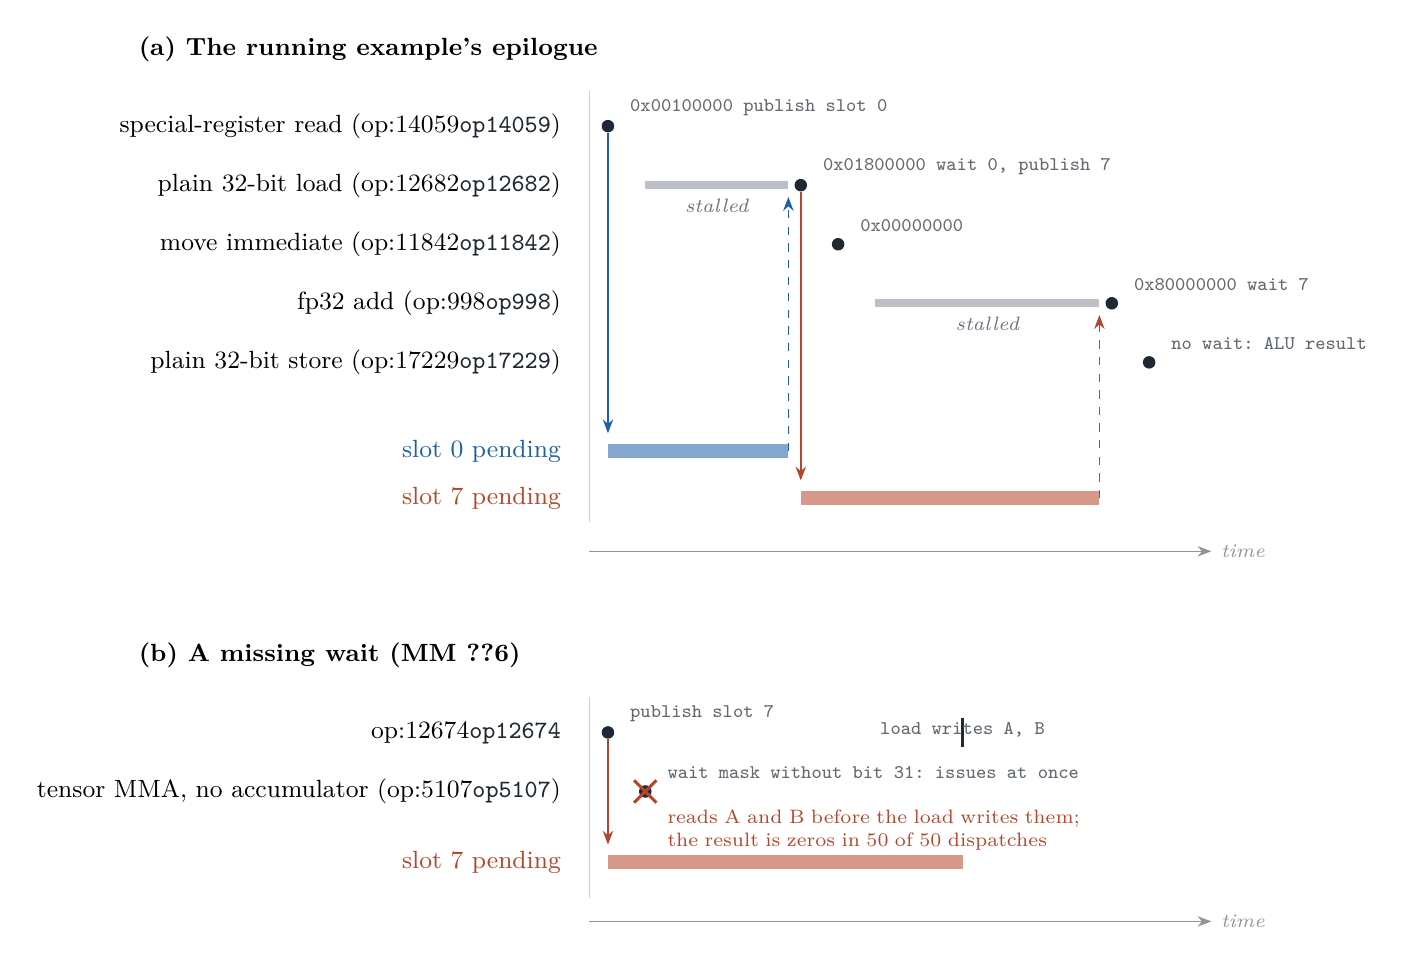
\begin{tikzpicture}[x=7.9mm, y=-7.5mm, font=\small,
    issue/.style={circle, fill=ink, inner sep=1.6pt},
    stall/.style={line width=3pt, color=apple!45},
    pend/.style={line width=5pt, color=#1!55},
    ins/.style={anchor=east, align=right, font=\small},
    ctl/.style={anchor=west, font=\scriptsize\ttfamily, text=ink!70}]
  \node[anchor=west, font=\small\bfseries] at (-7.4,-1.3) {(a) The running example's epilogue};
  % instruction rows
  \foreach \y/\n/\o in {0/special-register read/14059, 1/plain 32-bit load/12682,
      2/move immediate/11842, 3/fp32 add/998, 4/plain 32-bit store/17229}
    \node[ins] at (-0.3,\y) {\n\ (\opn{\o})};
  \draw[rule] (0,-0.6) -- (0,6.7);
  % slot lanes
  \node[ins, text=ours] at (-0.3,5.5) {slot 0 pending};
  \node[ins, text=native] at (-0.3,6.3) {slot 7 pending};
  \draw[pend=ours] (0.3,5.5) -- (3.2,5.5);
  \draw[pend=native] (3.4,6.3) -- (8.2,6.3);
  % issue points and stalls
  \node[issue] (i0) at (0.3,0) {};
  \draw[stall] (0.9,1) -- (3.2,1);  \node[issue] (i1) at (3.4,1) {};
  \node[issue] (i2) at (4.0,2) {};
  \draw[stall] (4.6,3) -- (8.2,3);  \node[issue] (i3) at (8.4,3) {};
  \node[issue] (i4) at (9.0,4) {};
  % publish and wait arrows
  \draw[->, ours, line width=0.6pt] (i0) -- (0.3,5.2);
  \draw[->, ours, line width=0.6pt, dashed] (3.2,5.5) -- (3.2,1.2);
  \draw[->, native, line width=0.6pt] (i1) -- (3.4,6.0);
  \draw[->, native, line width=0.6pt, dashed] (8.2,6.3) -- (8.2,3.2);
  % control words
  \node[ctl] at (0.5,-0.32) {0x00100000 publish slot 0};
  \node[ctl] at (3.6,0.68) {0x01800000 wait 0, publish 7};
  \node[ctl] at (4.2,1.68) {0x00000000};
  \node[ctl] at (8.6,2.68) {0x80000000 wait 7};
  \node[ctl] at (9.2,3.68) {no wait: ALU result};
  \node[font=\scriptsize\itshape, text=apple] at (2.05,1.35) {stalled};
  \node[font=\scriptsize\itshape, text=apple] at (6.4,3.35) {stalled};
  \draw[->, ink!50] (0,7.2) -- (10,7.2) node[right, font=\scriptsize\itshape] {time};

  \begin{scope}[yshift=-77mm]
  \node[anchor=west, font=\small\bfseries] at (-7.4,-1.3) {(b) A missing wait (MM~\mm{6})};
  \node[ins] at (-0.3,0) {\op{12674}};
  \node[ins] at (-0.3,1) {tensor MMA, no accumulator (\opn{5107})};
  \node[ins, text=native] at (-0.3,2.2) {slot 7 pending};
  \draw[rule] (0,-0.6) -- (0,2.8);
  \draw[pend=native] (0.3,2.2) -- (6.0,2.2);
  \node[issue] (j0) at (0.3,0) {};
  \node[issue] (j1) at (0.9,1) {};
  \draw[->, native, line width=0.6pt] (j0) -- (0.3,1.9);
  \node[ctl] at (0.5,-0.32) {publish slot 7};
  \node[ctl] at (1.1,0.68) {wait mask without bit 31: issues at once};
  \node[font=\scriptsize, text=native, align=left, anchor=north west, text width=52mm] at (1.1,1.15)
    {reads A and B before the load writes them; the result is zeros in 50 of 50 dispatches};
  \node[draw=native, cross out, line width=1.1pt, minimum size=7pt, inner sep=0pt] at (0.9,1) {};
  \draw[ink, line width=0.8pt] (6.0,-0.25) -- (6.0,0.25);
  \node[ctl, anchor=south] at (6.0,0.25) {load writes A, B};
  \draw[->, ink!50] (0,3.2) -- (10,3.2) node[right, font=\scriptsize\itshape] {time};
  \end{scope}
\end{tikzpicture}
\caption{Late values and their waits, as the control words specify them. A dot is an instruction's issue; grey is
an instruction held at issue by its wait mask; a coloured bar is a scoreboard slot that a producer has published and
that has not yet arrived. A dashed arrow is a slot's arrival releasing its waiter. The control words in (a) are read
from the running example's bytes (the low 32 bits of operand 1: bits 20--23 publish slot + 1, bits 24--31 are the
wait mask). Panel (b) is the measured missing-wait experiment. Only the ordering is measured: positions on the time
axis are schematic.}
\label{fig:scoreboard}
\end{figure}


The same field orders every late value (loads, atomics, imageblock reads, staging writes and special-register reads). The per-form carriers (general loads, the 128-bit vector load, tensor load, the tensor MMA's
scattered mask bits, the 12-byte ALU wait bits, \op{592}) are \cref{sec:scoreboard-publish-wait}'s table; this section
gives what they mean. Two carriers are not in that table: in 14-byte stores byte9{[}5{]} is slot 7 in this compiler's encoder
(\code{agxforge/g17/cc.py}), and for \op{12674} MM~\mm{6} called the whole field bits 20–27, which includes the
load's own wait mask; the fill slot is bits 20–23 alone. The general-load field is measured through executed consumers
(MM~\mm{25.115}, MM~\mm{25.121}; \code{tools/g17emu.py} \code{load\_hazards}), the staging-file slot only through the decoder (MM~\mm{25.120.1}).

The rule behind these comes from a decoder census: for 126 forms across 6,594 Apple programs, every instance's wait bits equal
exactly the slots its source registers are still pending on (\code{isa/g17-wait-mask-census.json}, MM~\mm{25.96}). It covers
stores: the \op{17256} uses every bit 24–31 (13,140 instances in a 314-object census, each one-hot
value present), which refuted an earlier "three-bit store limit" that was an encoder-table artifact (MM~\mm{6}). Tensor stores
are a separate class: all 876 \op{17257} and 118 \op{17258} instances carry a zero wait
byte, and the same-simdgroup MMA-to-tensor-store path is exact with no wait (measured, MM~\mm{6}).

\emph{Correction:} the 8-byte \op{17229} does carry wait bits (15 corpus instances match their pending
slots, \code{isa/g17-wait-mask-census.json}; Apple's \code{tex2d-read} carries 0x1000010 on one, MM~\mm{25.146}). The "no wait bit" note
in \code{agxforge/g17/cc.py} describes this compiler's encoder, which has no carrier for them (\cref{app:a}).

Which consumers need a wait has been measured:

\begin{itemize}
\item \emph{Not needed:} ordinary ALU to ALU. 52 of 52 ordered adjacent pairs of ordinary ALU instructions read the previous
  result bit-exactly with no wait (MM~\mm{25.90}, MM~\mm{6}).
\item \emph{Needed:} loads, imageblock reads, vector-load lanes, the packed half2 load, atomic returns, texture fetches and staging
  writes. "Needed" applies to every consumer kind: an indirect load whose index is a loaded value read index 0 on every
  lane (1 of 32 right) until its operand 1 also named slot 7 (32 of 32; MM~\mm{25.104}, MM~\mm{25.90}); \code{simd\_shuffle\_xor} and
  \code{simd\_broadcast} reading a loaded value directly read it before it arrived (MM~\mm{25.90}); \op{11190}, \op{9986}, \op{14047} and \op{590} do not interlock on a load
  (MM~\mm{25.133}); a store takes its value register at issue (MM~\mm{25.96}).
\item \emph{Special-register reads:} \op{14059} publishes a slot and Apple's compiler always waits on it,
  but a slot-0 read is readable at distance 0 with no wait, and the wait has no measurable cost (measured, MM~\mm{25.117}, MM~\mm{25.121}; the probe and the counts are \cref{sec:read-latency-whether}).
\item \emph{Open:} whether an ALU consumer of an MMA result is interlocked. One ALU consumer placed directly after an MMA carried
  no wait and still read the result; no measured pair had an MMA producer (MM~\mm{6}, MM~\mm{25.90}).
\end{itemize}

An unwaited consumer could read arbitrary data, the late value if it happened to arrive in time, or the register's
previous contents. To tell these apart the producer's destination was pre-set. With a poison in it, the
four non-interlocking unary forms returned exactly op(poison) on every lane; with a fresh register they returned op(0); a
negative control, an add with its load-wait bit cleared, read the poison on 1,024 of 1,024 lanes, so the instrument can
see a race (measured, MM~\mm{25.133}). The unwaited consumer reads the previous contents, which is why most observed
failures read 0 and why detecting them takes a sentinel or poison value; a zero-filled buffer cannot show them. Added
distance does not help; an atomic whose return was published on a slot its consumer did not name returned 0 with
64 independent instructions in between (below).

\textbf{Worked example: an atomic return published on the wrong slot} (decoded, then executed on hardware; MM~\mm{25.115},
\code{docs/g17-first-dispatch-trials.md}). This compiler's residency probe counts arrivals with \op{10094} and reads the returned old value. At S = 256 simdgroups every arrival read 1 (a returned 0, plus
one) while the departure maximum was 256. Of the two explanations that fit, the one first recorded, and later withdrawn, was that
simultaneous same-address atomics combine and each requester sees the pre-combine value. The other is that the consumer
read the register before the return arrived. The decoded bytes favoured the second. Marking the atomic's result late
gave its consumer, \op{10279}, this compiler's load-use wait, mask 0b10000000, slot 7, because this
compiler's loads fill slot 7. But the atomic's operand 1 bits 20–23 were 1: it filled slot 0, copied from Apple's
witnesses, where Apple's first consumer waits on bit 24 (120 of 120 corpus instances). The consumer waited on a slot the
atomic never touched. At larger S arrivals had agreed with departures, which had been read as the wait working; in fact
the arrivals were staggered enough that each return landed before its consumer read it. The discriminating run changes only the slot: publishing the atomic on slot 7
(the two programs differ in four bytes) gave an arrival maximum of 256, equal to the departure maximum, 3 of 3, while the
slot-0 arm read 1. Combining would not depend on which slot the return is published on. Below Metal, the per-lane form behaved the same way: a 12-byte \op{10090}
publishing on slot 0 (operand 1 0x80100000) updated all 64 cells correctly and returned 0 to every lane, still 0 with 64
independent two-byte moves inserted before the consumer; changing two atomic bytes to publish on slot 7 (operand 1
0x80800000) returned all 64 old values. In both cases the fix was to name the producer's actual slot in the consumer's
mask.

Rules for choosing and reusing slots:

\begin{itemize}
\item Past eight groups the slot sequence Apple's compiler assigns is scheduler-chosen (twelve loads got 8, 1, 2, 3, 4, 4, 4,
  4, 7, 7, 6, 5 in decoded values), so an emitter should use an explicit rule, such as K-step k in slot k mod 8; this
  compiler's K = 256 lowerings use slot k mod 7, exact in 3 of 3 cases (MM~\mm{6}, \code{tools/tensorops-model/scoreboard-store-census.json}).
\item Reusing a slot after its named consumer has waited is safe (measured); reuse before that consumer is unmeasured and
  forbidden (MM~\mm{0.14}, MM~\mm{6}).
\item Not every slot works for every producer. Loads and atomic returns work on slot 7 (measured), but a special-register read
  publishing on slot 7 stored nothing, waited or not, recorded and not explained (measured, MM~\mm{25.121}; \cref{sec:read-latency-whether}). Use a
  slot that has been measured for that producer kind.
\item Atomic return slots (contradiction resolved by scope): the glossary's "the return fills scoreboard slot 7" for the
  uniform-address atomic and \op{11765} describes this compiler's emission. Apple's corpus fills slots 0
  and 1, and every first consumer waits on exactly that slot (25 of 25 for the uniform atomic, MM~\mm{25.115}). Slot 7 is this compiler's convention,
  checked on hardware; Apple's corpus does not use it, and the hardware does not require it.
\end{itemize}

The release lifetime (16) is destructive and per lane (\cref{ch:register-file}): a store naming one
register as both value and index, with the index slot releasing it, stores 0 (measured, MM~\mm{25.117}), and an instruction no
lane executes releases nothing (MM~\mm{25.95}).

\section{Barriers and fences}\label{sec:barriers-fences}

The \op{447} is one six-byte instruction with scheduling class 3, MayStore, NotDuplicable and side effects.
Only operand 1, the scope immediate, changes with the Metal barrier (\cref{tab:barrier-scopes}; Apple's compiler emits,
\code{isa/g17-barrier-scopes.txt}).

\begin{longtable}{@{}lll@{}}
\caption{Metal threadgroup barriers with the bytes and scope immediate Apple's compiler emits for each.}\label{tab:barrier-scopes}\\
\toprule
Metal barrier & Bytes & Scope \\
\midrule
\endfirsthead
\tablecontinued{3}
\toprule
Metal barrier & Bytes & Scope \\
\midrule
\endhead
\code{threadgroup\_barrier(mem\_none)} & \code{075100060000} & 20 \\
\code{threadgroup\_barrier(mem\_device)} & \code{0f6900060000} & 154 \\
\code{threadgroup\_barrier(mem\_threadgroup)} & \code{275100060000} & 276 \\
\code{threadgroup\_barrier(mem\_texture)} & \code{876700060000} & 1144 \\
\code{threadgroup\_barrier(mem\_threadgroup\_imageblock)} & \code{475100060000} & 532 \\
\bottomrule
\end{longtable}

\code{mem\_threadgroup | mem\_device} emits two barriers, one per flag; \code{simdgroup\_barrier} emits nothing at all
(Apple's compiler emits, \code{isa/g17-atomic-semantics.json} barriers). Scopes 16, 528 and 1138 substituted for 276 each
carried a threadgroup-memory round trip (measured, the threadgroup-barrier notes in \code{tools/g17emu.py}).

Between simdgroups a threadgroup barrier is mandatory (measured, MM~\mm{14}, MM~\mm{17} rule 7). With no barrier, and with
\code{air.simdgroup.barrier} alone (which emits no instruction), a cross-simdgroup hand-off was wrong in 12 of 12 trials and
the consumer read exactly the buffer's pre-write state, a race rather than garbage. Every workgroup-barrier variant
(execution-only, threadgroup memory, device memory, both) was correct in 12 of 12. Below Metal, threadgroup store,
barrier and load exchanged values between the two simdgroups of a 64-thread group, and also in a half-full 32-thread
second group (measured, \code{docs/g17-first-dispatch-trials.md}; other partial sizes and inactive-lane accesses untested).

MM~\mm{14} and the emulator treat device-memory ordering between simdgroups differently without conflicting. MM~\mm{14} observed that the execution-only barrier (scope 20) sufficed, and says so as "an observation about this chip, not a guarantee". The
emulator's race check (MM~\mm{25.197}) orders threadgroup memory across every threadgroup barrier but device memory only across scope 154,
a conservative choice that no measurement forced. Scope 276 (or any threadgroup barrier scope) is safe for threadgroup
memory between simdgroups, and scope 154 for device memory between simdgroups of one threadgroup. Code must not rely on scope 20 to
order memory, on any threadgroup barrier to order anything across threadgroups, or on \code{simdgroup\_barrier} to do anything.

\textbf{Worked example: threadgroup barrier against device fence} (executed on hardware, MM~\mm{25.140.5}). Every threadgroup
writes a marker, crosses a barrier, and counts itself with \op{10094} on its rank-0
written buffer; the last threadgroup to arrive sums all markers. With the barrier at scope 154 the count was a perfect
permutation, yet the last threadgroup read stale markers: it summed 1,560 of 2,080 at 64 threadgroups and 123,408 of
131,328 at 512, differing by round. Apple's compiler, given
\code{atomic\_thread\_fence(mem\_device, seq\_cst, thread\_scope\_device)}, emits \op{14156}, operands (0, 186), six
bytes \code{0f2b00060000}, no registers, and places one after the stores and one again inside the last threadgroup's region;
the loads stay ordinary. With those two fences both sums were exact. This compiler now emits those bytes, read back
through Apple's decoder. A fused attention merge built on the pattern was bit-exact at q0 = 0, 5, 128 and 271 over five
rounds each, with NaN-poisoned rows (costs are \cref{ch:performance}'s).

The imageblock barrier is the threadgroup barrier at scope 532 (\cref{sec:imageblock-per-core-tile}). The emulator admits it only for one simdgroup in
lockstep; more than one simdgroup was never witnessed (MM~\mm{25.145.2}). A barrier inside an exec-mask region is not modelled
there either (\code{tools/g17emu.py}).

Encoder-level barriers come from a static read of the AGX user driver (decoder, MM~\mm{25.141.20}); their costs are measured
in \cref{ch:performance}.

\begin{itemize}
\item A serial compute encoder emits a barrier token after every dispatch. A concurrent encoder emits one only where
  \code{memoryBarrierWithScope:} asks; in a serial encoder that call only posts a notification. For a chain where every
  dispatch depends on the last, both emit the same tokens.
\item The token is one 32-bit command word, 0x60000160, OR 0x1000 when a pending flag is set; with its boolean arguments it
  ORs 0x400 or appends 0x60000502, both of unknown function. Its cost is the GPU draining at the token.
\item Hazard tracking never enters the per-dispatch path: tracked and untracked buffers encode identically inside an encoder.
  Consecutive compute encoders in one command buffer are merged, with an unconditional barrier after a concurrent one.
\item Measurements agree with this: tracked buffers with one serial encoder per token beat untracked buffers ordered by an
  \code{MTLSharedEvent} between command buffers, and untracked buffers without ordering race (MM~\mm{0.15}).
\end{itemize}

Below Metal, two dependent Submits on one queue (the second reading the first's output) computed exactly, also with a
program switch between them; and one Submit carrying two or three command records, each running a per-lane \code{+7}
read-modify-write on the same words, left 14 and 21 in every lane, so each record saw the previous record's result
(measured, \code{docs/g17-first-dispatch-trials.md}, "Dependent two-stage pure GPU pipeline" and "One to three dependent GPU
computations in one Submit"). The ordering of other command shapes, and whether records can overlap, is unmeasured.

\section{Atomics}\label{sec:atomics}

In the decoder (\code{isa/g17-atomic-family.toml}), 208 opcodes share the scheduling class of \op{10094} and flags
(classes 286 and 287 with flags 0x402002400 for device scope, class 329 with 0x402002800 for threadgroup scope) and one
operand skeleton, \code{[dest] imm imm [address] imm [index] imm imm imm [value] imm}, with parts present or absent. Five occur
in the corpus; 29 are reachable from one encoding of it by bit flips. The other 179 were never produced by single-bit
walks to saturation, 132,240 two-bit mutations, 1,365,504 three-bit mutations or 800,000 random encodings; the boundary is
width (a bounded negative). Its structural bits: byte4{[}0{]} returns old (to \op{10022}); byte4{[}1{]} selects a threadgroup GPR16 address over a device register pair (\op{11769}, no glossary entry);
byte5{[}2{]} selects an index register (\op{10090}); byte6{[}2{]} leaves the family.
\Cref{tab:atomic-forms} lists the forms this chapter uses.

\begin{xltabular}{\linewidth}{@{}>{\hsize=1.18\hsize}Xl>{\hsize=0.85\hsize}XX@{}}
\caption{Atomic forms by address kind.}\label{tab:atomic-forms}\\
\toprule
Glossary name & Opcode & Address & Standing \\
\midrule
\endfirsthead
\tablecontinued{4}
\toprule
Glossary name & Opcode & Address & Standing \\
\midrule
\endhead
uniform-address atomic, returning old & \opn{10094} & device, uniform, byte offset in operand 6 & measured (below Metal, all operations below; MM~\mm{25.140.3}) \\
uniform-address compare-exchange, returning & \opn{10095} & device, uniform & measured (below Metal) \\
uniform-address no-return atomic, 32-bit & \opn{10022} & device, uniform & Apple's compiler emits \\
uniform-address no-return compare-exchange & \opn{10023} & device, uniform & Apple's compiler emits \\
per-lane-address atomic, returning & \opn{10090} & device, base + index register & measured (below Metal) \\
per-lane-address compare-exchange, returning & \opn{10091} & device, base + index register & measured (below Metal) \\
per-lane-address no-return atomic & \opn{10019} & device, per lane & Apple's compiler emits \\
64-bit no-return atomic, max/min & \opn{9996} & device & Apple's compiler emits \\
threadgroup atomic, returning old & \opn{11765} & threadgroup & measured (MM~\mm{25.115}) \\
threadgroup atomic, no return & \opn{11701} & threadgroup & measured (glossary) \\
\bottomrule
\end{xltabular}

Below, "the uniform atomic" means \op{10094} and "the per-lane atomic"
\op{10090}. "Uniform-address" describes the address, not the issue: the uniform atomic
executes once per active lane, so 32 lanes add 32 and receive 32 distinct old values (measured, MM~\mm{25.140.3}). Its operand 6 is the address's byte offset: values 4, 8 and 16
moved the cell by 1, 2 and 4 words. \emph{Correction:} earlier claims called operand 6 a source lifetime ("16 writes nothing");
the probe had watched the wrong word (MM~\mm{25.140.3}).

The operation is a four-bit field, named by the decoder's operation operand. The decoder prints operand 2 as
0x40200 + code, so every executed operation has an unambiguous name: 262656 + code. For the uniform atomic the four bits
are byte4{[}5{]}, byte5{[}3{]}, byte6{[}3{]} and byte7{[}7{]}; \cref{tab:atomic-operation-codes} reproduces all ten encodings Apple's compiler emits for
\code{atomic\_fetch\_\{add,sub,and,or,min,max\}} (both signednesses), \code{atomic\_exchange} and \code{atomic\_fetch\_xor} (decoder plus
Apple's compiler, \code{isa/g17-atomic-family.toml}) and gives the uniform atomic's shortest length for each code.

\begin{xltabular}{\linewidth}{@{}l>{\hsize=1.47\hsize}X>{\hsize=0.74\hsize}X>{\hsize=0.79\hsize}X@{}}
\caption{Atomic operation codes, with the operand value the decoder prints, the uniform form's shortest length in bytes and
whether it has executed below Metal.}\label{tab:atomic-operation-codes}\\
\toprule
Code (operand) & Operation & Shortest length, uniform form & Executed below Metal, uniform form \\
\midrule
\endfirsthead
\tablecontinued{4}
\toprule
Code (operand) & Operation & Shortest length, uniform form & Executed below Metal, uniform form \\
\midrule
\endhead
0 (262656) & add & 10 & yes, returns consumed \\
1 (262657) & sub & 12 & yes \\
2 (262658) & exchange & 12 & yes \\
3 (262659) & compare-exchange: selects \op{10095} & 10 & yes \\
4 (262660) & unsigned min & 12 & yes \\
5 (262661) & signed min & 10 & yes \\
6 (262662) & unsigned max & 12 & yes \\
7 (262663) & signed max & 10 & yes \\
8 (262664) & and & 10 & yes \\
9 (262665) & or & 10 & yes \\
10 (262666) & xor & 12 & yes \\
12 (262668) & fp32 add, emitted by no tested Metal builtin & 10 & yes \\
\bottomrule
\end{xltabular}

Four combinations do not decode. The same operand values name the per-lane operations, but the bits carrying them differ
by form and length: in the 12-byte per-lane atomic the fourth bit is byte11{[}4{]}, and a decoder sweep of that form maps the
assembler's three-bit operation with byte11{[}4{]} set and clear onto these codes (\code{docs/g17-first-dispatch-trials.md},
"Per-lane AND old-value return"). An authored "OR" with byte11{[}4{]} set executed exchange, updating every cell to the new
value; clearing that one bit gave operand 262665 and OR (measured). \emph{Correction:} the "eight unassigned raw operation
codes" of \code{isa/g17-atomic-semantics.json} were read off one witness's field placement and are retracted
(\code{isa/g17-atomic-family.toml}; \cref{app:a}); a census of unassigned codes must be made per form.

The following semantics were measured below Metal (\code{docs/g17-first-dispatch-trials.md}; \code{isa/g17-atomic-family.toml}),
all in relaxed order, single dispatch, each case in two fresh processes with output guards.

\begin{itemize}
\item \emph{Atomicity.} 64 lanes adding to one cell left exactly the sum (5 to 69 with +1; 5 to 2085 with lane i adding i + 1), and
  every lane received a distinct old value; with lane-varying addends the returned values form a unique chain through all
  64 lanes. Two simdgroups' elected lanes on one uniform atomic received non-overlapping intervals (5–36 and 37–68).
\item \emph{Integer operations} behave as named, including 32-bit modular sub (5 - 32 - 32 = 4294967237), signed against unsigned
  extrema on 0xFFFFFFFF and 0x80000000, and exchange.
\item \emph{Compare-exchange.} The register tuple is (desired, expected), established from the compiler's witness; matched and
  failed compares both returned the old value.
\item \emph{fp32 add (code 12)}, uniform and per-lane: 1.0f + 1.0f + 1.0f gave returned values 1.0f, 2.0f and final 3.0f; 64
  per-lane updates of 1.0f from 1.0f reached 65.0f and returned 1.0f through 64.0f once each. Each update rounds to
  nearest even: half-ULP ties left an even mantissa unchanged and moved an odd one up once (0x3F800001 to 0x3F800002) and
  no further. Subnormal inputs, operands and results flush to zero. A quiet NaN seed 0x7FC12345 was returned raw to its
  first caller and then stored as canonical 0x7FC00000; −0 plus +0 returned −0 and stored +0; infinities were preserved.
  Signaling NaNs and other payloads are untested.
\end{itemize}

Atomics have been run only on the rank-0 buffer, through Metal and below it; this compiler refuses an
atomic whose identity base and binding rank disagree (open, \code{agxforge/g17/cc.py}; MM~\mm{25.140.3}). Threadgroup atomics need a
threadgroup region, which only an ordinary threadgroup load or store provisions (\cref{sec:threadgroup-memory}).

Atomic return values are late; the fill slot is operand 1 bits 20–23 minus 1, and slot choice is in \cref{sec:scoreboard}. The 10-byte uniform atomic also releases its value: operand 9 is the value's lifetime and only 16 is
representable, so a second atomic sharing a constant read 0 (A{[}0{]} = 0 against 24; measured by this compiler's fuzzer,
MM~\mm{25.144.6}, \code{agxforge/g17/cc.py}); a value read again must be copied first.

Validation with a consumed return, by form:

\begin{itemize}
\item The uniform atomic, below Metal: all eleven of its operations in \cref{tab:atomic-operation-codes} (every code except 3), each under two-group
  contention with the returned old value consumed; \op{10095} at match and
  mismatch. Through Metal, add (the residency probe, MM~\mm{25.115})
  and the compiler's wave-broadcast program (\code{agxforge/g17/cc.py}).
\item The per-lane atomic, below Metal: update-only for add, and, or, sub, xor, signed and unsigned min and max, exchange and
  fp32 add; returns through slot 7 for add (also contended, both fixed and lane-varying addends), and, or, sub, xor and
  fp32 add (also contended, half-ULP and NaN cases). Compiler-generated 12-byte programs for add, and, or, sub and xor
  passed with a direct indexed-store consumer, plus an ordinary add consumer for add and xor.
\item \Op{10091}: hand-authored slot-7 return (one matching and 63 failing compares), then
  compiler-generated programs at index placements R0, R1, R5, R7 and R12 (ten Submits); other placements are decode-checked
  predictions, and placement 13 is refused.
\item \Op{11765}: dispatched through Metal with its return consumed; its \op{11667} consumer had read both returns with an empty wait mask until fixed, where Apple waits 10 of 10 (MM~\mm{25.115}).
\item Not validated: per-lane min and max returns, unsigned long-form returns, other consumer shapes (refused by this
  compiler), 64-bit atomics (\op{9996}, compiled only), and any atomic on a buffer other
  than rank 0.
\end{itemize}

An atomic does not order other memory. The count in \cref{sec:barriers-fences}'s worked example was exact while the data it
guarded was stale. Ordering of ordinary stores through an atomic needs \op{14156}. The emulator does not
track atomics in its race check and does not model acquire or release through atomics or the fence, so it refuses any
program that synchronises threadgroups through an atomic counter (MM~\mm{25.197}).

\section{Ordering by scope}\label{sec:ordering-across-lanes}

\subsection*{Lanes of one simdgroup}

\begin{itemize}
\item Program order holds on one scoreboard: a store followed by a load in one simdgroup needs no fence, as two separately
  generated bodies joined at a shared buffer showed, including a cross-lane stress where each lane read another lane's
  write (measured, MM~\mm{13}). Late values still need the consumer's wait.
\item Same-address stores with \op{17229}: the lowest active lane wins, by lane and not by value (all
  lanes: lane 0; lanes 0–15 under an exec region: lane 0; odd lanes: lane 1; reversed values: lane 0; five runs each;
  measured, MM~\mm{25.145.4}, \code{isa/g17-execution-storewinner-results.json}). Across simdgroups the winner is unmeasured.
\item Registers never cross a simdgroup: a cross-simdgroup \code{simd\_shuffle} returns the caller's own value, 256 of 256
  (measured, MM~\mm{14}).
\end{itemize}

\subsection*{Simdgroups of one threadgroup}

Simdgroups are ordered only across a \op{447} (\cref{sec:barriers-fences}). Same-value writes by several simdgroups are
harmless by construction (no schedule changes the bytes), and shipped code relies on that: the fused attention appends a
new K/V row from every simdgroup of every threadgroup and each reads its own copy back (modelling rule, MM~\mm{25.197}).

\subsection*{Threadgroups of one dispatch}

MM~\mm{0.14}'s map says "cross-threadgroup handoff requires a
dispatch boundary". It was written about tensor fragment hand-offs before any in-dispatch mechanism had been measured, and
MM~\mm{25.140.5} and MM~\mm{25.141.1} have since measured two, so the statement is superseded in part:

\begin{itemize}
\item \emph{Visibility.} Device stores from one threadgroup are visible to another in the same dispatch after \op{14156}
  on the writer side and again on the reader side (measured for the last-threadgroup pattern, MM~\mm{25.140.5}). A threadgroup
  barrier at any scope does not provide it (measured, same section).
\item \emph{Ordering.} An atomic count decides who is last; atomicity is measured (\cref{sec:atomics}). Without the fences the count can be
  right and the data stale.
\item \emph{Forward progress.} The last-threadgroup pattern needs none, because no threadgroup waits: whoever counts last does the
  follow-on work. Any pattern that waits needs the producer resident: in the forward-progress probe the first resident
  wave spun to its cap before the producer, dispatched last, ran at all (measured, MM~\mm{25.141.1}; the grid sizes and counts
  are \cref{sec:forward-progress-in-order}). In the tested configurations a grid barrier among resident threadgroups, fenced and capped, kept
  totals exact in every run and never reached its cap (measured, MM~\mm{25.141.1}). No progress guarantee follows
  beyond those configurations, and the barrier costs more than the dispatch boundary it replaces (\cref{sec:dispatch-encoder-command-buffer}).
\end{itemize}

\emph{Correction:} "cross-threadgroup handoff requires a dispatch boundary" (MM~\mm{0.14}) is the safe default, not a hardware
limit; fenced atomic patterns work within one dispatch under the conditions above.

\textbf{Residency of large threadgroups (unresolved).} For 1,024-thread threadgroups the forward-progress probe implies at least
10 co-resident per core and the driver formula gives 3 (MM~\mm{25.141.1}, MM~\mm{25.141.20}); no residency count may be assumed, and
a spin-waiting grid of them must not be sized from either number (\cref{sec:residency-occupancy-rules}, rule 5).

\subsection*{Dispatches}

Dispatch order and the absence of observed preemption are as stated at the head of the chapter
(\cref{sec:forward-progress-in-order}). A serial encoder places
a barrier token after every dispatch; a concurrent encoder lets a dependent kernel start early, but its threadgroups queue
behind all of the producer's, so only the producer's last-wave tail overlaps (measured, MM~\mm{25.141.1}; costs \cref{ch:performance}).
The GPU's L2 is not coherent with CPU stores: a recently read line of a write-combined buffer the CPU updates reads stale
(measured, MM~\mm{0.15}). A submitted command buffer outlives its host process (\cref{sec:faults-hangs-recovery}).

\subsection*{Safe ordering patterns}

\begin{enumerate}
\def\labelenumi{\arabic{enumi}.}
\item Within a simdgroup: program order, plus a wait on the producer's actual slot for every late value. Never rely on
  distance.
\item Between simdgroups: one threadgroup barrier at a scope covering the memory used (276 for threadgroup memory, 154 for
  device memory).
\item Between threadgroups in one dispatch: a device fence after the stores, an atomic count, a device fence again before
  reading; or a dispatch boundary. Never a threadgroup barrier alone.
\item Waiting on another threadgroup only when every participant fits in measured resident capacity at the kernel's own
  register and threadgroup-memory use, with capped spins and work pulled from an atomic queue (MM~\mm{17} rule 40); never spin
  on a producer that may not be resident.
\item Between dispatches: a serial encoder, or a concurrent encoder with barriers at every true dependency.
\end{enumerate}

\textbf{Not known.} MMA-to-ALU interlock; the cross-simdgroup winner of same-address stores; whether an execution-only
barrier orders device memory by design; why a special-register read on slot 7 stores nothing; per-lane min, max and
unsigned long-form atomic returns; atomics beyond rank 0; 64-bit atomics on hardware; acquire and release semantics in
general (only the fence-count-fence pattern is measured); the function of the barrier-token variants 0x400 and 0x60000502;
the residency count for 1,024-thread threadgroups.

\textbf{Evidence.} MM~\mm{0.8}, MM~\mm{0.14}, MM~\mm{0.15}, MM~\mm{6}, MM~\mm{13}, MM~\mm{14}, MM~\mm{17} rules 4, 7, 35 and 40, MM~\mm{25.90}, MM~\mm{25.95}, MM~\mm{25.96},
MM~\mm{25.104}, MM~\mm{25.115}, MM~\mm{25.117}, MM~\mm{25.120.1}, MM~\mm{25.121}, MM~\mm{25.133}, MM~\mm{25.140.3}, MM~\mm{25.140.5}, MM~\mm{25.141.1}, MM~\mm{25.141.20},
MM~\mm{25.144.6}, MM~\mm{25.145.2}, MM~\mm{25.145.4}, MM~\mm{25.146}, MM~\mm{25.197}; \code{isa/g17-barrier-scopes.txt}, \code{isa/g17-atomic-family.toml},
\code{isa/g17-atomic-semantics.json}, \code{isa/g17-wait-mask-census.json}, \code{isa/g17-execution-storewinner-results.json},
\code{docs/g17-first-dispatch-trials.md}, \code{agxforge/g17/cc.py}, \code{tools/g17emu.py},
\code{tools/tensorops-model/scoreboard-store-census.json}.

\chapter{The tensor unit}\label{ch:tensor-unit}

The tensor unit (Apple's "neural accelerator") performs one 16 × 16 × 16 matrix multiply-accumulate
per instruction, \code{D = C + A.B} or \code{D = A.B}: 4,096 multiply-accumulates and 8,192 floating-point operations per issue,
with one tensor-issue slot per SIMD and four per core (measured, MM~\mm{0.1}, MM~\mm{8}; a logical resource model, not a
floorplan). It is distinct from the older 8 × 8 simdgroup-matrix engine (\cref{sec:legacy-simdgroup-matrix-engine}) and from the Apple Neural
Engine, which this reference does not cover.

The instruction's operands are register tuples spread across the 32 lanes of one simdgroup, and no unit between
memory and those registers handles them as a matrix. Most of the rules summarised here follow from that.

\begin{itemize}
\item A 16 × 16 tile has 256 elements; each lane holds 8 of them in fixed slots. The map is
  closed-form (\cref{sec:fragment-layouts}), and it is produced only by per-lane address arithmetic in ordinary ALU code; a "tensor
  load" is a gather, and there is no tile-layout unit (\cref{sec:tensor-memory-path}).
\item A lane's 8 elements occupy an aligned tuple: 2 registers for int8, 4 for 16-bit
  types, 8 for fp32 operands and for every accumulator. The 10-byte instruction names each tuple in units of its width,
  attaches a type code to A and B (a transpose adds 32 to it) and a lifetime modifier to every register (\cref{sec:instruction-family,sec:modifiers-keep-flag}). A transpose changes how the registers are read and moves no data.
\item For half inputs, the case the rule was fitted on, the sixteen products of each output are exact
  and are reduced by a fixed tree with an fp32 rounding at every node, the accumulator entering first
  (\cref{sec:arithmetic-semantics-supported}); bfloat and truncated-fp32 inputs are recorded only at single points. fp32
  operands are truncated to 10 fraction bits on the way in; int8 sums wrap or, with one bit, saturate once per issue.
\item The MMA waits for its operand loads only through an 8-bit mask naming the scoreboard slots those loads
  fill; a slot it does not name is not waited on, and in every measured case the MMA then read zeros, with no error
  (\cref{sec:ordering-enable}).
\item Because D is eight ordinary registers per lane in the same lane map, it can be the next MMA's C, A or B with
  no store (\cref{sec:chaining-feed-modes}). What the next MMA then computes depends on how the producing kernel labeled its rows, not on
  the instruction: the same hand-off computes the logical \code{A2 . D} in this compiler's measured kernels and a row-rotated product
  in Apple-compiled \code{simdgroup\_matrix} code (\cref{sec:coordinate-systems}).
\item None of the ten admitted forms takes an fp8, int4 or fp4 operand, applies a
  block scale or accumulates in 16 bits, and no cross-simdgroup register path was found; in every route tested these
  are built from ordinary instructions around the ten forms (\cref{sec:across-simdgroups,sec:quantized-formats}).
  int8 and uint8 are native.
\end{itemize}

Four of these replace earlier readings; the corrections are recorded where each is measured. The "two layouts" are
one map and a row rotation (\cref{sec:fragment-layouts}); the reduction tree is now fixed by 1,680 discriminating stimuli
(\cref{sec:arithmetic-semantics-supported}); the "result ring" is a wait mask (\cref{sec:ordering-enable}); and the feed
relabelings come from the way Apple's kernels pack their tiles (\cref{sec:chaining-feed-modes}).

\leadhead{Notation.}

\begin{itemize}
\item \textbf{MMA}: one tensor multiply-accumulate instruction. "With-C" forms read an accumulator C; "no-C" (from-zero) forms
  do not.
\item \textbf{The 16-bit MMA}: \op{5106}, the form most measurements use; the other
  nine forms are named in full (\cref{sec:instruction-family}).
\item \textbf{Tile}: a 16 × 16 matrix. A is M × K (16 × 16), B is K × N, C and D are M × N. Larger GEMMs are grids of tiles.
\item \textbf{Fragment}: the part of one tile held by one lane. Every lane holds 8 logical elements of a tile, numbered by a
  \textbf{slot} \code{j} in 0..7; lane \code{l} is 0..31 (SR130, the lane index within the simdgroup, \cref{ch:special-registers}).
\item \textbf{Tuple}: the aligned group of consecutive registers holding a fragment: 2 registers for int8, 4 for half or
  bfloat, 8 for fp32 operands and for every accumulator. A tuple's base register must be a multiple of its width.
\item \textbf{Accumulator group}: an 8-register fp32 or int32 tuple (C and D). Legal bases are R0, R8, \dots{}, R112 (15 groups).
\item \textbf{Modifier}: the immediate that follows every register operand in the decoded form, carrying the operand's
  lifetime bits (release and keep). The general rule is in \cref{ch:register-file}, the tensor-specific use in \cref{sec:modifiers-keep-flag}.
\item \textbf{Feed}: using one MMA's D as a later MMA's A, B or C without a store.
\item \textbf{Memory bridge}: storing D to row-major memory with a tensor store and reloading it with a tensor load.
\item \code{rotl1(x)} / \code{rotr1(x)}: rotate a four-bit row index left or right by one bit.
\item \code{RNE32(x)}: round x to fp32, nearest-even.
\item "pos" layout and "pos\_b" layout: the two (lane, slot) maps of \cref{sec:fragment-layouts}.
\item \textbf{Silent}: a violation produces wrong or zero results with no error from compiler, driver or API.
\item The statement kinds are those of \cref{sec:read-this-document}, with \emph{decoder} written \emph{decoder only}.
\end{itemize}

Every result in the chapter is from one M5 Pro (H17s, 20 cores) and one toolchain; the Metal-path evidence files behind
most of it do not record the OS build (\cref{sec:measured-part-software}; MM~\mm{0.1}, MM~\mm{20}).

\section{Access through Metal}\label{sec:it-reached}

Metal 4's TensorOps API reaches the unit through four layers, and only the last is a matrix instruction (Apple's
compiler emits, MM~\mm{1}):

\begin{enumerate}
\def\labelenumi{\arabic{enumi}.}
\item \code{mpp::tensor\_ops::matmul2d<descriptor, execution\_simdgroups<N>>::run} is header code. It calls \code{extern "C"} symbols
  named \code{\_\_tensorops\_impl\_matmul2d\_op\_run\_<left>\_<right>\_<dest>[\_v2]}, declared in the \code{air.externally\_defined}
  section, so a TensorOps kernel's AIR holds only a call to one of these symbols.
\item The symbols resolve at native compile time from
  \code{MetalPerformancePrimitives.framework/Resources/libTensorOps.rtlib}, an ar archive of 1,970 air64\_v28 bitcode
  members, 1,475 of them \code{matmul2d\_op\_run\_*}.
\item Inside the library, \code{air.supports\_family(i32 1010)} (\code{MTLGPUFamilyApple10}: M5 and A19 Pro) selects
  \code{air.simdgroup\_matrix\_16x16x16\_multiply\_accumulate}; family 1009 selects the older
  \code{air.simdgroup\_matrix\_8x8\_multiply\_accumulate}. Which engine a TensorOps kernel uses is decided by this
  predicate in Apple's library.
\item The 16 × 16 × 16 intrinsic lowers to one native instruction, \op{5106}, or
  a sibling from \cref{sec:instruction-family}.
\end{enumerate}

The AIR intrinsic surface is
\code{16x16x16\_multiply\_accumulate.f.f.v8f32.\{v8f16|v8bf16|v8f32\}.\{v8f16|v8bf16|v8f32\}.v8f32} (nine A/B combinations, fp32
accumulator only) plus the integer widening form \code{.\{s|u\}.\{s|u\}.v8i32.v8i8.v8i8.v8i32}. A fragment is a per-lane
\code{<8 x T>} value (Apple's compiler emits, MM~\mm{1}). Hand-written AIR reaches the intrinsic directly, which is how the
saturating int8 form, fp8 and the scaled spelling were reached (\cref{sec:instruction-family,sec:quantized-formats}).

\code{relaxed\_precision} selects the mixed float forms. Without it, the mixed float intrinsics fall to the legacy
datapath with a different layout; with it they reach \op{5098}, \op{5100} and \op{5104}. It is inert for forms already
native (Apple's compiler emits, measured, MM~\mm{17} rule 29). \emph{Correction:} the reading that the fp32-A forms, with and
without an accumulator (the latter \op{5101}), are never compiler-emitted
(MM~\mm{19}) is withdrawn; they are emitted under \code{relaxed\_precision}.

Apple's library body changes with the simdgroup count (Apple's compiler emits, MM~\mm{25.93}). At \code{execution\_simdgroups<1>} the slot-29
system-register vector is \code{[52]} and the body reads only SR130; at \code{<2>} and \code{<4>} it is \code{[52, 53]} and the body also
reads SR133 (the simdgroup index within the threadgroup). The N > 1 body is a per-simdgroup partition: no barrier, no
threadgroup memory, only the 16-bit MMA for the matrix work, plus offset arithmetic (\op{17016}; \op{426}; \op{10286}; \op{10285}). How many MMAs each simdgroup runs is a library tiling choice: for 32×32×64, \code{<2>} halves 32 to
16 and \code{<4>} stays at 16; for 64×64×64, \code{<2>} keeps 64 and \code{<4>} halves to 32.

The API imposes rules of its own that the hardware does not (measured unless marked):

\begin{itemize}
\item \code{execution\_simdgroups<N>} must equal the simdgroups launched. A narrower scope returns zero with no error (MM~\mm{14},
  MM~\mm{17} rule 8). \textbf{Silent.}
\item \code{reduce\_rows} and \code{reduce\_columns} refuse to compile at \code{execution\_simdgroups<2>} or above; an input cooperative
  tensor must be single-simdgroup and cannot be transposed, although the hardware transposes a fed operand (Apple's
  compiler, MM~\mm{12}, MM~\mm{0.9}).
\item Apple's header \code{MPPTensorOpsMatMul2dImpl.h} (macOS 26.4 SDK, lines 3763–3765) asserts that M and N are multiples of
  8 and at least one is a multiple of 16. Per-lane capacity \code{M*N/32} is therefore always a multiple of 4 (4, 8, 12,
  16, 20, 24 \dots{}); \code{24x24} fails the assert (Apple's compiler, MM~\mm{12}).
\item The Metal 4.1 fp8 path is blocked at four points on this OS: the frontend needs \code{-std=metal4.1}, the loader refuses the
  4.1 language tag and the AIR 2.9 target, the OS \code{libTensorOps.rtlib} has no fp8 or scale symbols, and the OS tensor
  library lacks the builtins. Hand-written AIR still reaches fp8 (MM~\mm{11}).
\end{itemize}

\textbf{Evidence.} MM~\mm{1}, MM~\mm{12}, MM~\mm{14}, MM~\mm{17}, MM~\mm{19}, MM~\mm{25.93}.

\section{MMA instruction forms}\label{sec:instruction-family}

Every admitted tensor MMA is 10 bytes, scheduling class 172 for the 16-bit MMA, and writes an 8-register fp32 or int32
destination (decoder and measured, MM~\mm{0.3}, MM~\mm{2}). In every Apple-emitted with-C instance D and C are the same tuple
(481 of 481), so that census contains only in-place accumulation (MM~\mm{2}). The sections this chapter draws on report no
execution of an out-of-place form (D a different tuple from C); treat it as untested. \Cref{tab:mma-forms} lists the ten
admitted forms.

\widetable
\begin{xltabular}{\linewidth}{@{}l>{\hsize=0.69\hsize}X>{\hsize=0.69\hsize}Xl>{\hsize=1.20\hsize}X>{\hsize=1.26\hsize}X>{\hsize=1.18\hsize}X@{}}
\caption{The ten admitted tensor MMA forms, with operand types and tuple widths, opcodes with and without C, and
arithmetic.}\label{tab:mma-forms}\\
\toprule
Form & A: type, tuple & B: type, tuple & D & With C & No C (from zero) & Arithmetic \\
\midrule
\endfirsthead
\tablecontinued{7}
\toprule
Form & A: type, tuple & B: type, tuple & D & With C & No C (from zero) & Arithmetic \\
\midrule
\endhead
16 × 16 & half or bfloat, 4 & half or bfloat, 4 & fp32, 8 & \op{5106} & \op{5107} & exact products, the tree of 
\cref{sec:arithmetic-semantics-supported} \\*
16 × fp32 & half or bfloat, 4 & fp32, 8 & fp32, 8 & \op{5104} & \op{5105} & fp32 operand truncated to 10 fraction bits \\*
fp32 × 16 & fp32, 8 & half or bfloat, 4 & fp32, 8 & \op{5100} & \op{5101} & fp32 operand truncated \\*
fp32 × fp32 & fp32, 8 & fp32, 8 & fp32, 8 & \op{5098} & \op{5099} & both operands truncated \\*
int8 & signed or unsigned int8, 2 & signed or unsigned int8, 2 & int32, 8 & \op{10384} & \op{10385} & exact products, mod $2^{32}$ by default; saturating variant below \\*
\bottomrule
\end{xltabular}

All ten execute as tabulated (measured, MM~\mm{2}, MM~\mm{5}, MM~\mm{11}). The no-C form "starts from the first reduced group rather
than an encoded zero tuple" (MM~\mm{0.3}).

Decoded, the 16-bit MMA's operands are (decoder only, MM~\mm{2})
\code{D:GPR32tup8, imm, imm, A:GPR32tup4, imm, imm, B:GPR32tup4, imm, imm, C:GPR32tup8, imm, imm}; its no-C sibling drops the
C triple; the running example's first MMA (\cref{sec:one-program-ir}) is this no-C form decoded and annotated. Operands are
numbered from 0 (D). Each register is followed by two immediates: the first is its modifier
(\cref{sec:modifiers-keep-flag}; operands 1, 4, 7 and 10), and the second after A and after B carries that operand's type code
(operands 5 and 8); the second after D (operand 2) carries the saturation flag on the int8 form. Register fields are encoded in units of the tuple width, so a tuple must be
aligned. An encoder must refuse an unaligned base and must decode its output back to the same opcode, length and
operands; this project's encoder once rounded an odd index silently (MM~\mm{0.4}, MM~\mm{2}).

\Cref{tab:mma-type-codes} gives the operand type codes (decoder and measured, MM~\mm{0.3}, MM~\mm{2}).

\begin{xltabular}{\linewidth}{@{}llX@{}}
\caption{Operand type codes of the tensor MMA. The first row gives the field's position for A and for B.}\label{tab:mma-type-codes}\\
\toprule
Type & Code & Where \\
\midrule
\endfirsthead
\tablecontinued{3}
\toprule
Type & Code & Where \\
\midrule
\endhead
float (fp32) & 1 & A at byte6{[}2{]}, B at byte7{[}6{]} \\*
half & 2 &  \\*
bfloat & 3 &  \\*
unsigned int8 & 11 &  \\*
signed int8 & 75 &  \\*
\bottomrule
\end{xltabular}

A transpose flag adds 32 to the corresponding operand's type code (byte8{[}2{]} for A, byte8{[}3{]} for B). The signedness of
an int8 operand is selected independently for A and B. A transpose changes only how a fragment is read:
all four flag combinations compute exactly \code{D = C + A.B}, a transposed operand's loads keep the same index register
and displacements, and transposition has no measured issue cost (measured, MM~\mm{3}, MM~\mm{8}).

The 10-byte MMA's structural selector bits are these (decoder and measured, MM~\mm{0.4}, MM~\mm{2}): byte8{[}1{]} selects the no-C
sibling; byte5{[}7{]} makes B fp32; byte8{[}4{]} makes A fp32 on the float forms; byte6{[}0{]} selects the int8 family; byte0{[}7{]}
is bit 0 of the destination tuple index (40 of 40 instructions in six objects match \code{byte0[7] == N \& 1}), not a flag;
flags bits 24–31 are the scoreboard wait mask (\cref{sec:ordering-enable}; carriers in \cref{sec:scoreboard-publish-wait}). Use the JSON field map in the repository, not this list,
to construct bytes; the field map classifies all 80 bits of the 16-bit MMA (39 in mapped fields, 25 structural, 16 inert) and
\code{mmaenc.py} round-trips 800 of 800 compiler-emitted MMAs byte for byte (MM~\mm{2}, MM~\mm{6}).

A single-bit census (measured, MM~\mm{2}) dispatched all 80 one-bit variants of the 16-bit MMA: none was
refused by the driver or faulted, every decoder-inert bit was hardware-inert, and every flags-word bit was inert on a
single MMA except byte0{[}3{]} (the slot-7 wait bit). Of the decoder-refused one-bit variants, six left the accumulator
unchanged (D == C) and eight changed the result, so decoder refusal does not predict what the hardware executes. No encoding property
separates the eight from the six (decoder only, MM~\mm{25.36}). Authored forms Apple's compiler never emits (swapped A/B
tuples, both transposes, A reinterpreted as bfloat) execute as layout and arithmetic predict (measured, MM~\mm{2}, MM~\mm{15}).

The int8 form has a saturating variant (measured, MM~\mm{11}, MM~\mm{25.42}). byte8 bit 4 on the int8 MMA, \op{10384}, or its no-C form, \op{10385}, selects saturation; on
the int8 form byte8 carries three independent executed features: bit 2 transposes A, bit 3 transposes B, bit 4
saturates. Apple's compiler bytes are 0x40 untransposed and 0x44 with A transposed; with saturation 0x50 and 0x54. In
the decode, transposing A moves operand 5 only, transposing B moves operand 8 only, and saturation moves operand 2
(immediate 9 to 41) identically under all four transpose combinations; both int8 forms accept the bit (decoder only,
MM~\mm{25.11}).

\begin{itemize}
\item \emph{AIR route.} \code{widening\_multiply\_accumulate\_saturate} in hand-written AIR lowers to the int8 MMA with the bit set.
  \code{libTensorOps.rtlib} contains no string containing \code{saturate}, so Apple's library never emits it (Apple's compiler,
  MM~\mm{11}). The public matrix interfaces declare no saturating operation either: the MPP headers of the macOS 27.0 SDK
  (where \code{matmul2d\_descriptor::mode} is \code{multiply} or \code{multiply\_accumulate}) and the
  \code{metal\_simdgroup\_matrix}, \code{metal\_tensor} and \code{metal\_cooperative\_tensor} headers of the Metal 32023
  toolchain contain no string \code{saturat} (header search, 2026-10-04).
\item \emph{AIR suffix.} In the four-letter suffix A's signedness is letter 2 and B's letter 3; in the two-letter form A is
  always signed, so unsigned A cannot be spelled. The outer letters are parser-dead, not hardware fields (MM~\mm{11}, MM
  20).
\item \emph{Cost.} Same issue rate as the wrapping form to three places, identical register classes (measured, MM~\mm{11}).
\item \emph{Encoder coverage.} This project's MMA encoder emits the saturating form with C (\code{mmaenc.mma(saturate=True)},
  byte-exact against Apple's \code{\_saturate} spelling) and refuses the no-C saturating form, whose bytes 6 and 7 differ; the
  eight no-C saturating MMAs are the ones a coverage count of 405 of 413 MMAs across 152 kernels misses (this compiler,
  MM~\mm{15}, MM~\mm{25.11}). Its saturating chains run on hardware and clip once per issue (MM~\mm{25.89}).
\end{itemize}

The arithmetic is in \cref{sec:arithmetic-semantics-supported}.

Apple's tables declare many more matrix forms than the ten, and only the ten above are
decoder-admitted, all of them 32-bit-accumulator forms (decoder only, MM~\mm{2}, MM~\mm{0.3}, MM~\mm{25.6}). The two declaration
counts in the sources (132 by scheduling class, 535 by opcode range) count different things; \cref{app:a} reconciles
them.

\begin{itemize}
\item Admission is gated on the CPU name passed to the decoder: g17s, g17g and g18 admit the same ten; g17, g16, g16s,
  g16g, g15 and g15s decode the same bytes as unrelated instructions (exhaustive three-flip sweep). The other declared
  forms are a bounded negative: none was reached within three flips of the ten seeds, nor from 1.1 million flip
  candidates plus a five-deep search (decoder only, MM~\mm{2}, MM~\mm{25.4/F4} "F4, narrowed").
\item Three operand classes are exclusive to the accelerator across all declared accelerator opcodes: class 335 (the
  8-word tuple, D of every 32-bit-accumulator form, 18 of 18), class 159 (the 4-word tuple, D of every
  16-bit-accumulator form, 36 of 36) and class 41 (the 2-word tuple). There is no fourth (decoder only, MM~\mm{25.6}).
\item The 36 narrow-accumulator rows, \op{5108} through \op{5143}, use the same operand classes and counts as forms that decode,
  yet none was admitted from 1.1 million mutations plus a five-deep frontier, under any CPU name, and no witness emits
  one. Do not select or synthesize them (bounded negative, MM~\mm{25.13}).
\item The 475 \code{\_shifted} declarations use none of the three accelerator classes; they are a structurally different family
  that shares scheduling classes 174 and 175 (decoder only, MM~\mm{25.6}).
\item No admitted form accumulates in 16 bits. Hand-written AIR with a half accumulator lowers to the 16-bit MMA with
  eight \op{1004} before and eight \op{1016} after (the code section grows
  from 42 to 52 instructions); a bfloat accumulator uses the 16-bit MMA with bit operations and eight \op{1048} (62 instructions) (Apple's compiler emits, MM~\mm{25.13}).
\item No declared MMA form has a scale operand in Apple's tables (decoder only, MM~\mm{11}).
\end{itemize}

\textbf{Not known.} A structural bit-71 variant of the int8 widening MMA that Apple's decoder \code{agx3dis} does not
admit runs bit-exact in all three kernels that carry it; its 10-byte boundary is settled, its field meaning and decoder
identity are open (MM~\mm{20}, T11).

\textbf{Evidence.} MM~\mm{0.3}, MM~\mm{0.4}, MM~\mm{2}, MM~\mm{11}, MM~\mm{15}, MM~\mm{25.4/F4} "F4, narrowed", MM~\mm{25.6}, MM~\mm{25.11}, MM~\mm{25.13}, MM~\mm{25.36},
MM~\mm{25.42}.

\section{MMA operand modifiers}\label{sec:modifiers-keep-flag}

The modifier enum \{0, 16, 32, 48\} (weight 16 \textbf{release}, weight 32 \textbf{keep}; decoder only, MM~\mm{6}) and the destructive
release semantics are defined in \cref{ch:register-file} (\cref{sec:release-does}; measured, MM~\mm{6}, MM~\mm{0.4}, MM~\mm{17} rule 37).

The modifier after A or B is 16 exactly when that tuple is not read again (Apple's compiler
emits, MM~\mm{6}). The running example (\cref{sec:one-program-ir}) shows the pattern: each fragment is read by two MMAs,
the first keeps it (0) and the second releases it (16). Because the release is destructive, a misplaced one changes
results. A released register read zero in every controlled run, but what it reads is not established in
general (\cref{sec:release-does}): a later reader may assume neither zero nor the old value. A release set while any later
consumer remains loses the fragment, with no error in any measured case. The release acts per lane, and nothing
reclaimed a released register within the measured bound (\cref{sec:release-does}, MM~\mm{25.95}); reclamation beyond that
bound is not excluded.

Whether a release point is safe depends on where the fragment came from; this project's lowering got it wrong on
hardware (this compiler, measured, MM~\mm{25.89}). With three accumulators free, \code{tlower} ran a 2×2 stage as two accumulator groups and released A
at its last read within each group. That is correct for an A loaded from memory, which each group reloads, and wrong
for a register-fed A, which has no memory copy: the second group read released registers and its tile came back all
zero. The fix releases a register-fed A at the last group that reads the row. \code{agxforge/g17/tensorlife.py}
(\code{released\_reads}) decodes every emitted body and refuses any MMA read of a released, unrewritten register; it fires on
the faulty program at exactly the two faulty issues and passes all 720 Apple corpus programs that contain MMAs. A
lowering that splits a stage into accumulator groups has to count the fragment's reads in every group before placing
the release, and the decoded-body check is what catches it when it does not.

The destination keep flag (\code{0x20}, \code{mmaenc} keyword \code{more}) is the keep bit of operand 1, the modifier after
D: byte4 bit 3, instruction bit 35 (\code{auth.carriers(5106, 1)[5] = [(4, 3, 0)]}) (decoder only, MM~\mm{6}, MM~\mm{25.22}). The
destination modifier carries keep and never release (\code{carriers(5106, 1)} has no bit-4 entry).

\begin{itemize}
\item \emph{Rule (Apple's compiler emits, MM~\mm{25.22}):} set implies that the next MMA writes the same destination tuple. In a
  run of n MMAs accumulating into one tuple, the first n-1 carry it and the last does not. It is not a chain-boundary
  marker.
\item \emph{Hardware effect:} none observed. Flipping it is inert on a single MMA and on a two-step chain (measured, MM~\mm{2});
  of keep and release it is the conservative bit, since it only asserts reuse (MM~\mm{6}).
\item \emph{Emitter rule:} set it exactly when the next MMA reuses the tuple, as Apple does. Clearing it where
  Apple sets it was not shown to cost anything; setting it where the next MMA does not reuse the tuple has no witness
  and was not tested.
\end{itemize}

\textbf{Evidence for the one-way rule.} No population that tested it contains a counterexample. Over 2,192 MMAs in 140 programs
(1,093 carry the flag), "the next MMA reuses the tuple" has precision 100 percent (1,093 of 1,093) and recall 99.7
percent (1,093 of 1,096), while "some later MMA reuses it" has recall only 69.0 percent (MM~\mm{25.22}). A larger census
has zero counterexamples among 540,396 flag-set instances and 155,963 counterexamples to the converse (MM~\mm{6}). The three
misses in the 2,192-MMA census are one pattern: kernel \code{conv-c64k1}, destination D=3382, with the same 16 intervening
\op{595} instructions (MM~\mm{25.22}). A reader may take a set flag to mean "the next MMA reuses the
tuple" but should infer nothing from a clear one. (The population sizes quoted in the sources, including MM~\mm{0.4}'s, are reconciled in
\cref{app:a}.)

\emph{Correction:} MM~\mm{20} ("Hardware identity") still lists this flag's meaning (H5) as open; it is resolved (MM~\mm{25.22},
MM~\mm{6}; ledger row H5, MM~\mm{24}).

The accumulator's own modifier is operand 10 (the accumulator itself is operand 9). No field maps to it: the field
map's single-bit census classifies all 80 bits of the 16-bit MMA and none reaches operand 10, the decoder prints 0, and
\code{auth.carriers(5106, 10)} raises (decoder only, MM~\mm{6}). An author cannot set it; a release of C therefore cannot be
encoded in one bit. A multi-bit encoding is not excluded, because the census is single-bit (open).

\textbf{Evidence.} MM~\mm{0.4}, MM~\mm{2}, MM~\mm{6}, MM~\mm{17} rule 37, MM~\mm{25.22}, MM~\mm{25.89}, MM~\mm{25.95}.

\section{Fragment layouts}\label{sec:fragment-layouts}

A tile has 256 elements and a simdgroup 32 lanes, so each lane holds 8 elements in slots \code{j} = 0..7. The map between
matrix coordinates and (lane, slot) is closed-form, measured with one-hot probes, five preregistered predictions,
6,651 dispatches and no findings against (measured, MM~\mm{3}). With lane \code{l} in 0..31:

\begin{lstlisting}
A (transA = 0) and D:   row = 8*(l>>4) + 2*((l>>1)&3) + (j>>2)
                        col = 8*((l>>3)&1) + 4*(l&1)  + (j&3)

B (either flag):        k   = 4*(l>>4) + ((l>>1)&3) + 8*(j>>2)
                        col = 8*((l>>3)&1) + 4*(l&1)  + (j&3)

A (transA = 1):         k   = 4*(l>>4) + ((l>>1)&3) + 8*(j>>2)
                        row = 2*(j&3) + 8*(l&1) + ((l>>3)&1)
\end{lstlisting}

An A or D lane holds a 2 × 4 block: slots 0–3 are row \code{2m}, four consecutive columns; slots 4–7 are row \code{2m+1}, the
same columns. A B lane holds K rows \code{k0} and \code{k0+8} of four consecutive columns. A transposed A uses the B formula for
its K index. "transB" does not change the B map (MM~\mm{3}).

\Cref{fig:fragment-map} draws the A/D map.

% Figure 10.1: the A/D fragment map. Generated once from the measured formula
% pos(r,c) = (16(r>>3) + 8(c>>3) + 2((r>>1)&3) + ((c>>2)&1), 4(r&1) + (c&3)),
% checked against the forward formulas and the table it replaced.
\begin{figure}[htbp]
\centering
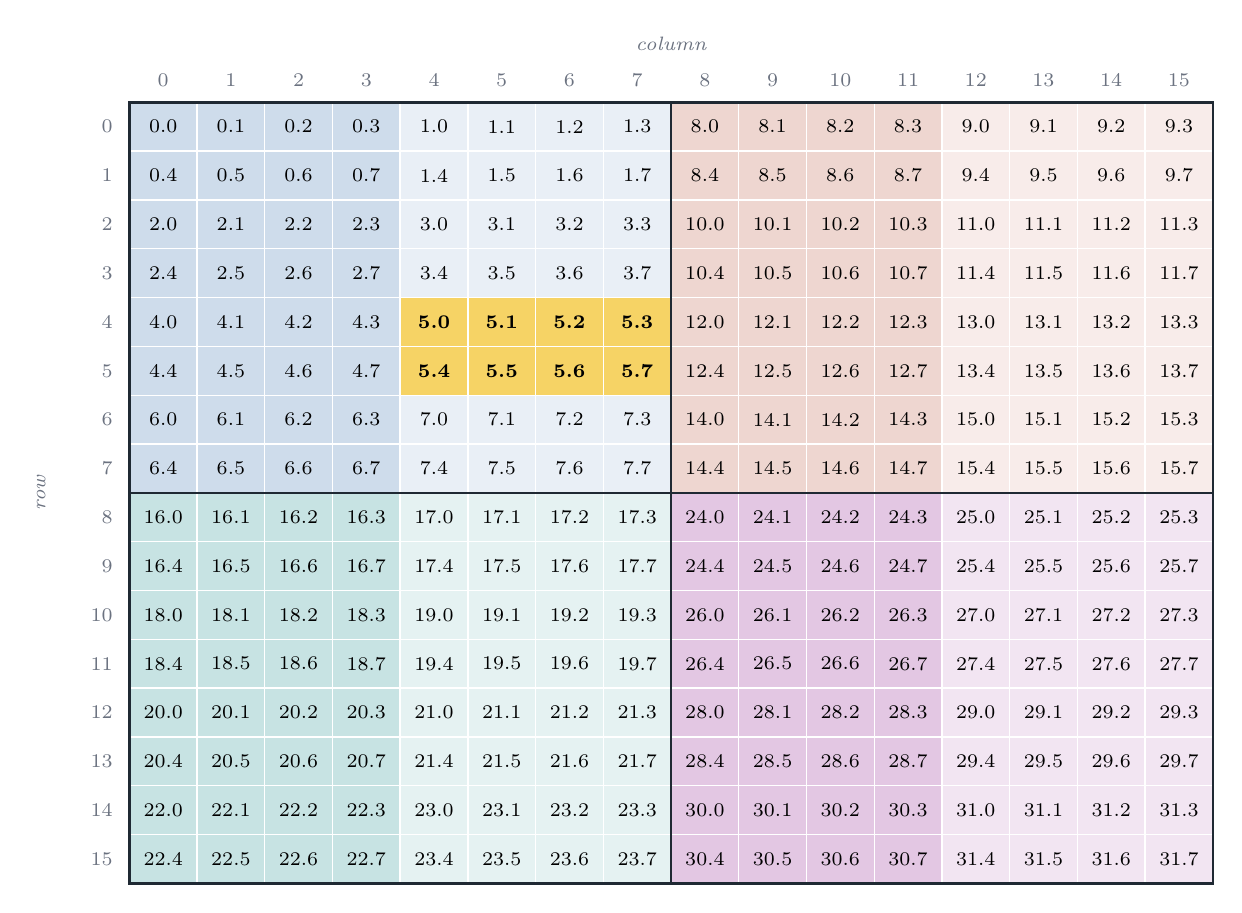
\begin{tikzpicture}[x=8.6mm, y=-6.2mm, font=\scriptsize]
  \node[text=apple] at (0.5,-0.45) {0};
  \node[text=apple] at (1.5,-0.45) {1};
  \node[text=apple] at (2.5,-0.45) {2};
  \node[text=apple] at (3.5,-0.45) {3};
  \node[text=apple] at (4.5,-0.45) {4};
  \node[text=apple] at (5.5,-0.45) {5};
  \node[text=apple] at (6.5,-0.45) {6};
  \node[text=apple] at (7.5,-0.45) {7};
  \node[text=apple] at (8.5,-0.45) {8};
  \node[text=apple] at (9.5,-0.45) {9};
  \node[text=apple] at (10.5,-0.45) {10};
  \node[text=apple] at (11.5,-0.45) {11};
  \node[text=apple] at (12.5,-0.45) {12};
  \node[text=apple] at (13.5,-0.45) {13};
  \node[text=apple] at (14.5,-0.45) {14};
  \node[text=apple] at (15.5,-0.45) {15};
  \node[text=apple, anchor=east] at (-0.1,0.5) {0};
  \node[text=apple, anchor=east] at (-0.1,1.5) {1};
  \node[text=apple, anchor=east] at (-0.1,2.5) {2};
  \node[text=apple, anchor=east] at (-0.1,3.5) {3};
  \node[text=apple, anchor=east] at (-0.1,4.5) {4};
  \node[text=apple, anchor=east] at (-0.1,5.5) {5};
  \node[text=apple, anchor=east] at (-0.1,6.5) {6};
  \node[text=apple, anchor=east] at (-0.1,7.5) {7};
  \node[text=apple, anchor=east] at (-0.1,8.5) {8};
  \node[text=apple, anchor=east] at (-0.1,9.5) {9};
  \node[text=apple, anchor=east] at (-0.1,10.5) {10};
  \node[text=apple, anchor=east] at (-0.1,11.5) {11};
  \node[text=apple, anchor=east] at (-0.1,12.5) {12};
  \node[text=apple, anchor=east] at (-0.1,13.5) {13};
  \node[text=apple, anchor=east] at (-0.1,14.5) {14};
  \node[text=apple, anchor=east] at (-0.1,15.5) {15};
  \fill[ours!22] (0,0) rectangle +(1,1); \node at (0.5,0.5) {0.0};
  \fill[ours!22] (1,0) rectangle +(1,1); \node at (1.5,0.5) {0.1};
  \fill[ours!22] (2,0) rectangle +(1,1); \node at (2.5,0.5) {0.2};
  \fill[ours!22] (3,0) rectangle +(1,1); \node at (3.5,0.5) {0.3};
  \fill[ours!10] (4,0) rectangle +(1,1); \node at (4.5,0.5) {1.0};
  \fill[ours!10] (5,0) rectangle +(1,1); \node at (5.5,0.5) {1.1};
  \fill[ours!10] (6,0) rectangle +(1,1); \node at (6.5,0.5) {1.2};
  \fill[ours!10] (7,0) rectangle +(1,1); \node at (7.5,0.5) {1.3};
  \fill[native!22] (8,0) rectangle +(1,1); \node at (8.5,0.5) {8.0};
  \fill[native!22] (9,0) rectangle +(1,1); \node at (9.5,0.5) {8.1};
  \fill[native!22] (10,0) rectangle +(1,1); \node at (10.5,0.5) {8.2};
  \fill[native!22] (11,0) rectangle +(1,1); \node at (11.5,0.5) {8.3};
  \fill[native!10] (12,0) rectangle +(1,1); \node at (12.5,0.5) {9.0};
  \fill[native!10] (13,0) rectangle +(1,1); \node at (13.5,0.5) {9.1};
  \fill[native!10] (14,0) rectangle +(1,1); \node at (14.5,0.5) {9.2};
  \fill[native!10] (15,0) rectangle +(1,1); \node at (15.5,0.5) {9.3};
  \fill[ours!22] (0,1) rectangle +(1,1); \node at (0.5,1.5) {0.4};
  \fill[ours!22] (1,1) rectangle +(1,1); \node at (1.5,1.5) {0.5};
  \fill[ours!22] (2,1) rectangle +(1,1); \node at (2.5,1.5) {0.6};
  \fill[ours!22] (3,1) rectangle +(1,1); \node at (3.5,1.5) {0.7};
  \fill[ours!10] (4,1) rectangle +(1,1); \node at (4.5,1.5) {1.4};
  \fill[ours!10] (5,1) rectangle +(1,1); \node at (5.5,1.5) {1.5};
  \fill[ours!10] (6,1) rectangle +(1,1); \node at (6.5,1.5) {1.6};
  \fill[ours!10] (7,1) rectangle +(1,1); \node at (7.5,1.5) {1.7};
  \fill[native!22] (8,1) rectangle +(1,1); \node at (8.5,1.5) {8.4};
  \fill[native!22] (9,1) rectangle +(1,1); \node at (9.5,1.5) {8.5};
  \fill[native!22] (10,1) rectangle +(1,1); \node at (10.5,1.5) {8.6};
  \fill[native!22] (11,1) rectangle +(1,1); \node at (11.5,1.5) {8.7};
  \fill[native!10] (12,1) rectangle +(1,1); \node at (12.5,1.5) {9.4};
  \fill[native!10] (13,1) rectangle +(1,1); \node at (13.5,1.5) {9.5};
  \fill[native!10] (14,1) rectangle +(1,1); \node at (14.5,1.5) {9.6};
  \fill[native!10] (15,1) rectangle +(1,1); \node at (15.5,1.5) {9.7};
  \fill[ours!22] (0,2) rectangle +(1,1); \node at (0.5,2.5) {2.0};
  \fill[ours!22] (1,2) rectangle +(1,1); \node at (1.5,2.5) {2.1};
  \fill[ours!22] (2,2) rectangle +(1,1); \node at (2.5,2.5) {2.2};
  \fill[ours!22] (3,2) rectangle +(1,1); \node at (3.5,2.5) {2.3};
  \fill[ours!10] (4,2) rectangle +(1,1); \node at (4.5,2.5) {3.0};
  \fill[ours!10] (5,2) rectangle +(1,1); \node at (5.5,2.5) {3.1};
  \fill[ours!10] (6,2) rectangle +(1,1); \node at (6.5,2.5) {3.2};
  \fill[ours!10] (7,2) rectangle +(1,1); \node at (7.5,2.5) {3.3};
  \fill[native!22] (8,2) rectangle +(1,1); \node at (8.5,2.5) {10.0};
  \fill[native!22] (9,2) rectangle +(1,1); \node at (9.5,2.5) {10.1};
  \fill[native!22] (10,2) rectangle +(1,1); \node at (10.5,2.5) {10.2};
  \fill[native!22] (11,2) rectangle +(1,1); \node at (11.5,2.5) {10.3};
  \fill[native!10] (12,2) rectangle +(1,1); \node at (12.5,2.5) {11.0};
  \fill[native!10] (13,2) rectangle +(1,1); \node at (13.5,2.5) {11.1};
  \fill[native!10] (14,2) rectangle +(1,1); \node at (14.5,2.5) {11.2};
  \fill[native!10] (15,2) rectangle +(1,1); \node at (15.5,2.5) {11.3};
  \fill[ours!22] (0,3) rectangle +(1,1); \node at (0.5,3.5) {2.4};
  \fill[ours!22] (1,3) rectangle +(1,1); \node at (1.5,3.5) {2.5};
  \fill[ours!22] (2,3) rectangle +(1,1); \node at (2.5,3.5) {2.6};
  \fill[ours!22] (3,3) rectangle +(1,1); \node at (3.5,3.5) {2.7};
  \fill[ours!10] (4,3) rectangle +(1,1); \node at (4.5,3.5) {3.4};
  \fill[ours!10] (5,3) rectangle +(1,1); \node at (5.5,3.5) {3.5};
  \fill[ours!10] (6,3) rectangle +(1,1); \node at (6.5,3.5) {3.6};
  \fill[ours!10] (7,3) rectangle +(1,1); \node at (7.5,3.5) {3.7};
  \fill[native!22] (8,3) rectangle +(1,1); \node at (8.5,3.5) {10.4};
  \fill[native!22] (9,3) rectangle +(1,1); \node at (9.5,3.5) {10.5};
  \fill[native!22] (10,3) rectangle +(1,1); \node at (10.5,3.5) {10.6};
  \fill[native!22] (11,3) rectangle +(1,1); \node at (11.5,3.5) {10.7};
  \fill[native!10] (12,3) rectangle +(1,1); \node at (12.5,3.5) {11.4};
  \fill[native!10] (13,3) rectangle +(1,1); \node at (13.5,3.5) {11.5};
  \fill[native!10] (14,3) rectangle +(1,1); \node at (14.5,3.5) {11.6};
  \fill[native!10] (15,3) rectangle +(1,1); \node at (15.5,3.5) {11.7};
  \fill[ours!22] (0,4) rectangle +(1,1); \node at (0.5,4.5) {4.0};
  \fill[ours!22] (1,4) rectangle +(1,1); \node at (1.5,4.5) {4.1};
  \fill[ours!22] (2,4) rectangle +(1,1); \node at (2.5,4.5) {4.2};
  \fill[ours!22] (3,4) rectangle +(1,1); \node at (3.5,4.5) {4.3};
  \fill[hilite] (4,4) rectangle +(1,1); \node at (4.5,4.5) {\textbf{5.0}};
  \fill[hilite] (5,4) rectangle +(1,1); \node at (5.5,4.5) {\textbf{5.1}};
  \fill[hilite] (6,4) rectangle +(1,1); \node at (6.5,4.5) {\textbf{5.2}};
  \fill[hilite] (7,4) rectangle +(1,1); \node at (7.5,4.5) {\textbf{5.3}};
  \fill[native!22] (8,4) rectangle +(1,1); \node at (8.5,4.5) {12.0};
  \fill[native!22] (9,4) rectangle +(1,1); \node at (9.5,4.5) {12.1};
  \fill[native!22] (10,4) rectangle +(1,1); \node at (10.5,4.5) {12.2};
  \fill[native!22] (11,4) rectangle +(1,1); \node at (11.5,4.5) {12.3};
  \fill[native!10] (12,4) rectangle +(1,1); \node at (12.5,4.5) {13.0};
  \fill[native!10] (13,4) rectangle +(1,1); \node at (13.5,4.5) {13.1};
  \fill[native!10] (14,4) rectangle +(1,1); \node at (14.5,4.5) {13.2};
  \fill[native!10] (15,4) rectangle +(1,1); \node at (15.5,4.5) {13.3};
  \fill[ours!22] (0,5) rectangle +(1,1); \node at (0.5,5.5) {4.4};
  \fill[ours!22] (1,5) rectangle +(1,1); \node at (1.5,5.5) {4.5};
  \fill[ours!22] (2,5) rectangle +(1,1); \node at (2.5,5.5) {4.6};
  \fill[ours!22] (3,5) rectangle +(1,1); \node at (3.5,5.5) {4.7};
  \fill[hilite] (4,5) rectangle +(1,1); \node at (4.5,5.5) {\textbf{5.4}};
  \fill[hilite] (5,5) rectangle +(1,1); \node at (5.5,5.5) {\textbf{5.5}};
  \fill[hilite] (6,5) rectangle +(1,1); \node at (6.5,5.5) {\textbf{5.6}};
  \fill[hilite] (7,5) rectangle +(1,1); \node at (7.5,5.5) {\textbf{5.7}};
  \fill[native!22] (8,5) rectangle +(1,1); \node at (8.5,5.5) {12.4};
  \fill[native!22] (9,5) rectangle +(1,1); \node at (9.5,5.5) {12.5};
  \fill[native!22] (10,5) rectangle +(1,1); \node at (10.5,5.5) {12.6};
  \fill[native!22] (11,5) rectangle +(1,1); \node at (11.5,5.5) {12.7};
  \fill[native!10] (12,5) rectangle +(1,1); \node at (12.5,5.5) {13.4};
  \fill[native!10] (13,5) rectangle +(1,1); \node at (13.5,5.5) {13.5};
  \fill[native!10] (14,5) rectangle +(1,1); \node at (14.5,5.5) {13.6};
  \fill[native!10] (15,5) rectangle +(1,1); \node at (15.5,5.5) {13.7};
  \fill[ours!22] (0,6) rectangle +(1,1); \node at (0.5,6.5) {6.0};
  \fill[ours!22] (1,6) rectangle +(1,1); \node at (1.5,6.5) {6.1};
  \fill[ours!22] (2,6) rectangle +(1,1); \node at (2.5,6.5) {6.2};
  \fill[ours!22] (3,6) rectangle +(1,1); \node at (3.5,6.5) {6.3};
  \fill[ours!10] (4,6) rectangle +(1,1); \node at (4.5,6.5) {7.0};
  \fill[ours!10] (5,6) rectangle +(1,1); \node at (5.5,6.5) {7.1};
  \fill[ours!10] (6,6) rectangle +(1,1); \node at (6.5,6.5) {7.2};
  \fill[ours!10] (7,6) rectangle +(1,1); \node at (7.5,6.5) {7.3};
  \fill[native!22] (8,6) rectangle +(1,1); \node at (8.5,6.5) {14.0};
  \fill[native!22] (9,6) rectangle +(1,1); \node at (9.5,6.5) {14.1};
  \fill[native!22] (10,6) rectangle +(1,1); \node at (10.5,6.5) {14.2};
  \fill[native!22] (11,6) rectangle +(1,1); \node at (11.5,6.5) {14.3};
  \fill[native!10] (12,6) rectangle +(1,1); \node at (12.5,6.5) {15.0};
  \fill[native!10] (13,6) rectangle +(1,1); \node at (13.5,6.5) {15.1};
  \fill[native!10] (14,6) rectangle +(1,1); \node at (14.5,6.5) {15.2};
  \fill[native!10] (15,6) rectangle +(1,1); \node at (15.5,6.5) {15.3};
  \fill[ours!22] (0,7) rectangle +(1,1); \node at (0.5,7.5) {6.4};
  \fill[ours!22] (1,7) rectangle +(1,1); \node at (1.5,7.5) {6.5};
  \fill[ours!22] (2,7) rectangle +(1,1); \node at (2.5,7.5) {6.6};
  \fill[ours!22] (3,7) rectangle +(1,1); \node at (3.5,7.5) {6.7};
  \fill[ours!10] (4,7) rectangle +(1,1); \node at (4.5,7.5) {7.4};
  \fill[ours!10] (5,7) rectangle +(1,1); \node at (5.5,7.5) {7.5};
  \fill[ours!10] (6,7) rectangle +(1,1); \node at (6.5,7.5) {7.6};
  \fill[ours!10] (7,7) rectangle +(1,1); \node at (7.5,7.5) {7.7};
  \fill[native!22] (8,7) rectangle +(1,1); \node at (8.5,7.5) {14.4};
  \fill[native!22] (9,7) rectangle +(1,1); \node at (9.5,7.5) {14.5};
  \fill[native!22] (10,7) rectangle +(1,1); \node at (10.5,7.5) {14.6};
  \fill[native!22] (11,7) rectangle +(1,1); \node at (11.5,7.5) {14.7};
  \fill[native!10] (12,7) rectangle +(1,1); \node at (12.5,7.5) {15.4};
  \fill[native!10] (13,7) rectangle +(1,1); \node at (13.5,7.5) {15.5};
  \fill[native!10] (14,7) rectangle +(1,1); \node at (14.5,7.5) {15.6};
  \fill[native!10] (15,7) rectangle +(1,1); \node at (15.5,7.5) {15.7};
  \fill[teal!22] (0,8) rectangle +(1,1); \node at (0.5,8.5) {16.0};
  \fill[teal!22] (1,8) rectangle +(1,1); \node at (1.5,8.5) {16.1};
  \fill[teal!22] (2,8) rectangle +(1,1); \node at (2.5,8.5) {16.2};
  \fill[teal!22] (3,8) rectangle +(1,1); \node at (3.5,8.5) {16.3};
  \fill[teal!10] (4,8) rectangle +(1,1); \node at (4.5,8.5) {17.0};
  \fill[teal!10] (5,8) rectangle +(1,1); \node at (5.5,8.5) {17.1};
  \fill[teal!10] (6,8) rectangle +(1,1); \node at (6.5,8.5) {17.2};
  \fill[teal!10] (7,8) rectangle +(1,1); \node at (7.5,8.5) {17.3};
  \fill[violet!22] (8,8) rectangle +(1,1); \node at (8.5,8.5) {24.0};
  \fill[violet!22] (9,8) rectangle +(1,1); \node at (9.5,8.5) {24.1};
  \fill[violet!22] (10,8) rectangle +(1,1); \node at (10.5,8.5) {24.2};
  \fill[violet!22] (11,8) rectangle +(1,1); \node at (11.5,8.5) {24.3};
  \fill[violet!10] (12,8) rectangle +(1,1); \node at (12.5,8.5) {25.0};
  \fill[violet!10] (13,8) rectangle +(1,1); \node at (13.5,8.5) {25.1};
  \fill[violet!10] (14,8) rectangle +(1,1); \node at (14.5,8.5) {25.2};
  \fill[violet!10] (15,8) rectangle +(1,1); \node at (15.5,8.5) {25.3};
  \fill[teal!22] (0,9) rectangle +(1,1); \node at (0.5,9.5) {16.4};
  \fill[teal!22] (1,9) rectangle +(1,1); \node at (1.5,9.5) {16.5};
  \fill[teal!22] (2,9) rectangle +(1,1); \node at (2.5,9.5) {16.6};
  \fill[teal!22] (3,9) rectangle +(1,1); \node at (3.5,9.5) {16.7};
  \fill[teal!10] (4,9) rectangle +(1,1); \node at (4.5,9.5) {17.4};
  \fill[teal!10] (5,9) rectangle +(1,1); \node at (5.5,9.5) {17.5};
  \fill[teal!10] (6,9) rectangle +(1,1); \node at (6.5,9.5) {17.6};
  \fill[teal!10] (7,9) rectangle +(1,1); \node at (7.5,9.5) {17.7};
  \fill[violet!22] (8,9) rectangle +(1,1); \node at (8.5,9.5) {24.4};
  \fill[violet!22] (9,9) rectangle +(1,1); \node at (9.5,9.5) {24.5};
  \fill[violet!22] (10,9) rectangle +(1,1); \node at (10.5,9.5) {24.6};
  \fill[violet!22] (11,9) rectangle +(1,1); \node at (11.5,9.5) {24.7};
  \fill[violet!10] (12,9) rectangle +(1,1); \node at (12.5,9.5) {25.4};
  \fill[violet!10] (13,9) rectangle +(1,1); \node at (13.5,9.5) {25.5};
  \fill[violet!10] (14,9) rectangle +(1,1); \node at (14.5,9.5) {25.6};
  \fill[violet!10] (15,9) rectangle +(1,1); \node at (15.5,9.5) {25.7};
  \fill[teal!22] (0,10) rectangle +(1,1); \node at (0.5,10.5) {18.0};
  \fill[teal!22] (1,10) rectangle +(1,1); \node at (1.5,10.5) {18.1};
  \fill[teal!22] (2,10) rectangle +(1,1); \node at (2.5,10.5) {18.2};
  \fill[teal!22] (3,10) rectangle +(1,1); \node at (3.5,10.5) {18.3};
  \fill[teal!10] (4,10) rectangle +(1,1); \node at (4.5,10.5) {19.0};
  \fill[teal!10] (5,10) rectangle +(1,1); \node at (5.5,10.5) {19.1};
  \fill[teal!10] (6,10) rectangle +(1,1); \node at (6.5,10.5) {19.2};
  \fill[teal!10] (7,10) rectangle +(1,1); \node at (7.5,10.5) {19.3};
  \fill[violet!22] (8,10) rectangle +(1,1); \node at (8.5,10.5) {26.0};
  \fill[violet!22] (9,10) rectangle +(1,1); \node at (9.5,10.5) {26.1};
  \fill[violet!22] (10,10) rectangle +(1,1); \node at (10.5,10.5) {26.2};
  \fill[violet!22] (11,10) rectangle +(1,1); \node at (11.5,10.5) {26.3};
  \fill[violet!10] (12,10) rectangle +(1,1); \node at (12.5,10.5) {27.0};
  \fill[violet!10] (13,10) rectangle +(1,1); \node at (13.5,10.5) {27.1};
  \fill[violet!10] (14,10) rectangle +(1,1); \node at (14.5,10.5) {27.2};
  \fill[violet!10] (15,10) rectangle +(1,1); \node at (15.5,10.5) {27.3};
  \fill[teal!22] (0,11) rectangle +(1,1); \node at (0.5,11.5) {18.4};
  \fill[teal!22] (1,11) rectangle +(1,1); \node at (1.5,11.5) {18.5};
  \fill[teal!22] (2,11) rectangle +(1,1); \node at (2.5,11.5) {18.6};
  \fill[teal!22] (3,11) rectangle +(1,1); \node at (3.5,11.5) {18.7};
  \fill[teal!10] (4,11) rectangle +(1,1); \node at (4.5,11.5) {19.4};
  \fill[teal!10] (5,11) rectangle +(1,1); \node at (5.5,11.5) {19.5};
  \fill[teal!10] (6,11) rectangle +(1,1); \node at (6.5,11.5) {19.6};
  \fill[teal!10] (7,11) rectangle +(1,1); \node at (7.5,11.5) {19.7};
  \fill[violet!22] (8,11) rectangle +(1,1); \node at (8.5,11.5) {26.4};
  \fill[violet!22] (9,11) rectangle +(1,1); \node at (9.5,11.5) {26.5};
  \fill[violet!22] (10,11) rectangle +(1,1); \node at (10.5,11.5) {26.6};
  \fill[violet!22] (11,11) rectangle +(1,1); \node at (11.5,11.5) {26.7};
  \fill[violet!10] (12,11) rectangle +(1,1); \node at (12.5,11.5) {27.4};
  \fill[violet!10] (13,11) rectangle +(1,1); \node at (13.5,11.5) {27.5};
  \fill[violet!10] (14,11) rectangle +(1,1); \node at (14.5,11.5) {27.6};
  \fill[violet!10] (15,11) rectangle +(1,1); \node at (15.5,11.5) {27.7};
  \fill[teal!22] (0,12) rectangle +(1,1); \node at (0.5,12.5) {20.0};
  \fill[teal!22] (1,12) rectangle +(1,1); \node at (1.5,12.5) {20.1};
  \fill[teal!22] (2,12) rectangle +(1,1); \node at (2.5,12.5) {20.2};
  \fill[teal!22] (3,12) rectangle +(1,1); \node at (3.5,12.5) {20.3};
  \fill[teal!10] (4,12) rectangle +(1,1); \node at (4.5,12.5) {21.0};
  \fill[teal!10] (5,12) rectangle +(1,1); \node at (5.5,12.5) {21.1};
  \fill[teal!10] (6,12) rectangle +(1,1); \node at (6.5,12.5) {21.2};
  \fill[teal!10] (7,12) rectangle +(1,1); \node at (7.5,12.5) {21.3};
  \fill[violet!22] (8,12) rectangle +(1,1); \node at (8.5,12.5) {28.0};
  \fill[violet!22] (9,12) rectangle +(1,1); \node at (9.5,12.5) {28.1};
  \fill[violet!22] (10,12) rectangle +(1,1); \node at (10.5,12.5) {28.2};
  \fill[violet!22] (11,12) rectangle +(1,1); \node at (11.5,12.5) {28.3};
  \fill[violet!10] (12,12) rectangle +(1,1); \node at (12.5,12.5) {29.0};
  \fill[violet!10] (13,12) rectangle +(1,1); \node at (13.5,12.5) {29.1};
  \fill[violet!10] (14,12) rectangle +(1,1); \node at (14.5,12.5) {29.2};
  \fill[violet!10] (15,12) rectangle +(1,1); \node at (15.5,12.5) {29.3};
  \fill[teal!22] (0,13) rectangle +(1,1); \node at (0.5,13.5) {20.4};
  \fill[teal!22] (1,13) rectangle +(1,1); \node at (1.5,13.5) {20.5};
  \fill[teal!22] (2,13) rectangle +(1,1); \node at (2.5,13.5) {20.6};
  \fill[teal!22] (3,13) rectangle +(1,1); \node at (3.5,13.5) {20.7};
  \fill[teal!10] (4,13) rectangle +(1,1); \node at (4.5,13.5) {21.4};
  \fill[teal!10] (5,13) rectangle +(1,1); \node at (5.5,13.5) {21.5};
  \fill[teal!10] (6,13) rectangle +(1,1); \node at (6.5,13.5) {21.6};
  \fill[teal!10] (7,13) rectangle +(1,1); \node at (7.5,13.5) {21.7};
  \fill[violet!22] (8,13) rectangle +(1,1); \node at (8.5,13.5) {28.4};
  \fill[violet!22] (9,13) rectangle +(1,1); \node at (9.5,13.5) {28.5};
  \fill[violet!22] (10,13) rectangle +(1,1); \node at (10.5,13.5) {28.6};
  \fill[violet!22] (11,13) rectangle +(1,1); \node at (11.5,13.5) {28.7};
  \fill[violet!10] (12,13) rectangle +(1,1); \node at (12.5,13.5) {29.4};
  \fill[violet!10] (13,13) rectangle +(1,1); \node at (13.5,13.5) {29.5};
  \fill[violet!10] (14,13) rectangle +(1,1); \node at (14.5,13.5) {29.6};
  \fill[violet!10] (15,13) rectangle +(1,1); \node at (15.5,13.5) {29.7};
  \fill[teal!22] (0,14) rectangle +(1,1); \node at (0.5,14.5) {22.0};
  \fill[teal!22] (1,14) rectangle +(1,1); \node at (1.5,14.5) {22.1};
  \fill[teal!22] (2,14) rectangle +(1,1); \node at (2.5,14.5) {22.2};
  \fill[teal!22] (3,14) rectangle +(1,1); \node at (3.5,14.5) {22.3};
  \fill[teal!10] (4,14) rectangle +(1,1); \node at (4.5,14.5) {23.0};
  \fill[teal!10] (5,14) rectangle +(1,1); \node at (5.5,14.5) {23.1};
  \fill[teal!10] (6,14) rectangle +(1,1); \node at (6.5,14.5) {23.2};
  \fill[teal!10] (7,14) rectangle +(1,1); \node at (7.5,14.5) {23.3};
  \fill[violet!22] (8,14) rectangle +(1,1); \node at (8.5,14.5) {30.0};
  \fill[violet!22] (9,14) rectangle +(1,1); \node at (9.5,14.5) {30.1};
  \fill[violet!22] (10,14) rectangle +(1,1); \node at (10.5,14.5) {30.2};
  \fill[violet!22] (11,14) rectangle +(1,1); \node at (11.5,14.5) {30.3};
  \fill[violet!10] (12,14) rectangle +(1,1); \node at (12.5,14.5) {31.0};
  \fill[violet!10] (13,14) rectangle +(1,1); \node at (13.5,14.5) {31.1};
  \fill[violet!10] (14,14) rectangle +(1,1); \node at (14.5,14.5) {31.2};
  \fill[violet!10] (15,14) rectangle +(1,1); \node at (15.5,14.5) {31.3};
  \fill[teal!22] (0,15) rectangle +(1,1); \node at (0.5,15.5) {22.4};
  \fill[teal!22] (1,15) rectangle +(1,1); \node at (1.5,15.5) {22.5};
  \fill[teal!22] (2,15) rectangle +(1,1); \node at (2.5,15.5) {22.6};
  \fill[teal!22] (3,15) rectangle +(1,1); \node at (3.5,15.5) {22.7};
  \fill[teal!10] (4,15) rectangle +(1,1); \node at (4.5,15.5) {23.4};
  \fill[teal!10] (5,15) rectangle +(1,1); \node at (5.5,15.5) {23.5};
  \fill[teal!10] (6,15) rectangle +(1,1); \node at (6.5,15.5) {23.6};
  \fill[teal!10] (7,15) rectangle +(1,1); \node at (7.5,15.5) {23.7};
  \fill[violet!22] (8,15) rectangle +(1,1); \node at (8.5,15.5) {30.4};
  \fill[violet!22] (9,15) rectangle +(1,1); \node at (9.5,15.5) {30.5};
  \fill[violet!22] (10,15) rectangle +(1,1); \node at (10.5,15.5) {30.6};
  \fill[violet!22] (11,15) rectangle +(1,1); \node at (11.5,15.5) {30.7};
  \fill[violet!10] (12,15) rectangle +(1,1); \node at (12.5,15.5) {31.4};
  \fill[violet!10] (13,15) rectangle +(1,1); \node at (13.5,15.5) {31.5};
  \fill[violet!10] (14,15) rectangle +(1,1); \node at (14.5,15.5) {31.6};
  \fill[violet!10] (15,15) rectangle +(1,1); \node at (15.5,15.5) {31.7};
  \foreach \i in {0,...,16} {\draw[white, line width=0.5pt] (\i,0) -- (\i,16); \draw[white, line width=0.5pt] (0,\i) -- (16,\i);}
  \draw[ink, line width=0.9pt] (0,0) rectangle (16,16) (8,0) -- (8,16) (0,8) -- (16,8);
  \node[text=apple, font=\scriptsize\itshape] at (8,-1.2) {column};
  \node[text=apple, font=\scriptsize\itshape, rotate=90] at (-1.3,8) {row};
\end{tikzpicture}
\caption{Lane and element slot of each element of a 16 × 16 A or D tile. Each cell is \emph{lane.slot}: the lane that holds the
element and which of its eight element slots it occupies (a half A fragment packs the eight slots into four registers,
an fp32 D into eight). The coordinates are canonical: the instruction's own, before any packing convention
(\cref{sec:coordinate-systems}). The four quadrants are the four groups of eight
lanes (blue, red, teal, violet: lanes 0--7, 8--15, 16--23 and 24--31); alternate lanes are shaded darker and
lighter to mark each lane's 2 × 4 block. Lane 5, the lane followed in \cref{sec:one-program-ir}, is
highlighted; this compiler's B-row packing stores those elements at application rows 2 and 10. The map was measured with one-hot probes over 6,651 dispatches (MM~\mm{3}); the figure is generated
from the formulas in \cref{sec:fragment-layouts}, which are checked against one another exactly.}
\label{fig:fragment-map}
\end{figure}


Lanes 0–7 hold rows 0–7 and columns 0–7, lanes 8–15 hold columns 8–15 of the same rows, and lanes 16–23 and 24–31 do the
same for rows 8–15. Within a quadrant each lane holds a 2 × 4 block of two adjacent rows and four adjacent columns,
slots 0–3 in the upper row and slots 4–7 in the lower. Because a lane's four slots in a row are consecutive columns, one
8-byte access per row loads them. Rows r and r + 8 sit in the two halves of the same lane group, which matches how the
tensor loads move an 8-row by 16-column sub-tile (\cref{sec:tensor-memory-path}).

The same map, by lane quadrant (MM~\mm{0.5}), is in \cref{tab:lane-quadrants}.

\begin{xltabular}{\linewidth}{@{}lllX@{}}
\caption{A/D fragment map by lane quadrant, with the rows and columns each eight-lane group holds.}\label{tab:lane-quadrants}\\
\toprule
Lanes & Rows & Columns & Within the eight-lane group, local lane q \\
\midrule
\endfirsthead
\tablecontinued{4}
\toprule
Lanes & Rows & Columns & Within the eight-lane group, local lane q \\
\midrule
\endhead
0–7 & 0–7 & 0–7 & rows \code{2*(q>>1)} and \code{+1}, columns \code{4*(q\&1)} to \code{+3} \\*
8–15 & 0–7 & 8–15 & same, column base +8 \\*
16–23 & 8–15 & 0–7 & same, row base +8 \\*
24–31 & 8–15 & 8–15 & same, both bases +8 \\*
\bottomrule
\end{xltabular}

A packer needs the inverse maps. Both are bijections onto the 256 (lane, slot) positions (re-verified, MM~\mm{3}):

\begin{lstlisting}
pos(r, c)   = (16*(r>>3) + 8*(c>>3) + 2*((r>>1)&3) + ((c>>2)&1),   4*(r&1) + (c&3))      A and D
pos_b(k, c) = (16*((k>>2)&1) + 8*(c>>3) + 2*(k&3) + ((c>>2)&1),     4*(k>>3) + (c&3))      B
\end{lstlisting}

Each returns (lane, slot).

\textbf{Worked example: four sample lanes} (derived from the formulas above). \Cref{tab:fragment-examples} gives the fragments of four
lanes.

\begin{longtable}{@{}rllll@{}}
\caption{A/D and B fragment contents of four sample lanes, derived from the layout formulas.}\label{tab:fragment-examples}\\
\toprule
Lane & A/D: slots 0–3 & A/D: slots 4–7 & B: slots 0–3 & B: slots 4–7 \\
\midrule
\endfirsthead
\tablecontinued{5}
\toprule
Lane & A/D: slots 0–3 & A/D: slots 4–7 & B: slots 0–3 & B: slots 4–7 \\
\midrule
\endhead
0 & D(0, 0..3) & D(1, 0..3) & B(0, 0..3) & B(8, 0..3) \\
9 & D(0, 12..15) & D(1, 12..15) & B(0, 12..15) & B(8, 12..15) \\
17 & D(8, 4..7) & D(9, 4..7) & B(4, 4..7) & B(12, 4..7) \\
22 & D(14, 0..3) & D(15, 0..3) & B(7, 0..3) & B(15, 0..3) \\
\bottomrule
\end{longtable}

Lane 22 step by step: \code{l>>4 = 1}, \code{(l>>1)\&3 = 11\&3 = 3}, \code{(l>>3)\&1 = 0}, \code{l\&1 = 0}. For A/D, \code{row = 8 + 6 + (j>>2)}
and \code{col = 0 + 0 + (j\&3)}, so slot 6 is D(15, 2). Inverse: \code{pos(15, 2) = (16*1 + 8*0 + 2*(7\&3) + ((2>>2)\&1), 4*(15\&1) + 2) = (22, 6)}. For B, \code{k = 4 + 3 + 8*(j>>2)}, so slot 6 is B(15, 2), and \code{pos\_b(15, 2) = (16*1 + 0 + 2*3 + 0, 4*1 + 2) = (22, 6)}. With transA = 1, lane 22 slot j holds A(row \code{2*(j\&3)}, k \code{7 + 8*(j>>2)}): slot 6 is
A(4, 15).

One fragment map serves all opcodes: \code{pos\_b(k, c) = pos(rotl1(k), c)} at 256 of 256 positions (measured,
re-verified, MM~\mm{3}). The B map is the A/D map with rows relabeled by a one-bit rotation. Check on lane 22: \code{rotl1(7) = 14} and \code{pos(14, 2) = (22, 2) = pos\_b(7, 2)}. Whether a destination "reads as pos or as pos\_b" depends only on the
row labeling used by the kernel that produced it (derived in \cref{sec:coordinate-systems}).

\emph{Withdrawn: two destination layouts.} The record once stated that the destination of the 16-bit MMA, \op{5106}, and its no-C sibling used a different layout from the fp32 × fp32 MMA, \op{5098},
because measured destinations of different kernels disagreed (recon section 100). A check for a fixed relabeling
between the two maps found that they differ exactly by \code{rotl1} on the row index at all 256 positions, the same
rotation Apple's cooperative-tensor coordinates carry. The difference came from the producing kernel's row labeling,
and the opcode claim was withdrawn (MM~\mm{3}, MM~\mm{19}). The same check later scoped the feed-mode
relabelings (\cref{sec:chaining-feed-modes}).

For other operand types (measured, MM~\mm{3}, MM~\mm{19}):

\begin{itemize}
\item fp32 and int8 operands use the same A, B and D maps as half.
\item \op{10384} is among 23 forms whose destination is \code{pos\_b} inside every 16 × 16
  tile with row-major tile blocks, 1,024 of 1,024 lane and slot (MM~\mm{3}). This describes Apple-compiled multi-tile
  destinations, consistent with the one-map rule above.
\item In the fp32 × fp32 MMA the fp32 A operand and the fp32 D/C share one layout (\code{A\_row == D\_row}, \code{A\_k == D\_col}, 256 of 256), so a D
  can feed the next A with no store and no permutation (MM~\mm{19}).
\item Apple's cooperative-tensor coordinates for a 16 × 16 single-simdgroup destination equal the B map with index 0 as
  column and index 1 as row; relative to the D map, rows are rotated by \code{y = ((r\&7)<<1) | (r>>3)} (Apple's compiler,
  MM~\mm{3}).
\end{itemize}

\Cref{tab:fragment-registers} gives register widths and legal bases (measured, MM~\mm{0.7}, MM~\mm{0.1}).

\begin{xltabular}{\linewidth}{@{}>{\hsize=1.39\hsize}X>{\hsize=0.63\hsize}XlX@{}}
\caption{Registers per lane, alignment and highest legal base register for scalars, fragments and accumulators.}\label{tab:fragment-registers}\\
\toprule
Value & Registers per lane & Alignment & Highest base \\
\midrule
\endfirsthead
\tablecontinued{4}
\toprule
Value & Registers per lane & Alignment & Highest base \\
\midrule
\endhead
scalar & 1 & 1 & R125 \\*
int8 or uint8 fragment & 2 & 2 & R124 \\*
half or bfloat fragment & 4 & 4 & R120 \\*
fp32 A or B fragment & 8 & 8 & R112 \\*
fp32 or int32 accumulator & 8 & 8 & R112 (15 groups: R0, R8, \dots{}, R112) \\*
\bottomrule
\end{xltabular}

R120–R127 cannot hold an 8-register group, because any instruction naming R126 or above is squashed whole
(\cref{sec:namespace}). MM~\mm{0.7} describes the int8 pair as "four byte elements per lane packed across the pair"; how the eight byte
elements of a lane are ordered within the pair is not stated in the sections this chapter draws on (open).

There is no tile-layout unit: a tensor load is a per-lane gather at an
ALU-computed address, and that arithmetic produces the layout (measured, MM~\mm{7}, MM~\mm{19}). Apple's library computes, once
per kernel, the index register \code{R32 = m(l)*128 + col(l)} with \code{m(l) = 4*(l>>4) + ((l>>1)\&3)} and
\code{col(l) = 8*((l>>3)\&1) + 4*(l\&1)}: element (m, col) of a row-major tile at leading dimension 128. Its loads read
\code{[R32*2 + disp]} with displacements \{0, 2048, 32, 4096, 6144\} (2048 steps eight rows, 32 steps sixteen columns). Each
access moves an 8-row by 16-column sub-tile, which is why rows r and r+8 sit in the two slot halves (Apple's compiler
emits, MM~\mm{7}). \emph{Correction:} "the hardware performs the matrix-to-fragment transposition" is refuted (MM~\mm{7}, MM~\mm{19}).

\textbf{Evidence.} MM~\mm{0.5}, MM~\mm{0.7}, MM~\mm{3}, MM~\mm{7}, MM~\mm{19}.

\section{Coordinate systems and packing}\label{sec:coordinate-systems}

Tensor code involves three kinds of coordinate, which have to be kept apart.

\begin{enumerate}
\item \emph{Canonical instruction coordinates}: the map from (lane, slot) to a matrix position that the MMA itself
  uses, \code{pos} for A and D and \code{pos\_b} for B (\cref{sec:fragment-layouts}). The MMA computes D = A B + C in
  these coordinates.
\item \emph{A kernel's packing convention}: which memory element its loads place in each (lane, slot), and where its stores
  write each slot. This is software: a tensor load is a per-lane gather at an address the kernel computes.
\item \emph{Application coordinates}: element (i, j) of the row-major matrix in memory.
\end{enumerate}

A kernel is correct when its packing convention, carried through the canonical arithmetic, produces the right product in
application coordinates. Two conventions are in use.

\begin{itemize}
\item \emph{Canonical packing.} Apple-compiled \code{simdgroup\_matrix} code packs A and D canonically (application row
  equals canonical row) and B canonically; the chaining relabelings were measured on such kernels (MM~\mm{3},
  MM~\mm{13}).
\item \emph{B-row packing.} This compiler packs every tile the same way, A, B and the C/D tile it loads and stores: lane l, slot j holds
  application row \code{m(l) + 8*(j>>2)} and column \code{col(l) + (j\&3)}, with \code{m(l) = 4*(l>>4) + ((l>>1)\&3)} and
  \code{col(l) = (l\&8) + 4*(l\&1)} (\code{agxforge/g17/indexgen.py}; \code{agxforge/g17/tlower.py}: "A rows m and m+8 of the tile, B rows k
  and k+8", stores "rows m and m+8"). This is the B map applied to every tile. Apple's tensor-ops library computes the same
  per-lane index for its tensor loads, and Apple-compiled multi-tile destinations read as \code{pos\_b}
  (\cref{sec:fragment-layouts}; MM~\mm{3}, MM~\mm{7}).
\end{itemize}

For B the two conventions agree. For A and D they differ by a one-bit rotation of the row index: because
\code{pos\_b(r, c) = pos(rotl1(r), c)}, this compiler puts application row r of A in canonical row \code{rotl1(r)}. The
rotation does not change the result. Rows of A are the free M index, so canonical row \code{rotl1(r)} of D holds application row r of
the product, and the store, which uses the same convention, writes canonical row \code{rotl1(r)} back to application row
r. Neither the columns nor the K index are permuted, so the reduction over K runs in canonical order and the result is
the one the arithmetic rule of \cref{sec:arithmetic-semantics-supported} predicts in application coordinates.

\textbf{Lane 5 of the running example.} In canonical coordinates its first MMA's D holds elements (4, 4)–(4, 7) in
slots 0–3 and (5, 4)–(5, 7) in slots 4–7 (\cref{fig:fragment-map}). This compiler computes \code{m(5) = 2} and
\code{col(5) = 4}, so its store writes slots 0–3 to application row 2 and slots 4–7 to row 10, columns 4–7. The two
descriptions name the same registers: \code{rotl1(2) = 4} and \code{rotl1(10) = 5}.

\textbf{D fed as B.} A feed hands D's registers unchanged to the next
MMA as its B operand. The MMA reads lane l, slot j as canonical B row \code{k = 4*(l>>4) + ((l>>1)\&3) + 8*(j>>2)}, and
that register holds canonical D row \code{rotl1(k)}.

\begin{itemize}
\item Under B-row packing (this compiler), canonical D row \code{rotl1(k)} is application row k of the product, so the
  consumer reads \code{B\_eff[k][c] = D[k][c]}: the logical operand, with no instruction in between.
\item Under canonical packing, canonical D row \code{rotl1(k)} is application row \code{rotl1(k)}, so the consumer reads
  \code{B\_eff[k][c] = D[rotl1(k)][c]}: the row-rotated operand that \cref{sec:chaining-feed-modes} measures, which the other
  operand's K index must then be permuted to undo.
\end{itemize}

\Cref{tab:coordinate-example} follows three slots through both conventions. For lane 0, slot 4, canonical D row 1 is
read as B row 8; this compiler's producer placed application row \code{m(0) + 8 = 8} of D in that slot, so the consumer
receives D row 8 as B row 8. With canonical packing the same register carries D row 1, and \code{rotl1(8) = 1}. A D fed
as A needs no relabeling in either convention, because the consumer's A is packed the way the producer packed D.

\begin{longtable}{@{}lllll@{}}
\caption{Three slots in canonical coordinates and in the two packing conventions, for a D tile fed as the next B.}\label{tab:coordinate-example}\\
\toprule
Lane, slot & Canonical D & Read as B & D row, B-row packing & D row, canonical packing \\
\midrule
\endfirsthead
\tablecontinued{5}
\toprule
Lane, slot & Canonical D & Read as B & D row, B-row packing & D row, canonical packing \\
\midrule
\endhead
0, 4 & (1, 0) & (8, 0) & 8 & 1 \\*
5, 0 & (4, 4) & (2, 4) & 2 & 4 \\*
5, 4 & (5, 4) & (10, 4) & 10 & 5 \\*
\bottomrule
\end{longtable}

So the relabeling a feed needs is set by the producer's packing alone. The two measurements agree with this derivation (\cref{sec:chaining-feed-modes}): in this compiler's kernels
the B, At and Bt feeds read the logical operand bit for bit and a reference that applied the relabelings failed, in the
one square 32 × 32 stage measured (MM~\mm{25.103}); in canonically packed kernels the feeds follow the fixed relabelings,
the identity for A (MM~\mm{13}).

\section{Arithmetic by input type}\label{sec:arithmetic-semantics-supported}

Each result below is labelled an \textbf{exact rule} (a closed form that reproduces every measured output) or a
\textbf{measured case} (single points or edge values); unresolved behaviour is marked open.

\textbf{Half inputs, fp32 accumulator: exact rule} (measured, MM~\mm{4}, MM~\mm{0.6}; fitted on half × half, 1,680 of 1,680
eps-triples and every stimulus). For one output element, with \code{k} the A-column index of \cref{sec:fragment-layouts}:

\begin{lstlisting}
p_i = RNE32(a[2i]*b[2i] + a[2i+1]*b[2i+1])      i = 0..7    adjacent pairs; products exact
q_j = RNE32(p_j + p_(j+4))                       j = 0..3    pairs eight apart
acc = C
acc = RNE32(acc + q_0); acc = RNE32(acc + q_1); acc = RNE32(acc + q_2); acc = RNE32(acc + q_3)
D   = acc
\end{lstlisting}

\Cref{fig:reduction-tree} shows the measured order.

% Figure 10.2: the measured reduction order of one output element of a 16x16x16 MMA
% (MM 4, MM 0.6). Every node rounds to nearest-even fp32.
\begin{figure}[htbp]
\centering
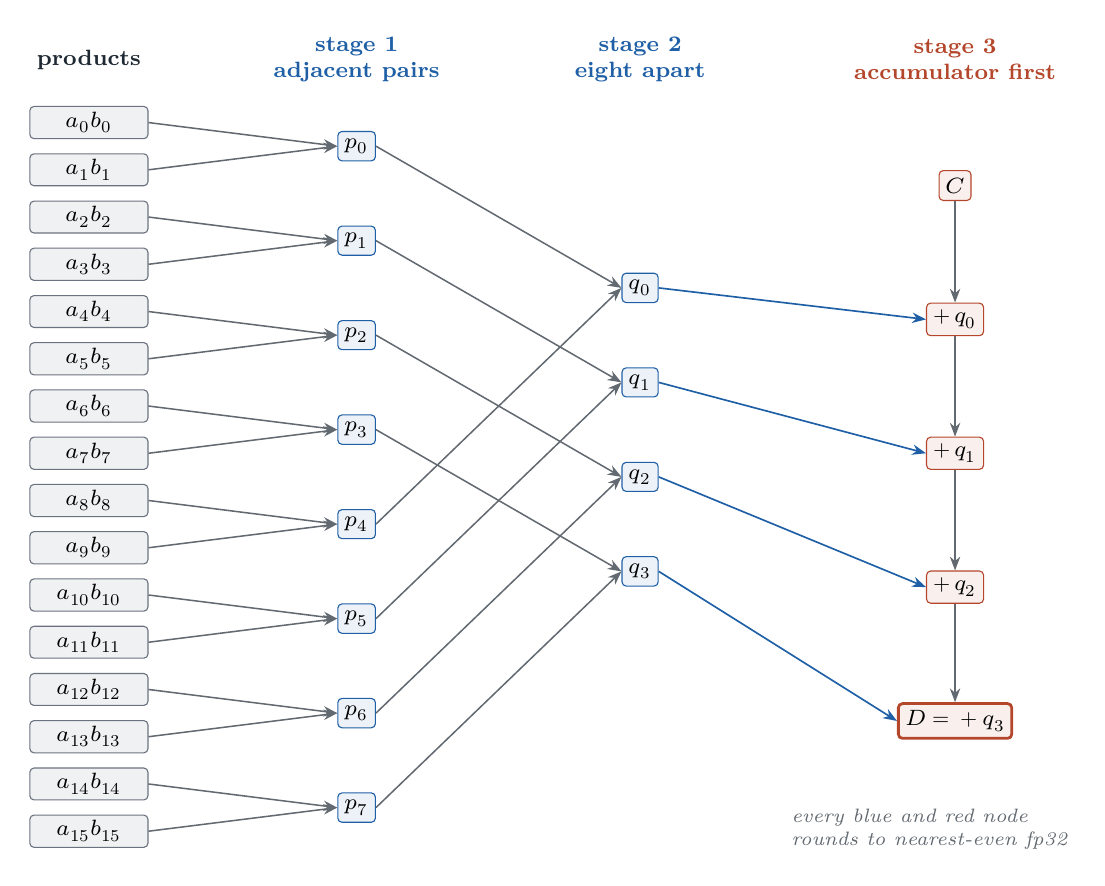
\begin{tikzpicture}[x=1mm, y=-1mm, font=\footnotesize,
    prod/.style={draw=apple, fill=apple!10, rounded corners=1.5pt, inner sep=2pt, minimum width=15mm},
    add/.style={draw=ours, fill=ours!8, rounded corners=1.5pt, inner sep=2.5pt, align=center},
    acc/.style={draw=native, fill=native!8, rounded corners=1.5pt, inner sep=2.5pt, align=center},
    e/.style={->, line width=0.55pt, color=ink!70}]
  % stage headings
  \node[font=\footnotesize\bfseries, text=ink] at (8,-8) {products};
  \node[font=\footnotesize\bfseries, text=ours, align=center] at (42,-8) {stage 1\\adjacent pairs};
  \node[font=\footnotesize\bfseries, text=ours, align=center] at (78,-8) {stage 2\\eight apart};
  \node[font=\footnotesize\bfseries, text=native, align=center] at (118,-8) {stage 3\\accumulator first};
  % sixteen exact products, two per stage-1 node
  \foreach \i in {0,...,15} {
    \pgfmathtruncatemacro\k{\i}
    \node[prod] (x\i) at (8, 6*\i) {$a_{\k} b_{\k}$};
  }
  % stage 1: p_i = RNE(a_{2i}b_{2i} + a_{2i+1}b_{2i+1})
  \foreach \i in {0,...,7} {
    \pgfmathtruncatemacro\a{2*\i}\pgfmathtruncatemacro\b{2*\i+1}
    \node[add] (p\i) at (42, 12*\i+3) {$p_{\i}$};
    \draw[e] (x\a.east) -- (p\i.west);
    \draw[e] (x\b.east) -- (p\i.west);
  }
  % stage 2: q_i = RNE(p_i + p_{i+4})
  \foreach \i in {0,...,3} {
    \pgfmathtruncatemacro\j{\i+4}
    \node[add] (q\i) at (78, 12*\i+21) {$q_{\i}$};
    \draw[e] (p\i.east) -- (q\i.west);
    \draw[e] (p\j.east) -- (q\i.west);
  }
  % stage 3: C enters first, then q0..q3 in a chain
  \node[acc] (C) at (118, 8) {$C$};
  \node[acc] (s0) at (118, 25) {$+\,q_0$};
  \node[acc] (s1) at (118, 42) {$+\,q_1$};
  \node[acc] (s2) at (118, 59) {$+\,q_2$};
  \node[acc, line width=1pt] (D) at (118, 76) {$D = {}+q_3$};
  \draw[e] (C) -- (s0);
  \draw[e] (s0) -- (s1); \draw[e] (s1) -- (s2); \draw[e] (s2) -- (D);
  \foreach \i/\s in {0/s0, 1/s1, 2/s2, 3/D} \draw[e, ours] (q\i.east) -- (\s.west);
  % rounding note
  \node[font=\scriptsize\itshape, text=ink!70, align=left, anchor=north west] at (96, 86)
    {every blue and red node\\rounds to nearest-even fp32};
\end{tikzpicture}
\caption{The measured reduction of one output element. One 16 × 16 × 16 MMA computes each output element from
sixteen exact products. Stage 1 adds adjacent products, $p_i = \mathrm{RNE}_{32}(a_{2i}b_{2i} + a_{2i+1}b_{2i+1})$;
stage 2 adds partial sums eight products apart, $q_i = \mathrm{RNE}_{32}(p_i + p_{i+4})$; stage 3 starts from the
accumulator $C$ and adds $q_0, \dots, q_3$ in order, rounding at every step. The from-zero form, \op{5107}, has no
$C$ and starts the chain from $q_0$. The diagram shows data dependence, not physical adders (MM~\mm{4},
MM~\mm{0.6}).}
\label{fig:reduction-tree}
\end{figure}


The tree is neither balanced nor sequential. The first stage adds adjacent products, which is why \code{(-0) * 1}, with every
other product zero, gives \code{+0} (the signed-zero case below). The second stage pairs partial sums eight apart. The
accumulator then enters before the four partial sums, within one issue. The from-zero form, \op{5107}, follows the same tree without C and starts the chain from q0 ("starts from the first reduced
group", MM~\mm{0.3}).

\textbf{How the tree was identified.} The candidates were a sequential chain, a balanced tree over the natural K order, a
balanced tree over K interleaved by eight and an exactly rounded sum, and, for the accumulator, adding C first or last.
They differ only in the order of additions and where rounding happens, so the stimuli were placed on single output elements
with half inputs, whose products are always exact in fp32 (an 11-bit by 11-bit significand product fits in 24 bits, and
every such product lies between $2^{-48}$ and about $4.3 \times 10^{9}$, inside fp32's normal range). A single-element
stimulus then isolates the order of additions and the rounding. The main probe was the \textbf{eps-triple}: one product
equal to 1 at a K position i and products equal to a small eps at two other positions j and k, over every placement
(16 × 105 = 1,680 stimuli). Whether the two eps terms are added to each other before either meets the 1 changes the
rounded result, so each triple answers one question about the tree's shape (MM~\mm{4}; the triple design is from the
record's section 4, which MM~\mm{4} cites).

\begin{itemize}
\item Rival fits on the 1,680 triples: balanced tree on natural order 976, interleave-by-8 balanced tree 1,392, the rule
  above 1,680. The triples fixed the pair and interleave stages.
\item Round-to-nearest-even applies at every intermediate; round-toward-zero is rejected on every stimulus.
\item Over a whole tile: 5,120 of 5,120 exact, against sequential 2,493, balanced 2,764, exact sum rounded
  once 2,742. Re-confirmed later with no correction (MM~\mm{4}).
\item Stimuli built for the purpose placed C; the worked example below shows how one separates C-first from C-last.
\end{itemize}

\textbf{Worked example: why C enters first} (executed on hardware for the measured value; the arithmetic below is the rule
applied by hand). Let eps = $2^{-24}$, half an fp32 ulp at 1.0. Take C = 1.0 and choose products so that the first two
quad sums are q\_0 = q\_1 = 3 eps and q\_2 = q\_3 = 0 (for example products eps at K positions 0, 1 and 8 give
p\_0 = 2 eps, p\_4 = eps, so q\_0 = 3 eps exactly; positions 2, 3 and 10 do the same for q\_1; eps = $2^{-12}$ × $2^{-12}$, both
normal half values).

\begin{lstlisting}
C first (the measured rule):
  acc = RNE32(1 + 3 eps)       = 1 + 4 eps     1.5 ulp is a tie; RNE picks the even neighbour, 2 ulp
  acc = RNE32(1 + 4 eps + 3 eps) = 1 + 8 eps   3.5 ulp is a tie; RNE picks the even neighbour, 4 ulp
C last (any order that sums the q terms first):
  q_0 + q_1 = 6 eps exactly;  RNE32(1 + 6 eps) = 1 + 6 eps   3 ulp, representable
\end{lstlisting}

Adding C first exposes each small partial sum to a tie against 1.0; summing the q terms first keeps them exact and
rounds once. The hardware returns \code{1 + 8 eps} on the discriminating stimuli (measured, MM~\mm{4}), which rules out every
model that adds C at the end, including an exactly rounded sum.

\textbf{Checks against independent code.} The repository's
bit-exact model \code{tools/tensorops-model/tensorops\_model.py}, which was not used to fit the rule, reproduces Apple's 32×32×64 library kernel on 6,144 of 6,144
elements (exact-sum-rounded-once: 1,948) and a previously failed tile on 1,024 of 1,024; Apple's \code{matmul2d} is
bit-exact to it on all eight shapes of the speed comparison (measured, MM~\mm{4}, MM~\mm{25.98}). The converse failure was
also seen: this project's tensor runtime once used a reference MMA that added C after the products, and the released
\code{multigemm} class had been failing its own exact check on 417 of 1,024 elements for that reason (MM~\mm{25.89}).

\textbf{Accumulate-mode composition in Apple's library: exact rule} (measured, MM~\mm{4}, MM~\mm{0.6},
MM~\mm{15}). The library's own accumulate mode orders C the other way. With a nonzero C, \code{matmul2d}'s
multiply-accumulate mode runs the MMA chain from zero and then loads C and adds it with ordinary fp32 adds (product
first, C last), one extra rounding compared with putting C in the first MMA. The one-rounding difference between that
mode and a single MMA with C has the same cause as the worked example. This describes how the library composes calls;
inside one issue C still enters first, so a reference that models \code{matmul2d} needs both orders, and a compiler that
puts C in the first MMA will differ from the library's accumulate mode by that rounding.

\textbf{Longer K: exact rule} (measured, MM~\mm{4}). Issues compose through the rounded fp32 accumulator: two-issue chains
reproduce the rule applied twice on 17 of 17 stimuli, three-issue chains 17 of 17; an unrounded inter-issue
accumulator is rejected (8 of 17, 12 of 17). K order is ascending in memory whether the library unrolls or loops: for
K=64, chunk orders 3210, 0213 and 1032 are each rejected by at least one stimulus; a K=128 runtime loop gives
\code{1 + 6eps} on seven asymmetric probes where descending gives \code{1 + 8eps}.

\textbf{Other input types: measured cases.} The machine model states that bfloat and truncated-fp32
operands follow the same tree (MM~\mm{0.6}, MM~\mm{5}), but the discriminating fit above was made on half inputs only.
Their products are exact only while fp32 can hold them, and unlike half products they can leave fp32's range. The
record has single points at the extremes, not a rule: a bfloat product at $2^{-133}$ or $2^{-140}$ (fp32 subnormals) is
kept, a bfloat product of 3e38 × 3e38 gives Inf, a truncated-fp32 product $2^{100} \times 2^{-100}$ is exactly 1, and
truncated-fp32 subnormal operands keep their surviving bits (recon section 33; MM~\mm{5}).

\textbf{fp32 operands: exact rule} (measured, MM~\mm{5}). An fp32 A or B is masked, not rounded: the low 13 bits of the raw
pattern are cleared, keeping sign, 8 exponent bits and 10 fraction bits, for normals and subnormals alike (TF32-shaped
truncation toward zero). \code{1 + 2\textasciicircum{}-10 + 2\textasciicircum{}-11} becomes \code{1 + 2\textasciicircum{}-10}; \code{2 - 2\textasciicircum{}-23} becomes \code{2 - 2\textasciicircum{}-10}; the full exponent
range survives (\code{2\textasciicircum{}100 * 2\textasciicircum{}-100 = 1} exactly). The truncated operands then follow the same tree. The fp32-operand forms
cost no issue rate over the half forms (measured, MM~\mm{8}; \cref{ch:performance}).

\begin{itemize}
\item \emph{Correction:} "fp32 operand subnormals flush to zero" (recon section 5; MM~\mm{19}) is withdrawn: only the low 13 bits are
  cleared. The module docstring of \code{tools/tensorops-model/tensorops\_model.py} (line 12, "subnormals flushed") still
  carries the old reading; its \code{to\_f32\_operand} docstring and code (\code{\& 0xffffe000}) keep subnormals, matching MM~\mm{5}.
\end{itemize}

\textbf{Subnormals: measured cases} (measured, MM~\mm{5}). In the recorded cases nothing in the half or bfloat path or the accumulator flushes: half
\code{2\textasciicircum{}-24 * 1} gives \code{2\textasciicircum{}-24}; a bfloat product at \code{2\textasciicircum{}-140} is kept; an fp32 accumulator subnormal passes through. fp32
ALU operations flush subnormal inputs and results (MM~\mm{5}, MM~\mm{17} rule 22; \cref{ch:scalar-arithmetic}), so a subnormal
the MMA produces is flushed to zero by the next fp32 ALU instruction that reads it.

\textbf{Special values: measured cases} (measured, MM~\mm{5}).

\begin{itemize}
\item The 51 recorded edge cases (recon section 33; MM~\mm{5}) give, case by case: NaN × 1, NaN × 0, Inf × 0, Inf + (−Inf)
  inside the sum, and a NaN in C each yield the fp32 quiet NaN \code{0x7fc00000}; Inf × 1 yields Inf; a bfloat product past
  fp32's maximum (3e38 × 3e38) yields Inf; C = fp32 max plus 1 stays fp32 max.
\item half \code{65504 * 65504 = 4.29e9} exactly, and sixteen such products sum exactly.
\item A NaN in an A column poisons the result even where the matching B row is zero, so K padding must be zeros
  (MM~\mm{17} rule 14).
\item Whether Inf − Inf gives the canonical NaN at every position of the tree, and which NaN payloads survive, is not
  recorded beyond these cases (open).
\end{itemize}

\textbf{Signed zero: measured case} (measured, MM~\mm{5}). \code{(-0) * 1} with every other term zero gives \code{+0}, because the pair
stage adds a neighbouring \code{+0} first under RNE; a model with \code{(-0) + (-0) = -0} mispredicts.

\textbf{int8 inputs, int32 accumulator: exact rule} (measured, MM~\mm{5}, MM~\mm{11}). Products are exact, with signedness selected
independently for A and B. The default form accumulates modulo $2^{32}$ with no saturation, including inside one MMA:
\code{C + 2\textasciicircum{}31} gives \code{-2\textasciicircum{}31}, and \code{16*127*127 + INT\_MAX} wraps to −2147225585. 608 accumulators were exact modulo $2^{32}$ out
to a million iterations in all four sign combinations, 429 of them after leaving the int32 range. One K=16 tile cannot
overflow on its own (16 × 16,384 = 262,144).

\textbf{Saturating int8: exact rule} (measured, MM~\mm{11}, MM~\mm{25.42}, MM~\mm{25.89}).

\begin{itemize}
\item One MMA computes \code{D = clip(C + A.B, -2\textasciicircum{}31, 2\textasciicircum{}31 - 1)}: one signed clip of the exact sixteen-term sum, also for
  unsigned operands, which saturate at the signed limit. The rule scored 2,400 of 2,400 tiles in every sign
  combination; wrapping scored 1,746, 1,759, 1,742 and 2,129, staged saturation 1,975, 1,886, 1,897 and 2,400. The
  unsigned-by-unsigned column (the last) cannot discriminate, because every product is non-negative; the signed cases
  carry the result. Saturation is not sticky.
\item Under transpose, with D seeded to \code{INT32\_MAX - 32} and all-ones int8 operands (exact sum 2147483679), wrap
  predicts −2147483617 and saturation 2147483647. With A transposed, Apple's bytes (byte8 0x44) give −2147483617 on all
  1,024 outputs; with byte8 bit 4 set on all sixteen \op{10384} instances (0x54), 2147483647 on all 1,024; an in-range sum
  (64) is unchanged by the bit (MM~\mm{25.42}). The untransposed pair (0x40, 0x50) behaves the same.
\item A chain of saturating MMAs clips once per issue: on inputs near both rails, wrap, clip after every
  product, clip after every issue and clip once at the end differ pairwise on 21 to 56 of 1,024 elements, and the
  hardware matched clip-per-issue (MM~\mm{25.89}).
\item \emph{Correction:} MM~\mm{20} ("Correctness hazards left open") says saturation with transposes, chains and high registers
  "was not run"; its own inline note marks this stale. Transposes were run in MM~\mm{25.42} and chains in MM~\mm{25.89}: saturation
  applies per issue and is independent of the transpose bits.
\end{itemize}

\textbf{Destination conversions: exact rules} (measured, MM~\mm{5}, MM~\mm{6}, MM~\mm{0.6}, MM~\mm{17} rule 21). These are the conversion
instructions a kernel applies to the fp32 accumulator, not part of the MMA. Over 1,510,400 fp32 patterns:

\begin{itemize}
\item fp32 to half is IEEE round-to-nearest-even with zero mismatches, subnormal results included (\code{65520} goes to
  infinity, \code{2\textasciicircum{}-25} to zero).
\item fp32 to bfloat is RNE except that an fp32 subnormal input returns a zero carrying the input's sign (5,879 of
  5,912 subnormal patterns).
\item Every NaN input maps to one canonical NaN per type: half \code{0x7e00}, bfloat \code{0x7fc0}.
\item Denormal and fast-math settings change none of this.
\end{itemize}

\textbf{16-bit destinations across calls: measured case} (measured, MM~\mm{12}, MM~\mm{17} rule 18). A 16-bit destination rounds
after every accumulating library call: four contributions to a half destination give 2054 where one rounding gives
2052; the same contributions inside one call with K=64 give 2052, because internal K slices stay fp32. Use a float
destination across calls.

In every tested route, fp8, int4 and scaled inputs are reached through conversions in front of these forms; see \cref{sec:quantized-formats}.

To match the hardware bit for bit, a reference model has to add C first inside an issue (the rule fitted on half
inputs), truncate fp32 operands rather than round them, carry subnormals through the MMA (in the measured cases) and
wrap int32 accumulation by default; an ordinary dot product gets the bits wrong, as do the sequential and exactly
rounded rivals above.

\textbf{Evidence.} MM~\mm{0.6}, MM~\mm{4}, MM~\mm{5}, MM~\mm{6}, MM~\mm{11}, MM~\mm{12}, MM~\mm{15}, MM~\mm{17}, MM~\mm{19}, MM~\mm{25.42}, MM~\mm{25.89}, MM~\mm{25.98}.

\section{Ordering and the tensor enable}\label{sec:ordering-enable}

\subsection*{Ordering}

The scoreboard's semantics (slots, wait masks, slot choice and reuse, what an unwaited consumer reads) are
\cref{sec:scoreboard}'s, and the carriers of every field are \cref{sec:scoreboard-publish-wait}'s. What is specific to the tensor unit:

\begin{itemize}
\item A tensor MMA carries an 8-bit wait mask at flags bits 24–31: for a load filling slot \code{s}, the consuming MMA must
  set bit \code{24 + s} (measured, MM~\mm{6}, MM~\mm{0.8}). The bits are physically scattered (slot 7 is
  byte0{[}3{]}; \cref{sec:scoreboard-publish-wait}). In the running example (\cref{sec:one-program-ir}) all eight tile loads fill slot 0 and each MMA's
  flags word is 0x01000000, bit 24.
\item \emph{Earlier reading as a result ring.} The same bits were first read as an eight-slot
  "result ring" of in-flight results: in Apple's code each compiled MMA waited on exactly its own load group, so the bits
  looked one-hot and positional (MM~\mm{6}, MM~\mm{19}; the correction is told in \cref{sec:scoreboard-publish-wait,sec:scoreboard}).
  The wait-mask reading ties each bit to the slot a load fills, and predicting each consumer's bit from its load's slot
  was confirmed 20 of 20 (preregistered, MM~\mm{6}). In the removal control, clearing byte0{[}3{]} on an
  MMA whose operands come from slot 7 makes it read fragments before the loads land; it produces zeros
  deterministically (50 of 50 dispatches across five processes for tensor loads) (measured, MM~\mm{6}, MM~\mm{17} rule 4).
  An unmasked slot is not waited on, and nothing reports it. \textbf{Silent.} An emitter must set the wait bit of every
  slot that an operand's load fills; this can be checked from the decoded bytes alone.
\item The tensor load names the slot it fills in operand 1 bits 20–23, as slot + 1, a different carrier from the ordinary
  \op{12709} (measured, MM~\mm{6}, MM~\mm{25.4/R6} "R6 closed and B2 decoded"; \cref{sec:scoreboard-publish-wait}).
\item On the result side, an ALU instruction placed directly after an MMA, with no wait, read the MMA's result correctly;
  whether the hardware interlocks MMA-to-ALU or the consuming form waits implicitly is open (MM~\mm{6}, MM~\mm{25.90}). In
  this compiler's kernels an ALU read right after the last MMA needed no extra wait and was bit-exact (this compiler, measured,
  MM~\mm{25.105.1}). Assume the pattern holds for the measured kernels and no further; it is not a proven interlock.
\item Feeding D as the next MMA's C, A or B in the same simdgroup needs no wait in the measured forms, and no
  instruction when the consumer takes fp32; a 16-bit consumer needs eight narrowings (\cref{sec:chaining-feed-modes}; measured,
  MM~\mm{0.9}, MM~\mm{13}).
\item Tensor store (\opn{17257}, 876 instances) and masked tensor store (\opn{17258}, 118 instances) carry a
  zero wait byte in every compiled instance, yet immediate MMA-to-store paths are exact (measured and decoder, MM~\mm{6}; \cref{sec:scoreboard}).
\item \emph{Hazards caused by the host harness.} Two apparent MMA hazards (a stored result feeding a register-resident consumer;
  independent back-to-back MMAs) were the harness's \code{dim} parameter, which bounds how many output bytes are complete
  and host-visible on return; both kernels pass when it covers the output (\code{dim\textasciicircum{}2 * esz}) (MM~\mm{19}, MM~\mm{17} rule 5).
\item Slot assignment past eight load groups and slot reuse follow \cref{sec:scoreboard}; this compiler's K=256 half and int8
  lowerings (16 K slices, slots reused two to three times) match Apple and the reference in all three trials (measured,
  MM~\mm{6}, MM~\mm{20}).
\end{itemize}

\subsection*{Per-kernel metadata slot 44}

The enable's effect was measured by patching 14 pipelines (MM~\mm{6}, MM~\mm{0.1}). The metadata format is in
\cref{ch:kernel-metadata-image}.

\begin{itemize}
\item Slot 44 is present exactly when the code contains a tensor MMA: in all 50 such kernels and in no legacy-engine
  kernel. That correlation alone could be bookkeeping that follows from the code; the patches below show it is required.
\item If its low byte is zero, every tensor MMA produces zeros, the pipeline still builds and the dispatch completes
  without error. In the tested patches any nonzero low byte, with the other three bytes arbitrary, is bit-identical
  to the original, so the low byte acts as an on/off switch.
\item A disabled unit produces zeros quickly and neither faults nor stalls: a 1,400-MMA chain runs in 14.75~µs
  instead of 32.0 (8.4~ns per issue instead of 22), a saturated dispatch in 0.587~ms instead of 22.7 (a factor of 39).
  The MMAs still issue, at roughly ALU cost, while writing zeros. The timing fits a power or clock gate better than a
  validity check; the mechanism itself was not measured.
\item An image author must give every kernel that contains a tensor MMA the enable with a nonzero low byte. A zero low byte is not refused at pipeline build and shows up only as zero results.
  \textbf{Silent.}
\item With an explicit imageblock in the same kernel, per-kernel slot 19 sits at 55 and the tensor enable moves to slot 54;
  the slot-29 vector is {[}48, 49, 52{]} (Apple's compiler emits, MM~\mm{25.89}). "Slot 44" is the position in the
  tensor-only layout, not a fixed index in every kernel.
\end{itemize}

Metal caches pipelines by AIR function hash, so a pipeline built earlier in the same process is
reused and every byte patched into the archive afterwards silently does nothing. Build the archive in one process, and
patch and dispatch in another, with a positive control that shows a predictable bit moving the output (measured,
MM~\mm{17} rule 36, MM~\mm{25.42}).

\textbf{Evidence.} MM~\mm{0.1}, MM~\mm{0.8}, MM~\mm{6}, MM~\mm{13}, MM~\mm{17}, MM~\mm{20}, MM~\mm{25.4/R6} "R6 closed and B2 decoded", MM~\mm{25.42}, MM~\mm{25.89},
MM~\mm{25.90}, MM~\mm{25.105.1}.

\section{Tensor loads and stores}\label{sec:tensor-memory-path}

The tensor unit has no memory port of its own. Fragments are filled and drained by per-lane loads and stores at
addresses ordinary ALU code computes; partial tiles are handled by masks, not by the MMA (measured, MM~\mm{7}). The general
memory mechanisms (addressing, displacement folding, threadgroup memory) live in \cref{ch:memory}; bandwidth and latency
figures in \cref{ch:performance}.

\Cref{tab:tensor-load-store} lists the tensor load and store forms (measured, MM~\mm{0.8}, MM~\mm{7}).

\begin{xltabular}{\linewidth}{@{}XXX@{}}
\caption{Tensor load and store forms, with per-lane payload and mask kind.}\label{tab:tensor-load-store}\\
\toprule
Form & Per-lane payload & Mask \\
\midrule
\endfirsthead
\tablecontinued{3}
\toprule
Form & Per-lane payload & Mask \\
\midrule
\endhead
\op{12674} & two 32-bit words, four 16-bit elements; 12- or 16-byte encoding & immediate (15 or 0) \\*
\op{12675} & two words & 16-bit register \\*
\op{12656} & one word, four int8 elements, byte-addressed & immediate \\*
\op{12657} & one word & 16-bit register \\*
\op{12692} & fp32 elements (element width 4) & not stated in the sources \\*
\op{17257} & four 32-bit words & immediate \\*
\op{17258} & four words & 16-bit register: bit j enables word j (j = 0..3); bits above 3 ignored;
unwritten words keep their prior contents \\*
\bottomrule
\end{xltabular}

An int8 operand needs the byte-addressed one-word form, not the generic four-word load (measured, MM~\mm{7}).

The operand list of the tensor load and the tensor store is (decoder only, MM~\mm{7})
\code{dst, mode imm, flag imm, base (a relocation expression naming the buffer), imm, index:GPR32, last-use imm, byte-offset imm, element code, mask}.

\begin{itemize}
\item The element code is the access width in bytes: 1 for the int8 one-word load, 2 for half (all 7,853 half/bf16 tensor-load
  instances carry 2), 4 for float (the fp32 tensor load and plain float accesses), and 8 and 16 for wider accesses (16
  witnessed on \op{12709} and \op{17256}) (measured and decoder, MM~\mm{7}, MM~\mm{25.37}).
  \emph{Correction:} MM~\mm{25.5/R7}
  "R7 narrowed" is superseded by MM~\mm{25.37} on code 4 (\cref{app:a}).
\item In Apple's code the mask is only 15 or 0 and last-use only 0 or 16 (Apple's compiler emits, MM~\mm{7}). The last-use
  immediate follows the index register and takes the release modifier's values (\cref{sec:modifiers-keep-flag}); a reader should treat 16
  as releasing the index register.
\item Field positions from a single-bit census: the mode field's variable content is byte11{[}3{]}; the index register is a
  7-bit selector at byte3{[}1..7{]}; the byte offset is byte8{[}5..7{]} plus byte9{[}0..4{]} (decoder only, MM~\mm{7}).
\item The slot the load fills is operand 1 bits 20–23, as slot + 1 (\cref{sec:ordering-enable}). A load can also carry a wait mask, used so the
  first tile loads wait on the index register's own load (measured, MM~\mm{6}).
\end{itemize}

The row stride is not an instruction field. A non-default stride changes the mode immediate from 241 to
2289 (bit 11 of the mode word), switches to a per-lane computed index register and adds ALU code; the stride lives in
the register's precomputed value (decoder and Apple's compiler, MM~\mm{7}). Default strides must come from the operand's
element size: a lowering that used \code{K*2} for every type was twice too small for float and twice too large for int8,
and the 32×32×64 int8 case was wrong on 1,024 of 1,024 elements (measured, MM~\mm{17} rule 6). \textbf{Silent.}

Partial tiles are masked with \op{612}, whose 8-bit \code{lo} and width immediates
make masks tile-relative (measured, MM~\mm{7}, MM~\mm{19}; semantics in \cref{sec:masks-predicated-memory}). Multi-simdgroup sub-tile ownership is
expressed as per-simdgroup store masks (Apple's compiler emits, MM~\mm{7}).

A tensor load is a per-lane gather whose addressing is \cref{sec:fragment-layouts}'s; displacements are bytes
(\cref{sec:address-computation}; MM~\mm{25.141.18}). \code{air.simdgroup\_async\_copy\_2d} lowers to a synchronous load/store loop and its wait to
nothing; latency hiding is the scoreboard (Apple's compiler emits, MM~\mm{25.89}).

Through Metal, the one fault seen (\cref{sec:out-of-range-accesses-observed}) came from a \code{regprobe\_multi} tensor-kernel
probe whose configuration was not recorded (measured, MM~\mm{17} rule 34, as corrected there); size every buffer from the
kernel's own layout. A dead load's destination is still in flight, and reusing it lets the late load overwrite it
(measured, MM~\mm{25.114}).

\textbf{Evidence.} MM~\mm{0.8}, MM~\mm{6}, MM~\mm{7}, MM~\mm{17}, MM~\mm{19}, MM~\mm{25.37}, MM~\mm{25.89}, MM~\mm{25.114}, MM~\mm{25.141.18}.

\section{Chaining and the memory bridge}\label{sec:chaining-feed-modes}

A feed hands one MMA's destination D (8 fp32 registers per lane) to a later MMA in the same simdgroup without a
store. There are four modes: D as A, as B, as A with transA ("At") and as B with transB ("Bt"); D can
also be the next C (the ordinary K chain).

An fp32 D fed into an fp32 operand needs no instruction (measured, MM~\mm{13}); a 16-bit consumer needs
exactly eight conversions, \op{1016}, per D tile. The direct chain is bit-identical to the
memory bridge on 200 of 200 random matrices (204,800 elements).

The measured relabelings admit two readings: a property of the MMA's operand ports, which every compiler must apply,
or a consequence of how the producing kernel packed its tiles. \Cref{sec:coordinate-systems} derives the second, which
predicts different feeds for the two packings in use. One measurement per packing separates the two:

\begin{enumerate}
\def\labelenumi{\arabic{enumi}.}
\item In kernels that pack A and D canonically (Apple-compiled \code{simdgroup\_matrix} code), register-direct chaining is
  exact in all four modes with fixed relabelings: 1,596 of 1,596 random chained pairs over four modes, five operand
  forms and grids from 1×1 to 4×4, extended to 304 of 304 over eight grids and five transpose combinations (measured,
  MM~\mm{13}, MM~\mm{0.10}):

  \begin{lstlisting}
  fed as A            A_eff[r][k] = D[r][k]
  fed as B            B_eff[k][c] = D[rotl1(k)][c]
  fed as A, transA    A_eff[r][k] = D[rotl1(k)][rotr1(r)]
  fed as B, transB    B_eff[k][c] = D[rotl1(c)][k]
  \end{lstlisting}

  A logical \code{A2 . D1} through the B feed then needs A2 loaded with its k index permuted by \code{rotl1} (wrong in 20 of 20
  trials without it), and matches the unpermuted product to rounding, not bit for bit, because the permutation changes
  the association order. In the transposed feeds the accumulator C must carry the same relabeling (MM~\mm{17} rules 9–11).
\item In kernels that use B-row packing for every tile (this compiler's \code{tlower} emission), every feed reads the
  logical operand bit for bit (measured, MM~\mm{25.103}): B computes \code{A2 . D}, At computes \code{D\textasciicircum{}T . B2}, Bt computes
  \code{A2 . D\textasciicircum{}T}. The test was preregistered with the relabeled product as the prediction and the logical
  product as the control expected to fail. The relabeled reference failed in every arm, with maximum errors of 290 (B), 305 (At) and 477 (Bt), and the logical product was bit-exact. The two references differ on
  1,024, 1,024 and 896 of 1,024 elements (Bt's remaining 128 are columns where \code{rotl1(c) = c}), so the test could
  separate them. Decoded, At differs from A only in operand 5 (the type field with the transpose bit) and, off the
  diagonal, the fed register. The domain is one square stage (M = N = 32, K = 64), one simdgroup, no accumulate, with
  the fed operand in fp32 or narrowed to half; mode A was measured separately in this compiler's chains (MM~\mm{25.89}).
\end{enumerate}

Both measurements place the relabelings in the producer's packing. A compiler applies them only when the producer packed D
canonically; under B-row packing of every tile, D included, it applies none (MM~\mm{17} rule 9 as scoped by MM~\mm{25.103}),
and B, At and Bt feeds outside the measured stage remain unmeasured. \emph{Correction:} the relabeling table read as an instruction property (MM~\mm{0.10},
MM~\mm{13} before their scope notes) is scoped by MM~\mm{25.103}.

Other feed cases have been measured:

\begin{itemize}
\item \emph{Accumulator (C) feed} (this compiler, measured, MM~\mm{25.125.2}): the register C feed is bit-identical to the memory
  bridge (M32 and M16, 3 of 3 each; swapped-tile and claims-no-C controls fail on 1,024 of 1,024). At M32 it removes
  eight fp32 C loads and the producer's eight stores but splits the consumer into two accumulator groups; the
  instruction count is unchanged (192).
\item \emph{int8 chains}: in hand-authored AIR (Apple's labeling), int8 accumulators, including register-resident requantized
  chains, chain through all four modes with the half chain's rotations, 272 of 272 runs (measured, MM~\mm{3}, MM~\mm{11}).
\item \emph{Transposed consumers across a quantize boundary} inside a hidden-chunk loop: nn reads \code{Pt.W}, tn \code{P.W}, nt
  \code{Pt.Wt}, tt \code{P.Wt}, 12 runs exact (measured, MM~\mm{25.45}).
\item \emph{S and P kept in registers} for prefill attention (a register-fed A from a named accumulator): exact (measured,
  MM~\mm{25.163}; the time saved is in \cref{sec:bounds-real-workloads}).
\item \emph{Staging D through the imageblock} is bit-exact but frees no registers and is slower: register feed 13.4 / 20.3~µs,
  memory bridge 14.6 / 23.3~µs, imageblock 14.4 / 27.3~µs at M16 / M64; staging adds 254 instructions at M64
  (measured, MM~\mm{25.106}).
\end{itemize}

Two earlier readings were host errors (MM~\mm{19}). That \code{matmul2d} allows one \code{run()} per kernel and that a
chain must cross a kernel boundary was a misreading of slice offsets, which are (column, row); read correctly, both
calls are bit-exact in one kernel. And certain operand ranges once excluded from register-direct chaining were errors
of the host model, which rounded each product where the hardware forms products exactly; no operand-range condition
remains.

This compiler emits a feed only for a receipted key
(producer and consumer form with every modifier, role A/B/C, transpose, tile grid, locality), all one simdgroup and
one threadgroup (this compiler, MM~\mm{25.125.3}, MM~\mm{0.10}); any absent key stays on the memory bridge. A decoded chain containing any stack store is not
register-resident (MM~\mm{17} rule 12).

Apple's library has a chaining hazard (measured, MM~\mm{13}, MM~\mm{17} rule 13). Its cooperative input tensor exposes only the
first \code{min(\#D1 tiles, \#D2 tiles)} blocks of the producer in row-major block order; a narrower consumer silently reads
zeros or wrong elements for the rest. The rule predicts all 27 configurations measured per side (M and both widths in 16, 32
and 64, one simdgroup), of which the nine narrower consumers per side fail; \code{is\_compatible\_as\_*\_input}, a run-time
member function of \code{matmul2d}, returns true in every one, so it cannot serve as a guard. Pad the consumer to the producer's tile count or use the memory bridge. \textbf{Silent.}

The memory bridge, a tensor store to row-major memory followed by a tensor load, worked in every measured case
(measured, MM~\mm{13}): two separately generated bodies joined at a buffer offset are bit-exact, including a
cross-lane stress and a K remainder. In one kernel and one simdgroup it needs no fence, because the second body's
loads follow the first body's stores in program order on the same scoreboard. It is the correctness baseline and the
default outside the receipted feed domain. Streaming the free tile axis runs grids up to 12×8 producing 12×12 (1,344
MMAs, 4,807 instructions) with zero stack stores; spill edges are not a closed-form function of shape (two
preregistered rules failed at 6 of 12 and 82 of 144).

\textbf{Evidence.} MM~\mm{0.10}, MM~\mm{3}, MM~\mm{11}, MM~\mm{13}, MM~\mm{17}, MM~\mm{25.45}, MM~\mm{25.103}, MM~\mm{25.106}, MM~\mm{25.125.2}, MM~\mm{25.125.3},
MM~\mm{25.163}.

\section{Data movement across simdgroups}\label{sec:across-simdgroups}

Registers did not cross a simdgroup in any measured case. A cross-simdgroup \code{simd\_shuffle} returns the caller's own simdgroup's value in
256 of 256 cases. Only the accumulator role can stay register-resident across simdgroups, and only inside one library
cooperative scope where both simdgroups take part in both calls; no register state crosses a simdgroup boundary there
either (measured, MM~\mm{14}).

A hand-off between simdgroups takes three steps (measured, MM~\mm{14}, MM~\mm{17} rule 7):

\begin{enumerate}
\def\labelenumi{\arabic{enumi}.}
\item a fragment-order store (16 bytes per lane for a converted A or B tile, 32 for an fp32 accumulator);
\item a workgroup barrier: with no barrier, or with \code{air.simdgroup.barrier} alone, the hand-off is wrong in 12 of 12
  trials; every workgroup barrier variant (execution-only, threadgroup memory, device memory, both) is correct in 12
  of 12. Without one the consumer reads exactly zero, the buffer's pre-write state. That an execution-only barrier
  sufficed is an observation about this chip, not a memory-model guarantee; \cref{sec:barriers-fences} says what each barrier
  orders. \textbf{Silent} when omitted;
\item a fragment-order load, which returns the producer's register bits in the same lane and slot: no relayout exists.
\end{enumerate}

The round costs roughly a quarter of a microsecond including both barriers (measured, MM~\mm{14}). Store + barrier + load
per round: 38.0~ns at one simdgroup and one threadgroup per core, 81.9~ns at 32 simdgroups, 100–131~ns at 64 per core
through threadgroup memory; through device memory 58–83~ns and 151–161~ns (1 percent above threadgroup memory at low
occupancy, 17 percent at high) (measured, MM~\mm{7}). Threadgroup and device memory are within 8 percent in the scheduling
study (MM~\mm{14}).

Three scheduling rules follow from the measurements (216 of 216 exact, MM~\mm{14}, MM~\mm{17} rule 32):

\begin{itemize}
\item never recompute a shared stage per simdgroup (1.16 to 6.66 times the shared time);
\item share at low occupancy (1.7 to 10 times faster than one simdgroup holding all tiles), and when one simdgroup would
  hold 16 fp8 output tiles and spill 134–138 stores;
\item otherwise keep the tiles in one simdgroup (sharing costs 3 to 22 percent).
\end{itemize}

Shared fused stages are exact through 16 simdgroups (measured, MM~\mm{0.14}, MM~\mm{20}); at 32 the recompute form
stays exact but both shared forms exceed the 32 KiB threadgroup-memory limit. Sharing between threadgroups needs a
dispatch boundary; a threadgroup that waits on another inside one dispatch depends on both being resident, which is
the restriction of \cref{sec:forward-progress-in-order}.

At \code{execution\_simdgroups<2>} and \code{<4>} the library partitions output tiles per simdgroup with no barrier and no
threadgroup memory (Apple's compiler emits, MM~\mm{25.93}; \cref{sec:it-reached}). This
compiler's \code{gemm\_generic} admits 2 and 4 simdgroups and up to 8 threadgroups, bit-exact on hardware (this compiler,
MM~\mm{0.13}, MM~\mm{25.89}).

\textbf{Evidence.} MM~\mm{0.14}, MM~\mm{7}, MM~\mm{14}, MM~\mm{17}, MM~\mm{20}, MM~\mm{25.89}, MM~\mm{25.93}.

\section{Quantized formats}\label{sec:quantized-formats}

Of the ten admitted forms, none takes an fp8 or sub-8-bit operand and none applies a block scale. In every route
tested (Apple's compiler, Apple's library, hand-written AIR), low-precision formats reach the unit by conversion into
an int8, half or bfloat fragment with ordinary instructions, and scales are applied in software. This describes the
recovered forms and the routes tried, not a complete inventory of the hardware.

int8 and uint8 are native (measured, MM~\mm{0.11}, MM~\mm{8}, MM~\mm{11}): \op{10384} and its
no-C form, at exactly twice the fp16 issue rate (\cref{sec:tensor-issue-rate}). Arithmetic in \cref{sec:arithmetic-semantics-supported}.

Requantization from int32 to int8 has no instruction; it is a scalar sequence (load, integer to float, multiply,
round, float to integer, clamp, store) (measured, MM~\mm{11}). Rounding is round-half-to-even (±0.5, 1.5, 2.5, 3.5 give
0, 2, 2, 4); the clamp saturates (32768 gives 127, not −128; −25600 gives 0, not 156). This compiler's requant
epilogue computes \code{b = acc + bias[col]} (int32, wrapping), \code{f = float32(b)} (RNE), \code{y = float32(f*scale)} (RNE),
\code{r = rint(y)} (half-even), \code{q = clamp(r + zp, lo, hi)}, lowered as \op{10282}, \op{11179}, \op{3290}, \op{3770}, a clamp to \code{[lo-zp, hi-zp]} with \op{9700} before narrowing, \op{9320}, and a second 32-bit add for the zero point
(this compiler, measured, MM~\mm{25.130.1}).

\begin{itemize}
\item The float-to-int conversion saturates at both widths, signed and unsigned, and sends NaN to 0; a prior
  \code{maxnum}/\code{minnum} clamp is harmful (it maps a NaN block to −127). Guard with \code{isnan(x)} or
  \code{(as\_type<uint>(x) \& 0x7fffffff) > 0x7f800000}; under default fast math \code{x != x} folds to false (measured, MM~\mm{6},
  MM~\mm{17} rule 17). \textbf{Silent.}
\end{itemize}

For fp8 (e4m3fn and e5m2), eight \op{17642} instructions, each
taking two fp8 values in a 16-bit register to two bf16 values in a 32-bit register (format immediate 97 for e4m3fn, 98
for e5m2), feed one ordinary bf16 use of the 16-bit MMA (measured, MM~\mm{11}). Decode is exact for all 254 finite e4m3fn codes and 248
finite e5m2 codes; arithmetic is bit-identical to the bf16 rule on 96 of 96 tiles across four format pairs;
transposes exact on 36 of 36. Cost: bf16's when the unpack is hoisted (4.96~ns per MMA per core, 14 accumulators); 5.3
ns at four unpacked fragments per MMA and 8.4~ns at eight. Keep unpacked fragments per MMA at four or fewer (MM~\mm{17} rule
28).

For packing, \op{13618} (AIR \code{air.convert}) rounds to nearest even with no
saturation (measured, MM~\mm{11}, MM~\mm{25.105}, MM~\mm{25.105.1}), verified over all $2^{32}$ fp32 patterns and all 65,536
bf16 and fp16 patterns. Largest finite values are 448 (e4m3fn) and 57,344 (e5m2). Signed zeros are kept. \Cref{tab:fp8-pack-limits} gives the
results at and beyond the range limits and for NaN.

\begin{xltabular}{\linewidth}{@{}>{\hsize=1.58\hsize}X>{\hsize=0.74\hsize}X>{\hsize=0.68\hsize}X@{}}
\caption{fp8 pack results for large magnitudes and NaN inputs, by target format.}\label{tab:fp8-pack-limits}\\
\toprule
Input & e4m3fn result & e5m2 result \\
\midrule
\endfirsthead
\tablecontinued{3}
\toprule
Input & e4m3fn result & e5m2 result \\
\midrule
\endhead
magnitude rounds to 448 or less (464 itself rounds to 448) & RNE code & – \\*
magnitude above 464, positive & 0x7f (NaN) & – \\*
magnitude above 464, negative & 0xff (NaN, sign kept) & – \\*
magnitude 61,440 or above, positive & – & 0x7c (+infinity) \\*
magnitude 61,440 or above, negative & – & 0xfc (−infinity) \\*
NaN input, either sign & 0x7f & 0x7e \\*
\bottomrule
\end{xltabular}

An fp8 overflow keeps its sign; only NaN inputs become the positive canonical NaN. Two e4m3fn overflow arms whose
reference sent every overflow to 0x7f failed in exactly the negative overflows (174 of 372, 297 of 575); with the
sign kept, both arms match word for word, and e5m2's 963 overflows were signed infinities (measured, MM~\mm{25.105}). The
quantize-out epilogue of this compiler and the pack measured in MM~\mm{11} are the same instruction, the fp8 pack, so the
rule covers both. \emph{Correction:} MM~\mm{0.11}'s quantizer table ("Above 464 → canonical NaN") is superseded for negative
overflows by MM~\mm{25.105} (corrected at MM~\mm{25.105.1}); MM~\mm{11}'s "Every NaN input maps to the positive canonical NaN" is about
NaN inputs only and stands.

Apple's fp8 store encoding (Apple's compiler emits, MM~\mm{25.105.1}): per eight floats, four packs of the 12-byte form of
fp8 pack, vector, from fp32/half/bf16 (\code{op13618/12}), each
writing one 16-bit half from two fp32 registers in place (\code{R4L <- R4, R5}, then \code{R4H <- R6, R7}, where R4–R7 are four
accumulator registers), then one \op{17202} per packed register (width 4, index \code{lane*5}).

int4 and uint4 likewise reach no admitted form directly (measured and Apple's compiler, MM~\mm{5}, MM~\mm{25.6},
MM~\mm{25.28}). Nibbles
are unpacked by ordinary ALU instructions, for example \op{435}, \op{437} and
\op{11183} with the integer-to-float conversions, into a supported fragment, then the 16-bit MMA,
\op{5106}, or the int8 MMA. int2 needs no new mechanism; its refusal is at the
\code{tensor\_inline} constructor, an API limit (MM~\mm{25.6}). \emph{Correction:} the two AND forms were once read as shifts.

No tested route reaches fp4 (e2m1) or fp6 (e2m3, e3m2) in hardware (bounded negative and Apple's compiler, MM~\mm{0.11}, MM~\mm{20},
MM~\mm{25.94}): no vendor route tested produced a hardware unpack, pack or MMA for them. After a software decode the ordinary fp16 or
bf16 use of the 16-bit MMA applies; the decode costs about 24 instructions per value in Apple's newer backend and about 4 in MLX's bit
trick. Packed fp4 and fp6 tokens crash \code{buildConvert}; \code{air.pack} and \code{air.unpack} crash \code{buildPack};
\code{air.quantize\_pack} crashes \code{NumericPackUnpackPass}. This compiler has not built the software operand unpack (MM~\mm{0.14}).

No tested route applies a block scale in hardware (measured, MM~\mm{11}, MM~\mm{17} rule 26). The scaled \code{matmul2d} form is MX-style: a \code{ue8m0}
scale per 32 elements along K, one plane per row of A and per column of the transposed B, no bias, no zero point. The
eleven-operand scaled intrinsic compiles but has no effect: across 36 configurations with scale exponents from $2^{-30}$
to $2^{+30}$, every output equals the unscaled result and the emitted 16-bit MMA bytes are identical; per-lane scale operands
are dropped silently. Never emit the scaled spelling expecting scaling. \textbf{Silent.} The scaled int8 form with fp32
accumulate aborts at \code{Failed to encode.} (Apple's compiler, MM~\mm{20}).

Scaling in software was measured for placement and cost (MM~\mm{11}, MM~\mm{25.105.2}):

\begin{itemize}
\item \emph{Cheapest placement:} per 32-element K block, two MMAs into a zeroed temporary (the first is \op{5107}), then one
  fp32 multiply-add of the block sum by the product of the two scales: 8 instructions per MMA, 1.03 to 1.08 times the
  unscaled MMA time on 2×2 to 4×2 grids; 477 byte-table plus 128 predecoded comparisons bit-identical.
\item \emph{Latency hiding:} the block's MMAs do not depend on the accumulator, so the multiply-add's round trip hides behind
  the next block's MMAs. Against a chained form it costs 8~ns per step (15 percent), where a multiply-add inside the
  dependent path costs about 27~ns per step at low occupancy; the forms converge at 12 or more simdgroups per core.
\item \emph{Operand-side scaling:} 5.7 to 10.1~ns against 5.0~ns per MMA, 74 percent of elements exact for one block;
  the integer exponent add is wrong for zeros and subnormals.
\item \emph{This compiler's MX step} (\code{mx32}) uses the post-MMA placement with \code{T = (T * SA) * SB} then \code{D += T} (two fp32
  multiplies and an fp32 add). The multiplies are exact while the result stays in fp32's normal range, because the
  factors are powers of two; a result below $2^{-126}$ is flushed by the ALU (\cref{sec:fp32-arithmetic}), and the add
  into D rounds as any fp32 add does. The step is bit-exact for e4m3 × e5m2, e5m2 ×
  e4m3 and bf16 at K = 64 to 128, refused with transposes, accumulate, more than one simdgroup, the K loop and
  register-fed B, and untuned (29.4~µs against 17.6~µs unscaled at K = 64) (this compiler, measured, MM~\mm{25.105},
  MM~\mm{25.105.2}).
\item \emph{Where scaling time goes in fused kernels:} block scaling is 25–27 percent of fused fp8 time and 44–49 percent of
  int8 (measured, MM~\mm{16}).
\end{itemize}

The ceil quantizer rule (measured, MM~\mm{11}, MM~\mm{17} rule 27) flushes fp32 subnormals, takes the block's integer maximum
of absolute bit patterns, reduces across lanes with two \code{simd\_shuffle\_xor} steps, and then computes

\begin{lstlisting}
code   = clamp(((amax_bits + BIAS) >> 23) - EMAX, 0, 254)
BIAS   = 0x1fffff, EMAX = 8   (e4m3fn)
BIAS   = 0x1fffff, EMAX = 15  (e5m2)
BIAS   = 0x1ffff,  EMAX = 6   (int8)
factor = 2^(127 - code), built as (254 - code) << 23
\end{lstlisting}

It costs 127 instructions and 15.0~ns per 16×32 block, never needs a clamp, and is 12 to 31 percent more accurate on
e4m3fn. The OCP floor rule costs 157 instructions and 19.4~ns and needs a software clamp (without it 202 of 1,024
gaussian blocks produce NaN in e4m3fn). Both are exact on 112 adversarial cases. Because the pack does not saturate,
only the scale rule keeps values in range.

\begin{itemize}
\item Scale codes run 1 to 254. Code 0 (\code{2\textasciicircum{}-127}, an fp32 subnormal) is flushed by the ALU, so it is unusable (this
  compiler refuses it by name); code 255 yields NaN for the block. In-kernel E8M0 decode
  \code{(e << 23) + (((e + 1) >> 8) << 22)} gives \code{2\textasciicircum{}(e-127)} for codes 1–254 and \code{0x7fc00000} for 255 (measured, MM~\mm{11},
  MM~\mm{25.128}).
\item \emph{Accuracy} (relative Frobenius error against fp64, 64×512×64 gaussian): int8 block-32 with fp32 scale 0.0076,
  power-of-two ceil scale 0.0112; e4m3fn block-32 ceil 0.0376; e5m2 0.0757. fp32 accumulation contributes 1.4e-8 to
  5.1e-8, never the limit. int8 is 1.2 to 1.4 times faster block for block (measured, MM~\mm{11}).
\item \emph{Format choice by working set:} bf16 and fp16 are fastest in cache (5.4–6.7~ns per MMA per core), then block-scaled
  int8, then fp8; int8 overtakes bf16 between 21 and 42 MiB of working set, fp8 between 84 and 169 MiB. fp8 is the
  choice for capacity and bandwidth; in cache it is the slowest of the three (measured, MM~\mm{16}).
\item \code{air.rint} builds and rounds half to even; \code{llvm.roundeven} and \code{llvm.nearbyint} crash Apple's compiler (MM~\mm{20}).
\end{itemize}

\textbf{Evidence.} MM~\mm{0.11}, MM~\mm{5}, MM~\mm{6}, MM~\mm{8}, MM~\mm{11}, MM~\mm{16}, MM~\mm{17}, MM~\mm{20}, MM~\mm{25.6}, MM~\mm{25.28}, MM~\mm{25.94}, MM~\mm{25.105},
MM~\mm{25.105.1}, MM~\mm{25.105.2}, MM~\mm{25.128}, MM~\mm{25.130.1}.

\section{Reductions}\label{sec:reductions}

A reduction here means summing (or taking max/min of) a tile's elements along rows or columns, either inside Apple's
library (\code{reduce\_rows}, \code{reduce\_columns}) or in code a compiler emits from cross-lane primitives (\cref{ch:cross-lane-operations}).

The library's FP32 reductions follow one rule (measured, MM~\mm{12}; 215,040 of 215,040 outputs in one census and
184,320 of 184,320 over seven shapes in another, no disagreement among replica lanes):

\begin{enumerate}
\def\labelenumi{\arabic{enumi}.}
\item each lane sums its own elements of the tile in slot order, sequentially with RNE32;
\item a butterfly of lane exchanges then runs over the lane bits along the reduction axis, in ascending lane-bit order: a
  row reduction over lane bits 0 and 3, a column reduction over lane bits 1, 2 and 4.
\end{enumerate}

These are the lane bits the axis runs along, which is why they read transposed against the layout formulas of
\cref{sec:fragment-layouts}. \emph{Correction:} "the two reduction axes follow structurally different orders" (recon section 120; MM~\mm{19}) is
withdrawn: one rule on two axes.

Summation direction is fixed per compiled object (Apple's compiler, MM~\mm{12}, MM~\mm{25.35}, MM~\mm{25.39}). The per-lane
chain may run ascending or descending. Of 20 objects, 4 ascend and 16 descend. Under strict math an explicit reduction
runs as written; under default fast math an ascending source is normalized to descending unless every leaf has another
use (partial extra uses still normalize). The direction is readable from the compiled object without a dispatch
(\code{tools/g17reduxdir.py}). N congruent to 8 modulo 16 makes the sum ascending on its own (7 of 7, against 20 of 20
descending where N is a multiple of 16). The read-all flip needs the destination tile spilled and per-lane capacity
of at least 12 (no exceptions on 45 fitted pairs; held out 106 of 109, the three misses at shapes whose baseline already
spills); the reduction tree itself is never rebuilt (46 of 46). When M is 16 one object can contain both directions (a long
chain family and twelve short chains disagree in 10 of 33 objects). The library's order cannot be relied on; a compiler that
needs bit-stable sums emits its own chain under strict math (MM~\mm{17} rule 24).

Among the hardware primitives (measured, MM~\mm{12}, MM~\mm{25.141.16}, MM~\mm{17} rule 25; \cref{ch:cross-lane-operations} is their home), \code{simd\_sum} and
\op{16842} are a balanced adjacent-lane tree, an xor butterfly in mask order 1, 2, 4, 8, 16, rounded to
the element type at every step (\cref{sec:native-reductions}); \op{14169} returns 0.0 for a mask of 32
or more, and \op{14170} needs a lane-uniform mask (\cref{sec:shuffle-xor-bounded-masks}). A compiler emitting its
own reduction builds it from these.

The library's semantics depend on the destination type (\cref{tab:library-reductions}; measured, MM~\mm{12}, MM~\mm{17} rules 19–20).

\begin{xltabular}{\linewidth}{@{}lXX@{}}
\caption{Library reduction semantics by destination type, for sum and for max and min.}\label{tab:library-reductions}\\
\toprule
Destination & Sum & Max / min \\
\midrule
\endfirsthead
\tablecontinued{3}
\toprule
Destination & Sum & Max / min \\
\midrule
\endhead
FP32 & per-lane sequential RNE32 chain, then the axis butterfly & exact; the identity participates; NaN ignored \\*
half & every addition rounds to half & exact at half precision, finite extrema as identities \\*
bfloat & adds in fp32, one final bfloat rounding & exact at bfloat precision, finite extrema as identities \\*
int32 & exact over the measured domain & exact, integer extrema as identities \\*
\bottomrule
\end{xltabular}

\code{max} and \code{min} fold in the identity, not the extremum, and ignore NaN like \code{fmax}: an all −inf row returns −FLT\_MAX
(float), −65504 (half), −3.3895e38 (bfloat). A masked-softmax lowering expecting −inf from a fully masked row will not
get it.

Only the FP32 reduction is lowered by this compiler (this compiler, measured); it emits an
explicit fp32 local chain plus a shuffle-xor butterfly rather than calling \code{reduce\_rows}, and refuses other precisions,
shapes and multi-simdgroup reductions by name (MM~\mm{12}, MM~\mm{15}). The register-resident column reduction folds
accumulators over row tiles, then runs an xor butterfly over lane masks 2, 4 and 16 with the immediate-mask shuffle-xor: six arms bit-exact;
an exactly rounded control fails by up to 9.5e-6 (MM~\mm{25.103}). A KV-split attention changes values, not only
association, and needs a KV-split reference (MM~\mm{17} rule 23).

\textbf{Evidence.} MM~\mm{12}, MM~\mm{15}, MM~\mm{17}, MM~\mm{19}, MM~\mm{25.35}, MM~\mm{25.39}, MM~\mm{25.39.1}, MM~\mm{25.103}, MM~\mm{25.141.16}.

\section{Legacy simdgroup-matrix engine}\label{sec:legacy-simdgroup-matrix-engine}

The older \code{simdgroup\_matrix} path is a separate engine: 8 × 8 tiles, 14-byte instructions, different scheduling
classes, no shared bytes with the tensor MMA, and a different reduction order (measured and decoder, MM~\mm{2}, MM~\mm{9}).

Legacy opcode selection is by accumulator type (\cref{tab:legacy-forms}; Apple's compiler emits, MM~\mm{9}, MM~\mm{0.3}).

\begin{xltabular}{\linewidth}{@{}>{\hsize=1.34\hsize}X>{\hsize=0.68\hsize}Xl>{\hsize=0.91\hsize}XX@{}}
\caption{Legacy simdgroup-matrix MMA forms by input and accumulator type, with scheduling class, accumulator registers and
arithmetic.}\label{tab:legacy-forms}\\
\toprule
Form & Inputs, accumulator & Class & Accumulator registers & Arithmetic \\
\midrule
\endfirsthead
\tablecontinued{5}
\toprule
Form & Inputs, accumulator & Class & Accumulator registers & Arithmetic \\
\midrule
\endhead
\op{838} & fp16, fp16 & 43 & one 32-bit register & lower-precision accumulator \\*
\op{2862} & fp16, fp32 & 118 & two-register tuple & sequential fp32 chain \\*
\op{2842} & fp32, fp32 & 118 & two-register tuple & sequential fused fp32 FMA chain \\*
\op{2902} & bf16, fp32 & 118 & two-register tuple & fp32-accumulate class \\*
\bottomrule
\end{xltabular}

The rest of this section calls them the f16, f16-in-fp32-out, fp32 and bf16 legacy forms. \op{839}
(\code{simdgroup\_multiply}, class 44) issues at the cost of the f16 legacy MMA: slope 3.435e-05
against 3.436e-05 seconds per op, ratio 0.9998, null arm flat (measured, MM~\mm{25.55} as corrected by MM~\mm{25.56}, which fixed
the unit from milliseconds to seconds).

As measured (MM~\mm{4}), the f16-in-fp32-out form is \code{acc = C; for k in 0..7: acc = RNE32(acc + a\_k*b\_k)} (168
of 168 eps-triples; pairs-first 144, balanced 112). The fp32 form is a sequential fused fp32 FMA chain at full precision: \code{1 + 2\textasciicircum{}-23}
survives and \code{(1+u)(1+u) - (1+2u)} returns \code{2\textasciicircum{}-46}, which is why Apple routes exact fp32 there rather than to the
tensor unit's truncating fp32 forms. The two engines' results differ bit for bit, so an output tile stays on one
engine (MM~\mm{9}, MM~\mm{17} rule 31).

Beside the tensor unit (measured, MM~\mm{9}), at 16 and 32 simdgroups per core the legacy stream is hidden under
the tensor stream completely (overlap 1.00 for every legacy form); 0.91–1.00 at 8. A dependent hand-off between the
engines is free at 8 or more simdgroups per core; at 2 per core tensor-to-legacy runs 9.7–13.5 percent above control
and legacy-to-tensor 1.1–6.2~ns above. The partial overlap at one or two simdgroups is in-order issue, not a shared
resource. \emph{Correction:} "legacy MMA and accelerator share one issue slot" (recon section 31; MM~\mm{19}) is withdrawn.

Beside the fp32 ALU (measured, MM~\mm{9}), the f16 form overlaps fp32 fma by 0.66–0.95 (mostly different
resources); the class-118 forms overlap it by 0.37 or less (0.07–0.37 for the f16-in-fp32-out and bf16 forms), so the
pair costs 89–97 percent of the plain sum. \emph{Correction:} "the legacy MMA overlaps fp32 fma by 81–86 percent" is true of
the f16 form only (MM~\mm{19}).

The legacy engine's rates and joint budget were measured (MM~\mm{9}):

\begin{itemize}
\item Legacy: 183–205 MAC per ns per core against 122–133 for the fma stream; issue 2.79–2.80~ns at 32 simdgroups per
  core and 2.48–2.58 at 8 and 16, which is 226–253 FLOP per cycle, 4.0–4.5 times less per FLOP than the tensor MMA.
  What the legacy engine shares with fp32 fma is not identified; "about 8 fma of budget per legacy issue" is a measured
  exchange rate, not a mechanism (open).
\item Beside a saturated tensor stream: free up to 8 fma per MMA, or 8 legacy issues per 8 tensor MMAs; both together about
  64 fma-equivalents per 8 tensor MMAs. Free legacy issues per 8 bf16 tensor MMAs: 8 with no fma, 4 at 4 fma per MMA,
  1 at 8. Past the budget each legacy issue costs about 5 percent. Arithmetic gain is at most 12.5, 6.3 and 1.6
  percent; 7 tensor plus 8 legacy issues run 1.142 times the throughput of 8 tensor issues.
\item Do not schedule legacy MMAs in layer kernels; at about 46 instructions per tensor MMA they are already past
  the joint budget (MM~\mm{17} rule 31).
\end{itemize}

The two engines can share one tile through memory (measured, MM~\mm{9}, MM~\mm{25.33}). A 16×24 by 24×16 product split by K
(tensor 16, legacy 8) through a row-major memory bridge was exact on 32 of 32. \code{air.simdgroup\_matrix\_8x8\_load} and \code{\_store} take origin and
strides as \code{<2 x i64>} in (column, row) order, so for a row width W, \code{strides = \{1, W\}}. The cross-engine register map
is measured but the in-register bridge is unbuilt: the legacy 8×8 spreads 64 elements over 32 lanes at 2 each, the
tensor layout packs them into 8 lanes at 8 each, both elements of a legacy lane travel together, and tensor lane =
\code{L >> 2} with bits 0 and 1 swapped (tensor lanes 0..7 receive quads 0, 2, 1, 3, 4, 6, 5, 7).

\textbf{Evidence.} MM~\mm{0.3}, MM~\mm{2}, MM~\mm{4}, MM~\mm{9}, MM~\mm{17}, MM~\mm{19}, MM~\mm{25.33}, MM~\mm{25.55}, MM~\mm{25.56}.

\section{Compiler rules for tensor code}\label{sec:compiler-rules-for}

MM~\mm{17} states the consequences of this chapter as numbered compiler rules. \Cref{tab:tensor-rule-index} gives, for
each rule, the section that explains it together with its mechanism.

\begin{xltabular}{\linewidth}{@{}>{\hsize=1.17\hsize}X>{\hsize=0.83\hsize}X@{}}
\caption{MM~\mm{17} compiler rules for tensor code, with the section that explains each.}\label{tab:tensor-rule-index}\\
\toprule
MM~\mm{17} rules & Where explained \\
\midrule
\endfirsthead
\tablecontinued{2}
\toprule
MM~\mm{17} rules & Where explained \\
\midrule
\endhead
1 (never name R126 or above, the MMA's tuples included;
silent, MM~\mm{10}) & \cref{sec:fragment-layouts} and \cref{sec:namespace} \\
2 (at most 15 live accumulator groups straight-line, 14 in a loop;
\code{8N + K <= 115}, \code{8N + 4M <= 108}, MM~\mm{11}) & \cref{sec:capacity-budgets-spills} \\
3 (Apple's spill counts are not hardware limits, MM
\mm{13}) & \cref{sec:registers-spills-occupancy} \\
4, 5, 36 (wait masks; host completion scope; build and patch in separate
processes) & \cref{sec:ordering-enable} \\
6, 34 (strides from element size; buffer sizing) & \cref{sec:tensor-memory-path} \\
7, 32 (workgroup barrier for hand-off; never recompute a shared stage) & \cref{sec:across-simdgroups} \\
8, 29 (\code{execution\_simdgroups<N>}; \code{relaxed\_precision}) & \cref{sec:it-reached} \\
9–13 (feed relabelings, scoped by MM~\mm{25.103}; forwarding domain; the
compatibility oracle) & \cref{sec:chaining-feed-modes} \\
14–16, 18, 21–22 (zero K padding; fp32 truncation; int32 wrap and
saturation; destinations and conversions) & \cref{sec:arithmetic-semantics-supported} \\
17, 26–28 (float-to-int saturation and NaN, MM~\mm{25.50}; no hardware
scaling; the ceil quantizer; fp8 unpack) & \cref{sec:quantized-formats} \\
19–20, 23–25 (library reductions; KV-split reference; summation order;
runtime shuffle masks) & \cref{sec:reductions} \\
30, 33 (never unroll the K loop; fusion boundaries, MM~\mm{16}) & \cref{sec:measured-bottlenecks-studied} \\
31 (no legacy MMAs in layer kernels; one engine per output tile) & \cref{sec:legacy-simdgroup-matrix-engine} \\
37 (keep a loop phi's entry value live) & \cref{sec:modifiers-keep-flag} and 
\cref{sec:loops-loop-variable-rule} \\
\bottomrule
\end{xltabular}

\textbf{Not known.} Each item gives the safe course where there is one; \cref{ch:not-known-index} indexes them.

\begin{itemize}
\item MMA-to-ALU ordering is observed to work with no wait in the measured kernels; the mechanism is open, and no
  scoreboard slot for an MMA result has been identified (MM~\mm{6}, MM~\mm{25.90}). Assume nothing beyond the measured
  patterns.
\item The meaning of the destination keep flag on hardware: inert as observed; set it as Apple does (MM~\mm{25.22}).
\item A multi-bit encoding of the accumulator's modifier: not excluded (MM~\mm{6}).
\item The 36 narrow-accumulator and 475 \code{\_shifted} declarations: not admitted; do not emit (MM~\mm{25.13}, MM~\mm{25.6}).
\item Fragment shapes other than 16 × 16 × 16: not measured (MM~\mm{0.14}).
\item The bit-71 int8 variant: runs, meaning unknown (MM~\mm{20}).
\item The software fp4/fp6 operand unpack: not built; its fp16-subnormal behaviour unmeasured (MM~\mm{0.14}).
\item What a released register reads: zero in every controlled run, not established in general; read one only where zero
  and the old value give the same answer (\cref{sec:release-does}). Reclamation beyond the measured bound: not excluded (MM~\mm{25.95}).
\end{itemize}

\textbf{Evidence.} MM~\mm{0.14}, MM~\mm{17}, MM~\mm{20}, MM~\mm{25.95}, MM~\mm{25.103}.

\chapter{Kernel metadata and the image}\label{ch:kernel-metadata-image}

A compute kernel reaches the GPU as a binary archive whose machine code is accompanied by metadata
sections the driver reads when it builds a pipeline: which special registers the kernel reads, how its buffers are
bound, whether it uses the tensor unit, what its constant program writes, how much threadgroup memory it declares.
Apple documents none of these sections.

The GPU executes the project's machine code, and a change made to Metal's copy of it after pipeline creation reaches
execution. Pipeline creation validates only the container's format: undecodable code, a missing end of program and
impossible metadata values all build a pipeline (\cref{sec:object-library-archive}). Mutating one field at a time,
against a control that could fail, separated the fields the driver reads and acts on (the tensor-unit enable, the
system-register vector, the binding records) from those it reads only for their presence and those it ignores.
Damaged structure is not refused: it crashes the driver inside pipeline creation, and an earlier pointer-slot defect
hung the GPU. For these reasons the compiler computes metadata from the program it emitted instead of copying it from a
neighbouring kernel, and it refuses layouts it has not witnessed.

Names used for the image and its parts:

\begin{itemize}
\item \emph{Image}: the delivered \code{scan.arc.metallib}. \emph{Object}: the \code{applegpu} Mach-O inside it. \emph{Section}: a Mach-O section
  such as \code{\_\_GPU\_METADATA,\_\_compute}.
\item \emph{Per-kernel slot N}: field N of the per-kernel FlatBuffers table in \code{\_\_GPU\_METADATA} (\cref{sec:gpu-metadata-slots}). Not to be
  confused with scoreboard slots (\cref{sec:scoreboard}).
\item \emph{Constant program}: Apple's per-dispatch program \code{agc.main.constant\_program} (\cref{sec:constant-program-record}). \emph{Uniform} uK: the
  uniform register file (\cref{sec:register-classes}).
\item \emph{Kind-3 record}, \emph{kind-6 record}, \emph{argument map}: records of the constant-program description (\cref{sec:constant-program-record}).
\item \emph{Class}: a measured metadata layout (which vtable sits where, which slots exist) that this project can author
  (\cref{sec:abi-classes}).
\item \emph{Contract}: the compiler's statement of a program (\code{program.contract()}: code identity, entry, bindings, instruction
  inventory) and of its emission choices (\code{program.abi()}: register count, forms, system-register set, metadata class,
  launch) (MM~\mm{23.5}).
\end{itemize}

\section{\code{\_\_GPU\_METADATA} slots}\label{sec:gpu-metadata-slots}

\code{\_\_GPU\_METADATA} is a FlatBuffers document: a root table pointing at a per-kernel table with a vtable,
binding-record vectors, and further vectors and records (MM~\mm{25.143}, \code{agxforge/g17/mdgen.py}). Over 6,000 cached sections,
per-kernel slots 2, 4, 6, 8, 10, 12, 13, 26, 27 and 29 are pointers to length-prefixed vectors; 6, 8, 10 and 12 are empty
in 2,828 of 2,828; 2, 4 and 26 are built from the binding list (\code{agxforge/g17/authorobj.py}). Writing an integer into a
pointer slot creates a dangling pointer in a section the loader walks; that failure class hung this GPU on 2026–09-08,
and the author now refuses it. The per-kernel table declares 60 bytes, and every corpus object leaves at least 68
bytes before the next structure: packed to its 52 bytes of fields the loader segfaults, and a slack sweep put the
boundary between 8 and 12 bytes (\code{agxforge/g17/mdgen.py}). Binding records come in six measured shapes (long, short,
elided for buffer 0, written, mid, elided-written); across 9,207 records every slot set lies within \{0, 1, 2, 3\}, field 3
is the written flag, and no record carries a type: a buffer's element type never reaches \code{\_\_GPU\_METADATA}
(\code{agxforge/g17/mdgen.py}, \code{agxforge/g17/authorobj.py}).

The loader does not reach the binding records through the FlatBuffers root. In the measured scalar class the root's slot 3, the
only pointer that could reach the two binding vectors, is zero, yet the records are read: swapping two buffer indices
moved the store off its buffer and left the sentinel untouched. Whatever walks the section finds those records another
way (measured, \code{agxforge/g17/mdgen.py}). One field found inert on early kernels mattered on a later one: the
first two classes were built from blobs whose zeroing sweep had erased a whole single-record vector; that was harmless
while a kernel stored to a device buffer and fatal (a loader segfault) once a third binding record made slot 26 point at
the wrong vector (\code{agxforge/g17/mdgen.py}).

\Cref{tab:metadata-slots} lists the per-kernel slots whose meaning is established.

\begin{xltabular}{\linewidth}{@{}l>{\hsize=1.20\hsize}X>{\hsize=0.80\hsize}X@{}}
\caption{Per-kernel \code{\_\_GPU\_METADATA} slots with established meaning, with content and standing.}\label{tab:metadata-slots}\\
\toprule
Slot & Content & Standing \\
\midrule
\endfirsthead
\tablecontinued{3}
\toprule
Slot & Content & Standing \\
\midrule
\endhead
0 & declared register count = highest 32-bit register named in the main
program + 1 (2,022 of 2,022 corpus objects; 247 of 247 delivered
bundles) & Apple's compiler emits; inert for execution and
residency (\cref{sec:residency-occupancy-rules}; MM~\mm{10}, MM
\mm{25.115}); a corrupted slot-0 \emph{offset} crashes the driver (MM
\mm{25.147}) \\
1 & kind-6 field 2 + field 3 (\cref{sec:constant-program-record}) & Apple's compiler emits, law S1 (MM~\mm{25.120}) \\
2, 3, 4 & built from the bindings; in the scalar class slot 3 = 8 × bindings, slot
4 = Q - 4, slot 2 = Q - 4 + 4 × bindings, where Q is a per-kernel
multiple of 4 correlating with no readable field & measured: only the right slot-4 value executes
(\code{agxforge/g17/mdgen.py}) \\
13 & the constant pool, a vector whose count is a byte length (region 4 +
count + 16 bytes): loop trip counts, offsets, division-magic constants
(0xAAAAAAAB for /3, 0xCCCCCCCD for /5); changing one literal in the
source moves slot-13 bytes while \code{\_\_TEXT} is byte-identical & Apple's compiler emits (MM~\mm{25.118}, MM~\mm{25.120});
the uniform-halfword pool read by ordinary forms (
\cref{sec:constants-uniforms}) \\
15, 16, 17 & one byte each, value 1 whenever present; slot 16 = writes a device
buffer, 17 = writes a texture, 15 = 16 or 17: over 21,131 sections
exactly four combinations (none 286, texture only 70, buffer 20,757,
both 18). Threadgroup and imageblock stores set none & Apple's compiler emits (\code{agxforge/g17/cc.py}) \\
18 & threadgroup memory used (static or dynamic), value 1 when present (2,020
of 2,020) & Apple's compiler emits (\code{agxforge/g17/cc.py},
\code{agxforge/g17/mdgen.py}) \\
19 & the explicit imageblock declaration (with \code{\_\_GPU\_LD\_MD} slot 23
and an imageblock form of \code{\_\_GPU\_ARCH\_LD\_MD} carrying the
element size); in the tensor class slot 19 sits at 55 and slot 44 moves
to 54 & Apple's compiler emits (MM~\mm{25.89}, MM~\mm{25.104});
an undeclared image reads 0 (measured, 
\cref{sec:imageblock-per-core-tile}) \\
27 & binding-index words, a word count: 0, 1, 2 name buffers A, B, C & Apple's compiler emits (MM~\mm{25.118}, MM~\mm{25.120}) \\
28 & statically declared threadgroup bytes; Metal's
\code{staticThreadgroupMemoryLength} reports exactly this (0, 16, 64,
128, 16,896 over eight kernels) & measured (MM~\mm{25.147}) \\
29 & the system-register vector: 4 + 4n bytes, one entry per special register
read, ordered by entry value and keyed by register, not position; the
numbering is 
\cref{sec:slot-29-metadata-numbering}'s (for example
SR130, the lane index, is entry 52; SR156, threadgroup position x, is 0) & measured for the active classes (MM~\mm{0.8}, MM~\mm{15}) \\
31 & present iff the constant program writes at least one uniform (726 of 726
MMA programs; 22,299 of 22,305 objects); value 16 + 16 × ceil(buffers /
2) & Apple's compiler emits, laws L4 and S31 (MM~\mm{25.120}) \\
32 & instruction-count class: absent at 30 main-program instructions or
fewer, 3 with a back edge, otherwise 1 up to 300 and 2 from 301 (43
witnesses) & Apple's compiler emits (\code{agxforge/g17/mdgen.py}) \\
33 & present for programs with a runtime loop & Apple's compiler emits (MM~\mm{25.100},
\code{agxforge/g17/mdgen.py}) \\
38, 42 & the texture-state byte count, in a texture kernel & Apple's compiler emits (\code{agxforge/g17/mdgen.py}) \\
44 & the tensor-unit enable, one byte, value 1; present exactly when the code
contains an accelerator MMA (50 of 50 such kernels, no legacy-engine
kernel) & measured, causal over 14 pipelines (MM~\mm{6}; 
\cref{sec:ordering-enable}) \\
\bottomrule
\end{xltabular}

Clearing slot 44's low byte tests whether it is a validity flag, which the driver would check and refuse or fault on,
or an enable for the unit. The pipeline still builds and the dispatch completes without error, every tensor MMA
writes zeros, and the MMAs run fast: a 1,400-MMA chain takes 14.75~µs instead of 32.0 (8.4~ns per issue instead of 22), a
saturated dispatch 0.587~ms instead of 22.7. The MMAs still issue, at roughly ALU cost, but the unit does no work. Any
nonzero low byte, with the other three bytes arbitrary, is bit-identical to 1 (measured, MM~\mm{6}). The timing fits a
power or clock gate on the unit better than a validity check, though the mechanism was not measured
(\cref{sec:ordering-enable}). Since neither pipeline creation nor the dispatch rejects a cleared value, a missing enable
shows up only as zeros, and a compiler has to derive the slot from the presence of an accelerator MMA in the emitted code. Its
byte position in the per-kernel table depends on the class (an imageblock declaration moves it to 54, MM~\mm{25.89}; the
constant-program re-layout places it at 55, \cref{sec:constant-program-record}); "slot 44" in this document means the field, wherever the class puts it.

For slot 32, MM~\mm{10} calls the low byte inert, while MM~\mm{15} and \code{agxforge/g17/mdgen.py} treat slot 32 as an instruction-count property a body must satisfy;
the first concerns the value and the second its presence. The \emph{value's} low byte was mutated without
changing execution in the measured kernels (MM~\mm{10}). \emph{Presence} changes the table's layout: the tail's byte slots (33,
32, 16, 15) are right-aligned and the slots after them move, so a layout with the wrong presence places other fields,
among them slot 0 and slot 44, at the wrong offsets (\code{agxforge/g17/mdgen.py}, MM~\mm{25.120}). This compiler therefore emits
both presence and value by Apple's law (\cref{sec:program-boundaries} records the earlier padding to 31 instructions; MM~\mm{15}). Not established: whether a wrong value with the right presence matters for any kernel shape
beyond those tested.

\textbf{Worked example: the running example's contract and the metadata it implies} (compiled; delivered image executed
below Metal). Each row of \cref{tab:example-contract} gives a field of the contract this compiler records for the running example
(\code{example-listing.txt}, the line after the listing) and the metadata that field implies:

\begin{xltabular}{\linewidth}{@{}>{\hsize=0.69\hsize}X>{\hsize=0.83\hsize}X>{\hsize=1.48\hsize}X@{}}
\caption{Contract fields this compiler records for the running example, with the metadata each implies.}\label{tab:example-contract}\\
\toprule
Contract field & Value & Metadata consequence \\
\midrule
\endfirsthead
\tablecontinued{3}
\toprule
Contract field & Value & Metadata consequence \\
\midrule
\endhead
\code{register\_count} & 76 & slot 0 = 76: the highest register named is R75 (top of the B tile
R72\_R75) \\*
\code{main\_instruction\_count}, back edge & 101, none & slot 32 = 1 \\*
\code{system\_registers} & 130, 156 & slot 29 = {[}0, 52{]}: \op{14060} of
\code{SR\_SIMD\_ELEM} (the lane index) and \op{14059}
of \code{SR\_TG\_X} (threadgroup x) \\*
\code{execution.tensor} & true (four tensor MMAs) & slot 44 present, value 1 \\*
bindings & A (index 1, offset 0), B (2, offset 2), C (3, offset 4, written) & binding records, C in the written shape; descriptor bytes 0, 4, 8 (rank
x 4) in the code (MM~\mm{23.2}) \\*
\code{pk\_values} & slots 15 and 16 = 1 & writes a device buffer, no texture \\*
\code{constant\_pool}, \code{prologue} & empty; \code{0e000000} + thirty \code{0600} & no slot 31, no constant-program record; the 64 bytes before entry 64 are
the constant-program position, holding only \op{684}
and \op{13483} \\*
\code{launch} & exact grid required, not bounds-checked & runtime policy of the released class, not metadata \\*
\bottomrule
\end{xltabular}

\code{register\_count}, \code{main\_instruction\_count}, \code{forms}, the system-register vector and the launch facts come from the
emitted program and are never copied from a nearby kernel; \code{tensormetadata.layout} refuses an unwitnessed tail or
system-register set (this compiler, MM~\mm{23.2}). The contract's \code{register\_count} and \code{main\_instruction\_count} count
\code{\_agc.main} only (MM~\mm{25.146}).

Below Metal, the register count also travels in the launch state: the USC Registers packet (tag 0x8d) carries it in
bits 8–12 in groups of eight, plus a spill size (measured by capture; \cref{ch:submission-below-metal}).

\section{Constant program and record}\label{sec:constant-program-record}

Every Apple MMA program carries a second program, \code{agc.main.constant\_program} (with a \code{.cfg} suffix when
it branches), which runs once per dispatch, as one thread, before the main program, and computes thread-invariant values
into uniform registers that main reads (Apple's compiler emits; modelled and checked against Apple's GPU, MM~\mm{25.120},
MM~\mm{25.179}). Its inputs are binding entries read by \op{14061}: for the k-th buffer,
halfwords 8 + 4k and 10 + 4k hold its 64-bit pointer, low word then high word, in all 21 constant programs examined
(MM~\mm{25.59}, MM~\mm{25.179}; the two sections' notations agree, \cref{app:a}). \emph{Correction:} MM~\mm{25.113} read this metadata as a
register-spill description; it describes the constant program (MM~\mm{25.120}).

A constant-program instruction writes a uniform exactly when Apple's decoder
prints its first operand as \code{bin(op0, K, S)} (\opn{0} being the \op{0}); it writes uniform
K // 2 (the uniform file itself is \cref{sec:register-classes}). Writers are \op{592} in both forms and ALU forms
with a uniform destination, among them \op{10298}, \op{11185}, \op{1038} and \op{2318}; \cref{app:c} lists the rest (MM~\mm{25.120}). Three pair exactly with main-program forms
plus one extra mode operand: the integer-to-float writer with \op{11179}, the uniform / staging
write with \op{586}, and the fp32 add writer with \op{1006}
(MM~\mm{25.179}). K is 2 × ((byte0 >{}> 4) \textbar{} ((byte2 >{}> 6) \& 3) <{}< 4) in the 4-byte uniform / staging write, reaching 126 (\cref{sec:framing}), and a nine-bit field in the 8-byte and longer forms (MM~\mm{25.120}). The
worked bytes \code{8b040924}
write u8 (K 16) from R2 and wait on slot 0; \code{b308070256a0a402} writes u9 (K 18) from R0 and waits on slot 1 (decoder,
MM~\mm{25.120.1}).

\Cref{tab:constant-program-laws} gives the laws of the constant program's metadata (Apple's compiler emits; each checked on
every MMA program it applies to with zero misses, and predicted before compiling held-out variants, MM~\mm{25.120}).

\begin{xltabular}{\linewidth}{@{}lX@{}}
\caption{Laws relating the constant program to its metadata records and per-kernel slots.}\label{tab:constant-program-laws}\\
\toprule
Law & Statement \\
\midrule
\endfirsthead
\tablecontinued{2}
\toprule
Law & Statement \\
\midrule
\endhead
L4, S31 & per-kernel slot 31 present iff the constant program writes a uniform;
value 16 + 16 × ceil(buffers / 2), buffers = len(argument map) / 4 (32
or 48 in the corpus; 64 at 5 buffers, held out) \\*
L1 & kind-3 record field 0 = 8 + 4 × len(argument map) \\*
L2 & kind-3 field 2 = the constant program's register count
(1 if it writes no uniform) \\*
L5 & the argument map (count at record + 20) is {[}4b, 4b+1, 4b+2, 4b+3{]}
per buffer b whose binding entry the constant program reads \\*
L3 & kind-6 field 3 = 1 + max(K // 2) over every uniform write \\*
S1 & per-kernel slot 1 = kind-6 field 2 (the main program's
uniform count) + field 3 \\*
\bottomrule
\end{xltabular}

L3 was reached by refutation: "6 + the number of writes" failed on a variant that skipped u6-u7; "1 + the highest
uniform written by \op{592}" failed where a 32-bit add immediate into the uniform/staging file
wrote the top uniform; four compile rounds with committed predictions converged on "every writer counts" (MM~\mm{25.120}). Over the wider corpus L3 fits 2,650 of 2,720 programs with a constant-program write;
all 70 misses are non-MMA and under-predict, and in 50 of them the main program reads uniforms up to Apple's value, a
rule not pinned. (The u0-u5 reservation in MMA programs is \cref{sec:register-classes}.)

With a constant program the serializer re-lays the per-kernel tail: slot 44 moves to byte 55, slot 31 (a 32-bit
value) goes at 56, byte slots 33, 32, 16 and 15 are right-aligned to end at 63, and slot 0 goes at 64; the argument map
follows the kind-3 body; every later position moves (\code{relocate\_layout}), and Q is recomputed. All 726 Apple MMA programs
re-serialize byte-identically after the change (this compiler, MM~\mm{25.120}).

Of 726 Apple MMA programs, 265 have metadata sections this compiler reproduces byte for byte from recovered facts alone,
286 more reproduce only when Apple's slot-13 and slot-27 values are supplied, 72 differ and 103 are
refused as class limits (bindings beyond the class, unmeasured system-register sets, missing records) (MM~\mm{25.120}). The
section's size is fully determined by table shapes, the lengths of the per-kernel vectors (slots 13, 14, 26, 27, 29, 41)
and the constant-program record's length (56 classes, none ambiguous; MM~\mm{25.113}). The two blocking inputs, the slot-13
prefix values and the argument map, are facts about the kernel \emph{source}: one program reads 301/400/500 where its sibling
reads 300/400/500; only 631 of 1,824 nonzero prefix words appear anywhere in the code; two programs with byte-identical
argument reads list different buffers. They cannot be recovered from Apple's code, and for a program this compiler builds
they are known by construction (MM~\mm{25.120}).

The project's emulator, running the constant program first as one thread over the same buffers and handing
its uniform writes to main, equals Apple's GPU byte for byte on 6 of 6 sources with full-width random data, and every
deformed model (all published uniforms 0; the argument read naming the next binding; halfwords swapped) differs on all 6
(measured against Apple's GPU, MM~\mm{25.179}).

\textbf{Not known.} Whether a uniform write wider or narrower than 32 bits occupies exactly one uniform (the variants built to
test it emitted no such write); the main-program rule behind the 70 L3 misses; 442 constant-program uniform writes no
main program reads (MM~\mm{25.120}, MM~\mm{25.120.1}).

\section{ABI classes}\label{sec:abi-classes}

A class is a measured layout plus the free values inside it. This project authors only classes it has witnessed and
refuses the rest (this compiler, \code{agxforge/g17/mdgen.py}, \code{tensormetadata.layout}).

The released tensor class is ABI version 5 (this compiler's platform contract, MM~\mm{23.2}):

\begin{lstlisting}
ABI version                 5
entry                       64
execution                   {simd_width: 32, tensor: true}
public buffers              A=1, B=2, C=3
binding ranks in code       A=0, B=1, C=2  -> descriptor bytes 0, 4, 8
pointer-block offsets       0, 2, 4
system-register sets        (130,) or the measured composed class (130, 156)
constant pool               explicitly empty
pk_extra / pk_values        (15, 16) / both 1
prologue                    0e000000 followed by thirty 0600 fillers
grid / threadgroup          (32,1,1) / (32,1,1)
\end{lstlisting}

Three of its properties are machine rules (MM~\mm{23.2}). SR130 must be read in a tensor kernel. Descriptor byte values
are 4 × binding rank, where the rank is the position in the compiler's ordered binding contract and differs from the
public Metal buffer index. And without the tensor enable (slot 44) every MMA writes zeros (MM~\mm{6}). The single-simdgroup, exact-grid launch is runtime policy: research lowerings ran 2 and 4
simdgroups and up to 8 threadgroups bit-exactly (MM~\mm{0.13}, MM~\mm{25.89}).

Other classes have also been measured:

\begin{itemize}
\item The scalar object class (500-byte section, nine per-kernel slots, Q carried by class) and the tensor class (412 bytes,
  slot 44 at 55) are the two base layouts; further classes add binding shapes (the written-buffer class; reproduction counts are in
  \cref{sec:constant-program-record}), the composed system-register sets (130, 156), (130, 133, 156) and the imageblock set (130,
  164, 165), the constant-program re-layout, and loop tails without slot 32 (\code{agxforge/g17/mdgen.py}, MM~\mm{25.104}, MM~\mm{25.108},
  MM~\mm{25.120}).
\item The system-register class is keyed on the full set. \code{(SR130, SR156)} authors and runs as a measured class; it is not
  a universal rule for every form whose decoder byte 1 is 130 (13 of 385 such forms cannot inherit entry 52 from the
  coarse key) (MM~\mm{0.13}, MM~\mm{0.14}).
\item An empty system-register set must be refused: 7 real programs declaring one crashed the driver inside pipeline
  creation (measured, MM~\mm{25.147}).
\end{itemize}

The delivered manifest (\code{manifest.json}, format \code{g17-common-pipeline-v3}) records the ABI version, system registers,
per-binding index, offset, written flag and element type, the entry, and the (opcode, length) forms. 222 of 247 manifests
carry a template's \code{register\_count} and \code{code\_size}; the true values are in the container, and a tool reading the
manifest's count is misled (MM~\mm{25.147}).

The other metadata sections were measured by one-at-a-time mutation (\code{agxforge/g17/authorobj.py}):

\begin{itemize}
\item \code{\_\_GPU\_LD\_MD}: format known and entry PC named causally, but its slot set is a compiler input. A foreign but
  structurally valid \code{\_\_GPU\_LD\_MD} (a buffer kernel's in a texture kernel) builds a pipeline without complaint, which is
  why this section is never defaulted. It carries a per-process build counter that reads like a field (MM~\mm{25.91}).
\item \code{\_\_GPU\_ARCH\_LD\_MD}: one boolean, set in 6,234 of 21,001 objects; no contract fact and no opcode determines it (the
  best of seven tested predictors left 3,144 exceptions), so it is a compiler input.
\item \code{\_\_GPU\_STATS\_MD}: 96 bytes with 20,999 distinct patterns in 20,999 objects, not read by the loader: zeros, 0xFF,
  another kernel's bytes or removal all left an authored texture read exact.
\item Damaging \code{\_\_GPU\_METADATA}, \code{\_\_GPU\_LD\_MD} or \code{\_\_GPU\_ARCH\_LD\_MD} kills Apple's driver inside pipeline creation.
\end{itemize}

\section{Object, library and archive bytes}\label{sec:object-library-archive}

A bundle's \code{scan.arc.metallib} is a fat container holding an \code{air64} MetalLib and an \code{applegpu} Mach-O
GPU executable. It is loaded with \code{newBinaryArchiveWithDescriptor} and \code{newComputePipelineStateWithDescriptor} under
\code{MTLPipelineOptionFailOnBinaryArchiveMiss}, which makes Metal use the precompiled code rather than compile the AIR
(MM~\mm{25.143}). The project's tools author each layer: \code{g17mtlb.py} (the MetalLib), \code{g17container.py} (the Mach-O head and
AIR tables), \code{g17arc.py} (the archive's \code{\_\_reflection}, \code{\_\_compute}, \code{\_\_descriptor}, \code{\_\_metallib}), \code{g17authorobj.py}
(the object), \code{g17mdgen.py} (\code{\_\_GPU\_METADATA}), \code{g17ldmd.py} (\code{\_\_GPU\_LD\_MD}) (MM~\mm{25.143}). Metal caches pipelines by AIR
function hash, so a patched archive must be built in one process and dispatched in another, with a positive control;
without one, a "no change" result cannot distinguish an inert bit from a cached pipeline (measured, MM~\mm{17} rule 36).

A census (\code{tools/g17imagecensus.py}, MM~\mm{25.148}) assigns every byte of 421 distinct delivered archives (12,770,955
bytes, 1,253 index entries over ten delivery roots) to exactly one kind (\cref{tab:image-census}), and the tool refuses to
finish if a byte is left over.

\begin{xltabular}{\linewidth}{@{}>{\hsize=1.17\hsize}Xl>{\hsize=0.83\hsize}X@{}}
\caption{Bytes of 421 delivered archives by kind, with each kind's share and how it is checked (MM~\mm{25.148}).}\label{tab:image-census}\\
\toprule
Kind & Share & What is checked \\
\midrule
\endfirsthead
\tablecontinued{3}
\toprule
Kind & Share & What is checked \\
\midrule
\endhead
authored: \code{\_\_text} program bytes and prologue,
\code{\_\_GPU\_METADATA} & 85.6\% & program bytes equal the bundle's \code{program.bin} \\*
generated: fat header, both MetalLibs, container head, object header and
symbols, \code{\_\_GPU\_LD\_MD}, \code{\_\_GPU\_ARCH\_LD\_MD},
\code{\_\_text} filler & 10.6\% & the whole envelope is re-emitted and compared \\*
class: constants execution shows are read & 0.2\% & each compared at its offset (72 bytes) \\*
inert: constants nothing reads & 0.3\% & each is zero (76 bytes) \\*
tail: the descriptor's (392, 16) & 0.1\% & its value; inert, and not one of the 148 \\*
zeroed: \code{\_\_reflection}, \code{\_\_descriptor},
\code{\_\_GPU\_STATS\_MD}, \code{\_\_GPU\_REMARKS\_MD} & 3.2\% & all zero \\*
unexplained & 0 &  \\*
\bottomrule
\end{xltabular}

The envelope is a function of the object and the entry name: the module hash is sha256(object + name), both MetalLibs are
built from (name, hash), and the archive is re-emitted byte for byte in 421 of 421. \code{\_\_text} is prologue + \code{program.bin}
+ filler in 421 of 421. Rebuilding from recorded recipes reproduces 1,249 of 1,253 entries byte for byte; the other four
are stale roots whose recipe now compiles a different program, not authoring failures (MM~\mm{25.148}).

Apple's own reader (\code{xcrun metal-objdump --macho --private-headers}) names the load commands, which identifies most of the
148 class constants: what the project had called LC\_TABLE (0x31) is LC\_NOTE, whose \code{data\_owner} is the AIR name; 0x32 is
LC\_BUILD\_VERSION. With the TOOL\_* values from \code{<mach-o/loader.h>} most constants are toolchain identifiers
(\cref{tab:class-constants}; MM~\mm{25.148}).

\begin{xltabular}{\linewidth}{@{}llllX@{}}
\caption{Class constants by byte offset in slice 1 of the archive, with whether execution reads them, their value and
meaning (MM~\mm{25.148}).}\label{tab:class-constants}\\
\toprule
Offset & Bytes & Kind & Value & Meaning \\
\midrule
\endfirsthead
\tablecontinued{5}
\toprule
Offset & Bytes & Kind & Value & Meaning \\
\midrule
\endhead
824 & 4 & read & 1 & LC\_BUILD\_VERSION platform = PLATFORM\_MACOS \\
828, 832 & 8 & inert & 0 & minos, sdk (Apple writes 0x1A0600 = 26.6 as minos) \\
836 & 4 & read & 2 & ntools \\
840, 844 & 8 & inert & 0 & tools{[}0{]} (Apple writes TOOL\_GPUARCHIVER 0x407, version 0x7D17FF00 =
32023.255) \\
848, 852 & 8 & read & 0x403, 0x20001 & tools{[}1{]}: TOOL\_AIRNT\_PLUGIN, 2.0.1 \\
1088 & 32 & inert & 0 & the AIR\_DESCRIPTOR key (Apple's varies) \\
1260 & 32 & read & e3b0c442\dots{} & SHA-256 of the empty string, checked by value \\
1296, 1300 & 8 & read & 0x402, 0x403 & TOOL\_AIRNT, TOOL\_AIRNT\_PLUGIN \\
1304 & 4 & read & 0xC0000000 & open: required, meaning unknown \\
1324 & 4 & read & 1 & open: required, meaning unknown \\
1428 & 4 & read & 0x408 & TOOL\_METAL\_FRAMEWORK \\
1440 & 4 & read & 0x40000004 & open: required, meaning unknown \\
\bottomrule
\end{xltabular}

60 of the 72 read bytes are named; 12 are open. They belong to a record with a position rule, not to fixed slots: over
22,721 Apple archives the eight-word record starting with TOOL\_AIRNT sits at 1296 in 22,625, one word later in 58, and is
absent in 38, and the word at 1440 is missing in exactly the 96 archives where the record moved (MM~\mm{25.148}).
\emph{Correction:} an older "76 inert" list and an older one-kernel "image is ours" census are superseded by this census
(\cref{app:a}).

The GPU executes the machine code the project authored, from the copy Metal places in its heap. Two things were
tested: whether Metal recompiles the kernel from the archive's AIR (or serves a pipeline cached by AIR hash), and
whether a change to that heap copy after pipeline creation reaches the program that runs.

\begin{itemize}
\item \code{program.bin} appears byte for byte in the archive's \code{applegpu} slice. 1,620 operand-byte flips, each checked to
  leave the opcode stream unchanged on decode, were written into that region (no rebuild, AIR and its hash unchanged) and
  dispatched in a fresh process; all 2,048 output floats and the kernel's time changed (MM~\mm{25.143}). The executed code
  is the archive's machine code, not a recompilation of its AIR.
\item For 10 delivered kernels of six kinds, the program's exact bytes appear at offset +0x2740 of the dispatch's first
  mapped 64 KiB region. The causal test patched that heap copy after \code{newComputePipelineState} and before the dispatch,
  on \code{C[i] = 3*i + 1}, changing the add constant (program byte 19) from 1 to 2 only if the bytes occurred exactly once.
  Unlike the operand flips above, this flip is in a byte adjacent to an opcode.
  The unpatched control read \code{3i + 1}; the heap patch read \code{3i + 2}, the same result as the flip authored in the
  container; and a patch asking for absent bytes wrote nothing and read \code{3i + 1}, so the patcher alters nothing else
  (measured, MM~\mm{25.147}). This establishes that the executed program incorporates the patched bytes; it does not determine
  whether subsequent copying or validation occurs.
\end{itemize}

Metal reports \code{maxTotalThreadsPerThreadgroup} 1,024 and \code{threadExecutionWidth} 32 for every kernel and
\code{staticThreadgroupMemoryLength} equal to slot 28; the declared register count it reports is the container's own
(measured, MM~\mm{25.147}). Where the driver takes the thread limit from is \cref{sec:threads-simdgroups-threadgroups} (MM~\mm{25.141.20}).

What pipeline creation validates was mapped by handing it the known-answer container with one change at a time
(\code{spike/agxsub/g17validprobe.py}; nothing dispatched; MM~\mm{25.147}). Two of the inputs are negative controls that
pipeline creation should reject. The outcomes:

\begin{itemize}
\item \emph{Rejected} ("invalid format"): a corrupted archive header, an archive truncated to half. These controls show that
  pipeline creation does check its input, so the acceptances below are not explained by an absent check.
\item \emph{Accepted}: code replaced by undecodable \code{0xff}, the end of program removed, declared register count 0, 1, 200 or 256,
  static threadgroup memory declared at 1 MiB (reported back as 1,048,576, far past the 32 KiB a threadgroup can have).
\item \emph{Crashed the driver} (a CPU fault inside \code{newComputePipelineState}): a corrupted per-kernel slot-0 offset, and the 7
  programs with an empty system-register set.
\end{itemize}

Since pipeline creation checks neither the instruction bytes nor the metadata values, and a bad metadata layout faults
the driver, errors inside the format have to be caught when the image is authored. This project's guards (
\cref{sec:admission-decodes-executes}) and refusals run before the image is written for that reason.

Code generation and the whole container are this project's; no Apple compiler process
runs to produce them, and Apple's decoder is read in-process only as a check. Turning Metal source into AIR still runs
Apple's front end, and the knowledge of which forms exist was learned from Apple's compiler output (MM~\mm{25.147}).

\textbf{Evidence.} MM~\mm{0.8}, MM~\mm{0.13}, MM~\mm{0.14}, MM~\mm{6}, MM~\mm{10}, MM~\mm{15}, MM~\mm{17} (rule 36), 23.2, 23.5, 25.59, 25.89, 25.91, 25.100, 25.104, 25.108,
25.113, 25.118, 25.120, 25.120.1, 25.141.20, 25.143, 25.146, 25.147, 25.148, 25.179; \code{agxforge/g17/mdgen.py},
\code{agxforge/g17/authorobj.py}, \code{agxforge/g17/cc.py}.

\chapter{Performance}\label{ch:performance}

The measured resource model of one G17 core has six resources, and a kernel's time is set by whichever it
exhausts first:

\begin{enumerate}
\def\labelenumi{\arabic{enumi}.}
\item Instruction issue: one simdgroup issues a simple instruction about every 3.1~ns; there is no fp32/int32 dual
  issue (\cref{sec:scalar-issue}).
\item The tensor unit: about 4.96~ns per 16 × 16 × 16 MMA per core at saturation, 1,024 flop per cycle per core
  (\cref{sec:tensor-issue-rate}).
\item Dependent latency: a dependent MMA or a load-to-use chain in one simdgroup costs far more than the issue
  interval (74~ns per MMA in one chain, 30.5~ns per L1 load, 405–415~ns per DRAM load); only independent work, from
  the same simdgroup or from other resident simdgroups, hides it (\cref{sec:tensor-issue-rate,sec:memory-bandwidth-footprint}).
\item Residency: how many simdgroups a core holds, which is what supplies that independent work (\cref{sec:residency-occupancy-measurements}).
\item Memory bandwidth by footprint: on-core, SLC (520–528~GB/s) and DRAM (269.6–298.5~GB/s depending on the
  instrument) (\cref{sec:memory-bandwidth-footprint}).
\item Instruction fetch and dispatch: a hot loop body over 16 KiB loses the instruction cache at low occupancy; each
  dependent dispatch costs microseconds (\cref{sec:memory-bandwidth-footprint,sec:dispatch-encoder-command-buffer}).
\end{enumerate}

In the kernels this project studied, the tensor unit's peak was rarely the limit. The fused attention and FFN kernels execute about 46 instructions per MMA, so the tensor pipe sits
idle most of the time and they are issue- and ALU-bound at 35–57 percent of peak (\cref{sec:measured-bottlenecks-studied}). The other
studied workloads are bound elsewhere: the one-token decode projections are DRAM-bound at q8 and
issue-bound by counter at q4 (yet the q4 MLP did not speed up when a quarter of its instructions were removed);
batched decode is bound first by occupancy and, after split-K, by the fp32 pipe; prefill attention by latency on a
scratch round trip; and prefill GEMMs reach 80–89 percent of peak once measured in the graph (\cref{sec:bounds-real-workloads}).

Rate and timing terms:

\begin{itemize}
\item \textbf{Per core} / \textbf{per simdgroup}: a rate quoted per core aggregates every simdgroup on it; a per-simdgroup rate is
  one instruction stream. The device has 20 cores and four SIMD slots per core (\cref{ch:device-execution-model}).
\item \textbf{Occupancy} or \textbf{simdgroups per core}: simdgroups launched divided by 20 (the launched figure) or resident at once
  (the residency figure); the text says which.
\item \textbf{Saturated}: enough simdgroups per core that adding more does not raise throughput.
\item \textbf{Warm clock}: timed after a saturating dispatch long enough to raise the GPU to its top performance state
  (\cref{sec:clocks-power-gpu}). Every absolute time in this chapter is at a warm clock unless stated.
\item \textbf{Footprint}: unique bytes a kernel touches.
\item MMA opcode names are those of \cref{ch:tensor-unit}; the tensor MMA used for rate measurements is \op{5106}.
\end{itemize}

Beyond the 0.4–1.3 percent in-process and 9–13 percent cross-process spread of \cref{sec:clocks-performance-states},
one row differed by 18 percent between processes, and the rebuilt harness moved 25–44
percent between its own processes; ratios timed together in one process reproduce to about 1.5 percent (measured,
MM~\mm{16}, MM~\mm{25.124.2}), which is why the comparisons here are ratios. Under load the second run of a fixed A-then-B pair ran
about 0.1~ms per token faster, so every A/B here is order-balanced (measured, MM~\mm{17} rule 43).

\section{Tensor issue rate and latency}\label{sec:tensor-issue-rate}

At saturation (measured, MM~\mm{8}), 16,384 threadgroups x 4 simdgroups x 1,400 issues of the 16-bit MMA, \op{5106}, is 91.75 M issues in
22.44~ms: 4.09 × $10^{9}$ issues per second, 33.5 TFLOP/s dense fp16/bf16 into fp32 at 8,192 flop per issue, 1.67
TFLOP/s per core, 128 MAC per cycle per SIMD (four times a 32-lane FMA) at an implied 1.63~GHz. int8 runs at exactly
twice the rate: 13~ns per issue in a chain, 11.50~ms saturated, 8.1 × $10^{9}$ issues per second, 67 TOPS, 256 MAC per cycle
per SIMD, using \op{10384}.

An independent later harness gives 4.96–4.97~ns per MMA per core at 16 simdgroups per core, 8,192 flop in 8.0
cycles at 1.62~GHz, 1,024 flop per cycle per core; int8 2.47~ns. About 5.5 simdgroups per core saturate the unit
(measured, MM~\mm{8}, MM~\mm{0.1}). Percent-of-peak figures in the sources use 33.1 TFLOP/s, carried from that harness and not
re-derived; 33.5 is the derived figure. They differ by 1.2 percent, inside harness spread (MM~\mm{8}). This chapter quotes
percentages against 33.1, as the sources do.

Each core has four tensor slots (measured, MM~\mm{8}): one, two or four simdgroups each running the chain take the same
time (32.8~µs), 8 take 57.5 and 32 take 224.3, flat to four and linear beyond (the full row is in \cref{sec:core-logical-resource}). Each
SIMD has one slot and holds it for the whole interval.

The cost of one MMA depends on how much independent work surrounds it (\cref{tab:mma-latency-occupancy}).

\begin{xltabular}{\linewidth}{@{}>{\hsize=1.12\hsize}X>{\hsize=1.25\hsize}X>{\hsize=0.62\hsize}X@{}}
\caption{Cost per MMA by occupancy and by dependence between MMAs.}\label{tab:mma-latency-occupancy}\\
\toprule
Configuration & Cost per MMA & Source \\
\midrule
\endfirsthead
\tablecontinued{3}
\toprule
Configuration & Cost per MMA & Source \\
\midrule
\endhead
dependent chain at saturation & 22.2~ns; eight independent accumulators over the same 1,400 issues take
the same 31.96~µs, so result latency is no longer than the issue
interval & measured, MM~\mm{8} \\*
one simdgroup, 8 independent accumulators & 20.5~ns & measured, MM~\mm{8} \\*
one simdgroup, one dependent chain & 74~ns (3.6 times) & measured, MM~\mm{8} \\*
one simdgroup per core: 8 dependent MMAs vs four independent chains of 2 & both 218.0~ns per iteration, so chaining adds nothing and the cost is that
of a single chain & measured, MM~\mm{8} \\*
fit over 321 kernel timings, bf16 class & 62.6~ns inside a dependent chain at 1 simdgroup per core; 5.8~ns at 64 & measured fit, MM~\mm{16} \\*
same fit, fp8 and int8 & 68.2~ns at 1; 7.0~ns at 64 & measured fit, MM~\mm{16} \\*
\op{5107} back-to-back
into the same destination & 34~ns (a write-after-write stall), gone across 8 destinations or at
saturation & measured, MM~\mm{8} \\*
\bottomrule
\end{xltabular}

The same fit charges 1.6~ns per other instruction at one simdgroup and 0.21–0.34~ns at 64. Its six worst outliers are
all independent-MMA ablations, so the large per-MMA figure measures dependence rather than the MMA itself (MM~\mm{16}). The
fp32-operand forms (\cref{sec:instruction-family}) and a transposed A cost nothing extra (measured, MM~\mm{8}).

At low occupancy a compiler should interleave independent accumulators (one simdgroup goes from 74 to 20.5~ns
per MMA); at 12 or more simdgroups per core the forms converge and the interleave buys nothing (MM~\mm{8}, MM~\mm{11}). A
255-trip one-slice K loop in one simdgroup averages 1.45~µs per trip (loads then four MMAs, nothing overlapping), the
low-occupancy extreme (measured, MM~\mm{25.101}).

The static model's tensor constants are fitted, not measured (\cref{sec:cost-models-their}; MM~\mm{25.144.12}).

\textbf{Evidence.} MM~\mm{0.1}, MM~\mm{8}, MM~\mm{11}, MM~\mm{16}, MM~\mm{25.101}, MM~\mm{25.144.12}.

\section{Bottlenecks in the studied kernels}\label{sec:measured-bottlenecks-studied}

Fused attention and FFN are issue- and ALU-bound (measured, MM~\mm{8}, MM~\mm{0.12}, MM~\mm{16}). Fused attention reaches 35–42
percent of 33.1 TFLOP/s (11.5–13.8 TFLOP/s) and the FFN 47–57 percent. A real attention chunk loop executes about
46 instructions per MMA: 1,480 instructions for 32 MMAs is 356~ns of the 433~ns a key block costs per core, while
the tensor pipe is busy for 158~ns. Attention throughput stays at 11.5–13.8 TFLOP/s from an 8 MiB working set to 128
MiB, so it is issue-bound, not bound by the KV stream. One simdgroup's dependent chain costs
5.35~µs per 32-key block; about 247 simdgroups saturate the GPU.

In the attention kernels (measured, MM~\mm{16}, recon kernels), simdgroups per threadgroup from 1 to 16
are within noise (keep at least 20 threadgroups so every core has one); transposed-B flags cost 1.3 percent; unrolling
K by 2 or 4 gains nothing and adds 98–110 spill stores; two token tiles per task doubles the time (354 spill stores).
The retained rebuild costs 1.25–1.29 times the recon per key block (6.9 against 5.35~µs for one simdgroup; 558 against
433~ns per block and core) despite 1,033 instructions and no spills, against the recon's 1,925 with 42 (measured, MM
25.126).

Loop form and fusion were measured in MM~\mm{16}. The runtime K loop is 1.3–1.8 times faster than unrolling at 8
blocks and 5.9–7.2 times at 32 (unrolled kernels spill 24–923 stores). A spill-free fused chain is 5–10 percent faster than any cut and 8–20
percent faster than three kernels; at 15 or more spill stores the cuts win. Attention stays fused in all 27 measured
shapes even while spilling 42 stores (cutting P costs 1.03–1.30 times, cutting both 1.14–2.03 times). For a gated FFN
at d = 2048, Hh = 8192, one wave is 20 threadgroups at about 1.8~ms in fp8, and the fused form needs \code{nsg*mt*640}
bytes of threadgroup memory (fp8, int8) or \code{nsg*mt*1,088} (bf16, fp16) against 32,768: \code{nsg*mt <= 51} and \code{<= 30}.

\Cref{tab:gemm-vs-matmul2d} compares this compiler's GEMM with Apple's \code{matmul2d} (measured, interleaved medians, M × 128 × 256 half, MM~\mm{25.107}).

\begin{xltabular}{\linewidth}{@{}>{\hsize=1.15\hsize}Xl>{\hsize=0.85\hsize}Xl@{}}
\caption{GEMM time for M × 128 × 256 half: Apple's \code{matmul2d} against this compiler's K-loop and unrolled forms.}\label{tab:gemm-vs-matmul2d}\\
\toprule
Shape and grid & Apple & this compiler, K loop & unrolled \\
\midrule
\endfirsthead
\tablecontinued{4}
\toprule
Shape and grid & Apple & this compiler, K loop & unrolled \\
\midrule
\endhead
M512, 8 threadgroups & 106.6~µs & 113.7~µs (1.07× behind) & 262.7~µs \\*
M1024, 8 threadgroups & 183.6~µs & 244.7~µs (1.33×) & 376.0~µs \\*
M4096, 256 threadgroups x 1 simdgroup (equal geometry) & 58.7~µs & 62.0~µs (1.06×) & 78.6~µs \\*
\bottomrule
\end{xltabular}

Apple's own 64 × 4 geometry takes 69.4~µs for M4096; at 12.8 simdgroups per core the K loop reaches 4,330 GFLOP/s
against Apple's 4,570. \emph{Correction:} MM~\mm{25.98}'s earlier ratios are superseded by MM~\mm{25.107} (\cref{app:a}).

\begin{itemize}
\item Occupancy mattered more than instruction scheduling. An occupancy sweep (one 16-row tile row per simdgroup, a 12.5
  KB body) goes from 132 GFLOP/s at 8 simdgroups (0.4 per core) to 3,329 at 256 (12.8 per core) and 4,497 at 512 (25.6
  per core, 124 registers); work grew 32 times and time 1.27 times (measured, MM~\mm{25.98.1}). Software pipelining
  (rotating MMAs ahead of loads) gave 1.08 times at 8 simdgroups (113.8 to 105.6~µs, where at least 1.2 had been
  preregistered) and 0.99 times at 12.8 per core (measured, MM~\mm{25.97}, MM~\mm{25.107}).
\item In the K-loop body, one slice per trip waiting on its own loads paid a full round trip per step (about 417~ns against
  Apple's about 245 at 8 threadgroups). Issuing two slices' loads before the first MMA (\code{kloop\_unroll=2}) gains 35–38
  percent and closes to 3–4 percent of Apple at 4 and 8 threadgroups (about 337 to 210~ns per step against Apple's
  202); an interleaved control gains 1–4 percent (measured, MM~\mm{25.124.6}).
\item Unrolled bodies are fetch-bound, at about 518~ns per MMA (512 MMAs in 265~µs) against a 20–74~ns issue interval;
  fully unrolled K=256 bodies are 61~KB and 116~KB against Apple's 5,142-byte looping kernel (measured, MM~\mm{25.97},
  MM~\mm{25.98}).
\item Grid-split threadgroups run concurrently: with 512 MMAs per threadgroup, time is flat from G = 1 to 8
  (\code{t(8)/t(2) = 0.995}); the null control (2 MMAs) is 11.5 against 265.3~µs (measured, MM~\mm{25.89}).
\end{itemize}

For the bf16 layer kernels (measured, MM~\mm{25.43}), 16 simdgroups per threadgroup is fastest for the two- and
three-kernel forms (2.856 and 3.103~ms); 32 is 1.46–1.86 times slower than 16 in every form, against a run spread of
0.007–0.069~ms.

A weight-stationary FFN is 3.7–4.4 times faster than a token-parallel one at 16 and 32 tokens (measured, MM~\mm{16},
MM~\mm{25.126}); on the retained harness fp8 weight-stationary loses from 48 tokens (1.13 times the
token-parallel time) and bf16 from 64 (1.15). \emph{Correction:} the recon model's "about 64 tokens" crossover is not the
measured one for these kernels.

A GELU register epilogue (x * sigmoid(1.702×), six instructions per slot, 4 registers)
takes 15.6~µs at M16 against 52.2~µs for a memory stage (MM~\mm{25.109}). A full-tile one-dispatch attention takes 30.5~µs
at 2 rows to 104.3~µs at 16 rows, because its softmax is straight-line (MM~\mm{25.110}).

\textbf{Evidence.} MM~\mm{0.12}, MM~\mm{8}, MM~\mm{16}, MM~\mm{25.43}, MM~\mm{25.89}, MM~\mm{25.97}, MM~\mm{25.98}, MM~\mm{25.98.1}, MM~\mm{25.107}, MM~\mm{25.109},
MM~\mm{25.110}, MM~\mm{25.124.6}, MM~\mm{25.126}.

\section{Scalar issue}\label{sec:scalar-issue}

\Cref{tab:scalar-issue-pairs} gives the issue model (measured, MM~\mm{25.142.6}, MM~\mm{0.15}; a counted 128-trip loop over eight
independent chains, op counts checked from the decoded bytes, each dispatch in its own process).

\widetable
\begin{xltabular}{\linewidth}{@{}>{\hsize=1.53\hsize}Xlll>{\hsize=0.74\hsize}X>{\hsize=0.74\hsize}X@{}}
\caption{Scalar issue cost per op in one simdgroup, each class alone and mixed, against the predictions of one shared port and of dual issue.}\label{tab:scalar-issue-pairs}\\
\toprule
One simdgroup, ns per op & alone A & alone B & mixed & one shared port predicts & dual issue predicts \\
\midrule
\endfirsthead
\tablecontinued{6}
\toprule
One simdgroup, ns per op & alone A & alone B & mixed & one shared port predicts & dual issue predicts \\
\midrule
\endhead
ffma + iadd & 4.18 & 3.09 & \textbf{3.61} & 3.64 & 2.09 \\*
fadd + iadd & 3.11 & 3.09 & 3.11 & 3.10 & 1.55 \\*
fmul + shl\_imm & 3.16 & 6.10 & 3.17 & 4.63 & 3.05 \\*
fadd + fmul (control, one class) & 3.11 & 3.16 & 3.17 & 3.14 & 1.58 \\*
\bottomrule
\end{xltabular}

\begin{itemize}
\item A simple instruction costs about 3.1~ns per simdgroup whatever its class; this is the per-simdgroup issue floor.
\item There is no fp32/int32 dual issue. The ffma + iadd pair separates the two models, and it lands on the shared-port value. The full grid
  agrees: fadd 1,050, iadd 1,238, mixed 1,271~µs at B = 128.
\item fp32 ffma at 4.18 shows its latency is not fully hidden by eight chains.
\item \code{shl\_imm} costs 6.1 alone and 3.17 mixed with fmul: a stall that other instructions fill (the narrow register file's
  constraint, \cref{ch:register-file}), not an issue slot.
\item fp32 add throughput is about 4.1 × $10^{12}$ per second machine-wide, about 2.1 × $10^{11}$ per core, consistent with 128
  fp32 lanes per core at about 1.6~GHz (the clock was not measured by this probe).
\end{itemize}

For a compiler, interleaving float and integer work gains nothing; independent chains do, and eight reach
the floor (MM~\mm{17} rule 38). Apple's wait after every special-register read costs nothing measurable (\cref{sec:read-latency-whether},
MM~\mm{25.121}). The static model's fitted issue constants (3.105~ns interval, 12.5 issue slots per interval per core, 3.43
ns per fragment load, about 150~GB/s of fragments per core) are in \cref{sec:cost-models-their} (MM~\mm{25.144.12}).

ALU numerics edges that affect cost are in \cref{ch:scalar-arithmetic}. The one relevant to scheduling is that \code{fdiv} costs 9 more instructions
than a single-instruction operation such as \op{1272} (measured, MM~\mm{6}).

\textbf{Evidence.} MM~\mm{0.15}, MM~\mm{6}, MM~\mm{17}, MM~\mm{25.121}, MM~\mm{25.142.6}, MM~\mm{25.144.12}.

\section{Cost of registers and spills}\label{sec:registers-spills-occupancy}

The register-file and capacity rules (the 126-register flat pool, the trade lines, the accumulator limits, the two
spill opcodes, spill cliffs as scheduling outcomes) are in \cref{sec:capacity-budgets-spills}.

A spill costs latency rather than saturated throughput (measured, MM~\mm{11}). Against a 14-accumulator kernel, 15
accumulators (32 spill stores) cost 1.31 times, 16 cost 1.47, 18 cost 2.17 and 24 cost 2.30 at 1–4 simdgroups per
core, but only 1.00–1.10 times at 64. Removing spills did not always help; with few stores the streaming order ran
at 0.47–0.79 of the flat order's speed in several shapes.
Spill counts here include both spill forms (\cref{sec:capacity-budgets-spills}; MM~\mm{11}, MM~\mm{13}, MM~\mm{19}).

For this compiler's one-tile GEMM body (measured, MM~\mm{25.111}), a declared count
of 44 against 124 (one metadata byte) is equal in time within 1.2 percent at 25.6 simdgroups per core (41.6 against
42.1~µs) and 0.7 percent at 51.2 per core (69.9 against 69.4~µs). The result is specific to this body, and equal time
past 32 simdgroups per core does not by itself show residency past 32.
Register peaks of this compiler: 16×16×64 R42, 32×32×64 R82, 64×64×64 R122; M512 with GELU reaches R125; declared 44,
60, 92 and 124 at N16, 32, 64 and 128 (this compiler, MM~\mm{25.98.1}, MM~\mm{25.109.1}).

Registers did cost time in the decode kernels (measured, MM~\mm{25.144.4}). In the decode qmv kernel at 4 rows per simdgroup, the same
loop at 81 registers instead of 114 is 4.1~µs faster (43.2 against 47.3~µs). The B~8 batched qkv kernel uses 109 (q4)
and 108 (q8) registers and holds occupancy at 25–27 percent where its threadgroup memory (64–128 bytes) and
threads per group would allow 96 simdgroups per core, so the register file sets the cap. Halving its accumulators moved the
count only from 109 to 107 and did not lift occupancy: its registers are dominated by weight words, dequantized values,
field temporaries and addresses. Instruments' "Register Pressure Influence" counter read 0 for every kernel recorded,
including these, so that counter does not see this cap.

Registers and residency are measured in \cref{sec:residency-occupancy-measurements}; the declared count is inert for execution and residency
(rule 1 of \cref{sec:residency-occupancy-rules}; MM~\mm{10}, MM~\mm{25.115}).

\textbf{Evidence.} MM~\mm{10}, MM~\mm{11}, MM~\mm{13}, MM~\mm{19}, MM~\mm{25.98.1}, MM~\mm{25.109.1}, MM~\mm{25.111}, MM~\mm{25.115}, MM~\mm{25.144.4}.

\section{Residency and occupancy measurements}\label{sec:residency-occupancy-measurements}

The residency rules (what the hardware guarantees, forward progress) are in \cref{ch:device-execution-model}. Each residency
count here is given with its kernel and conditions, because the counts differ by kernel and must not be merged.

Metal's public API has no occupancy counter; it offers only \code{GPUTimestamp} (measured, MM~\mm{25.48}; \cref{sec:dispatch-encoder-command-buffer}).
\code{maxTotalThreadsPerThreadgroup} reads 1,024 for every pipeline,
from 4 to 512 live scalars per thread and 64 to 32,768 bytes of threadgroup memory, so it does not respond to pressure;
\code{staticThreadgroupMemoryLength} tracks the request (measured, MM~\mm{25.47}, MM~\mm{11}). Residency was therefore measured with probes
built for the purpose, and later read through Instruments counters (\cref{sec:dispatch-encoder-command-buffer}).

An early reading (recon section 167), since corrected, found time flat from 20 to 116
registers per lane and concluded occupancy was "slot-limited, not register-limited". Above the ALU utilisation
ceiling (prior art places it at about 24 simdgroups per core) occupancy can fall a long way with no change in time, so
the flat curve said nothing about occupancy. A direct atomic counter (arrival add, peak max, fixed spin,
exit decrement) then read occupancy falling 44.6 to 32.1 simdgroups per core over 22 to 126 registers. The timings
stand; the occupancy claim was withdrawn (MM~\mm{19}, MM~\mm{20}, MM~\mm{25.48}, MM~\mm{25.49}).

\Cref{tab:residency-counts} gives the counts, each with its kernel.

\begin{xltabular}{\linewidth}{@{}X>{\hsize=0.65\hsize}X>{\hsize=1.77\hsize}X>{\hsize=0.61\hsize}X@{}}
\caption{Resident simdgroups by kernel and probe, with the conditions of each count.}\label{tab:residency-counts}\\
\toprule
Kernel and probe & Conditions & Resident simdgroups & Source \\
\midrule
\endfirsthead
\tablecontinued{4}
\toprule
Kernel and probe & Conditions & Resident simdgroups & Source \\
\midrule
\endhead
Apple-compiled direct atomic counter (recon 170) & 22 to 126 registers & 44.6 falling to 32.1 per core (x1.39); about 40 at 44 registers (44.5 at
30, 39.6 at 46); 32.0 at 98 & measured, MM~\mm{19}, MM~\mm{25.49}, MM~\mm{25.111.2} \\*
Recon 134 kernel, 1,024-thread threadgroups & 40 threadgroups at 126 registers & peak exactly 640 resident, 32 per core; resident falls from about
890–930 at 22 registers to 530–660 at 126 (25–30 percent, no step),
worth 1.00 to 0.95 in throughput capacity & measured, MM~\mm{11} \\*
This compiler's residency counter, straight-line, 12,800
instructions, one simdgroup per threadgroup & warm clock, launched past capacity (S = 4,096), 3 rounds & 95.0 per core at 19 registers used; 71–74 at 33; 67–69 at 49; 66–69 at
65; 65–66 at 81; 64–66 at 97; 68–69 at 113; 64–68 at 125 & measured, MM~\mm{25.121} \\*
Same probe, declared against used & S = 1,024 and 2,048 & declaring 125 while using 19 peaks with using 19 (1,814–1,896 at S =
2,048); warm, using 125 holds 1,024 of 1,024 in 5 of 5 & measured, MM~\mm{25.115} \\*
Threadgroup-memory handle, 128-thread threadgroups, 4,096 threadgroups & 9 to 94 registers & at least 8 simdgroups per core at 94 registers (two threadgroups still
co-resident) & measured, MM~\mm{25.49} \\*
Forward-progress probe, single-simdgroup threadgroups & spinning residents & up to 1,200 threadgroups progress concurrently; first resident wave at
2,000 launched about 1,690 (about 84 per core at that register count);
1,024-thread threadgroups: 200 ran with no consumer starving; at 800,
480 of 799 consumers spun to the poll cap, because the producer,
dispatched last, was beyond residency. That run does not measure how
many were resident at once, since waves can reach the cap one after
another. These are the tested configurations, not a guarantee; the
restriction they motivate (do not depend on preemption; size a waiting
grid to residency) is 
\cref{sec:forward-progress-in-order}'s & measured, MM~\mm{25.141.1} \\*
Instruments, B~8 batched qkv decode kernel & 109 registers & occupancy 25–27 percent of a 96-simdgroup-per-core budget & measured counters, MM~\mm{25.144.4} \\*
\bottomrule
\end{xltabular}

\begin{itemize}
\item The Apple-compiled counter (32.1 at 126) and the recon-134 kernel (32 per core at 126) agree on the floor near 32
  for Apple-compiled kernels at high register counts; MM~\mm{11}'s gradual 25–30 percent fall and the counter's 1.39-fold
  fall describe the same shape on different kernels.
\item This compiler's counter reads about twice as many (64–69 per core from 49 to 125 registers) on a different kernel
  (straight-line code, its own allocator). Why the two kernels differ is open (MM~\mm{25.121}). A scheduler must use the
  floor measured for its own kernel family; \code{agxforge/g17/tensorsched.py} carries both (64 per core from 49 to 125
  registers for this compiler's kernels, 32.1 at 126 for Apple's).
\item Residency follows the registers a program uses, not the count it declares (rule 1 of \cref{sec:residency-occupancy-rules}; MM~\mm{25.115}).
\item \emph{Correction:} MM~\mm{25.115}'s provisional per-core figures are superseded by MM~\mm{25.121} (\cref{app:a}).
\item A fixed-pool model predicts 7.8 simdgroups at 126 registers where 32.1 are measured, so residency is not one pool
  divided by demand; the physical capacity and allocation granularity are open (\cref{sec:residency-occupancy-rules}; MM~\mm{25.49}, MM~\mm{20}).
\end{itemize}

Threadgroup memory also acts as a residency handle (measured, MM~\mm{25.49}). The 57,344-byte per-core budget (rule 4 of
\cref{sec:residency-occupancy-rules}) shows as a step: 28,672 bytes per threadgroup runs 0.00304 s, 28,688 bytes 0.00382 s (+25 percent for 16
bytes). The step persists at 94 registers (ratio 1.047), and its size tracks arithmetic intensity, not registers: a
24-fma control at 10 registers gives 1.041. The 32,768-byte per-threadgroup limit is \cref{ch:memory}'s.

\subsection*{Per-core simdgroup staircase}

\Cref{tab:simdgroup-staircase} gives the median ns per iteration (8 legacy issues) of a retained Apple-compiled legacy
\code{simdgroup\_multiply\_accumulate} loop with 8 independent accumulators and 2,048 trips, at a warm clock (a dispatch of
at least 4.7 ms before every timed one, a fixed 4-simdgroup-per-core reference dispatch after each), grid = 20 ×
simdgroups per core, threadgroup 32 (measured, MM~\mm{25.122}).

\widetable
\begin{longtable}{@{}rr@{}}
\caption{Median time per iteration of the legacy MMA loop against simdgroups per core.}\label{tab:simdgroup-staircase}\\
\toprule
Simdgroups per core & ns per iteration \\
\midrule
\endfirsthead
\tablecontinued{2}
\toprule
Simdgroups per core & ns per iteration \\
\midrule
\endhead
1–8 & 24.5–24.6 \\*
9–12 & 30.7–31.2 \\*
13–17 & 54.6 \\*
18–21 & 60.2–60.9 \\*
22–30 & 83.6–84.3 \\*
31–34 & 85–90.6 \\*
35–42 & 113.4–114.5 \\*
43–45 & 119.6–120.7 \\*
46–48 & 143.0–143.6 \\
\bottomrule
\end{longtable}

\begin{itemize}
\item Rungs at 24.6 + 29.6k ns (k = 0..4: 24.6, 54.0–54.6, 83.7, 113.3, 142.9), each with a +6~ns half-step about 4
  simdgroups before the next full rung (30.6, 60.2, 89.9, 119.5); a full rung spans about 11 simdgroups per core.
\item Models: total work as a line, refuted (steps of 6–24~ns against a 0.5 percent floor); a threadgroup granule, refuted
  (threadgroup sizes 32–128 equal within 1.5 percent at equal work); a residency or wave granule, consistent.
\item The first two boundaries fall exactly per core, at 161 and 241 threadgroups (20 × 8 + 1, 20 × 12 + 1). Later
  boundaries are windows (358–368, 442–460, 613–641, 675–686, 840–855, 891–923 threadgroups) inside which each dispatch
  of the same grid lands on one of two adjacent rungs; the reference reads 24.54~ns either way, so it is not the clock;
  outside the windows one grid repeats within 0.33 percent.
\item The rung counts simdgroups rather than chains in flight. With 2, 4, 8 or 16 accumulators per simdgroup the boundaries
  sit at the same simdgroups per core within one; ns per MMA at 1–8 simdgroups per core is 11.87, 5.99, 3.06 and 1.61,
  a constant about 24~ns per iteration, so up to 16 independent chains hide behind one dependent-chain latency. Time =
  (one simdgroup's iteration time) × f(simdgroups per core), with f about 1 up to 8, 1.25 at 9–12, 2.2 at 13–17, 2.5 at
  18–21.
\item The cause inside the core is open; it is not a residency cap, since the residency counter holds 64–95 per core
  (MM~\mm{25.121}).
\end{itemize}

\emph{Resolution of U3.} A "bimodal legacy rate" that flipped from dispatch to dispatch was first read as a
two-state per-issue rate with a constant 9/8 ratio (recon 158), then as a 79.4~ns quantum (recon 164, in fact the
slope of a line). Both were measurement artefacts: the occupancy axis had been mislabelled by 32 times and
oversubscribed (MM~\mm{25.85}, MM~\mm{25.86}), and runs shorter than about 1.5~ms ran at the idle clock (a v2 sweep with a 0.5~ms
warm-up saw medians of 29.9 and 49.6~ns in the two halves of one run). On the corrected axis at a warm clock the
bimodality is confined to the boundary windows above (MM~\mm{25.122}, MM~\mm{19}).

In a related legacy measurement, one accumulator chained into itself measures latency rather than throughput: 1 chain 129.5
GMAC/s, 2 give 259.1, 4 give 518.1, then 8 and 16 fall to 395.6 and 199.0 as accumulators outgrow the registers
(measured, MM~\mm{25.56}).

\textbf{Evidence.} MM~\mm{11}, MM~\mm{19}, MM~\mm{20}, MM~\mm{25.47}, MM~\mm{25.48}, MM~\mm{25.49}, MM~\mm{25.56}, MM~\mm{25.111.2}, MM~\mm{25.115}, MM~\mm{25.121},
MM~\mm{25.122}, MM~\mm{25.141.1}, MM~\mm{25.144.4}.

\section{Memory bandwidth, latency and instruction fetch}\label{sec:memory-bandwidth-footprint}

Sustained read bandwidth by footprint (measured, MM~\mm{7}, streaming microbenchmark) is 1.3–4.8 TB/s up to 5 MiB
(on-core, reported as a lower bound), 520–528~GB/s at 10–20 MiB (the SLC plateau) and 281–294~GB/s from 40 MiB
(DRAM), with the step between 20 and 40 MiB; independent of threadgroup shape at 1, 8 and 32 simdgroups.

DRAM bandwidth depends on the instrument; \cref{tab:dram-bandwidth} gives the figure the sources report for each.

\begin{xltabular}{\linewidth}{@{}>{\hsize=1.20\hsize}X>{\hsize=1.22\hsize}X>{\hsize=0.58\hsize}X@{}}
\caption{DRAM read bandwidth by measuring instrument.}\label{tab:dram-bandwidth}\\
\toprule
Instrument & Read & Source \\
\midrule
\endfirsthead
\tablecontinued{3}
\toprule
Instrument & Read & Source \\
\midrule
\endhead
streaming microbenchmark by footprint, 40 MiB and above & 281–294~GB/s (row M7: 283–294) & MM~\mm{7}, MM~\mm{20} \\*
1,024-thread threadgroups, 256~MB cold streams & 298.5~GB/s (peak; supersedes the 272~GB/s used before) & MM~\mm{0.15}, MM~\mm{25.141.13} \\*
grid-stride float4, 1,048,576 threads, 256 MiB and 1 GiB, two rounds & 269.6–275.7~GB/s; write 241.0–252.9; copy 243.5–255.6 (read plus write
counted); 64 MiB reads 218–264 & MM~\mm{25.121} \\*
static performance model floor & 280~GB/s (a model constant) & MM~\mm{25.144.12} \\*
\bottomrule
\end{xltabular}

The sources use 298.5~GB/s as the roofline peak, as this chapter does; a simple grid-stride kernel sees about 270. The third instrument agrees with M7 to within about 6 percent (MM
25.121).

\Cref{tab:load-to-use-latency} gives load-to-use latency by footprint (measured, MM~\mm{25.121}; 32 lanes each chasing a
random cycle, warm clock, least-squares slope over five chain lengths).

\begin{xltabular}{\linewidth}{@{}XX@{}}
\caption{Load-to-use latency of a dependent load by footprint.}\label{tab:load-to-use-latency}\\
\toprule
Footprint & ns per dependent load \\
\midrule
\endfirsthead
\tablecontinued{2}
\toprule
Footprint & ns per dependent load \\
\midrule
\endhead
16 KiB (L1) & 30.5 (about 49 cycles) \\*
4 MiB & 195 (192–238) \\*
1 GiB, 16k-64k hops (DRAM) & 405–415 \\*
\bottomrule
\end{xltabular}

The static model uses 30 / 96 / 195 / 313 / 422~ns at 16 KiB / 256 KiB / 4 MiB / 64 MiB / 256 MiB (MM~\mm{25.144.12}); the
256 KiB and 64–256 MiB rows do not fit one line in the probe and are model inputs. Issuing a load costs 9.3~ns in an
unwaited chain (measured, MM~\mm{25.97}). \emph{Correction:} MM~\mm{25.97}'s "about 121~ns" L1 latency was the L1 row at an idle clock
(MM~\mm{25.121}).

Measured cache effects in two real kernels:

\begin{itemize}
\item Decode attention keeps K and V resident in the last-level cache between dispatches up to about 4.2~MB (1,024 keys),
  at 18–20~ns per key; past it about 29~ns per key, about 140~GB/s, under half the DRAM peak (MM~\mm{25.181}).
\item Spare threadgroups warming the cache save up to 10~µs per small-to-big kernel pair (7 percent) when the warm set fits
  the small kernel's duration (4~MB with 256 extra threadgroups: 143.2 to 133.3~µs); decoy loads save nothing; 8~MB
  lengthens the small kernel (MM~\mm{25.141.5}).
\end{itemize}

\subsection*{Instruction fetch in hot loops}

The coarse sweep and the step-location sweep in \cref{tab:instruction-fetch} measure different things.

\begin{xltabular}{\linewidth}{@{}>{\hsize=0.81\hsize}X>{\hsize=1.66\hsize}X>{\hsize=0.53\hsize}X@{}}
\caption{Instruction-fetch cost against loop size, from two sweeps and two follow-up measurements.}\label{tab:instruction-fetch}\\
\toprule
Measurement & Result & Source \\
\midrule
\endfirsthead
\tablecontinued{3}
\toprule
Measurement & Result & Source \\
\midrule
\endhead
Per-instruction time against loop code size, coarse sweep & grows sixfold from 1~KB to 26~KB at one simdgroup per core (0.411 to
2.49~ns), 1.85-fold at 64, then flattens & measured, MM~\mm{7} \\*
Location of the step, seventeen-point sweep at fixed instruction mix & the variable is the loop body: 15,971 bytes fast, 16,595
partial, 17,247 slow, bracketing 16 KiB (1,363 bytes of the
kernel are prologue) & measured, MM~\mm{19} \\*
Cost of crossing it & a loop body over 16 KiB costs 2.81 times on one simdgroup and 1.15 times
at 64 simdgroups per core; cold straight-line code costs 1.91~ns per
byte for one simdgroup & measured, MM~\mm{25.144.12} \\*
At high occupancy & at 26–64 simdgroups of the same code per core fetch is shared and
crossing costs nothing extra: register-O attention bodies of 21.6–22.5
KB folded to 13.1~KB ran at exactly the instruction-count ratio (1,169
against 739~µs = 1.58; 1,829 against 1,141 instructions = 1.60) & measured, MM~\mm{25.144.12} \\*
\bottomrule
\end{xltabular}

The 16 KiB loop-body bracket is where the per-instruction cost steps; the 26~KB figure is where the
coarse sweep stopped rising. The hot-loop guideline "about 26 KiB, roughly 2,800 instructions" (MM~\mm{0.1}, MM~\mm{7}) is
superseded as a design rule: keep a hot loop body under 16 KiB (the fast point is 15,971 bytes). At 26 or more
simdgroups per core the cliff costs nothing measurable; at intermediate occupancy fetch is unmeasured (open). Neither
fetch form improved the static model (\cref{sec:cost-models-their}). An earlier whole-kernel bracket is superseded (\cref{app:a}).

\textbf{Evidence.} MM~\mm{0.15}, MM~\mm{7}, MM~\mm{19}, MM~\mm{20}, MM~\mm{25.97}, MM~\mm{25.121}, MM~\mm{25.141.5}, MM~\mm{25.141.13}, MM~\mm{25.144.12}, MM~\mm{25.181}.

\section{Dispatch costs and counters}\label{sec:dispatch-encoder-command-buffer}

\Cref{tab:dispatch-costs} lists the costs (measured, MM~\mm{0.15}).

\begin{xltabular}{\linewidth}{@{}>{\hsize=0.84\hsize}X>{\hsize=1.33\hsize}X>{\hsize=0.83\hsize}X@{}}
\caption{Measured dispatch, encoder and command-buffer costs.}\label{tab:dispatch-costs}\\
\toprule
Item & Cost & Conditions \\
\midrule
\endfirsthead
\tablecontinued{3}
\toprule
Item & Cost & Conditions \\
\midrule
\endhead
dependent tiny dispatch & 3.7~µs each in a serial encoder; 4.2~µs with a concurrent encoder plus
scoped or resource barriers (MLX's pattern) & chain of one-thread dispatches each reading the previous word (MM
\mm{25.141.10}, \mm{25.141.13}) \\*
extra compute encoder in one command buffer & about 6.5~µs each & 172 encoders per token: 9.275 against 8.163~ms as one encoder (MM
\mm{25.142.1}) \\*
concurrent encoder with scoped buffer barriers & 0.03–0.07~ms per token slower than serial & pipelined q8 token, 196 dispatches (MM~\mm{25.142.1}) \\*
tracked buffers in one serial encoder against untracked buffers ordered
by \code{MTLSharedEvent} & tracked faster by 0.2–0.3~ms per token & ABBA, both precisions (MM~\mm{25.142.1}) \\*
indirect command buffer & direct against indirect 4.82 against 5.83~µs per dispatch (64 × 1
threadgroups), 4.66 against 5.81 (64 × 32); no gain for large dispatches
(143.98 against 145.59~µs; 131.80 against 128.41 at 32~MB) & MM~\mm{25.141.7} \\*
pipeline change & not measurable: one uber pipeline for FFN and w2 behind skip branches
101.9~µs per dispatch shared, 101.8 separate, 99.9 same-pipeline floor & MM~\mm{25.141.2} \\*
grid barrier instead of dispatch boundaries & 133.1 against 120.8~µs per 32~MB phase (fenced, capped barrier among
resident threadgroups; no barrier reached its cap in these runs, 
\cref{sec:forward-progress-in-order}) & MM~\mm{25.141.1} \\*
\bottomrule
\end{xltabular}

\begin{itemize}
\item Pipeline changes should not be counted as a cost (MM~\mm{17} rule 39). A constant-drain fusion model (6.54~µs per pipeline
  change) was refuted: removing a change saved 0.6–2.5~µs, not 6.5; an in-chain difference alone is not a per-switch
  cost, and a fusion saves about the work it removes (measured, MM~\mm{25.142.4}).
\item An in-chain layer A/B predicted the graph at 0.75–1.07 times for changes of 8–22~µs per layer, and small savings
  reached the graph only on the path every token waits for, so changes are judged in the whole graph (MM~\mm{17} rule 41).
\item A prefill GEMM grid with row groups in the high bits of the threadgroup id ranked differently alone and in the graph: 9
  percent faster alone with weights resident and 15 percent slower in the graph, because row groups reading one column
  block were \code{grid\_n} threadgroups apart and each re-streamed it from DRAM (measured, MM~\mm{25.157}).
\end{itemize}

\subsection*{Counters by instrument}

What the sources say about counters differs by instrument, and each statement is correct for the instrument it
describes (\cref{tab:counter-instruments}).

\begin{xltabular}{\linewidth}{@{}>{\hsize=0.81\hsize}X>{\hsize=1.63\hsize}X>{\hsize=0.56\hsize}X@{}}
\caption{Performance counters available through each instrument.}\label{tab:counter-instruments}\\
\toprule
Instrument & What it gives & Source \\
\midrule
\endfirsthead
\tablecontinued{3}
\toprule
Instrument & What it gives & Source \\
\midrule
\endhead
Metal's public counter API & one counter set, \code{timestamp} (\code{GPUTimestamp}), sampled at
stage (encoder) boundaries only: \code{supportsCounterSampling} stage 1,
dispatch 0; sampling at a dispatch boundary asserts & measured, MM~\mm{25.48}, MM~\mm{25.141.6}, MM~\mm{0.15} \\*
Metal System Trace & command buffers and encoders only; the only GPU counter is "RT Unit
Active"; it records the GPU performance state (Minimum, Medium, Maximum)
per interval & measured, MM~\mm{0.15}, MM~\mm{25.142.1} \\*
Instruments \code{xctrace record} with a GUI-saved "Performance
Limiters" template (\code{counterscounterprofile = 13},
\code{g17-limiters.tracetemplate}) & 89 counters, including Kernel Occupancy, Compute SIMD Groups Inflight,
Instruction Throughput Limiter and Utilization, ALU / F32 / F16 /
Integer limiters, L1 Cache Limiter, Buffer L1 Read/Write Bandwidth, GPU
Read/Write Bandwidth, Last Level Cache Bandwidth and Limiter, Memory
Request Stalls Influence, Register Pressure Influence, Occupancy Manager
Target, Neural Accelerator Limiter & measured, MM~\mm{25.144.4} \\*
\bottomrule
\end{xltabular}

The private \code{GPURawCounter.framework} route fails: the sampler-source query (selector 261) returns
kIOReturnNotPrivileged, and root does not help; it needs the entitlement \code{com.apple.private.agx.performance-spi}, and
Apple's \code{MTLReplayer}, which carries it, is killed on launch by AMFI (measured, MM~\mm{25.144.4}). \emph{Correction:} the "M4
status" paragraph inside MM~\mm{25.144.4} predates the template recording later in that section (\cref{app:a}).
"Timestamps only" (MM~\mm{0.15}, MM~\mm{25.48}, MM~\mm{25.141.6}) remains true of Metal's public API.

The Instruments counters are reduced as follows (MM~\mm{25.144.4}). Per-core counters are medians over busy samples (Kernel Occupancy
at least half its own 90th percentile); bandwidths are 90th percentiles from a separate sampler. Absolute "GPU read
bandwidth" is not a DRAM figure when a looped weight stays LLC-resident (MLX's about 500~GB/s exceeds the 298.5~GB/s
DRAM peak). Register Pressure Influence read 0 for every kernel recorded (\cref{sec:registers-spills-occupancy}).

No hardware clock is readable inside a kernel: none of the 67 special-register indices of
\op{14059} is a clock, \code{llvm.readcyclecounter} crashes the compiler service, and a GPU-side
ticker slows five-fold under load. The working clock is the CPU's \code{mach\_absolute\_time} (41.667~ns per tick) written
into 512 lines of an untracked write-combined buffer, read by a one-thread stamp dispatch (about 1~µs each); the
stamped span matches the command buffer to 0.14–0.5 percent (measured, MM~\mm{25.141.13}). One encoder per dispatch is not
a faithful timeline (a layer read 276~µs that way against 330 in one encoder) (measured, MM~\mm{0.15}; MM~\mm{17} rule 42).

Below Metal, the submission interface is \cref{ch:submission-below-metal}'s: a command queue is
created through selectors 7, 16 and 28, and each Submit enters the kernel through \code{IOConnectTrap4} (one record) or
\code{IOConnectCallMethod} selector 0x1d (several records) (\cref{sec:submit-record-call}). The resident runtime's warm Submit-to-callback
split is in \cref{sec:completion-callbacks-their}.

\textbf{Evidence.} MM~\mm{0.15}, MM~\mm{17}, MM~\mm{25.48}, MM~\mm{25.141.1}, MM~\mm{25.141.2}, MM~\mm{25.141.6}, MM~\mm{25.141.7}, MM~\mm{25.141.13},
MM~\mm{25.142.1}, MM~\mm{25.142.4}, MM~\mm{25.144.4}, MM~\mm{25.157}.

\section{GPU clock and power}\label{sec:clocks-power-gpu}

The top clock and the governor are described in \cref{sec:clocks-performance-states}. Clock effects seen in these measurements:

\begin{itemize}
\item Cold runs are slow (the rule, the 1.5~ms idle-clock threshold and the warm-up are \cref{sec:clocks-performance-states}). For example,
  a cold one-threadgroup pointer chase was linear in chain length (206, 405, 802, 1,640~µs at 4 MiB) and
  then fell for longer chains (measured, MM~\mm{25.121}, MM~\mm{25.122}).
\item Short command buffers drop the performance state: mlx-lm's seven per token spent 27–78 percent of decode in
  "Medium" (\cref{sec:clocks-performance-states}; MM~\mm{0.15}).
\item A clock reference does not detect contention for cores. Under another workload (Device Utilization 31 percent) the same FFN
  projection timed 185–194~µs against 145–155 idle while the reference dispatch read 50.3–50.6~µs in both (measured,
  MM~\mm{25.124.6}).
\end{itemize}

\Cref{tab:gpu-rail-power} gives measured power on the GPU rail. Its rows come from two instruments and two engines, so they do not form a like-for-like ratio.

\begin{xltabular}{\linewidth}{@{}>{\hsize=1.48\hsize}X>{\hsize=0.91\hsize}X>{\hsize=0.91\hsize}X>{\hsize=0.70\hsize}Xl@{}}
\caption{GPU-rail power, work rate and efficiency for each arm.}\label{tab:gpu-rail-power}\\
\toprule
Arm & GPU rail & Work & Efficiency & Source \\
\midrule
\endfirsthead
\tablecontinued{5}
\toprule
Arm & GPU rail & Work & Efficiency & Source \\
\midrule
\endhead
idle & 32.3 mW & – & – & MM~\mm{25.56} \\*
fp32 fma & 4,948 mW & 12.4 GMAC/s & 2.5 GMAC/J & MM~\mm{25.56} \\*
legacy engine, \op{838}, four
independent accumulators & 9,973 mW & 184.4 GMAC/s & 18.5 GMAC/J & MM~\mm{25.56} \\*
legacy engine, \op{838}, one dependent
chain & 19,001 mW & 129.6 GMAC/s & 6.8 GMAC/J & MM~\mm{25.56} \\*
idle (second instrument) & 31.6 mW & – & – & MM~\mm{25.60} \\*
fp32 FMA, serially dependent chain & 27,917.5 mW & 0.071 TFLOP/s (latency-bound) & – & MM~\mm{25.60} \\*
TensorOps \code{matmul2d} 32×32×64 half to float & 62,768.4 mW (reproduced at 62,518.0, 0.40 percent) & 4.00 TFLOP/s, 12 percent of 33.5 & 2.06 uJ per 32×32×64 MMA & MM~\mm{25.60} \\*
\bottomrule
\end{xltabular}

\begin{itemize}
\item MM~\mm{25.56}: 5 s windows, three trials, grid $2^{20}$, GPU at 1,620~MHz and 100 percent active residency in every working
  arm. The dependent chain draws 1.9 times the power of the four-chain kernel for less work (trials within 40 mW).
  A kernel stalled on memory behaves differently: the repository README gives 5,607 mW computing against 1,681 mW
  stalled on memory. Its "MMA" rows are the legacy engine, not the tensor unit.
\item MM~\mm{25.60}: filled 6 s windows; liveness ratios (runtime against an eight-fold loop increase) tensor 8.05, ALU 7.82.
  These are operating points, not peaks; "2.25 times" is not the accelerator's power ratio over a saturated ALU.
\item \emph{A dead-code measurement.} The first tensor attempt stored its result under \code{if (lane == 1024)}, the
  compiler deleted the loop, and it read 9.5~W; dispatch time did not move with the loop count (256 and 32,768
  iterations both 0.010~ms), which showed that the loop was gone. Every power figure here carries a liveness ratio for that reason (MM~\mm{25.60}).
\item Killing the host left the GPU at 1,620~MHz, 5,588 mW and 0 percent idle with every process reporting 0 GPU ms/s
  (MM~\mm{17} rule 35).
\end{itemize}

\emph{Correction:} MM~\mm{20} ("Hardware identity") says "Power was not measured"; MM~\mm{25.56} and MM~\mm{25.60} measured it.

\textbf{Evidence.} MM~\mm{0.15}, MM~\mm{8}, MM~\mm{17}, MM~\mm{20}, MM~\mm{25.56}, MM~\mm{25.60}, MM~\mm{25.121}, MM~\mm{25.122}, MM~\mm{25.124.6}.

\section{Cost models}\label{sec:cost-models-their}

The project has two cost models. \code{tensorsched} prices uniform work in measured kernel families and bounds
non-uniform work from below; \code{g17perfmodel} prices any compiled program from its bytes, with a median error of
15 percent, good for attention and poor for GEMM tile shapes and DRAM-bound kernels.

\subsection*{Scheduler model (\code{agxforge/g17/tensorsched.py})}

The model (MM~\mm{16}, MM~\mm{25.124}, and the module docstring) is:

\begin{lstlisting}
T_latency    = max over simdgroups of (steps of that simdgroup) x L_step
T_throughput = (total steps) x C_step / cores
T_memory     = unique bytes / BW(footprint)
time         = max(T_latency, T_throughput, T_memory)
\end{lstlisting}

This is the standard makespan lower bound, tight only when every simdgroup does the same number of steps.

\begin{itemize}
\item \emph{Accuracy on uniform work} (measured, MM~\mm{16}, MM~\mm{25.124}): attention median 2.7 percent (20 of 23 rows within 10
  percent; worst −16.5 percent at 128 × 2,048 keys fp8); weight-stationary stage 1, 5.1 percent stated, 3.3 percent on
  the retained rows (worst −6.0); token-parallel FFN, 3.3 percent stated over 16 rows, of which 7 come from an
  unretained log; the 9 retained rows give 4.7 percent (worst +11.9, bf16 at 10 threadgroups).
\item \emph{Domain limit from a non-uniform workload} (measured, MM~\mm{16}). A causal attention gives query tiles triangular trip
  counts; the model over-predicts the diagonal skip's benefit by 20.9 percent at 256 tasks and 37.1 percent at 1,024,
  and refitting both constants on the same kernels' uniform runs leaves the error. For unequal work its predicted
  speedup is a ceiling and its time a lower bound. The uniform two-regime shape is also too sharp (time rises
  1.46 times for 8 times the tasks, then 3.14 times for the next 4 times; the best fit leaves ±12 percent).
\item \emph{The scheduling term} (model and measured, MM~\mm{25.124.1}). \code{T\_schedule = list\_makespan\_ns}: tasks dealt in threadgroup
  index order round-robin to 20 cores, then one per freed slot; a core with n resident tasks advances each one step per
  \code{max(L\_step, n x C\_step)}. On the causal points (e4m3, head width 128, \code{L\_step} 2,868~ns, \code{C\_step} 327~ns) speedup
  optimism falls from 20.9 to 7.5 percent at 256 tasks and from 37.1 to 26.5 percent at 1,024; it stays a lower bound,
  and \code{speedup} refuses to form a ratio from it.
\item \emph{Constants and domain checks} (model, MM~\mm{25.124}): attention step pairs 5.35~µs / 433~ns (fp8, int8) and 5.0~µs / 381
  ns (bf16); a bandwidth ladder of 3 TB/s to 5 MiB, 0.52 TB/s to 20 MiB and 0.28 TB/s from 40 MiB; the chain fit 62.6 /
  5.8~ns (bf16) and 68.2 / 7.0~ns (fp8, int8) with \code{chain\_ns} refusing any occupancy but 1 and 64 per core; residency
  floors 64 per core from 49 to 125 registers (this compiler's kernels) and 32.1 at 126 (Apple's). Every prediction
  carries checks (kernel family, dtype, head width or layer shape, registers 19–126 with the residency floor holding
  the needed simdgroups, footprint on a measured plateau, token range, uniform work); a failed check yields no number,
  and \code{choose} returns the known-safe schedule with \code{fallback=True}.
\item \emph{Calibration across kernel families} (measured, MM~\mm{25.124.2}, MM~\mm{25.126}): the recon constants chose the wrong FFN
  schedule at fp8 48 and bf16 64 tokens on the retained harness; the \code{layerbench} constants pick the measured-fastest
  at all 11 points (blocked weight-stationary to token-parallel between 32 and 48 e4m3 tokens and between 48 and 64
  bf16; one-pass weight-stationary wins at 48 e4m3, 1.119 against 1.254~ms). Head width scales by the MMA count
  (\code{dh/128} for multiples of 32 from 96 to 256, 12 ratios at −6.4 to +2.3 percent; 144 costs 1.25, measured 1.26–1.32;
  width 64 takes 0.355); the affine per-MMA extrapolation under-predicted width 256 by 16–32 percent and is retired.
\item Simdgroups per threadgroup 1, 2, 4 and 8 predict the same attention time; the model keeps the measured default 8
  (1.455~ms, 4.2 percent behind the best, 2 at 1.396) and excludes 16 (16 threadgroups leave 4 cores idle) (MM
  25.124).
\item It chooses schedules but does not lower them, and the production runtime cannot express most schedules it chooses between
  (module docstring).
\end{itemize}

\subsection*{Static model from compiled bytes (\code{tools/g17perfmodel.py})}

The figures in this subsection are model and measured values from MM~\mm{25.144.12}.

\begin{itemize}
\item \emph{Mechanics.} One simdgroup is simulated in order over decoded bytes: each instruction issues one 3.105~ns interval
  after the last and not before its operands; loads publish scoreboard slots and consumers stall until they land
  (tensor fragment loads, \op{12674} and \op{12709}, take the working-set
  latency; \op{12682} the 16 KiB latency); a 16-bit MMA, \op{5106}, result is ready after a dependent-MMA latency;
  loops are walked 4 trips and extrapolated (latches \code{cnt < imm} and \code{p > 0} only). Threadgroups are dealt to 20 cores
  in index order; residency comes from the program's highest register (the MM~\mm{25.121} table) and 3,072 threads per
  core; per-core rate is an exact mean-value analysis of three stations (issue slots, load path, tensor unit) fed into
  the MM~\mm{25.124.1} list schedule; a 280~GB/s DRAM floor; a fixed per-dispatch cost per timing protocol.
\item \emph{Nine fitted constants} (bounded least squares on log error; the tensor unit may not beat 4.95~ns per MMA per core):
  12.5 issue slots per interval per core; 3.43~ns per fragment load; a scalar load at 0.43 fragment loads; 6.83~ns per
  MMA (72 percent of peak); load latency x0.50 of the pointer chase; dependent MMA latency 31.6~ns; MMA issue 1.0
  interval; per-dispatch cost 1.4 / 1.0 / 1.0~µs. The latency and issue constants sit at their lower bounds: they are
  not identifiable from these timings.
\item \emph{Accuracy} over 108 recorded timings (45 GEMM, 54 attention, 9 graph; 16 set aside as noisy): leave-one-table-out
  median 14.8 percent (47 of 92 within ±15 percent); fixed split 15.5 percent; in-sample 9.6 percent; graph
  attention 8.3 percent; hot attention at M ≥ 512 9.9 percent; warm GEMM 19.6 percent; noisy rows 35 percent. The
  ±15 percent target is met in the median and for attention, not for GEMMs.
\item \emph{Where it fails.} GEMM tile shapes do not extrapolate (a 2×2 tile up to 40 percent slow, tall tiles 16–37 percent
  fast; operand sharing among a threadgroup's simdgroups is invisible to it); 1,024-token prefill projections predicted
  144~ms against 113 measured (+27 percent); SwiGLU 9.0 against 7.2~ms (DRAM-bound, and the model has one 280~GB/s
  plateau); per-simdgroup latency is not identifiable. It refuses to run without the opcode class table, because an
  UNKNOWN fallback moved 81 of 108 predictions.
\item \emph{Fetch.} Two fetch terms built from the recorded cliff (1.91~ns per byte cold, 2.81 times past 16 KiB on one
  simdgroup, 1.15 times at 64) both worsened held-out error (23.2 and 17.5 percent against 14.8), so fetch is not in
  the model of record.
\item \emph{Predictions it made} (prediction, then built): SwiGLU fused into w3's GEMM 7.6~ms (built); hardware exp2 at 512-row
  chunks 1.5~ms (built; 679 to 490 instructions a trip); K and V shared across 4 simdgroups through threadgroup memory
  −2.8~ms (slower).
\end{itemize}

\textbf{Evidence.} MM~\mm{16}, MM~\mm{25.124}, MM~\mm{25.124.1}, MM~\mm{25.124.2}, MM~\mm{25.126}, MM~\mm{25.144.12}; \code{agxforge/g17/tensorsched.py}.

\section{Limiting resources by workload}\label{sec:bounds-real-workloads}

The workload is InternLM2.5-1.8B at 4 bits unless stated. Throughput against mlx-lm for each workload is in the
machine model (MM~\mm{25.190}; the headline comparison is in \href{https://github.com/sbryngelson/AGXForge/blob/main/docs/showcase.md}{the showcase}, section 2); the evidence for which resource bounds
each workload is kept here.

\subsection*{Single-stream decode}

Wide projections are memory-bound and narrow ones issue-bound.

\begin{itemize}
\item In the plan (model and measured, MM~\mm{25.124.5}), one bf16 decode step (d 2048, 16 heads x 128, KV 256, one query row)
  has a memory floor of 0.487~ms (136.3~MB), 0.247~ms with fp8 weights.
\item A one-token projection with too few threadgroups is bound by its K chain (measured, MM~\mm{25.124.6}): M 16, N 128, K
  2048 times the same with cold and cache-resident weights (within 1 percent), at 6.5–9.9~GB/s ours and 7.5–16.7~GB/s
  Apple's, against 270. With enough threadgroups the column grid reaches the floor: N 8192 × K 2048 (33.5~MB) on 64
  threadgroups of 128 columns takes 143–145~µs = 231–234~GB/s, 1.2 times its 0.120~ms floor, equal to Apple's
  \code{matmul2d} (142.8–145.2~µs). Split-K on N 2048, K 2048: G 1 84.2, 2 52.1, 4 41.1, 8 42.0, 16 43.3~µs; the plateau
  (about 200~GB/s, cached equal to cold) is not DRAM.
\item \Cref{tab:decode-time-breakdown} shows where 4.73~ms per token goes at a 1K context (measured, MM~\mm{25.181}).

  \begin{xltabular}{\linewidth}{@{}>{\hsize=1.20\hsize}Xl>{\hsize=0.80\hsize}Xl@{}}
\caption{Single-stream decode time per token at a 1K context by part, with bytes streamed and effective bandwidth.}\label{tab:decode-time-breakdown}\\
\toprule
Part & ms & Bytes per token & Effective GB/s \\
\midrule
\endfirsthead
\tablecontinued{4}
\toprule
Part & ms & Bytes per token & Effective GB/s \\
\midrule
\endhead
  FFN (w1, w3, SwiGLU) & 1.76 & 453~MB & 257 \\*
  w2 + residual & 0.90 & 227~MB & 252 \\*
  qkv & 0.48 & 113~MB & 236 \\*
  wo + residual & 0.30 & 57~MB & 188 \\*
  head & 0.36 & 107~MB & 296 \\*
  attention & 0.74 & 107~MB of KV & 144 \\*
  norms and the rest & 0.18 &  &  \\*
  \bottomrule
\end{xltabular}

  Only the head streams at the DRAM peak.
\item Counters on the decode qmv kernels (measured, MM~\mm{25.144.4}): the q4 w2 kernel is issue-bound (instruction
  throughput limiter 77.2 percent, zero memory-stall influence; pinned-weight floor 32.9~µs above the 29.8~µs DRAM
  floor); q8 w2 is memory-bound (instruction limiter 46.7 percent, memory-stall influence 26.6 percent, LLC limiter
  100; 89 percent of the 298.5~GB/s peak); MLX's qmv is latency- and memory-bound at 16.7 percent occupancy (64-thread
  threadgroups), 37–59 percent memory-stall influence.
\item In q4 w2, compute and stream barely overlap (measured, MM~\mm{25.141.15}, at the 4-rows-per-simdgroup shape): real 46.2~µs; x index cache-resident 40.9;
  weight index resident 29.5; both 28.5~µs (the instruction floor); streaming 8.9~MB at 298.5~GB/s needs about 30~µs.
  The real time is close to the sum.
\item The single-stream q4 MLP is load-bound (measured, bounded negative, MM~\mm{25.200}): removing 26 percent of its
  instructions (FFN 393 to 291 instructions, 10 loads either way) moves nothing (186.4–192.1 against 177.9–193.4 tok/s
  at 1,792 tokens).
\item Context costs about 20~ns per key-layer (measured, MM~\mm{25.199}); long-context attention variants (\code{keyblock},
  \code{tgsplit}) do not help in the graph at 1,792 keys.
\item Apple-compiled twins of this project's decode kernels, bit-identical in output, give 10–15 percent higher median
  throughput, so this project's instruction-level code generation costs that much (measured, MM~\mm{25.211}; showcase
  section 2).
\end{itemize}

\subsection*{Batched decode}

The batched projections are occupancy-bound, then fp32-pipe-bound after split-K (all figures measured).

\begin{itemize}
\item The tensor-unit projection (\code{g17qsm}: $Y^{T} = W^{T} X^{T}$, W dequantized once into registers as A, 16 sequences as B)
  costs 446~µs per layer for 16 tokens (27.9~µs a token) against batched qmv's 126 at B~8: 4.5 times per token; about
  76~GB/s, latency-bound per simdgroup (about 700 dependent scalar instructions per trip before 8 MMAs) (MM~\mm{25.166}).
\item Split-K to about 512 threadgroups is the knee at every role (qkv split 4: 39.8~µs at 512 threadgroups; wo split 8:
  23.2; w1/w3 split 2: 76.4; w2 split 8: 75.8) (MM~\mm{25.185}).
\item At B~16 the projections are fp32-pipe-bound, not memory-bound: F32 Limiter 100, F32 Utilization 99.9, instruction
  throughput limiter 78 (p90 98), kernel occupancy 38 (p90 50), memory request stalls 0, GPU read bandwidth p90 122
  GB/s, Neural Accelerator utilization p90 25, F16 utilization 0. Projections are 7.7~ms of a 10.98~ms step (70
  percent) for 0.95~GB of q4, about 2.6 times the DRAM floor. Ablation on w1: base 76.3, no dequant 59.6, no weight
  load 60.9, neither 35.1~µs (MM~\mm{25.194}).
\item Moving the dequant to the fp16 pipe with \op{798}, two per weight, relieves the fp32 pipe:
  w1/w3 74.6 to 65.7~µs (−12 percent), w2 73.9 to 66.6, qkv 39.6 to 35.4, wo 22.1 to 20.0 (MM~\mm{25.196}).
\item At B~8 the w2 projection hits the LLC limiter (100 percent) for this compiler and for MLX's \code{affine\_qmv\_wide}
  alike, so both are held by the same memory limit. The B~8 qkv is register-capped at 25–27 percent occupancy (\cref{sec:registers-spills-occupancy}) (MM~\mm{25.144.4}).
\item MLX's own batched decode is compute-bound past B~2 (quantized) and B~8 (bf16); every precision converges on 19–21~ms
  per step at B~16 (q4 841 tok/s, bf16 750): dequantization costs more than the bytes saved (MM~\mm{25.142.5}).
\item Which mlx-lm batched path is the baseline depends on the model (MM~\mm{25.193}).
\end{itemize}

\subsection*{Prefill}

Every figure in this subsection is measured.

\begin{itemize}
\item \emph{A corrected GEMM measurement.} An earlier comparison put this compiler's prefill GEMMs at 60–69 percent
  of peak against MLX's 82–88. The per-dispatch profile used there did not close (181~ms of GPU time in a 150~ms
  prefill), and the isolated GEMM bench runs about four times the in-graph per-call time. With a closure check
  (dispatch-alone sum 135.8~ms against chained step spans 137.1 and in-process medians 139.6, within 1 percent) the
  in-graph GEMMs are at 80–89 percent of 33.1 TFLOP/s: qkv 256 × 4096 × 2048 148~µs (88 percent), wo 81~µs (80), w1
  290~µs (89), w2 292~µs (89). Pinning the weights cache-resident changed per-role time by 0 to ±5 percent, so weight
  traffic is not the GEMM cost (MM~\mm{25.160}).
\item Prefill attention is latency-bound on the per-block scratch round trip: 32-key blocks cut instructions per 16 keys
  from 490 to about 390 (−20 percent) for −3 percent time (MM~\mm{25.162}). Keeping S and P in registers made attention 14.7
  to 12.1~ms (exact) or 9.6~ms (hardware exp2) (MM~\mm{25.163}).
\item The SwiGLU kernel was bandwidth-bound: 10 bytes an element over 201 M elements is 6.7~ms at 298.5~GB/s, exactly its
  6.74~ms; an fp16 intermediate (6 bytes an element) made it 5.54~ms and arithmetic-bound (MM~\mm{25.183}).
\end{itemize}

\Cref{tab:binding-resources} summarizes what binds each workload.

\begin{xltabular}{\linewidth}{@{}X>{\hsize=1.34\hsize}X>{\hsize=0.69\hsize}X@{}}
\caption{Binding resource for each studied workload.}\label{tab:binding-resources}\\
\toprule
Workload & Binding resource in the studied kernels & Evidence \\
\midrule
\endfirsthead
\tablecontinued{3}
\toprule
Workload & Binding resource in the studied kernels & Evidence \\
\midrule
\endhead
fused attention, FFN layer kernels & instruction issue and ALU (about 46 instructions per MMA) & MM~\mm{8}, MM~\mm{16} \\*
single-stream decode, q8 projections and the head & DRAM bandwidth & MM~\mm{25.144.4}, MM~\mm{25.181} \\*
single-stream decode, q4 w2 & instruction issue (counter) yet insensitive to removing dequant work
(load-bound) & MM~\mm{25.144.4}, MM~\mm{25.200} \\*
one-token projection with few threadgroups & one K chain's latency & MM~\mm{25.124.6} \\*
decode attention past 4.2~MB of KV & LLC capacity, then about 140~GB/s & MM~\mm{25.181} \\*
batched decode B~16 projections & occupancy first (about 256 one-simdgroup threadgroups a projection);
after split-K to about 512, the fp32 pipe, relieved by moving the
dequant to the fp16 pipe & MM~\mm{25.185}, MM~\mm{25.194}, MM~\mm{25.196} \\*
batched decode B~8 w2 & LLC bandwidth (both stacks) & MM~\mm{25.144.4} \\*
prefill GEMMs & tensor and issue, at 80–89 percent of peak & MM~\mm{25.160} \\*
prefill attention & latency of a scratch round trip, until S and P stay in registers & MM~\mm{25.162}, MM~\mm{25.163} \\*
\bottomrule
\end{xltabular}

\textbf{Not known.} The cause of the per-core staircase (MM~\mm{25.122}); why this compiler's residency counter reads
about twice Apple's kernel's (MM~\mm{25.121}); fetch cost at intermediate occupancy (MM~\mm{25.144.12}); physical register
capacity per core (MM~\mm{20}); why Apple-compiled twins are 10–15 percent faster (MM~\mm{25.211}). All figures are from one machine, and the
Metal-path evidence files behind them do not record the OS build (\cref{sec:measured-part-software}).

\textbf{Evidence.} MM~\mm{8}, MM~\mm{16}, MM~\mm{25.124.5}, MM~\mm{25.124.6}, MM~\mm{25.141.15}, MM~\mm{25.142.5}, MM~\mm{25.144.4}, MM~\mm{25.160}, MM~\mm{25.162},
MM~\mm{25.163}, MM~\mm{25.166}, MM~\mm{25.181}, MM~\mm{25.183}, MM~\mm{25.185}, MM~\mm{25.190}, MM~\mm{25.193}, MM~\mm{25.194}, MM~\mm{25.196}, MM~\mm{25.199},
MM~\mm{25.200}, MM~\mm{25.211}.

\chapter{Submission below Metal}\label{ch:submission-below-metal}

Without Metal, a process reaches the GPU through GPU and shared-memory allocations, a set of launch words, a submission
record, a call into the kernel and a completion notification. The resident runtime that assembles these into a model
execution, and validates its results, is in \cref{ch:below-metal-native}.

A Metal application asks Metal to build a pipeline and encode a command buffer; Metal's driver library
(AGXMetal) then writes command pages and calls Apple's private \code{IOGPU} framework, which enters the kernel driver. A
below-Metal process does the same work itself: it allocates GPU memory and shared memory through the AGX driver's user
client, writes the code, the launch state and the command pages, builds the submission record, and calls the same \code{IOGPU}
submission function. The kernel driver, the GPU firmware and the hardware are unchanged.

The project's process owns the program bytes, the launch words, the command pages and the record.
IOGPU took ownership of the submitted callback blocks on every observed successful Submit; ownership on failure, timeout
or teardown is not established (\cref{sec:completion-callbacks-their}). The kernel driver and firmware own
everything after the trap.

Launches are known to work in the configurations whose layout was measured. Within the
measured graphs the words a launch needs are known by role, except for some known only by value, such as the
shader-state bits and the kernel-page word at offset 0x3c0; those are copied as captured. The runtime refuses every
configuration outside the envelope. Some of those might work, but none has been measured.

Interface terms:

\begin{itemize}
\item \emph{User client}: the IOKit connection to the AGX kernel driver. Its numbered entry points are \emph{selectors}.
\item \emph{Allocation n}: the n-th GPU memory allocation in a measured resource graph, created through selector 9. Each has a
  GPU virtual address (VA) and a CPU mapping at the same address.
\item \emph{Command pages}: two 16 KiB shared-memory regions per submission, created through selector 14: the \emph{kernel page}
  (kernel-command shared memory) and the \emph{segment page} (the segment list). Each has a shared-memory ID.
\item \emph{Launch state}: the per-launch words in measured allocations that select a program, its grid and its buffers.
\item \emph{Submit record}: the record handed to \code{IOGPUCommandQueueSubmitCommandBuffers}.
\item \emph{Measured graph}: a complete set of allocations, pages and launch words whose layout was captured from Metal once,
  then rebuilt from fields. Four sizes are in use: 3 MiB, 4 MiB, 128 MiB and 1 GiB.
\end{itemize}

Standing in this chapter: \emph{measured} means executed below Metal with a checked output and a control; \emph{observed} means
traced in a live process (Frida) or read from Apple's binary without executing a GPU command; \emph{static} means resolved by
reading the installed \code{IOGPU} code (\code{tools/g17submitinspect.c}).

\section{Apple-owned layers}\label{sec:stays-apple-s}

\begin{xltabular}{\linewidth}{@{}>{\hsize=0.59\hsize}X>{\hsize=1.26\hsize}X>{\hsize=1.15\hsize}X@{}}
\caption{What the below-Metal process writes and what remains Apple's, by layer.}\label{tab:apple-layers}\\
\toprule
Layer & Below Metal & Still Apple's \\
\midrule
\endfirsthead
\tablecontinued{3}
\toprule
Layer & Below Metal & Still Apple's \\
\midrule
\endhead
program & every instruction byte, from the project's compiler & encoding rules recovered with Apple's decoder \\*
resources and launch & allocations, command pages, launch words, bindings, the Submit record,
written by the project's host code & the formats themselves, recovered by measurement \\*
submission & the call into \code{IOGPUCommandQueueSubmitCommandBuffers} & \code{IOGPU.framework}, IOKit, the AGX kernel driver \\*
execution &  & the GPU firmware and the hardware \\*
\bottomrule
\end{xltabular}

The process never creates an \code{MTLDevice} or a Metal command buffer, and it checks that AGXMetal is not loaded
(MM~\mm{25.210.9}).

\section{Device, context and queue setup}\label{sec:opening-device-contexts}

\begin{itemize}
\item The AGX user client opens with no entitlement. A process with no Metal driver loaded creates the device and a
  context (measured; \code{tools/g17dispatch.c}, README rows 1–2).
\item Creating a command queue calls selectors 7, 16 and 28, in \code{IOGPUCommandQueueCreate} (observed in a Metal process that
  created only a device and a queue). Selector 28 registers the queue's completion notification queue (static). Calling
  the group a second time by hand ends in a selector-28 error (\code{docs/g17-first-dispatch-trials.md}, "Submission transport
  and record, resolved statically" and the preflight that follows it).
\item The sampler-source query (selector 261) returns a privilege error; nothing below depends on it (MM~\mm{25.143}).
\end{itemize}

\emph{Correction:} an earlier reading named selector 7 the submit and fence, and selector 14 a telemetry ring (MM~\mm{25.143}). The
static resolution places 7, 16 and 28 in queue creation and identifies selector 14 as the shared-memory allocator
(\cref{sec:memory-allocations-shared}), superseding the earlier attribution.

\section{Allocations and address windows}\label{sec:memory-allocations-shared}

\begin{itemize}
\item GPU allocations come from selector 9. Each request names an allocation class (a request \emph{type}), a size, and an
  address; the driver returns a buffer mapped at the same CPU and GPU virtual address (measured; MM~\mm{0.15}, README row 2).
\item The address window depends on the request type. The exact type value 0x58000000 places an allocation in the window
  at 0x6f\_00000000; other tested values do not reach the 0x1ea\_ window that Metal's command buffer names. Whether that
  window is the shader window is not shown (measured; MM~\mm{25.143.O}).
\item Shared memory comes from selector 14 (\code{IOGPUDeviceCreateDeviceShmem}). Its 16-byte output is
  \code{\{cpu\_address: u64, size: u32, shmem\_id: u32\}}. A submission uses two 16 KiB regions, the kernel page and the segment
  page, with IDs such as 2 and 1 (static and observed; trials, "Submission transport and record").
\item Allocations of 32 KiB, 8 MiB, 96 MiB and 1 GiB were created and CPU-mapped with sentinels and no Submit.
  This shows allocation and mapping only; GPU visibility was not established, so the runtime reuses measured graphs
  instead of a size formula (MM~\mm{25.210.3}).
\end{itemize}

\section{Code placement and the program counter}\label{sec:code-placement-program}

\begin{itemize}
\item Every program is uploaded into allocation 0, at GPU address 0x10000000000, and the allocation is treated as immutable
  after upload. Programs start at offset 0x6c0 and are 64-byte aligned (measured; MM~\mm{25.210.6}).
\item A launch's program counter is allocation 0's base plus the program's offset. It is written in pieces into allocation 23:
  the low 16 bits OR 7 at offset 0x40, bits 16–31 at offset 0x46, bits 32–47 at offset 0x48 (MM~\mm{25.210.6}).
\item The shader-state word at offset 0x42 of allocation 23 is written separately. A single 32-bit program-counter write once
  corrupted it (measured; MM~\mm{25.210.6}).
\item \emph{Not known:} the low program-counter tag bits outside the measured entry class.
\end{itemize}

\section{Launch state and command pages}\label{sec:launch-state-command}

\Cref{tab:launch-words} lists the words a launch needs, all written by the project's runner (MM~\mm{25.210.6}, unless noted).

\begin{xltabular}{\linewidth}{@{}>{\hsize=1.14\hsize}X>{\hsize=0.67\hsize}X>{\hsize=1.38\hsize}X>{\hsize=0.81\hsize}X@{}}
\caption{Launch words by location, with width, meaning and standing.}\label{tab:launch-words}\\
\toprule
Where & Width & Meaning & Standing \\
\midrule
\endfirsthead
\tablecontinued{4}
\toprule
Where & Width & Meaning & Standing \\
\midrule
\endhead
allocation 23, offsets 0x40, 0x46, 0x48 & 16 bits each & program counter: low half OR 7, bits 16–31, bits 32–47 & measured \\
allocation 23, offset 0x42 & 16 bits & shader state & measured value; bits unnamed \\
allocation 23, offset 0x38 & two 32-bit words & scratch/config word, then zero & measured value; bits unnamed \\
allocation 22 offset 0xa8; allocation 25 offset 0x10 & three 32-bit words each & grid x, y, z, written twice & measured \\
allocation 25, offset 0x1c & 32 bits & threads per threadgroup (32 in the measured classes) & measured \\
allocation 28, offset 0x1ba0 & four 64-bit pointers & program buffer pointers; at most three are admitted & measured \\
allocation 23, offset 0x06 & 16 bits & scaled metadata address coordinate: \code{(VA28 >> 13) \& 0xffff} & measured (see below) \\
allocation 25, offset 0x09 & 16 bits & scaled address coordinate: \code{(VA23 >> 14) \& 0xffff} & measured equality \\
kernel page, offset 0x3c0 & word & needed for the tensor contribution: clearing it removes the MMA result
while Submit and callbacks succeed & measured; meaning unknown \\
kernel page, offsets 0x3ec and 0x3f8 & words & kept as measured & unknown \\
\bottomrule
\end{xltabular}

Launch state comes in two classes. Scalar and packing programs use the state word 0x0e40 with the scratch word 0x0c000007. Tensor
projections and the cooperative LayerNorm use 0x0e58 with 0x0c00100f. Their individual bits are not named (MM~\mm{25.210.6}).

MM~\mm{25.210.6} lists the halfwords at allocation 23 offset 0x06 and allocation 25 offset 0x09
as "graph-identity correlates; no formula". The trial log fits both exactly at six graph sizes from 17 to 34 MiB, and in
the 4 MiB graph, as the shifted addresses above (\code{docs/g17-first-dispatch-trials.md}, the address-coordinate table). For
allocation 23's halfword the evidence is causal in one graph: changing only that halfword between the high and low
coordinate decided pass or fail. Treat the formula as established for the measured graphs; do not assume which firmware
step reads it, or that every allocation with that encoding has the same role.

In the 1 GiB class the complete 32 KiB shader record is copied into allocation 17 at offset 0x10000 and
selected by allocation 25's halfword (0x001a) at offset 0x09; the originally wrapped selector value (0x0048)
page-faulted and must not be reused. The 48 KiB binding metadata is copied from allocation 28 into allocation 17 and
selected by allocation 23's halfword (0x002c) at offset 0x06. The executor rewrites the selected low copy of the shader
record for each stage; writing the original high record after the copy does not change the program that runs
(measured; MM~\mm{25.210.3}).

\section{Submit record and IOGPU call}\label{sec:submit-record-call}

The Submit record's base layout is 48 bytes; Metal's observed records are 64 bytes, one per command buffer
(\cref{tab:submit-record}; static and observed; trials, "Submission transport and record").

\begin{xltabular}{\linewidth}{@{}lX@{}}
\caption{Fields of the Submit record by byte offset.}\label{tab:submit-record}\\
\toprule
Offset & Field \\
\midrule
\endfirsthead
\tablecontinued{2}
\toprule
Offset & Field \\
\midrule
\endhead
0x00, u32 & shared-memory ID of the kernel page \\*
0x04, u32 & shared-memory ID of the segment page \\*
0x08, u32 & optional sideband shared-memory ID \\*
0x10, u64 & scheduled callback block \\*
0x18, u64 & completed callback block \\*
0x20, u32 & optional debug shared-memory ID \\*
0x28, u64 & declared by the framework's metadata; meaning not
established \\*
0x30 on & possible driver extension; kept uninterpreted \\*
\bottomrule
\end{xltabular}

The runner must also meet these conditions (measured; MM~\mm{25.210.6}):

\begin{itemize}
\item \code{IOGPUDeviceGetNextGlobalTraceID} must return consecutive IDs for the trace-ID words in the command pages.
\item The coordination word at offset 0x24 of shared region 0 must hold the fire value 0x800000f0. The staged value 0xf0 was
  rejected.
\item Exactly one scheduled and one completed callback are required, each a fresh \code{Block\_copy}. Reusing blocks crashed the
  CPU notification dispatcher; the crash is in host code and says nothing about the GPU.
\end{itemize}

The call reaches the kernel in one of two ways (static; trials, "Submission transport and record"):

\begin{itemize}
\item A one-record Submit calls \code{IOConnectTrap4}: a kernel trap with trap index 0, the queue ID, the record size, the record
  pointer and an output pointer. The Metal reference runs observed exactly this, with count 1 and stride 64.
\item A multi-record Submit calls \code{IOConnectCallMethod} with selector 0x1d, passing the contiguous record array.
\end{itemize}

\emph{Correction:} MM~\mm{25.143} and README row 6a describe a Submit with no per-dispatch kernel call (shared-memory writes
only, a candidate store at Submit+0x11c). The static resolution shows each Submit enters the kernel through the trap
or the method call above; the store at Submit+0x11c is an output-argument write (\cref{app:a}).

\emph{Open: what consumes the fire value.} In a Metal process, a control that never set the ready bit still executed
(MM~\mm{25.143}). In the pure process, the staged value 0xf0 was rejected and only 0x800000f0 works (MM~\mm{25.210.6}). The two
observations come from different paths and do not settle what consumes the word. \emph{Safe assumption:} a pure process
writes 0x800000f0 before Submit. \emph{Not safe:} treating that write as the mechanism that starts the GPU.

\section{Completion and callback ownership}\label{sec:completion-callbacks-their}

\begin{itemize}
\item Completion arrives as a notification. \code{IOGPUNotificationQueueDispatchAvailableCompletionNotifications} dequeues
  40-byte notifications (\code{IODataQueueDequeue}) and invokes the referenced callback block. In the Metal reference runs,
  two notifications per submission carried, as their first 64-bit values, exactly the record's scheduled and completed
  callback pointers, in that order (observed; trials, "Submission transport and record").
\item In the MiniLM FFN block, a warm request spends 2.385~ms from Submit to the completed-callback entry and 0.0495~ms
  from callback entry to the waiter's return (measured; MM~\mm{25.210.5}). The first interval mixes GPU
  execution, driver work and completion delivery and is not GPU time.
\item Callback ownership was observed on macOS 26.6.2 (MM~\mm{25.210.9a}). On the successful count-one path, each of six observed callback
  blocks was invoked, returned, released by the notification dispatcher, and freed through \code{\_Block\_release}. No caller
  release occurred, and no block accumulated. \emph{Policy this supports:} allocate fresh copied blocks per Submit, hand them
  to IOGPU, and neither release nor reuse them. \emph{Not known:} ownership on failure, timeout, or queue teardown with
  pending callbacks, and behaviour on other OS versions.
\end{itemize}

\section{Multi-record Submits and dependent dispatches}\label{sec:several-records-per}

\begin{itemize}
\item Several records in one Submit execute. Count-two and count-three Submits ran distinct programs and bindings into
  separate outputs, and later trials reached seven separately bound records, the seventh predicted without a Metal
  capture (measured; trials, "Two command records in one pure Submit" through "Seventh record predicted").
\item Dependent stages, as the resident runtime runs them, are consecutive count-one Submits: 7 for the MiniLM FFN, 916
  for one Qwen decode token (measured; MM~\mm{25.210.3}, MM~\mm{25.210.5}). A two-stage dependent pipeline, with and without a
  program switch, passed in the trials (measured; trials, "Dependent two-stage pure GPU pipeline").
\item \emph{Not built:} many dependent dispatches in one Submit with explicit barriers between them. Metal's serial-barrier word
  and fence semantics are decoded (README row 10), but the runtime does not use them.
\end{itemize}

\section{Faults, hangs and recovery}\label{sec:faults-hangs-recovery}

\begin{itemize}
\item Malformed kernels have hung the GPU on this machine. Killing the host process does not cancel a submitted command
  buffer; recovery from that hang was a reboot (rule 35 of MM~\mm{17}).
\item The GPU's recovery counter and event reports are observable before and after a run. The resident runtime refuses a run
  if either changes (MM~\mm{25.210.9}).
\item The runtime bounds the wait for each Submit's callbacks to five seconds (MM~\mm{25.210.6}).
\item \emph{Not available:} detecting or recovering from a hang beyond that bound, and resetting the GPU (README row 11).
\end{itemize}

\section{Scope of the measured graphs}\label{sec:measured-graphs-generalizes}

\begin{xltabular}{\linewidth}{@{}l>{\hsize=1.27\hsize}X>{\hsize=0.73\hsize}X@{}}
\caption{Measured resource graphs by size, with the work each carries and its source.}\label{tab:measured-graphs}\\
\toprule
Graph & Used for & Source \\
\midrule
\endfirsthead
\tablecontinued{3}
\toprule
Graph & Used for & Source \\
\midrule
\endhead
3 MiB & the MiniLM FFN and attention blocks & MM~\mm{25.210.4}, MM~\mm{25.210.6} \\*
4 MiB & the connected layer (allocation 20 enlarged to 4 MiB, allocation 21
moved) & MM~\mm{25.210.6} \\*
128 MiB & the MiniLM encoder & MM~\mm{25.210.3} \\*
1 GiB & the Qwen2.5-0.5B decoder & MM~\mm{25.210.3} \\*
\bottomrule
\end{xltabular}

Outside these graphs the program-counter placement, the grid and threadgroup words, up to three buffer pointers, the
two state classes, the record layout, and the address-coordinate halfwords within the tested range still apply. Not
yet carried over:

\begin{itemize}
\item arbitrary graph allocation and publication (the runtime recovers only the request and page sets of the measured
  graphs, and refuses every other size);
\item a fourth buffer pointer (earlier controls wrote 0 of 32 outputs);
\item new shapes, data types, simdgroup counts, OS versions or GPU generations;
\item GPU-only timestamps.
\end{itemize}

\textbf{Evidence.} MM~\mm{0.15}, MM~\mm{25.143} (with 25.143.N and 25.143.O), MM~\mm{25.147}, MM~\mm{25.150}, MM~\mm{25.210} (25.210.3, 25.210.5,
25.210.6, 25.210.9, 25.210.9a); \code{docs/g17-first-dispatch-trials.md}; README rows 1–16.

\chapter{Open questions}\label{ch:not-known-index}

Each item is stated in full in its chapter, beside the rule it qualifies, under "Not known" and with the safe
assumptions that apply; the lists below only index them. Items about submission below Metal are in
\cref{sec:measured-graphs-generalizes} and the "Not known" notes of \cref{ch:submission-below-metal}.

\section{The device, registers, encoding and metadata (chapters 1, 2, 3, 11)}\label{sec:device-registers-encoding}

\begin{itemize}
\item Whether a released register can read its old value: a sentinel-checked probe of the old-value branch (MM~\mm{25.145}).
\item What IR0-IR15 hold and whether any executed program names one (Apple's class table; MM~\mm{25.59}).
\item Whether anything reserves R126/R127 versus the part populating 126 of 128 (MM~\mm{24.2} row H1).
\item Physical register capacity and allocation granularity per core (MM~\mm{24.2} row H4, MM~\mm{25.20}, MM~\mm{25.49}).
\item Why this compiler's residency counter reads about twice Apple's at high register counts (MM~\mm{25.121}).
\item Simultaneous residency count for 1,024-thread threadgroups: fp.m's implied ≥ 10 per core vs the driver's 3 (MM~\mm{25.141.1},
  MM~\mm{25.141.20}).
\item Whether the encoding holes of \op{1004} and \op{798} are unreachable in the encoding or only in the field maps (MM~\mm{25.133}, MM~\mm{25.196}).
\item Release order inside instructions other than the measured ALU forms and the word store (MM~\mm{25.117}, MM~\mm{25.145}).
\item Which narrow-pool policy gives better occupancy (MM~\mm{25.146}).
\item Class-7 byte6 = 0xa1 lengths (MM~\mm{25}); \op{11842} width-10 driver; \op{17235}/\op{17244} width-14 sufficient condition (MM~\mm{25.62}).
\item Meaning of int8-MMA structural bit 71 (MM~\mm{25.71}, row T11).
\item Why the 36 narrow-accumulator table rows are refused (MM~\mm{25.6}).
\item \op{12674} residue bit byte1{[}6{]} beyond the rendering split (MM~\mm{25.32}).
\item Bits 33 and 37 of operand 1 in ALU and load forms (seen in the running example; not explained in the sources read).
\item An independent decoder derived from per-length field maps with encode-then-compare refusal (MM~\mm{25.209}).
\item Whether a wrong slot-32 value with correct presence affects any kernel shape beyond those tested (MM~\mm{10}).
\item The 12 open class-constant bytes (0xC0000000 at 1304, word 1 at 1324, 0x40000004 at 1440) (MM~\mm{25.148}).
\item Q in the scalar metadata class (\code{agxforge/g17/mdgen.py}).
\item The main-program rule behind the 70 L3 misses; whether a non-32-bit uniform write occupies one uniform; 442 unread
  constant-program uniform writes (MM~\mm{25.120}, MM~\mm{25.120.1}).
\item Whether the register count in the below-Metal USC Registers packet affects residency (MM~\mm{25.143}; \cref{ch:submission-below-metal}).
\item Slot 44's byte position rule across classes (MM~\mm{25.89}, MM~\mm{25.120}, \code{agxforge/g17/mdgen.py}).
\end{itemize}

\section{Scalar arithmetic, control flow, special registers and cross-lane
operations (chapters 4, 5, 6, 8)}\label{sec:scalar-arithmetic-control}

\begin{itemize}
\item Released-register read: zero or old value; a sentinel-checked probe of the old-value branch is owed (MM~\mm{25.145}).
\item \op{11375} bit test on operands with high bits set, and field code 0's signedness above $2^{31}$ (\code{ledger/claims.toml}).
\item \op{10369}/10 mode-SET layout (operand 1 bit $2^{31}$): meaning unknown, unreached from source (MM~\mm{25.73}, MM~\mm{25.76}).
\item Integer source-modifier value 8 as a signedness bit beyond \op{10239} and \op{16805} (MM~\mm{25.59}, MM~\mm{25.145.1}).
\item NaN into \op{904} and \op{3818} unmeasured (MM~\mm{25.145.1}).
\item Negate/abs modifiers on \op{9700} unmeasured (MM~\mm{25.145}).
\item \op{2570} accuracy not measured; trig-family op (\opn{3946}) function unknown (glossary).
\item \op{1048}: whether it is the fp32-to-bfloat narrowing is unresolved (glossary).
\item Load-wait field of \op{798} not located (MM~\mm{25.196}).
\item Wait and source lifetime of \op{9320} and \op{11179} unmeasured (MM~\mm{25.196}).
\item MMA-to-ALU interlock (MM~\mm{6}, MM~\mm{25.90}).
\item Special-register read publishing on slot 7 stores nothing: unexplained (MM~\mm{25.121}).
\item \code{SR\_PVSIMD} / \code{SR\_TVSIMD} under partial activity; roles of Apple's four-instruction divergent broadcast (MM~\mm{25.144.6}, MM~\mm{25.145.1}).
\item y and z builtins on multi-axis dispatches never dispatched (MM~\mm{25.145.1}).
\item Exec auxiliary operand 0 meaning; count 3 and novel exec encodings never executed (\code{isa/g17-exec-mask.txt}).
\item \op{579} and \op{577} n = 2 admitted on whole-program evidence only (MM~\mm{25.145.2}).
\item Indirect calls (MM~\mm{25.90}).
\item Shuffles, broadcasts and votes in a partially active simdgroup (MM~\mm{25.145.1}); \op{14170} with a non-uniform mask (MM~\mm{12}).
\item Flag numeric value per producing form (\op{10379}, which has no glossary entry, against \op{11313}).
\item Same-address store order across simdgroups (MM~\mm{25.145.4}; \cref{ch:synchronization}).
\end{itemize}

\section{Memory and synchronization (chapters 7, 9)}\label{sec:memory-synchronization-chapters}

\begin{itemize}
\item Out-of-range store behaviour on hardware; other load forms and resource kinds out of range (MM~\mm{17} rule 34, \cref{sec:out-of-range-accesses-observed}).
\item Negative displacement; misaligned scalar access legality (\code{isa/g17-addressing-rules.json}).
\item Why Apple's compiler uses the index add, not the displacement, for unsigned \code{tid + k} (\code{isa/g17-addressing-rules.json}).
\item Displacement units of the \op{17256} (MM~\mm{25.141.18}).
\item Whether a masked-off load issues its access (no observable; \code{isa/g17-predication.json}).
\item Meaning of the threadgroup load's sensitive bits byte4{[}3{]}, byte4{[}4{]}, byte6{[}4{]} (\code{isa/g17-execution-tgbits-results.json}).
\item Hardware behaviour for a threadgroup-memory declaration over 32 KiB, which Metal accepts (MM~\mm{25.147}).
\item Imageblock with more than one simdgroup or threadgroup; the store's operand-1 bit-4 flag; the read's 0x2000800000 word
  (MM~\mm{25.145.2}, MM~\mm{25.96}, MM~\mm{25.104.2}).
\item \op{12352} and \op{13276} address space (MM~\mm{25.144.1}).
\item Settling dispatch for \op{17229} reading a texture fetch (Apple's tex2d-read) (MM~\mm{25.146}).
\item Sampled and write texture classes executed (\code{agxforge/g17/texnarrow.py}).
\item Origin of \op{621}'s cap of four (\code{isa/g17-address-formula.txt}).
\item MMA-to-ALU result interlock (MM~\mm{6}, MM~\mm{25.90}).
\item Why a special-register read publishing on slot 7 stores nothing (MM~\mm{25.121}).
\item Cross-simdgroup winner of different-value same-address stores (MM~\mm{25.145.4}).
\item Whether an execution-only barrier orders device memory by design (MM~\mm{14}).
\item Per-lane atomic min/max returns and unsigned long-form returns; atomics on non-rank-0 buffers; 64-bit atomics on hardware
  (\code{docs/g17-first-dispatch-trials.md}, \code{agxforge/g17/cc.py}).
\item Acquire/release semantics beyond the fence-count-fence pattern; emulator race check for atomics and \op{14156} (MM~\mm{25.197}).
\item Function of barrier-token variants 0x400 and 0x60000502 (MM~\mm{25.141.20}).
\item Residency count for 1,024-thread threadgroups: fp.m's 200 vs the driver's 60 (MM~\mm{25.141.1}, MM~\mm{25.141.20}) - \cref{ch:device-execution-model}.
\item Overlap and ordering of multiple command records in one below-Metal Submit beyond the self-accumulation shape
  (\code{docs/g17-first-dispatch-trials.md}).
\item Barrier behaviour in other partial threadgroup sizes and with inactive lanes (\code{docs/g17-first-dispatch-trials.md}).
\end{itemize}

\section{The tensor unit and performance (chapters 10, 12)}\label{sec:tensor-unit-performance}

\begin{itemize}
\item MMA-to-ALU result ordering: interlock or implicit wait not established (MM~\mm{6}, MM~\mm{25.90}).
\item Destination keep flag: no hardware effect found; what the 758,739-instance population counts is unstated (MM~\mm{0.4}, MM~\mm{25.22}).
\item Accumulator modifier (operand 10): a multi-bit encoding not excluded (MM~\mm{6}).
\item 36 narrow-accumulator declarations, \op{5108} through \op{5143}: refused although structurally like admitted forms; reason unexplained (MM~\mm{25.4/F4} "F4, narrowed", MM~\mm{25.13}).
\item MM~\mm{11}'s "56 MMA forms" not reconciled with the 60 non-\code{\_shifted} declarations (MM~\mm{11}, MM~\mm{25.6}).
\item Bit-71 int8 MMA variant: executes bit-exact; field meaning and decoder identity unknown (MM~\mm{20}, T11).
\item Eight decoder-refused bits of \op{5106} that change the result vs six that do not: no encoding property separates them (MM~\mm{25.36}).
\item Out-of-place accumulation (D a different tuple from C): no execution reported in the sections read (MM~\mm{2}).
\item int8 fragment byte order within the register pair: not stated (MM~\mm{0.7}).
\item Fragment shapes other than 16×16×16: not measured (MM~\mm{0.14}).
\item Whether a release clears or frees per-lane storage (MM~\mm{25.89}, MM~\mm{25.95}).
\item What the legacy engine shares with fp32 fma ("8 fma per legacy issue" is an exchange rate) (MM~\mm{9}).
\item Software fp4/fp6 operand unpack not built; fp16-subnormal behaviour of the decode unmeasured (MM~\mm{0.14}).
\item Cause of the per-core simdgroup staircase inside the core (MM~\mm{25.122}).
\item Why this compiler's residency counter reads about twice Apple's kernel's (64–69 vs 32–45 per core) (MM~\mm{25.121}).
\item Physical register capacity per core and allocation granularity (MM~\mm{20}, MM~\mm{25.49}).
\item Instruction-fetch cost at intermediate occupancy (between 1 and 26 simdgroups per core) (MM~\mm{25.144.12}).
\item Why Apple-compiled twins of this project's decode kernels are 10–15 percent faster (MM~\mm{25.211}).
\item Static model: per-simdgroup latency not identifiable; GEMM tile shapes do not extrapolate (MM~\mm{25.144.12}).
\item The read\_sr-on-slot-7 observation (stored nothing, waited or not) is recorded, not explained (MM~\mm{25.121}).
\item Another G17 product or OS version: nothing measured (MM~\mm{0.1}, MM~\mm{20}).
\end{itemize}

\part{Compilation and delivery}\label{part:ii}
\chapter{The compiler}\label{ch:compiling}

A program reaches native G17 bytes through one of two input routes and a shared backend (\cref{fig:compile-routes}).
\Cref{ch:running-example-through} follows the running example through each stage; the general rules for selection,
allocation and tensor lowering come after it.

\section{Input routes}\label{ch:source-native-program}

Metal source goes first through Apple's front end, which produces AIR, and the project translates AIR into its own
intermediate representation (IR). Python builders construct that IR directly. Both routes then use the same native
backend.

% Figure 15.1: the compiler's two input routes.
\begin{figure}[htbp]
\centering
\begin{tikzpicture}[node distance=5mm and 5mm]
  \node[apple] (msl) {Metal source\\[-1pt]{\footnotesize written outside the project}};
  \node[apple, right=of msl] (fe) {Apple's front end\\[-1pt]{\footnotesize\code{xcrun metal}}};
  \node[apple, right=of fe] (air) {AIR};
  \node[ours, right=of air] (tr) {AIR translation};
  \node[ours, below=10mm of tr] (ir) {The project's IR};
  \node[ours, left=12mm of ir] (py) {Python kernel builders};
  \node[ours, below=of ir, text width=60mm] (be) {Native backend\\[-1pt]{\footnotesize instruction selection, register
    allocation, encoding, tensor lowering}};
  \node[ours, below=of be, text width=60mm] (prog) {Native program\\[-1pt]{\footnotesize G17 bytes and interface description}};
  \node[ours, below left=9mm and -22mm of prog, text width=46mm] (img) {Image author\\[-1pt]{\footnotesize object, metadata, library, archive}};
  \node[nat, below right=9mm and -22mm of prog, text width=46mm] (rt) {Native runtime\\[-1pt]{\footnotesize builds its own resource and launch state}};
  \draw[flow] (msl) -- (fe); \draw[flow] (fe) -- (air); \draw[flow] (air) -- (tr);
  \draw[flow] (tr) -- (ir); \draw[flow] (py) -- (ir);
  \draw[flow] (ir) -- (be); \draw[flow] (be) -- (prog);
  \draw[flow] (prog.south) -- ++(0,-3mm) -| node[pos=0.75, left, tag] {through Metal} (img.north);
  \draw[flow] (prog.south) -- ++(0,-3mm) -| node[pos=0.75, right, tag] {below Metal} (rt.north);
\end{tikzpicture}
\caption{Input routes to a native program. Metal source passes through Apple's front end to AIR, which the project
translates into its own IR; the model kernels are built in that IR directly. Both routes share the native backend,
whose output feeds both execution paths. Grey: Apple's components; blue and red: the project's.}
\label{fig:compile-routes}
\end{figure}


The Metal-source route tests the compiler on programs written outside the project's model builders. In the
reconciled snapshot, 128 sources of the frozen 197-source census compile (MM~\mm{25.196}). On this route only the
translation from source to AIR is Apple's.

The direct-IR route builds the model kernels: the projections, attention, normalization and generation steps. It
does not invoke Apple's Metal front end.

The backend outputs native instruction bytes together with a description of the
program's buffers, bindings and execution requirements. The two execution paths then use it differently:

\begin{itemize}
\item For the Metal path, the image author packages that output into the object, metadata, library and archive that Metal
  loads.
\item The below-Metal runtime takes the native bytes and builds its own measured resource and launch state (\cref{ch:below-metal-native}).
\end{itemize}

Both routes currently use Apple's decoder to check the emitted instructions. That dependency is part of building and
validating a program; the decoder is not involved in delivering the finished program to the GPU.

\section{The running example in the compiler}\label{ch:running-example-through}

The program is the one of \cref{sec:one-program-ir}, compiled and decoded on the CPU. Its bytes are the ones that ran
below Metal, but nothing in this section executes them.

\subsection*{IR}

The IR is SSA over typed values. A function declares its buffers, each with a binding index and an
element type, and tensor operations are first-class.

\begin{lstlisting}[style=py]
import struct
from agxforge.g17 import cc, ir, scanlink

a = ir.Buffer("A", 1, elem=ir.F16)
b = ir.Buffer("B", 2, elem=ir.F16)
c = ir.Buffer("C", 3, elem=ir.F32)
fn = ir.Function("tensor_example", [a, b, c])
bd = ir.Builder(fn, fn.block("entry"))
bd.tensor_matmul(a, b, c, M=17, N=19, K=16)
i = bd.builtin("threadgroup_position_in_grid")
one = struct.unpack("<I", struct.pack("<f", 1.0))[0]
bd.store_at(c, i, bd.fadd(bd.load(c, i, type=ir.F32), bd.const(one)))
bd.ret()
ir.verify(fn)

program = cc.compile_function(fn)    # 1,232 bytes, 101 instructions; SHA-256 8bb67a3c...c667
image = scanlink.author(program)     # object, metadata, library and archive for the Metal path
\end{lstlisting}

\subsection*{Selection}

\code{cc.select} maps each IR operation to a recovered G17 form (\cref{tab:running-example-selection}).

\begin{xltabular}{\linewidth}{@{}>{\hsize=0.71\hsize}X>{\hsize=1.29\hsize}X@{}}
\caption{Selection in the running example: each IR operation and the G17 form it maps to.}\label{tab:running-example-selection}\\
\toprule
IR operation & G17 form \\
\midrule
\endfirsthead
\tablecontinued{2}
\toprule
IR operation & G17 form \\
\midrule
\endhead
\code{tensor\_matmul} & a tensor body generated by \code{agxforge/g17/tlower.py}
(\cref{ch:tensor-lowering}) \\*
\code{builtin("threadgroup\_position\_in\_grid")} & \op{14059} of the threadgroup position in x \\*
\code{load} & \op{12682} \\*
\code{const} & \op{11842} \\*
\code{fadd} & \op{998} \\*
\code{store\_at} & \op{17229} \\*
\code{ret} & \op{684} \\*
\bottomrule
\end{xltabular}

Each of these forms has mapped fields and measured behaviour; selection refuses any other form by name
(\cref{ch:selection-allocation-general}).

\subsection*{Tensor body}

\code{tlower} turns the 17 × 19 × 16 shape into two tile rows and two tile columns, with the second of
each partial:

\begin{itemize}
\item It computes each lane's addresses from the lane index, read with \op{14060} into R0L,
  as row \code{m = 4*(l>>4) + ((l>>1)\&3)} and column \code{col = (l\&8) + 4*(l\&1)}, then \code{m * ld + col} for each
  leading dimension: the B-row packing that \cref{sec:coordinate-systems} explains. The results sit in R1–R8.
\item It builds the partial-tile masks in 16-bit halves (R11H, R12H, R13H), with \op{612} and
  \op{437}, because the masked forms take a 16-bit mask operand.
\item It loads the A fragments into R20–R23 (tile row 0) and R56–R59 (tile row 1, masked), and the B fragments into
  R68–R71 and R72–R75 (the masked second column). Every load publishes scoreboard slot 0.
\item It issues one \op{5107} per output tile, since K = 16 is a single slice.
  Each MMA waits on slot 0.
\item It stores each tile from its accumulator group (R24, R32, R40 and R48, each eight-aligned) with \op{17257}, or \op{17258} where the tile is partial.
\end{itemize}

\subsection*{Allocation}

The allocation follows the constraints of \cref{ch:register-file}:

\begin{itemize}
\item Each accumulator group starts on a multiple of eight, and each 16-bit fragment on a multiple of four
  (\cref{sec:register-classes}).
\item Each fragment is read by two MMAs, kept (0) by the first and released (16) by the second
  (\cref{sec:release-does}). The epilogue's fp32 add releases both its sources, and the store releases its value and index: all
  are last uses.
\item The tensor body names R0–R8, R11H–R13H and R20–R75. The scalar allocator must keep the union of
  every register a tensor body names out of its own choices. The epilogue's registers, R9 and R16–R18, all fall
  outside that set (\code{\_prepare\_tensor\_composition} in \code{agxforge/g17/cc.py}).
\item The register count, 76, is the highest register used plus one. It is reported, not chosen (\cref{sec:capacity-budgets-spills}).
\end{itemize}

\subsection*{Waits}

Each late value is tracked through a scoreboard slot:

\begin{itemize}
\item The threadgroup-position read publishes slot 0.
\item The plain load waits on slot 0 for its index and publishes slot 7.
\item The fp32 add waits on slot 7.
\item No instruction waits on a slot nothing fills, and nothing reads a late value without its wait (\cref{ch:synchronization}).
\end{itemize}

The compiler's checks verify both rules on the emitted bytes, together with the no-read-after-release rule
(\cref{ch:image-result-validated}).

\subsection*{Executor interface}

\code{program.abi()} records what an executor needs:

\begin{itemize}
\item ABI version 5;
\item three bindings, A and B half and read-only, C float and written;
\item an empty constant pool;
\item 101 main instructions;
\item the 24 distinct (opcode, length) forms used;
\item the system registers read;
\item that exact launch geometry is required.
\end{itemize}

The Metal path turns this into an image (\cref{ch:image-result-validated}). The native path places the same bytes itself and writes the
launch words that correspond to these facts (\cref{ch:submission-below-metal}).

\section{General selection and allocation rules}\label{ch:selection-allocation-general}

As in the running example (\cref{ch:running-example-through}), \code{cc.select} uses a form only if its fields are mapped and its behaviour
was measured (the form registry, \code{isa/g17-forms.toml} and \code{isa/g17-scalar-isa.toml}). Anything else it refuses by name,
for example "no measured metadata layout for 5 bindings", or an unmeasured cooperative binding class
(\code{isa/g17-source-execution.json}). A refusal names the measurement that is missing.

Where the language leaves behaviour undefined, the compiler follows Apple's hardware. Its first lowering of
\code{(uint)x} for a negative float returned the magnitude, where Apple's code returns 0. It now lowers the cast to \op{9320}, reproducing Apple's bytes and output (MM~\mm{25.186}, MM~\mm{25.196}; \cref{sec:conversions}).

Allocation obeys \cref{ch:register-file}. \code{cc.allocate} assigns physical registers from R0 to R125 with tuple alignment, and
sets every lifetime modifier from liveness (\cref{sec:register-classes,sec:release-does}). It never releases a register
that is live around a back edge (\cref{sec:loops-loop-variable-rule}), it avoids encoding holes through the explicit
tables \code{\_encodable\_dests} and \code{\_encodable\_fma16\_sources} (\cref{sec:encoding-holes}), and it reserves every
register a tensor body names, through \code{\_prepare\_tensor\_composition} in \code{agxforge/g17/cc.py}.
\code{agxforge/g17/releasecheck.py} re-checks the emitted bytes for any read after a release.

\section{Tensor lowering}\label{ch:tensor-lowering}

\code{agxforge/g17/tlower.py} generates a matrix-product body from its shape and types (MM~\mm{23.4}, MM~\mm{25.165}):

\begin{enumerate}
\def\labelenumi{\arabic{enumi}.}
\item Read the lane index, and the simdgroup index when there are several. Compute row, column and element addresses
  in scalar code.
\item Build row and column masks for partial tiles. K beyond the matrix is zero-filled by the masked loads, never read
  out of range.
\item Allocate index scalars, fragments and eight-register accumulator groups.
\item Emit tensor loads with scoreboard slots and wait masks. The first K slice uses the from-zero MMA and later slices
  the accumulating one.
\item For a product that accumulates into C, compute from zero and add C afterwards, as Apple's library does.
\item Store the result, with masks on partial tiles.
\end{enumerate}

Larger shapes run as a runtime K loop that carries the accumulators across trips. It is bit-exact from 1 to 255
trips, and at M512 it is 2.25× faster than the unrolled body, because the unrolled form spills (MM~\mm{25.101}). Rule 30
of MM~\mm{17} is never to unroll the K loop.

A row grid, several simdgroups, a column grid and split-K spread a product across the GPU. Each combination is
admitted only where it was receipted on hardware (MM~\mm{25.134}, MM~\mm{25.165}).

Epilogues run inside the same dispatch. The output can be narrowed to half, requantized to int8 with
per-channel scales, or folded with a residual, without another dispatch (MM~\mm{25.165}, MM~\mm{25.183}).

\chapter{Delivery and validation}\label{ch:delivering}

A compiled program is packaged into an image that Metal loads, and its result is accepted only after a ladder of
checks. Model graphs are then assembled from these programs.

\section{Image and validation ladder}\label{ch:image-result-validated}

\code{scanlink.author} writes every byte of the image: the Mach-O object, the metadata, the library and the binary
archive (MM~\mm{25.147}, MM~\mm{25.148}). The metadata holds the register count, the system registers, the
bindings and the tensor-unit enable. The census of every byte of 421 delivered archives, the 148 constants Apple's
loader requires and what Metal checks are in \cref{sec:object-library-archive}.

Validation is a ladder with the cheapest check first (\cref{tab:validation-ladder}; MM~\mm{23.6}).

\begin{xltabular}{\linewidth}{@{}l>{\hsize=1.34\hsize}X>{\hsize=0.66\hsize}X@{}}
\caption{The validation ladder in the order its checks run, with the tool that performs each.}\label{tab:validation-ladder}\\
\toprule
Step & Check & Where \\
\midrule
\endfirsthead
\tablecontinued{3}
\toprule
Step & Check & Where \\
\midrule
\endhead
1 & every instruction decodes back to what was asked for & the encoders \\*
2 & the whole body decodes, with one final \op{684}, no
R126+ operand and no read after release & \code{agxforge/g17/verify.py}, \code{releasecheck.py} \\*
3 & the contract and metadata agree with the code & \code{scanlink.author} \\*
4 & the CPU emulator runs the program from its bytes against a reference,
with the race check & \code{tools/g17emu.py} \\*
5 & one hardware dispatch per kernel, its output sentinel-filled, compared
with the reference & \code{tools/g17deliver.py} \\*
6 & Apple's compiler builds the same source, and the outputs
are compared with a control input that must differ & \code{tools/g17sourceexec.py} \\*
\bottomrule
\end{xltabular}

Steps 4 to 6 in more detail:

\begin{itemize}
\item Step 5 is exact, with one named exception. No CPU reference reproduces \op{1272}, so kernels that
  use it are checked against an enclosure with a wrong-base control. These are the decode and prefill attention in
  their \code{hw\_exp2} forms, and the fast SwiGLU (MM~\mm{25.144.5}, MM~\mm{25.183}). One input set is checked per kernel, not
  every input.
\item The emulator decodes the bytes, not the IR, so it reproduces the hardware from the program itself (MM~\mm{25.195},
  MM~\mm{25.197}).

  \begin{itemize}
  \item On shipped model graphs it is byte-identical to the GPU after every dispatch: one decode position of the
  batched graph (316 dispatches), one of single-stream decode (172), and the 1,024-token prefill through layers
  0 and 1.
  \item On Apple's own census programs it matches Apple's GPU output in 53 cases, with 0 differing and 45 refused by
  name.
  \item Its "wp" tier also admits semantics that only whole programs verified on hardware.
  \end{itemize}
\item Step 6 uses Apple's compiler only for comparison. Comparing outputs on the same source catches places where
  this compiler's reading of the language differs from Apple's. The cast in \cref{ch:selection-allocation-general} was found that way.
\end{itemize}

\section{Model graphs}\label{ch:model-graphs}

A model is compiled kernel by kernel and then assembled into a static graph (MM~\mm{25.138}, MM~\mm{25.141.15}):

\begin{itemize}
\item \code{tools/g17deliver.py build} compiles every kernel kind a model needs, authors each bundle, and dispatches it once.
  It writes the delivery index only if every check passes.
\item \code{tools/g17q4graph.py build} turns the model's weights and a config into \code{graph.json}, which holds:

  \begin{itemize}
  \item named arenas, one buffer each with guards, and their initial contents;
  \item the ordered dispatch list, with each binding's arena and offset;
  \item any per-token host writes.
  \end{itemize}
\item \code{tools/g17prefillgraph.py} adds the prefill section, which processes the prompt in M-row chunks before decoding
  starts (MM~\mm{25.142.10}).
\item A config selects each kernel's variant, so one model has many graphs (\code{tools/models/*.json}). They differ in their
  kernels, not in their structure.
\end{itemize}

\part{Execution}\label{part:iii}
\chapter{Execution paths}\label{ch:executing}

The same native program runs on two paths (\cref{fig:bypass}): through Metal, which builds the pipeline and submits
the work, and below Metal, where the project's runtime does both and submits through IOGPU
(\cref{tab:native-path-ownership} lists what remains Apple's).

\section{Execution through Metal}\label{ch:through-metal}

The executor, \code{tools/g17decodegen.m}, loads each bundle's library and
binary archive. It builds the pipeline with \code{MTLPipelineOptionFailOnBinaryArchiveMiss}, so Metal must use the
archived code. The GPU then executes this project's code: patching one constant in GPU memory after the pipeline is built
changes the output as predicted (measured, MM~\mm{25.147}), though whether the bytes are copied or checked again
before execution is not determined. Metal still derives the pipeline configuration from the
metadata the image declares and submits the work; the native path (\cref{ch:below-metal-native}) does both itself.

decodegen encodes each token into one command buffer. It creates one Metal buffer per arena, writes the arenas'
initial contents, and encodes the whole token, every dispatch of every layer, into that command buffer. Stage outputs stay on the
GPU, in arenas that the next stage binds. In pipelined mode the GPU also runs the generation step, which advances
the position and writes the next token's embedding. The host then commits the token command buffers back to back
with no wait between them, and reads the generated tokens from a log at the end. With no idle gap between tokens the
GPU stays at its maximum clock state (MM~\mm{0.15}).

In the current InternLM2.5-1.8B decode graph each of the 24 layers is seven dispatches:

\begin{lstlisting}
RMSNorm -> qkv projection -> attention (RoPE + KV append + 32 key slices + merge) -> wo projection + residual
        -> RMSNorm -> w1/w3 projections + SwiGLU -> w2 projection + residual
\end{lstlisting}

Four more dispatches run per token: the final norm, the vocabulary head, the argmax and the generation step. That
makes 172 dispatches a token (MM~\mm{25.154}, MM~\mm{25.190}). mlx-lm runs 16 dispatches a layer for the same model
(MM~\mm{25.142.1}). \emph{Correction:} an earlier graph had eight dispatches a layer (MM~\mm{25.142.1}); MM~\mm{25.211} repeated that figure
and is corrected in place.

Decode speed comes from these design choices:

\begin{itemize}
\item Split-K quantized matrix-vector products read the 4-bit weights with K split across lanes and
  threadgroups, and fuse the residual add or SwiGLU into the same dispatch (MM~\mm{25.152}, MM~\mm{25.153}).
\item The attention is sliced, with a parallel merge. It splits the keys into 32 slices, each a simdgroup with
  its own running softmax, and merges the partial results with a parallel butterfly. Its cost grows with the keys
  it reads, not with a serial merge: 9.7~µs a layer at 128 keys, against MLX's 12.0 (MM~\mm{25.140}, MM~\mm{25.141.14}).
\item The structure is static. Every buffer, binding and dispatch is fixed before the first token, so a token costs one
  command-buffer submission.
\end{itemize}

Metal twins of these kernels, with identical threads, partitions and operation order and compiled by Apple, are
bit-identical and 10–15 percent faster (\cref{sec:bounds-real-workloads}), so the speed comes from these designs and
this compiler's code generation loses part of it. Which code difference costs the time is open (MM~\mm{25.211}).

Batched decode uses the tensor unit. With up to 16 sequences, the batched projection dequantizes each
4-bit weight once in registers, then multiplies it against every sequence with tensor MMAs. It computes the
transpose, \code{Y\textasciicircum{}T = W\textasciicircum{}T X\textasciicircum{}T}, because only B can advance through the key-block index register (MM~\mm{25.166}).

\begin{itemize}
\item The dequantization runs in fp16, on the register-form fp16 fma (\opn{798}) (MM~\mm{25.196}).
\item Splitting K to about 512 threadgroups keeps the GPU occupied (MM~\mm{25.185}).
\item A 32-sequence form runs two 16-row halves over one dequantized weight (MM~\mm{25.178}).
\end{itemize}

Prefill runs the prompt in chunks of up to 512 rows. It uses tensor-unit GEMMs on persistent fp16 weights, an
attention that keeps its score and probability tiles in registers, and an fp16 FFN intermediate. Short prompts use a
16-row 4-bit route instead (MM~\mm{25.163}, MM~\mm{25.183}, MM~\mm{25.202}).

\section{Native execution below Metal}\label{ch:below-metal-native}

The native runtime runs a model with no Metal in the process: it never creates an \code{MTLDevice} or a Metal command
buffer, and it checks that AGXMetal, Apple's Metal driver library, is absent. Work is submitted through Apple's private
\code{IOGPU} framework to the installed kernel driver and the GPU firmware. Two pinned models share one pipeline:
MiniLM-L6 for sentence embeddings, and Qwen2.5-0.5B-Instruct for text generation (MM~\mm{25.210}).

\Cref{tab:native-path-ownership} sets out what is the project's and what is still Apple's (MM~\mm{25.210.9}).

\begin{xltabular}{\linewidth}{@{}lXX@{}}
\caption{What the project supplies at each layer of the native path, and what is still Apple's or outside the project.}\label{tab:native-path-ownership}\\
\toprule
Layer & This project & Still Apple's, or outside \\
\midrule
\endfirsthead
\tablecontinued{3}
\toprule
Layer & This project & Still Apple's, or outside \\
\midrule
\endhead
model & graph import, checkpoint conversion, lowering, memory plan & the checkpoints and tokenizers; NumPy and PyTorch for host input and
validation \\*
GPU program & every instruction byte, from the ordinary compiler & encoding rules recovered with Apple's decoder \\*
execution & the host worker: uploads, resource and command state, Submit, wait,
checks & \code{IOGPU.framework}, IOKit, the AGX kernel driver, the firmware, the
hardware \\*
\bottomrule
\end{xltabular}

The pipeline has five stages (MM~\mm{25.210.3}):

\begin{enumerate}
\def\labelenumi{\arabic{enumi}.}
\item Import: \code{agxforge/g17/inferencegraph.py} reads the checkpoint's tensors into a typed graph, refusing holes,
  overlaps and mismatched shapes.
\item Lower: \code{tools/g17inferencelower.py} compiles every node through the ordinary compiler. MiniLM becomes 170
  stages from 16 distinct bodies. Qwen becomes 748 prefill and 916 decode stages from 28.
\item Plan: a memory planner assigns arenas, each slot with 256-byte guards.
\item Bundle: the schedule is placed into a measured resource graph: 128 MiB for MiniLM, 1 GiB for Qwen.
\item Execute: a resident worker runs it, with at most three bindings per stage and one Submit per stage.
\end{enumerate}

For each stage the runner:

\begin{enumerate}
\def\labelenumi{\arabic{enumi}.}
\item places the stage's program in allocation 0;
\item writes the stage's launch words: the program counter, the shader state, the grid, the threads per threadgroup and
  up to three buffer pointers;
\item builds one count-one Submit record with fresh callback blocks;
\item calls IOGPU and waits, for at most five seconds, for both callbacks.
\end{enumerate}

\Cref{ch:submission-below-metal} documents each of those fields and records, what is known about them, and where the measured envelope
ends. The runtime refuses anything outside that envelope.

Completion and correctness are checked separately.

\begin{itemize}
\item Each stage reply carries preservation bits: the stage completed; the weights, guards, code and uploaded source are
  unchanged; and AGXMetal is absent.
\item Every live region's guards are checked after every stage, and any change in the GPU's recovery or event counters
  fails the run.
\item The captured outputs are then checked offline, at two levels. Each level's bound was registered before the first
  dispatch and never widened (MM~\mm{25.210.2}).

  \begin{enumerate}
  \def\labelenumi{\arabic{enumi}.}
  \item Each stage is checked against its actual input: it is recomputed by independent CPU arithmetic from the
  values its GPU predecessor actually produced. The bound is \code{2e-5 * (1 + abs(reference))}, and packs, gathers,
  bias and residual adds must be bit-exact. All 680 MiniLM stages and 9,984 Qwen stage checks pass. This level checks
  each stage's arithmetic but not drift across the model.
  \item Each application output is checked against the original checkpoint evaluated in FP64.

  \begin{itemize}
  \item MiniLM's final embedding must be within a maximum error of 0.005 and a cosine of at least 0.999. Measured:
  1.29e-4, cosine at least 0.9999997786. Against an FP64 model of the same half-transport policy, the bound
  \code{2e-4 * (1 + abs(reference))} also passes (maximum 8.21e-5).
  \item Each Qwen last-row logit vector, with the native tokens teacher-forced, must be within
  \code{0.05 + 0.003 * abs(reference)}. Measured: 37 of 37 inside, and 37 of 37 agree on the top token.
  \end{itemize}
  \end{enumerate}

  \begin{itemize}
  \item One auxiliary control fails and is reported as failing: Qwen's prefix logits against an FP64 model of the same
  half-projection policy, \code{0.025 + 0.002 * abs(reference)}. The maximum is 0.097, with 10,658 elements outside,
  traced to a half-rounding boundary in layer 0.
  \end{itemize}
\item The numerical domain is half-transported matrix operands with fp32 accumulation, not original-fp32 arithmetic.
\end{itemize}

The native path is slower (measured, MM~\mm{25.210.5}):

\begin{itemize}
\item The matched MiniLM blocks take 2.427 against 1.797~ms for the FFN, and 3.815 against 1.962~ms for attention.
\item In the paired comparison with Transformers on MPS, native Qwen decode ran 3.26–3.33 tok/s against MPS's 22.6–49.1;
  the lowest MPS figure is its first request, which includes first-use effects, and its warm requests ran 48–49.
  Later native changes raised decode to 5.15–5.32 tok/s, paired against the old guard check, and 4.62 tok/s in an
  unpaired replay. Those were not paired with MPS, so the two sets of numbers are not one comparison
  (MM~\mm{25.210.5}).
\item A repository-authored full-model Metal control runs the same 28 programs. Its own decode frame is 230~ms, of which
  the reported GPU time is 33~ms, so the control's frame is dominated by time outside its GPU interval; this does
  not apportion the native runtime's time.
\item Some native costs are measured directly:

  \begin{itemize}
  \item In the FFN block, a warm request spends 2.385~ms from Submit to the completed callback. That interval mixes GPU
  execution, driver work and completion delivery, and is not GPU time. Only 0.0495~ms then passes from callback to
  the waiter's return, so semaphore wakeup is not the cost.
  \item Replacing the host's scalar guard check with a vectorised one made Qwen decode 1.30–1.31× faster.
  \item The rest of the per-token breakdown, across 916 Submits, guard scans and padded transfers, is not measured.
  \end{itemize}
\end{itemize}

\section{Comparison of the two paths}\label{ch:comparing-two-paths}

\begin{xltabular}{\linewidth}{@{}>{\hsize=0.55\hsize}XX>{\hsize=1.39\hsize}X@{}}
\caption{The path through Metal and the native path below it, compared.}\label{tab:paths-compared}\\
\toprule
& through Metal & below Metal \\
\midrule
\endfirsthead
\tablecontinued{3}
\toprule
& through Metal & below Metal \\
\midrule
\endhead
models & InternLM2.5-1.8B, Qwen3-0.6B, Qwen3-8B & MiniLM-L6, Qwen2.5-0.5B \\*
per token & one command buffer & one Submit per stage (916 for a Qwen decode token) \\*
pipeline configuration & Metal derives it from the image's metadata & the runner writes it, from measured classes \\*
speed & ahead of mlx-lm for some workloads (showcase, section 2; MM~\mm{25.190}) & slower than matched Metal blocks and MPS; no advantage either way
against the full-model Metal control \\*
established & correctness on hardware; performance against mlx-lm & complete execution with no Metal; correctness against the original
checkpoint \\*
not established & why Apple's code for the same kernels is faster & a speedup from bypassing Metal; behaviour across OS updates;
reproduction outside this campaign; a result only this path can produce
(MM~\mm{25.210.9}) \\*
\bottomrule
\end{xltabular}

Performance work is done on the Metal path, which the native path does not replace.

\appendix
\crefalias{chapter}{appendix}
\chapter{Corrections to earlier interpretations}\label{app:a}

Many readings in the project record were later corrected, and the chapters give the current account. The tables below
list earlier readings that still appear elsewhere in the repository, each with where it was made and where it was
corrected, so that a stale statement can be recognized. Where an old reading is likely to be met, the chapter also
carries a short "Correction" note.

\section{The device, registers, encoding and metadata (chapters 1, 2, 3, 11)}\label{sec:device-registers-encoding-2}

\begin{xltabular}{\linewidth}{@{}>{\hsize=1.29\hsize}X>{\hsize=0.77\hsize}X>{\hsize=1.26\hsize}X>{\hsize=0.69\hsize}X@{}}
\caption{Corrected readings about the device, registers, encoding and metadata.}\label{tab:corr-device-encoding}\\
\toprule
Old reading & Where & Current reading & Where \\
\midrule
\endfirsthead
\tablecontinued{4}
\toprule
Old reading & Where & Current reading & Where \\
\midrule
\endhead
R126 and R127 read zero and drop writes & recon section 134 (MM~\mm{19}) & Instructions naming R126–R143 are squashed whole; a zero-filled buffer
hid it & MM~\mm{10}, MM~\mm{19}, MM~\mm{25.18} \\
A released register reads zero & MM~\mm{0.15}, MM~\mm{17} rule 37 & 0 in every controlled run; not established as a rule; read only where 0
and the old value agree & MM~\mm{25.95}, MM~\mm{25.145}, MM~\mm{25.147} \\
Releases take effect at the end of the instruction (as a general rule) & MM~\mm{25.145} & True of measured ALU forms; the word store reads its value after its
index's release & MM~\mm{25.117} \\
\op{798} holes at registers 2 and 3 mod 8 & digest (not MM) & R18, R19, R26, R27, R50, R51, R58, R59 low halves & MM~\mm{25.196} \\
\op{1004} holes are d = 14, 15 & MM~\mm{25.136.6} & R14, R15, R30, R31, R46, R47, R62+ & MM~\mm{25.133}, \code{agxforge/g17/cc.py} \\
The register file is 32 (ALU destination five bits; memory fields four
bits) & early \code{agxforge/g17/cc.py} field map & R0–R125 measured; fields re-measured at seven and eight bits & \code{agxforge/g17/cc.py} (hireg sweep), MM~\mm{10} \\
IRGPR32 is "a file no instruction writes" & MM~\mm{25.72} / row T4 & its users write ordinary Rn; the class is R0–R143 plus IR0-IR15 & MM~\mm{25.59}, Apple's class table \\
16 bytes need both byte10 bits 7 and 0 (class 7) & \code{docs/agx-isa-status.md} & True for its population; \code{\_WIDE7\_EXT} rule 12 + 4 × byte10{[}0{]}
for byte6 in \{0x60, 0x68, 0x70, 0x78\}; neither general & MM~\mm{25}, corpus spans \\
"Our decode agrees with Apple's framing 400/400" as
independent evidence & MM~\mm{25.63} & That decode calls Apple's decoder & MM~\mm{25.209} \\
D1 975, D2 690; only \op{5106}/\op{5107}
admitted & \code{docs/g17-isa-cartography.md} & D1 7,549 (\val{d1} with the 26A434 decoder), D2 \val{d2}; ten MMA opcodes admitted & \code{docs/g17-isa-reference.md}, MM~\mm{2} \\
Store "consumer token" with a wait counter & recon sections 15, 22–24 (MM~\mm{19}) & bits 5:4 of the source register number & MM~\mm{19} \\
MMA high bits are a result ring & recon section 14 (MM~\mm{19}) & eight-bit wait mask over load slots & MM~\mm{6}, MM~\mm{19} \\
Tensor load slot is operand 1 bits 20–27 & MM~\mm{6} (and chapter 9.1's table) & bits 20–23 slot + 1; bits 24–31 the load's wait mask & \code{agxforge/g17/memenc.py}, decoder flips \\
Slot 31 and the variable record describe register spill & MM~\mm{25.113} & They describe the constant program & MM~\mm{25.120} \\
The constant program's uniforms: "6 + number of writes",
"1 + highest \op{592} uniform" & MM~\mm{25.120} rounds 2, 3b & L3: 1 + max(K // 2) over every writer & MM~\mm{25.120} \\
76 inert class constants (list itemising 92 bytes) & ledger \code{g17-class-constants-are-mostly-inert} & 76 inert; the descriptor tail is not one of the 148 & MM~\mm{25.148} \\
LC\_TABLE (0x31) & project tooling & LC\_NOTE & MM~\mm{25.148} \\
\code{manifest.register\_count} is the program's & delivered manifests & 222 of 247 carry a template's value; read the container & MM~\mm{25.147} \\
The encoder may accept bytes whose field arithmetic reaches zero
residual & campaign encoder & must decode back; it once rounded an odd register silently & MM~\mm{2}, MM~\mm{23.3} \\
\bottomrule
\end{xltabular}

\section{Scalar arithmetic, control flow, special registers and cross-lane
operations (chapters 4, 5, 6, 8)}\label{sec:scalar-arithmetic-control-2}

\begin{xltabular}{\linewidth}{@{}>{\hsize=1.31\hsize}X>{\hsize=0.75\hsize}X>{\hsize=1.21\hsize}X>{\hsize=0.72\hsize}X@{}}
\caption{Corrected readings about scalar arithmetic, control flow, special registers and cross-lane operations.}\label{tab:corr-scalar-control}\\
\toprule
Old reading & Section & Current reading & Section \\
\midrule
\endfirsthead
\tablecontinued{4}
\toprule
Old reading & Section & Current reading & Section \\
\midrule
\endhead
\op{11375} field code 1 is a ==
b (cc \code{CSEL\_CC['eq']}) & MM~\mm{25.90} "Was" column & (a \& b) != 0, a bit test; printed code 15 & MM~\mm{25.90}; \code{ledger/claims.toml} \\
\op{1062} is fsat & MM~\mm{25.90} "Was" column & \opn{1062} is cross-lane dfdx.fine.sat; fp32 saturate is \opn{904} & MM~\mm{25.90} \\
\op{11179}/10 operand 2 inherited as 4
(unsigned) for every int-to-float & MM~\mm{25.90} "Was" column & operand 2 is signedness, 4 unsigned, 5 signed & MM~\mm{25.90} \\
A read\_sr's first consumer must wait (read\_sr is a
late value) & MM~\mm{6}, MM~\mm{0.8}, MM~\mm{25.90} & slot-0 reads are readable at distance 0; Apple's wait is
a free policy & MM~\mm{25.117}, MM~\mm{25.121} \\
A store cannot take a special register as its source (the value "has not
arrived") & ledger 2026–09-08, MM~\mm{25.117} first claim & the failure was the aliased store release of \op{17229} operand 6 & MM~\mm{25.117} \\
0x82 = quadgroup\_index\_in\_threadgroup, 0x98 =
simdgroups\_per\_threadgroup & \code{isa/g17-scalar-isa.toml} & 0x82 = \code{SR\_SIMD\_ELEM} (lane), 0x98 = \code{SR\_TG\_X\_SIZE}; the builtins are
computed from them & MM~\mm{0.8}, \code{agxforge/g17/mdgen.py} \\
\code{SR\_SIMD\_GRP} has no generalized slot-29 entry & MM~\mm{0.8} & entry 53 & MM~\mm{25.93}, \code{agxforge/g17/mdgen.py} \\
A released register reads zero & MM~\mm{0.15}, MM~\mm{17} rule 37 & zero in every controlled measurement; checker assumes zero or old value & MM~\mm{25.95}, MM~\mm{25.145} \\
The branch is a 4-byte word with a 12-bit displacement & \code{isa/g17-scalar-isa.toml} & 10-byte branch; the 4-byte reading is its first four bytes & \code{agxforge/g17/cf.py}, \code{isa/g17-exec-mask.txt} \\
Codes 11 and 15 mean not-equal & \code{isa/g17-condition-codes.toml} (prediction) & 15 is the bit-test pattern; 11 unseen & same file (measured row) \\
(uint)x lowers as a 34-instruction decomposition (gave 5 for −5.5) & MM~\mm{25.186} & one \op{9320}, mode 1 (gives 0) & MM~\mm{25.186}, MM~\mm{25.196} \\
\op{14060} might zero-extend into the
high half & MM~\mm{25.145} & it writes only its half & MM~\mm{25.145.4} \\
\bottomrule
\end{xltabular}

\section{Memory and synchronization (chapters 7, 9)}\label{sec:memory-synchronization-chapters-2}

\begin{xltabular}{\linewidth}{@{}>{\hsize=1.26\hsize}X>{\hsize=0.81\hsize}X>{\hsize=1.24\hsize}X>{\hsize=0.69\hsize}X@{}}
\caption{Corrected readings about memory and synchronization.}\label{tab:corr-memory-sync}\\
\toprule
Old reading & Where & Current reading & Where \\
\midrule
\endfirsthead
\tablecontinued{4}
\toprule
Old reading & Where & Current reading & Where \\
\midrule
\endhead
The device load carries no displacement field; address = base + (index +
displacement) × sizeof & \code{isa/g17-addressing-rules.json} & Displacement field exists, in bytes, unscaled; the element-count add
applies to unsigned \code{tid + k}; the (index + displacement) × element
law is the immediate-address family's & \code{isa/g17-address-formula.txt}, MM~\mm{25.141.18}, MM~\mm{25.177} \\
Imageblock store operand 1 bit 31 selects shared / coordinate-addressed
storage & MM~\mm{25.89} (round 9), MM~\mm{25.104.3} rounds 8–9, MM~\mm{25.145.2},
\code{tools/g17emu.py} comments & Bits 24–31 are the wait mask; bit 31 waits on slot 7 & MM~\mm{25.96}, MM~\mm{25.104} \\
Cross-threadgroup hand-off requires a dispatch boundary & MM~\mm{0.14} & Fence-count-fence works inside one dispatch; waiting patterns need
residency & MM~\mm{25.140.5}, MM~\mm{25.141.1} \\
A threadgroup barrier with mem\_device orders device memory across
threadgroups & cc's \code{barrier("device")} use, MM~\mm{25.140.5} & It does not; \op{14156} on both sides & MM~\mm{25.140.5} \\
\code{435/10} is "array", \code{447/6} is "threadgroup atomic" & MM~\mm{25.75} & \op{435}; \op{447} & glossary, MM~\mm{25.192} \\
\op{10094}'s
return fills slot 7 & glossary & Fill slot is operand 1 bits 20–23; Apple uses 0/1, this compiler 7 & MM~\mm{25.115} \\
Simultaneous uniform atomics combine and return a pre-combine value & MM~\mm{25.115} (struck) & Consumer waited on the wrong slot & MM~\mm{25.115} \\
\op{10094} operand 6 is a source
lifetime ("16 writes nothing") & ledger \code{g17-the-uniform-atomic-needed-one-lifetime-bit} & Operand 6 is the byte offset & MM~\mm{25.140.3} \\
\op{10090} has eight unassigned raw
operation codes & \code{isa/g17-atomic-semantics.json} & Retracted; codes depend on the form's field placement & \code{isa/g17-atomic-family.toml} \\
\op{621} = (0xFFFFFFFF
>{}> src) \& 0xF, saturating at 32 & \code{isa/g17-address-formula.txt} (first fit) & mask of min(max(W - src, 0), 4) ones, W = operand 5 & same file, resolved section \\
Vector displacement is in units of eight bytes & \code{asm.encode\_vec4} & Bytes, for loads & MM~\mm{25.141.18} \\
The 8-byte \op{17229} has no wait bit & \code{agxforge/g17/cc.py} & Apple's 8-byte \opn{17229} carries operand-1 wait bits;
this compiler's encoder does not write them & \code{isa/g17-wait-mask-census.json}, MM~\mm{25.146} \\
Only the accelerator's own reads have faulted & MM~\mm{17} rule 34 & Through Metal; below Metal, launch-state errors fault & \code{docs/g17-first-dispatch-trials.md} \\
A "three-bit store limit" on wait masks & an earlier recon section, recalled in MM~\mm{6} & Encoder-table artifact; \op{17256} uses all eight
bits & MM~\mm{6} \\
Load-to-use about 121~ns & MM~\mm{25.97} & L1 at idle clock; 30.5~ns warm (numbers in ch 12) & MM~\mm{25.121} \\
\bottomrule
\end{xltabular}

\section{The tensor unit and performance (chapters 10, 12)}\label{sec:tensor-unit-performance-2}

\begin{xltabular}{\linewidth}{@{}>{\hsize=1.32\hsize}X>{\hsize=0.75\hsize}X>{\hsize=1.32\hsize}X>{\hsize=0.61\hsize}X@{}}
\caption{Corrected readings about the tensor unit and performance.}\label{tab:corr-tensor-performance}\\
\toprule
Old reading & Section & Current reading & Section \\
\midrule
\endfirsthead
\tablecontinued{4}
\toprule
Old reading & Section & Current reading & Section \\
\midrule
\endhead
An fp32 value above 464 gives the (positive) canonical NaN in e4m3fn & MM~\mm{0.11} & An fp8 overflow keeps its sign (0xff / 0xfc for negatives); only NaN
inputs become positive canonical NaN & MM~\mm{25.105}, MM~\mm{25.105.1} \\
Hot loops: about 26 KiB, roughly 2,800 instructions & MM~\mm{0.1}, MM~\mm{7} & The step is at a 16 KiB loop body (15,971 fast); no cost at 26–64
simdgroups per core & MM~\mm{19}, MM~\mm{25.144.12} \\
Instruction-footprint cliff at (16,066, 17,158{]} whole-kernel bytes & recon 156 via MM~\mm{19} & The variable is the loop body, bracketing 16 KiB & MM~\mm{19} \\
Hardware counters: timestamps only (read as "no counters exist") & MM~\mm{0.15}, MM~\mm{25.48}, MM~\mm{25.141.6} & True of Metal's public API;
Instruments' limiter template records 89 counters & MM~\mm{25.144.4} \\
Limiter counters not reachable without Apple's GUI or
entitlement ("M4 status") & MM~\mm{25.144.4} (earlier bullet) & Reachable via \code{xctrace} with the GUI-saved template & MM~\mm{25.144.4} (later recording) \\
Power was not measured & MM~\mm{20} & GPU-rail power measured on both engines & MM~\mm{25.56}, MM~\mm{25.60} \\
H5 (destination keep flag) open & MM~\mm{20} & Set implies the next MMA writes the same tuple; hardware-inert & MM~\mm{6}, MM~\mm{25.22} \\
Saturation with transposes, chains, high registers not run & MM~\mm{20} & Saturation holds under transpose; clips once per issue in a chain & MM~\mm{25.42}, MM~\mm{25.89} \\
fp32 operand subnormals flush to zero & recon 5 via MM~\mm{19}; \code{tensorops\_model.py} line 12 docstring & Low 13 bits cleared only; subnormals kept & MM~\mm{5}, MM~\mm{19} \\
\op{5100} / \op{5101} never compiler-emitted & recon 27, 104 via MM~\mm{19} & Emitted under \code{relaxed\_precision} & MM~\mm{19}, MM~\mm{17} rule 29 \\
Destination layout is a property of the opcode & recon 100 via MM~\mm{19} & One map; \code{pos\_b(k,c) = pos(rotl1(k), c)}; the difference is the
producing kernel's row labeling & MM~\mm{3}, MM~\mm{19} \\
The hardware performs the matrix-to-fragment transposition & MM~\mm{19} & No tile-layout unit; ALU address arithmetic makes the layout & MM~\mm{7}, MM~\mm{19} \\
MMA high flag bits are an eight-slot result ring & recon 14 via MM~\mm{19} & An 8-bit wait mask over eight load slots & MM~\mm{6}, MM~\mm{19} \\
Two MMA hazards (stored result to register consumer; back-to-back MMAs) & recon 112 via MM~\mm{19} & Host dispatch-scoping (\code{dim}) artifact & MM~\mm{19}, MM~\mm{17} rule 5 \\
\code{matmul2d} allows one \code{run()} per kernel; chain must cross a
kernel boundary & recon 108, 121 via MM~\mm{19} & Slice offsets misread; single-kernel chain works & MM~\mm{19} \\
Feed relabelings are instruction properties & MM~\mm{0.10}, MM~\mm{13}, MM~\mm{17} rules 9–11 (unscoped text) & Only for kernels that pack A and D canonically; under this
compiler's B-row packing the feeds read the logical operand (\cref{sec:coordinate-systems}) & MM~\mm{25.103} \\
Two reduction axes follow different orders & recon 120 via MM~\mm{19} & One rule: per-lane chain then butterfly over the axis lane bits & MM~\mm{12}, MM~\mm{19} \\
Reduction sums run descending & recon 19 via MM~\mm{19} & Direction belongs to the compiled object (fast-math) & MM~\mm{12}, MM~\mm{19} \\
Legacy MMA and tensor unit share one issue slot & recon 31 via MM~\mm{19} & Complete overlap at saturation; partial overlap is in-order issue & MM~\mm{9}, MM~\mm{19} \\
Legacy MMA overlaps fp32 fma 81–86 percent & MM~\mm{19} (first version of recon 152) & True of \op{838} only; class-118 forms
0.37 or less & MM~\mm{9}, MM~\mm{19} \\
Occupancy is slot-limited, not register-limited (20–116 registers) & recon 167 via MM~\mm{19} & Direct counter: 44.6 → 32.1 simdgroups per core over
22–126 registers (Apple-compiled kernel) & MM~\mm{19}, MM~\mm{25.49} \\
Legacy bimodality: two-state 9/8 rate; 79.4~ns quantum & recon 158, 164 via MM~\mm{19} & Per-core staircase; bimodality only in boundary windows & MM~\mm{25.122} \\
Tensor-load element code 4 "means 32-bit" withdrawn & MM~\mm{25.5/R7} "R7 narrowed" & Element field = width in bytes; 4 = fp32 & MM~\mm{25.37} \\
\op{612}: second immediate is an absolute
bound & MM~\mm{19} & It is a width & MM~\mm{7}, MM~\mm{19} \\
\op{435} and \op{437} are
shifts & (glossary history) & 16-bit ANDs & MM~\mm{25.28} / glossary \\
Software-pipelining gain ≥ 1.2× preregistered & MM~\mm{25.97} & 1.08× at 8 simdgroups, 0.99× at 12.8 per core & MM~\mm{25.97}, MM~\mm{25.107} \\
Apple M512 58.6~µs; ratios 1.17×, 2.1–4.5× & MM~\mm{25.98} & 106.6~µs; 1.06–1.07× at equal geometry / M512 & MM~\mm{25.107} \\
WS/TP crossover about 64 tokens & MM~\mm{16} (model) & fp8 48, bf16 64 on the retained harness & MM~\mm{25.126} \\
L1 load latency about 121~ns & MM~\mm{25.97} & 30.5~ns at a warm clock & MM~\mm{25.121} \\
Residency used-125: \textasciitilde43.6 per core, then
\textasciitilde58; S = 1,024 shortfall & MM~\mm{25.115} (v3-v5) & Warm: 1,024/1,024; this compiler's counter 64–68 per
core at 125 & MM~\mm{25.115}, MM~\mm{25.121} \\
\code{ac\_bench} per-op figures in milliseconds & MM~\mm{25.55} & Seconds & MM~\mm{25.56} \\
Prefill GEMMs at 60–69 percent of peak & MM~\mm{25.155} & 80–89 percent in graph with a closure-checked profile & MM~\mm{25.160} \\
Constant-drain fusion model (6.54~µs per pipeline change) & MM~\mm{25.142.4} (preregistration) & Refuted; removing a change saved 0.6–2.5~µs & MM~\mm{25.142.4} \\
mlx-lm baseline via bench loop (1.18–1.26×) & MM~\mm{25.153}-25.181 & \code{generate\_step} baseline: 1.14–1.22× & MM~\mm{25.190} \\
\bottomrule
\end{xltabular}

\section{Superseded counts and wordings}\label{sec:accounting-moved-chapters}

The chapters no longer carry the reconciliation detail collected here: counts that changed between measurements,
inventories that differ between sources, and wordings that were later replaced. Each row gives where the earlier
statement was made and where it was settled.

\subsection*{The device, registers, encoding and metadata}\label{sub:device-registers-encoding}

\begin{xltabular}{\linewidth}{@{}>{\hsize=1.32\hsize}X>{\hsize=0.67\hsize}X>{\hsize=1.24\hsize}X>{\hsize=0.77\hsize}X@{}}
\caption{Superseded counts and wordings about the device, registers, encoding and metadata.}\label{tab:acct-device-encoding}\\
\toprule
Old reading or accounting & Where & Current reading & Where \\
\midrule
\endfirsthead
\tablecontinued{4}
\toprule
Old reading or accounting & Where & Current reading & Where \\
\midrule
\endhead
"Everything was measured on macOS 26.6.2 (25G83)" / "every figure \dots{}
one OS build" & \cref{sec:part-software}; earlier 
\cref{sec:measured-part-software} & 25G83 is the stated platform and is recorded by the below-Metal records;
the evidence files of the Metal-path measurements do not record an OS
build & \cref{sec:measured-part-software}, MM~\mm{25.91} \\
"A spinning threadgroup is never preempted"; "a grid barrier among
resident threadgroups is sound" & earlier \cref{sec:forward-progress-in-order}; MM~\mm{25.141.1}
wording & observations of one probe family in the tested configurations;
restrictions: do not depend on preemption; size waiting grids to
measured residency & \cref{sec:forward-progress-in-order}, MM~\mm{25.141.1} \\
A released register "reads zero" (MM~\mm{0.15}), "every later read
returns zero" (MM~\mm{6}, MM~\mm{17} rule 37), every release observed
read exactly 0 (MM~\mm{25.95}), against "zero or its old value, observed
both ways" (MM~\mm{25.145}), "observed only sometimes" (MM
\mm{25.145.4}), "returns 0 - sometimes, not always"
(\code{agxforge/g17/releasecheck.py}) & MM~\mm{0.15}, MM~\mm{6}, MM~\mm{17}, MM~\mm{25.95}, MM~\mm{25.145}, MM~\mm{25.145.4} & every controlled probe read zero; readback not established in general;
read a released register only where zero and the old value give the same
answer & \cref{sec:release-does} \\
\code{IR*} is "a distinct 16-register file"
(\code{agxforge/g17/registerdomain.py}) against the 160-member decoder
class IRGPR32 & \code{agxforge/g17/registerdomain.py}, MM~\mm{25.59} & the two agree. IR32 is the 16-register IR file; IRGPR32 is R0–R143
followed by IR0-IR15, and corpus users write only its general members & \cref{sec:register-classes} \\
\op{798} holes are "registers 2 and 3 mod 8"
(R34, R35, R42, R43 are not holes); \op{1004}
holes only d = 14 and 15 ("r119/r120" in decoder ids) & MM~\mm{25.136.6} & the listed sets: the fma's eight low-half destinations
and two sources; the widening's R14, R15, R30, R31, R46,
R47, R62 and above & \cref{sec:encoding-holes}, MM~\mm{25.133}, MM~\mm{25.196} \\
Instructions are "2 to 16 bytes" & \cref{sec:has-been-recovered}; the 216-opcode census
(\code{isa/g17-opcodes.toml}) & 2 to 22 bytes, even: Apple's corpora show every even
length 2–16 plus 18 and 22 (\op{10909} at 18, \op{14661} at 22), no 20; the decoder-admitted universe shows
4–16, 18, 22 & \cref{sec:framing} \\
"Apple's table declares 17,779" (MM~\mm{24.8} row T1,
\code{docs/g17-isa-cartography.md}, \code{tools/g17admit.py}) against
"17,796" (\code{docs/agx3-oracle.md}, \code{agxforge/g17/model.py}) & those sources & both hold for the 25G83 build, which has 17,796 table entries, 17,779 declaring at least one operand,
17 declaring none (\code{isa/g17-agx3meta-instrs.txt}) & \cref{sec:opcode-identity-counts} \\
D2 690, then 1,107 when per-form evidence was generated, then 1,118
through hardware checks of drifting bits & MM~\mm{25.87}, MM~\mm{25.58} & D2 = \val{d2} of D1 7,549 (\val{d1} with the 26A434 decoder) & \cref{sec:opcode-identity-counts} \\
D1 975, D2 690, and only \op{5106} and \op{5107}
admitted & \code{docs/g17-isa-cartography.md} & D1 7,549 (\val{d1} with the 26A434 decoder), D2 \val{d2}; ten tensor MMA opcodes admitted & \cref{sec:opcode-identity-counts,sec:admission-decodes-executes} \\
The project framer's first check walked 112,952
instructions where Apple's decoder finds 85,806 & \code{docs/agx3-oracle.md} section 10 & the framer agrees with Apple on 1,725 of 22,187 constant programs and
misframes 200 of 200 current programs; Apple's decoder
is the ground truth & \cref{sec:framing}, MM~\mm{25.88}, MM~\mm{25.209} \\
Encoder held-out re-authoring 28.2 percent (before seven fixes) & MM~\mm{25.88} & 80.8 percent & \cref{sec:field-maps}, MM~\mm{25.88} \\
\Op{12674} fill-slot field is operand 1 bits
20–27 & MM~\mm{6} & bits 20–23 fill slot (slot + 1), bits 24–31 the load's
own wait mask & \cref{sec:scoreboard-publish-wait} \\
Constant-program binding reads at "halfwords 8 + K and 10 + K" (K the
halfword offset, MM~\mm{25.179}) against "8 + 4k and 10 + 4k for the
k-th buffer" (MM~\mm{25.59}) & MM~\mm{25.179}, MM~\mm{25.59} & the same rule with K = 4k & \cref{sec:constant-program-record} \\
Constant-program metadata read as a register-spill description & MM~\mm{25.113} & it describes the constant program & \cref{sec:constant-program-record}, MM~\mm{25.120} \\
The "76 inert" list itemised 92 bytes & MM~\mm{25.148} (ledger) & 76 inert bytes; the descriptor tail (392, 16) is separate and not one of
the 148 class constants & \cref{sec:object-library-archive}, MM~\mm{25.148} \\
"The image is ours" census covering one novel kernel & MM~\mm{25.148} (ledger) & the 421-archive delivered-image census, every byte assigned & \cref{sec:object-library-archive}, MM~\mm{25.148} \\
\bottomrule
\end{xltabular}

\subsection*{Scalar arithmetic, control flow, special registers, memory, cross-lane
and synchronization}\label{sub:scalar-arithmetic-control}

\begin{xltabular}{\linewidth}{@{}>{\hsize=1.10\hsize}X>{\hsize=0.63\hsize}X>{\hsize=1.44\hsize}X>{\hsize=0.83\hsize}X@{}}
\caption{Superseded counts and wordings about scalar arithmetic, control flow, special registers, memory, cross-lane operations and synchronization.}\label{tab:acct-scalar-memory}\\
\toprule
Old reading or accounting & Where & Current reading & Where \\
\midrule
\endfirsthead
\tablecontinued{4}
\toprule
Old reading or accounting & Where & Current reading & Where \\
\midrule
\endhead
"fsat" names \op{1062}; "saturate returns
0" & early map; the anomaly came from a record that ran one lane & \opn{1062} is a cross-lane \code{dfdx} with saturation (function
unconfirmed); saturate is \op{904}, sat(a + K) & MM~\mm{25.90}; \cref{sec:fp32-arithmetic,sec:other-cross-lane-forms} \\
Printed integer condition code 15 is "something other than lt/gt/signed" & \code{isa/g17-condition-codes.toml} notes & it is the bit test (a \& b) != 0, field code 1 of \op{11375} & MM~\mm{25.90}; \cref{sec:compares-flags-selects} \\
\code{(uint)x} lowered as a 34-instruction decomposition that decoded
the float's bits; \code{(uint)(-5.5)} gave 5 & this compiler, before MM~\mm{25.186} & \op{9320}, truncate and saturate, gives 0;
Metal leaves the case undefined and each emulation matched its own
program's GPU output (a compiler difference, not a
hardware error) & MM~\mm{25.186}; \cref{sec:conversions} \\
Integer-to-float conversion code 4 for every source (inherited from an
unsigned witness; a negative int32 became a value near $2^{32}$) & \code{agxforge/g17/cc.py} before MM~\mm{25.90} & operand 2 is signedness: 4 unsigned, 5 signed (2/3 on the 16-bit form) & MM~\mm{25.90}, MM~\mm{25.195}; \cref{sec:conversions} \\
The join was called \code{exec.restore} & early \code{isa/g17-scalar-isa.toml} & \op{577} with count 1 & \code{agxforge/g17/cf.py}; \cref{sec:execution-mask-family} \\
A 4-byte backward branch \code{de 6f f3 1e} with a 12-bit displacement
whose sign is word bit 28 & \code{isa/g17-scalar-isa.toml} & the first four bytes of the 10-byte \op{458}: kind 2 with b2.4 and b2.0 set; d1-d10 are the 10-byte
map's weights 2 to $2^{10}$ in bytes 0–2; the "sign" b3.4
is the $2^{14}$ weight, reading as a sign only because a small negative
displacement sign-extends through it & \code{agxforge/g17/cf.py}; \cref{sec:execution-mask-family} \\
Byte 0x82 of the 4-byte special-register read is
\code{quadgroup\_index\_in\_threadgroup}; 0x98 is
\code{simdgroups\_per\_threadgroup} (from kernels said to differ only in
that byte) & early \code{isa/g17-scalar-isa.toml} & the toml recorded registers the builtins' kernels read;
0x82 is the lane index (\code{SR\_SIMD\_ELEM}), 0x98 threads-per-threadgroup x & MM~\mm{0.8}, \code{isa/g17-special-register-numbers.txt},
\code{agxforge/g17/mdgen.py}; \cref{sec:special-registers} \\
\code{SR\_SIMD\_GRP} "not generalized", no slot-29 entry & MM~\mm{0.8} table & entry 53 is exactly the SR133 read added by the multi-simdgroup compile
(\code{execution\_simdgroups} sweep); single-builtin compiles carry
{[}53{]}; entry 152 → 4 added later & MM~\mm{25.93}, MM~\mm{25.149.1}; 
\cref{sec:slot-29-metadata-numbering} \\
A store reading a special-register value directly stores what has not
arrived (ledger, 2026–09-08); every read is a late value needing a wait & ledger; MM~\mm{6}, MM~\mm{0.8}, MM~\mm{25.90} & the failing stores named one register as value and index with the index
slot releasing it; a slot-0 read needs no wait (latency probe
2026–09-24, 90 of 90 rows reproduced) & MM~\mm{25.117}, MM~\mm{25.121}; \cref{sec:read-latency-whether} \\
The BIF0 read page fault came from the tensor-probe configuration the
rule names & MM~\mm{17} rule 34 before its 2026–09-23 correction & that configuration was a different process (pid 76676), which hung the
GPU for about 320 s and is known to hang, not to fault; the fault came
from a \code{regprobe\_multi} kernel whose configuration was never
recorded (corrected from another lane's reading of the
crash report and system log) & MM~\mm{17} rule 34; \cref{sec:out-of-range-accesses-observed} \\
The 8-byte \op{17229} "has no byte9 and no wait
bit" & \code{agxforge/g17/cc.py} & the encoding carries wait bits: 15 corpus instances match their pending
slots, and Apple's \code{tex2d-read} carries 0x1000010
on one; the statement describes this compiler's encoder
only & \code{isa/g17-wait-mask-census.json}, MM~\mm{25.146}; 
\cref{sec:scoreboard} \\
"Eight raw operation codes of \op{10090} unassigned by any Metal intrinsic" & \code{isa/g17-atomic-semantics.json} & read off one witness's field placement; retracted; the
fourth operation bit of the 12-byte form is byte11{[}4{]}, and
unassigned codes must be counted per form & \code{isa/g17-atomic-family.toml}; \cref{sec:atomics} \\
\bottomrule
\end{xltabular}

\subsection*{The tensor unit, performance and submission}\label{sub:tensor-unit-performance}

\begin{xltabular}{\linewidth}{@{}>{\hsize=1.31\hsize}X>{\hsize=0.59\hsize}X>{\hsize=1.33\hsize}X>{\hsize=0.77\hsize}X@{}}
\caption{Superseded counts and wordings about the tensor unit, performance and submission.}\label{tab:acct-tensor-submission}\\
\toprule
Old reading or accounting & Where & Current reading & Where \\
\midrule
\endfirsthead
\tablecontinued{4}
\toprule
Old reading or accounting & Where & Current reading & Where \\
\midrule
\endhead
Two declaration counts for the tensor family: 132 opcodes in scheduling
classes 170–175, against 535 declarations in opcode ranges 5090–5618 and
10384–10389 (18 forms with an 8-word destination, 5090–5107, 8 admitted;
36 with a 4-word destination, 5108–5143; 6 integer forms, 10384–10389, 2
admitted; 475 \code{\_shifted} forms, 5144–5618) & MM~\mm{2}, MM~\mm{0.3}; MM~\mm{25.6}, MM~\mm{25.4/F4} "F4, narrowed" & The two counts use different bases and do not conflict. The 132 counts by
scheduling class; the 535 counts by opcode range and includes every \code{\_shifted} declaration.
Ten forms are decoder-admitted in either accounting & \cref{sec:instruction-family} \\
"None of the 56 MMA forms the decoder tables declare" has a scale
operand & MM~\mm{11} & The statement stands. How the 56 relates to the 60 non-\code{\_shifted} declarations
(18 + 36 + 6) is not stated in the sources & \cref{sec:instruction-family} \\
Destination keep-flag rule quoted over three populations: 2,192 MMAs in
140 programs (1,093 flagged); 540,396 flag-set instances with 155,963
converse counterexamples; 758,739 "instances" & MM~\mm{25.22}; MM~\mm{6}; MM~\mm{0.4} & All three agree on the one-way rule (set implies the next MMA reuses the
tuple) with zero counterexamples. The 758,739 population is not defined
by its source and is not 540,396 + 155,963 (696,359) & \cref{sec:modifiers-keep-flag} \\
"Whether release clears or frees storage is open"; "a released register
reads 0 afterwards" & MM~\mm{25.89}; earlier text of \cref{sec:modifiers-keep-flag} & A release acts per lane under the execution mask; a released register
read zero in every controlled run, but what it reads is not established
in general; nothing reclaimed it within the measured bound & \cref{sec:release-does} (MM~\mm{25.95}, MM~\mm{25.145}) \\
\op{5100} and \op{5101} "are never
compiler-emitted" (from recon sections 27 and 104) & MM~\mm{19} & Emitted under \code{relaxed\_precision} & \cref{sec:it-reached} (MM~\mm{17} rule 29) \\
Element code 4 does not mean a 32-bit access (the withdrawal of "code 4
means 32-bit") & MM~\mm{25.5/R7} "R7 narrowed" & The element code is the access width in bytes; code 4 is emitted by fp32
accesses (two witnesses) & \cref{sec:tensor-memory-path} (MM~\mm{25.37}) \\
\op{435} and \op{437} read as
shifts & earlier opcode notes & They are ANDs (\opn{435} executed over 4,096 lanes, MM~\mm{25.192}) & \cref{sec:quantized-formats} (MM~\mm{24.5}) \\
Apple \code{matmul2d} at M512 took 58.6~µs (round one); this compiler
1.17× behind, unrolled 2.1–4.5× & MM~\mm{25.98} & Round one did not reproduce; interleaved medians give 106.6~µs for Apple
at M512, the K loop 1.07× behind & \cref{sec:measured-bottlenecks-studied} (MM~\mm{25.107}) \\
Residency of a used-125 program: about 43.6 per core (v3), then about 58
per core (v4), and a shortfall at S = 1,024 (v5) & MM~\mm{25.115} & v3 ran beside an orphaned kernel; the v5 shortfall was a cold-clock
effect. Warm, 64–69 per core from 49 to 125 registers, 95.0 at 19 & \cref{sec:residency-occupancy-measurements} (MM~\mm{25.121}) \\
Instruction-fetch step as a whole-kernel size bracket (16,066, 17,158{]}
bytes & recon section 156; MM~\mm{19} & The variable is the loop body: 15,971 bytes fast, 17,247 slow,
bracketing 16 KiB & \cref{sec:memory-bandwidth-footprint} (MM~\mm{19}) \\
GPU performance counters "not reachable without Apple's
GUI or entitlement" (the "M4 status" paragraph) & MM~\mm{25.144.4} & 89 counters are recorded by \code{xctrace} with the GUI-saved
"Performance Limiters" template, later in the same section;
Metal's public API still offers timestamps only & \cref{sec:dispatch-encoder-command-buffer} \\
"Power was not measured" & MM~\mm{20} "Hardware identity" & Measured on the GPU rail; MM~\mm{20}'s own later
paragraph says so & \cref{sec:clocks-power-gpu} (MM~\mm{25.56}, MM~\mm{25.60}) \\
Below Metal, "three command buffers make one selector-7 call", a
persistent command stream with no MMIO doorbell & MM~\mm{0.15}; earlier text of 
\cref{sec:dispatch-encoder-command-buffer} & Selectors 7, 16 and 28 are called in queue creation; each Submit enters
the kernel through \code{IOConnectTrap4} (one record) or
\code{IOConnectCallMethod} selector 0x1d (several records) & \cref{sec:opening-device-contexts,sec:submit-record-call} \\
Submit kicks the GPU only through shared-memory writes, with no
per-dispatch kernel call; a candidate store at Submit+0x11c & MM~\mm{25.143}; README row 6a & Each Submit enters the kernel through the trap or the method call; the
store at Submit+0x11c is an output-argument write & \cref{sec:submit-record-call} \\
The \code{FinalizeShmemHeader} ready bit is the doorbell & README row 3 & Disproved by a live control; see the Submit path above & \cref{sec:submit-record-call} \\
\bottomrule
\end{xltabular}

\chapter{Scalar instruction semantics}\label{app:b}

The tables cover the scalar opcodes whose function the sources state, grouped as in \cref{ch:scalar-arithmetic,ch:control-flow-execution,ch:special-registers,ch:cross-lane-operations}. Names are copied from \code{isa/g17-opcode-glossary.json}. "Lengths" are the encoded byte lengths the sources name for the form ("-" where no length is recorded with the semantic); a semantic holds for the (opcode, length) forms that ran and is not claimed for other lengths. "Standing" is this reference's reading of the cited sections, using the statement kinds of \cref{sec:read-this-document}: \emph{measured} (executed against an independent reference with a control), \emph{measured (receipt fit)} (32 lanes matched one candidate semantics among rivals; the replay checks consistency and is not independent evidence, MM~\mm{25.145}), \emph{whole-program} (only inside programs verified bit-exact on the GPU), \emph{Apple's compiler emits} (compile-side only). A dagger ($^\dagger$) marks an opcode that the glossary still tags \emph{compiled} although the cited section, which is newer, measured it; see the notes after the tables.

\section{Integer add, subtract and saturate}\label{sec:integer-add-subtract}

\widetable
\begin{xltabular}{\linewidth}{@{}>{\hsize=0.85\hsize}Xll>{\hsize=1.5\hsize}X>{\hsize=0.55\hsize}X>{\hsize=1.1\hsize}X@{}}
\caption{Integer add, subtract and saturate instructions.}\label{tab:scalar-int-add}\\
\toprule
Name & Opcode & Lengths & Semantic & Standing & Source \\
\midrule
\endfirsthead
\tablecontinued{6}
\toprule
Name & Opcode & Lengths & Semantic & Standing & Source \\
\midrule
\endhead
32-bit add & \opn{10282} & – & d = a32 + b32, low 32 bits & measured & g17emu EVIDENCE; MM~\mm{0.16} \\
32-bit add immediate & \opn{10279} & 12 & d = a32 + imm8; source scaled by modifier bits 8–10 & measured & g17emu EVIDENCE; MM~\mm{25.115} \\
add, 32-bit plus zero-extended 16-bit & \opn{10283} & – & d = a32 + zext16(b), mod $2^{32}$ (zero, not sign, extension) & measured & MM~\mm{25.145.1} \\
add 16-bit to 32-bit & \opn{10285} & – & d32 = zext16(a) + b32 & measured & MM~\mm{25.195} \\
16-bit plus 16-bit, 32-bit result & \opn{10286} & – & d32 = zext16(a) + zext16(b); 0xFFFF + 1 = 65536 & measured & g17emu EVIDENCE; MM~\mm{25.145.2} \\
16-bit add immediate & \opn{10289} & – & d16 = a16 + imm, wraps at 16 bits & measured & MM~\mm{25.195} \\
64-bit add & \opn{10267} & – & d64 = a64 + b64 (base + offset addresses) & measured & glossary; MM~\mm{0.16} \\
32-bit subtract & \opn{11667} & 12 & d = a32 - b32, wraps & measured & g17emu EVIDENCE \\
32-bit subtract immediate & \opn{11666} & 12 & d = a32 - imm, wraps (4096 - 15 = 4081) & measured$^\dagger$ & MM~\mm{25.145.1}, MM~\mm{25.95} \\
64-bit subtract immediate & \opn{11655} & – & d64 = a64 - imm & Apple's compiler emits & glossary \\
32-bit saturating add & \opn{10239} & – & d = a + b, unsigned saturation (signed if source modifier carries 8) & measured (receipt fit) & MM~\mm{25.145}; MM~\mm{25.59} \\
32-bit saturating subtract & \opn{11624} & – & d = a - b, clamped at 0 (unsigned saturation) & measured (receipt fit) & MM~\mm{25.145} \\
\bottomrule
\end{xltabular}

\section{Integer multiply and multiply-add}\label{sec:integer-multiply-multiply-add}

\widetable
\begin{xltabular}{\linewidth}{@{}>{\hsize=0.85\hsize}Xll>{\hsize=1.5\hsize}X>{\hsize=0.55\hsize}X>{\hsize=1.1\hsize}X@{}}
\caption{Integer multiply and multiply-add instructions.}\label{tab:scalar-int-mul}\\
\toprule
Name & Opcode & Lengths & Semantic & Standing & Source \\
\midrule
\endfirsthead
\tablecontinued{6}
\toprule
Name & Opcode & Lengths & Semantic & Standing & Source \\
\midrule
\endhead
32-bit multiply & \opn{10825} & 14 & d = a32 * b32, low 32 bits & measured & g17emu EVIDENCE; MM~\mm{25.73} \\
32-bit multiply-add & \opn{10826} & – & d = a32 * b32 + c32, low 32 bits & measured (receipt fit) & MM~\mm{25.145} \\
multiply by immediate, 32-bit addend & \opn{10823} & – & d = a32 * imm + b32 & measured & glossary \\
multiply by immediate, 16-bit addend & \opn{10824} & – & d = a32 * imm + zext16(b) & measured & glossary \\
multiply-add, 16-bit multiplier & \opn{10829} & – & d = a32 * zext16(b) + c32 & measured & glossary \\
multiply-add, 16-bit multiplier and addend & \opn{10830} & – & d = a32 * zext16(b) + zext16(c) & measured & glossary \\
16-bit multiply by immediate plus immediate & \opn{10831} & – & d32 = zext16(a) * imm + imm & measured & glossary \\
multiply-add, 16-bit multiplicand & \opn{10835} & – & d = zext16(a) * b32 + c32 & measured & glossary \\
multiply-add, 16-bit multiplicand and addend & \opn{10836} & – & d = zext16(a) * b32 + zext16(c) & measured & glossary \\
signed-by-unsigned 16-bit multiply-add & \opn{10838} & – & d = sext16(a) * zext16(b) + c32 (60 of 60 over seven records) & measured & MM~\mm{25.59} \\
16-bit multiply by immediate plus immediate, 16-bit result & \opn{10858} & – & d16 = a16 * imm + imm & measured & glossary \\
16-bit multiply by immediate plus register & \opn{10860} & – & d16 = a16 * imm + b16 & measured & glossary \\
multiply by immediate minus immediate & \opn{11059} & – & d = a * imm - imm & measured & glossary \\
multiply by immediate minus register & \opn{11060} & – & d = a * imm - b32 & measured & glossary \\
multiply-subtract & \opn{11063} & – & d = a * b - c & measured & glossary \\
32 × immediate to 64-bit product & \opn{10789} & – & d64 = a32 * imm & measured & glossary \\
64-bit address multiply-add & \opn{10790} & 12 & d64 = a64 + b32 * imm (address formation) & measured & glossary; MM~\mm{25.80} \\
32 × 32 to 64-bit product & \opn{10793} & – & d64 = a32 * b32 & measured & glossary \\
32 × 32 + 32 to 64-bit multiply-add & \opn{10795} & – & d64 = a * b + c, unsigned & measured & glossary \\
\bottomrule
\end{xltabular}

\section{Logic, shifts and bit operations}\label{sec:logic-shifts-bit}

\widetable
\begin{xltabular}{\linewidth}{@{}>{\hsize=0.85\hsize}Xll>{\hsize=1.5\hsize}X>{\hsize=0.55\hsize}X>{\hsize=1.1\hsize}X@{}}
\caption{Logic, shift and bit-operation instructions.}\label{tab:scalar-logic}\\
\toprule
Name & Opcode & Lengths & Semantic & Standing & Source \\
\midrule
\endfirsthead
\tablecontinued{6}
\toprule
Name & Opcode & Lengths & Semantic & Standing & Source \\
\midrule
\endhead
32-bit AND with immediate & \opn{423} & – & d = a32 \& imm; only the mask bits reach the result & measured$^\dagger$ & g17emu EVIDENCE (confound3 receipts); MM~\mm{25.145} \\
32-bit AND & \opn{424} & 4, 10 & d = a32 \& b32 (the 4-byte form releases its sources) & measured & MM~\mm{24.8} row T4; MM~\mm{25.77} \\
16-bit AND with immediate, 32-bit result & \opn{426} & – & d32 = a16 \& imm8, one half read, source kept & measured$^\dagger$ & MM~\mm{25.139.1} \\
16-bit AND, 32-bit result & \opn{428} & – & d32 = a16 \& mask, mask a uniform from the constant pool & whole-program & MM~\mm{25.141.17}; MM~\mm{25.145} \\
16-bit AND with immediate & \opn{435} & – & d16 = a16 \& imm8 (15, 63, 255 over 4,096 lanes) & measured & MM~\mm{25.192} \\
16-bit AND & \opn{437} & – & d16 = a16 \& b16; also the form for a wide immediate through a uniform & measured & glossary; MM~\mm{25.192} \\
32-bit OR & \opn{13575} & 4, 10 & d = a32 \textbar{} b32 (the 4-byte form releases its sources) & measured & MM~\mm{24.8} row T4; g17emu EVIDENCE \\
32-bit OR with immediate, seven-bit destination & \opn{13574} & 10 & d = a32 \textbar{} imm, seven-bit destination (reaches R64+), carries a
load wait & measured & glossary; g17emu EVIDENCE \\
OR with 16-bit operand & \opn{13576} & – & d = a32 \textbar{} zext16(b) & measured & glossary \\
16-bit OR & \opn{13588} & – & d16 = a16 \textbar{} b16 & measured & MM~\mm{25.145.1} \\
32-bit XOR & \opn{17771} & 4, 10 & d = a32 \^{} b32 (the 4-byte form releases its sources) & measured & MM~\mm{25.145.1}; MM~\mm{24.8} row T4 \\
XOR with 16-bit second operand & \opn{17772} & – & d = a32 \^{} zext16(b) & measured & glossary \\
XOR with 16-bit first operand & \opn{17774} & – & d = zext16(a) \^{} b32 & measured & glossary \\
16-bit XOR, 32-bit result & \opn{17775} & – & d = a16 \^{} b16, 32-bit result & measured & glossary \\
16-bit XOR & \opn{17784} & – & d16 = a16 \^{} b16 & measured$^\dagger$ & MM~\mm{25.145.1} \\
32-bit NOT & \opn{11190} & – & d = \textasciitilde a32 & measured (receipt fit) & MM~\mm{25.145} \\
NOT to 16-bit result & \opn{11193} & – & d16 = \textasciitilde a \& 0xFFFF & measured & glossary \\
32-bit shift left immediate & \opn{14391} & – & d = a32 <{}< imm & measured$^\dagger$ & g17emu EVIDENCE (receipt u14391) \\
32-bit shift left by register & \opn{14392} & – & d = a <{}< k, k = low 7 bits of the amount, 0 when k
≥ 32 & measured & glossary; g17emu EVIDENCE \\
16-bit shift left immediate, 32-bit result & \opn{14394} & – & d32 = zext16(a) <{}< imm & measured & glossary \\
32-bit shift right immediate & \opn{17013} & – & d = a32 >{}> imm, logical; also extract\_bits & measured & MM~\mm{25.84}; g17emu EVIDENCE \\
32-bit shift right by register & \opn{17014} & – & d = a32 >{}> b, logical & measured & glossary; g17emu EVIDENCE \\
16-bit shift right, 32-bit result & \opn{17016} & – & d32 = a16 >{}> n & measured & MM~\mm{25.145.1}; g17emu EVIDENCE \\
16-bit shift right & \opn{17043} & – & d16 = a16 >{}> n & measured & glossary \\
32-bit arithmetic shift right immediate & \opn{16805} & 12 & d = a >{}> n, sign-filling; executed only with
source modifier 24 & measured & MM~\mm{25.145.1}; MM~\mm{25.80} \\
population count & \opn{465} & – & number of set bits of a32 & measured & MM~\mm{25.84} \\
bit reverse & \opn{14047} & – & reverses the 32 bits of a & measured (receipt fit) & MM~\mm{25.84}; MM~\mm{25.145} \\
find most significant bit & \opn{9986} & – & index of the highest set bit; msb(0) = 0xFFFFFFFF & measured (receipt fit) & MM~\mm{25.145} \\
msb bit scan, 16-bit result & \opn{9989} & – & the msb scan with a 16-bit destination & Apple's compiler emits & MM~\mm{25.144.6} \\
bit interleave, Morton encode & \opn{14147} & – & Morton: bit 2i of d = bit i of a.lo16, bit 2i+1 = bit i of b.lo16 & measured & glossary \\
range mask, immediate width & \opn{612} & – & bit j of a 4-bit result set iff lo ≤ src + j < lo + w
(lo, w immediates) & measured & glossary; MM~\mm{25.59} \\
range mask, register width & \opn{615} & – & as \op{612} with w from a 32-bit register;
window wraps mod $2^{32}$ (41 of 41 values) & measured & MM~\mm{25.59} \\
range mask, 16-bit source & \opn{621} & – & as \op{612} from a 16-bit source & measured & glossary \\
integer clamp & \opn{11364} & – & Metal integer clamp, two widths & measured & MM~\mm{25.84} \\
\bottomrule
\end{xltabular}

\section{Moves}\label{sec:moves}

\widetable
\begin{xltabular}{\linewidth}{@{}>{\hsize=0.85\hsize}Xll>{\hsize=1.5\hsize}X>{\hsize=0.55\hsize}X>{\hsize=1.1\hsize}X@{}}
\caption{Scalar move instructions.}\label{tab:scalar-moves}\\
\toprule
Name & Opcode & Lengths & Semantic & Standing & Source \\
\midrule
\endfirsthead
\tablecontinued{6}
\toprule
Name & Opcode & Lengths & Semantic & Standing & Source \\
\midrule
\endhead
32-bit register move & \opn{586} & 4 & copy one 32-bit register; source lifetime is operand 3 & measured & g17emu EVIDENCE; \code{agxforge/g17/cc.py} \\*
16-bit register move & \opn{590} & – & copy one 16-bit half (dst = low 16 of src) & measured & MM~\mm{25.145.1} \\*
move immediate, two-operand form & \opn{554} & 4 & writes an immediate; only 0 has run & measured for 0$^\dagger$ & MM~\mm{25.145.1} \\*
16-bit move immediate into a half & \opn{555} & 4 & dst16 = imm (byte 2); only 0 is claimed & measured for 0 & MM~\mm{25.184} \\*
move immediate, three-operand form & \opn{11842} & 10 & writes a 32-bit immediate & measured & g17emu EVIDENCE; MM~\mm{25.95} \\*
uniform / staging write & \opn{592} & 4 & uniform write (constant program, slot 0) or staging write (slot 1–8) & measured & MM~\mm{25.179} \\*
\bottomrule
\end{xltabular}

\section{Compares, flags and selects}\label{sec:compares-flags-selects-2}

\widetable
\begin{xltabular}{\linewidth}{@{}>{\hsize=0.85\hsize}Xll>{\hsize=1.5\hsize}X>{\hsize=0.55\hsize}X>{\hsize=1.1\hsize}X@{}}
\caption{Compare, flag and select instructions.}\label{tab:scalar-compares}\\
\toprule
Name & Opcode & Lengths & Semantic & Standing & Source \\
\midrule
\endfirsthead
\tablecontinued{6}
\toprule
Name & Opcode & Lengths & Semantic & Standing & Source \\
\midrule
\endhead
32-bit register compare-select, immediate arms & \opn{11372} & 14 & d = (a cc b) ? T : F; field codes 0 eq, 1 ult, 5 slt; only T = 1, F = 0
executed & measured & \code{ledger/notes.toml} {[}g17-all-ten-relations-from-three-codes{]} \\
32-bit compare-select, four registers & \opn{11375} & 14 & d = (a cc b) ? x : y; field code 0 = a > b, field code 1 =
(a \& b) != 0 & measured & MM~\mm{25.90}; \code{ledger/claims.toml} {[}g17-csel-code-one-is-a-bit-test{]} \\
32-bit compare-select, three registers & \opn{11365} & 8, 10, 14 & d = (a cc b) ? c : \dots{}; compare against an immediate 0..256 & measured & glossary; \code{isa/g17-comparison-semantics.json} \\
32-bit compare-select against immediate & \opn{11362} & 10 & d = (a32 cc imm) ? imm : imm & Apple's compiler emits & MM~\mm{25.80} \\
32-bit register compare to 16-bit result & \opn{11462} & 10, 14 & d16 = (a32 cc b32) ? 1 : 0; printed cc 9 is unsigned less-than & measured & MM~\mm{25.195} \\
16-bit compare-select, four registers & \opn{11507} & – & d16 = (a == b) ? c : d, equality (not a bit test) & measured & MM~\mm{25.90} \\
16-bit compare-select against immediate, 32-bit result & \opn{11392} & – & d32 = (x16 cc K) ? T : F & measured & glossary \\
32-bit compare against immediate, select to 16-bit & \opn{11456} & – & d16 = (x32 cc K) ? t16 : F & measured & glossary \\
32-bit compare against immediate, select to 16-bit, minifloat false arm & \opn{11458} & – & d16 = (x32 cc K) ? t16 : F, minifloat F & measured & glossary \\
32-bit compare against immediate, select to 16-bit, register false arm & \opn{11460} & – & d16 = (x32 cc K) ? T : f16 & measured & glossary \\
32-bit compare against immediate to half boolean & \opn{11461} & – & d16 = (x32 cc K) ? T : F, minifloat arms (half 0.0 / 1.0) & measured & glossary \\
32-bit register compare, select to 16-bit & \opn{11466} & – & d16 = (x32 cc y32) ? t16 : F & measured & glossary \\
32-bit register compare to half boolean & \opn{11471} & – & d16 = (x32 cc y32) ? T : F, minifloat arms & measured & glossary \\
16-bit compare against immediate to half boolean & \opn{11491} & – & d16 = (x16 cc K) ? T : F, minifloat arms & measured & glossary \\
32-bit compare with immediate into a flag & \opn{10369} & 6, 10 & flag = (a32 cc imm); printed cc = 8 \textbar{} field; uint counter /10,
int /6 & measured & MM~\mm{25.73}; g17emu EVIDENCE \\
32-bit compare with immediate into a flag, short form & \opn{10378} & 6 & the 6-byte sibling of \opn{10369}; signed test against 0 & measured & glossary \\
16-bit register compare into a flag & \opn{10374} & – & flag = (a16 cc b16); compare only, no select & measured & glossary \\
32-bit compare, AND-chained into a flag & \opn{11310} & – & flag = (x cc K) ? c16 : 0 (forms \&\&) & measured & glossary \\
32-bit compare, OR-chained into a flag & \opn{11313} & – & flag = (x cc y) ? T : flag\_in (forms \textbar\textbar) & measured & glossary; \code{isa/g17-condition-codes.toml} \\
32-bit compare, AND-chained into a flag with false arm & \opn{11314} & – & flag = (x cc y) ? flag\_in : F & measured & glossary \\
16-bit compare, chained into a flag & \opn{11322} & – & flag = (x16 cc K) ? flag\_in : F & measured & glossary \\
half compare, chained into a flag & \opn{9683} & – & flag = (half(x) REL 0.0) ? flag\_in : 0; −0 = 0, NaN false & measured & glossary \\
flag to 16-bit register & \opn{14099} & – & flag to a 16-bit register; after one compare form (\op{10379}, no
glossary entry) reads 1 true, 2 false & measured & \code{ledger/notes.toml} \\
fp32 compare-select, fmax/fmin & \opn{9700} & – & float select; codes 0 ==, 1 \textless, 2 \textgreater, 4 !=, 5
≥, 6 ≤; 3 and 7 are max/min-style & measured & MM~\mm{25.145}; \code{agxforge/g17/cc.py} \\
float compare-select, fselect form & \opn{9748} & – & float select from a 16-bit and a 32-bit source, cc 0 (==) & measured & glossary \\
float compare-select, csel form & \opn{9749} & – & as \op{9748}; the csel-named
sibling & measured & glossary \\
half compare-select against minifloat & \opn{9842} & – & d16 = (x16 cc K) ? a16 : b16, minifloat K; source modifier 20 = abs(x) & measured & MM~\mm{25.59} \\
\bottomrule
\end{xltabular}

\section{fp32 arithmetic}\label{sec:fp32-arithmetic-2}

\widetable
\begin{xltabular}{\linewidth}{@{}>{\hsize=0.85\hsize}Xll>{\hsize=1.5\hsize}X>{\hsize=0.55\hsize}X>{\hsize=1.1\hsize}X@{}}
\caption{fp32 arithmetic instructions.}\label{tab:scalar-fp32}\\
\toprule
Name & Opcode & Lengths & Semantic & Standing & Source \\
\midrule
\endfirsthead
\tablecontinued{6}
\toprule
Name & Opcode & Lengths & Semantic & Standing & Source \\
\midrule
\endhead
fp32 add & \opn{998} & 4, 6, 8, 12 & d = a + b, RNE, subnormals flushed; subtract = negate modifier & measured & g17emu EVIDENCE; MM~\mm{25.180} \\
fp32 add, common alternate encoding & \opn{1061} & – & d = a + b (alternate encoding, 511 corpus instances) & measured & glossary \\
fp32 add with float immediate & \opn{1006} & 12 & d = a + K8, 8-bit float immediate & measured & MM~\mm{25.145.1} \\
fp32 multiply & \opn{3290} & 4, 6, 14 & d = a * b, subnormals flushed & measured & g17emu EVIDENCE; MM~\mm{25.73} \\
fp32 fused multiply-add & \opn{2190} & 4, 6, 8, 12, 16 & d = a * b + c, one rounding & measured & MM~\mm{25.90} \\
fp32 fused multiply-add, alternate encoding & \opn{2238} & – & d = a * b + c (alternate encoding, 288 corpus instances) & measured & glossary \\
fp32 FMA, literal addend & \opn{2192} & 16 & d = a * b + K, one rounding (3,186 discriminating lanes) & measured & MM~\mm{25.184} \\
fp32 FMA, literal multiplicand & \opn{2198} & 16 & d = a * K + c; subnormal inputs flushed; NaN → 0x7fc00000 & measured$^\dagger$ & MM~\mm{25.145.1}; g17emu EVIDENCE \\
fp32 FMA with two float immediates & \opn{2200} & – & d = a * K1 + K2; subnormals flushed; NaN → 0x7fc00000 & measured & MM~\mm{25.145.1}; g17emu EVIDENCE \\
fp32 saturate & \opn{904} & 12 & sat(a + K), K = ±0; clamps to {[}0, 1{]}, −0 → +0 & measured & MM~\mm{25.90}; MM~\mm{25.145.1} \\
fp32 truncate toward zero & \opn{3818} & – & trunc; 2.5 → 2, −0.3 → −0, −1.5
→ −1 & measured & MM~\mm{25.145.1} \\
round to nearest even & \opn{3770} & – & rint, ties to even & measured & MM~\mm{25.130}; g17emu EVIDENCE \\
floor & \opn{3786} & – & floor (integral inputs checked); denormals to zero per the glossary & measured & MM~\mm{25.84}; glossary \\
\bottomrule
\end{xltabular}

\section{fp16 and mixed-width float arithmetic}\label{sec:fp16-mixed-width-float}

\widetable
\begin{xltabular}{\linewidth}{@{}>{\hsize=0.85\hsize}Xll>{\hsize=1.5\hsize}X>{\hsize=0.55\hsize}X>{\hsize=1.1\hsize}X@{}}
\caption{fp16 and mixed-width float arithmetic instructions.}\label{tab:scalar-fp16}\\
\toprule
Name & Opcode & Lengths & Semantic & Standing & Source \\
\midrule
\endfirsthead
\tablecontinued{6}
\toprule
Name & Opcode & Lengths & Semantic & Standing & Source \\
\midrule
\endhead
fp16 fma, register form & \opn{798} & 12 & binary16 a * b + c, one rounding; halves as sources & measured & MM~\mm{25.196} \\*
half add with float immediate & \opn{776} & – & half(a + K8); half subnormals kept; NaN → 0x7e00 & measured & MM~\mm{25.195} \\*
fp32 add, half result & \opn{1014} & – & half(a32 + b32), one rounding; overflow → inf; NaN
→ 0x7e00 & measured & MM~\mm{25.145.1}; g17emu EVIDENCE \\*
fp32 plus half, half result & \opn{1015} & – & half(a32 + b16); half subnormals kept & measured & MM~\mm{25.145.1} \\*
fp32 multiply, half result & \opn{3306} & – & half(a32 * b32) & measured & MM~\mm{25.145.1} \\*
\bottomrule
\end{xltabular}

\section{Conversions}\label{sec:conversions-2}

\widetable
\begin{xltabular}{\linewidth}{@{}>{\hsize=0.85\hsize}Xll>{\hsize=1.5\hsize}X>{\hsize=0.55\hsize}X>{\hsize=1.1\hsize}X@{}}
\caption{Conversion instructions.}\label{tab:scalar-conversions}\\
\toprule
Name & Opcode & Lengths & Semantic & Standing & Source \\
\midrule
\endfirsthead
\tablecontinued{6}
\toprule
Name & Opcode & Lengths & Semantic & Standing & Source \\
\midrule
\endhead
fp32 to half narrowing & \opn{1016} & – & fp32 → half, RNE, subnormal results kept, NaN
→ 0x7e00 & measured & MM~\mm{6}; g17emu EVIDENCE \\
half to fp32 widening & \opn{1004} & 12 & half → fp32, exact; destination holes & measured & MM~\mm{25.90}; \code{agxforge/g17/cc.py} \\
32-bit integer to fp32 & \opn{11179} & 10 & int32/uint32 → fp32, RNE; operand 2: 4 unsigned, 5 signed & measured & MM~\mm{25.90} \\
16-bit integer to fp32 & \opn{11180} & – & int16/uint16 → fp32, exact; code 2 unsigned, 3 signed & measured & MM~\mm{25.195} \\
u32 to half & \opn{11182} & – & uint32 → half, RNE, past range → +inf & measured & MM~\mm{25.184} \\
16-bit integer to half & \opn{11183} & – & int16/uint16 → half; operand 2: 2 unsigned, 3 signed & measured & glossary \\
fp32 to 32-bit integer & \opn{9320} & 10 & fp32 → int; code 4 uint, 5 int; mode 1 truncates,
saturates, NaN → 0 & measured & MM~\mm{25.186} \\
half to 32-bit integer & \opn{9321} & – & half → int32 & measured & glossary \\
fp32 to u32 into the uniform/staging file & \opn{9328} & 10 & fp32 → uint32 into the uniform/staging file & measured & glossary; MM~\mm{25.73} \\
half to 32-bit integer into the uniform/staging file & \opn{9329} & – & half → int32 into the uniform/staging file; operand 3: 4
u, 5 s; truncates & measured & glossary \\
fp8 pack, vector, from fp32/half/bf16 & \opn{13618} & – & fp8 pack, RNE, no saturation, NaN → canonical NaN (all
$2^{32}$ inputs) & measured & MM~\mm{0.11}; g17emu EVIDENCE \\
fp8 unpack to bf16 & \opn{17642} & – & fp8 → two bf16, exact & measured & g17emu EVIDENCE \\
\bottomrule
\end{xltabular}

\section{Special-function instructions}\label{sec:special-function-instructions-2}

\widetable
\begin{xltabular}{\linewidth}{@{}>{\hsize=0.85\hsize}Xll>{\hsize=1.5\hsize}X>{\hsize=0.55\hsize}X>{\hsize=1.1\hsize}X@{}}
\caption{Special-function instructions.}\label{tab:scalar-special-function}\\
\toprule
Name & Opcode & Lengths & Semantic & Standing & Source \\
\midrule
\endfirsthead
\tablecontinued{6}
\toprule
Name & Opcode & Lengths & Semantic & Standing & Source \\
\midrule
\endhead
rsqrt seed & \opn{3850} & 10 & tabulated exact function; faithful (≤ 0.82 ulp); 0
→ +inf & measured & MM~\mm{25.141.16}; MM~\mm{25.136} \\*
sqrt-safe rsqrt & \opn{3978} & – & rsqrt returning 1.0 at 0 & measured & MM~\mm{6}; MM~\mm{25.180} \\*
hardware reciprocal & \opn{3658} & 10 & 1/x within 1 ulp, not correctly rounded; subnormal result
→ signed 0 & measured & MM~\mm{25.136}; MM~\mm{25.109} \\*
hardware exp2 & \opn{1272} & 10 & 2\^{}x within 1 ulp, biased high, deterministic, no compact closed form & measured & MM~\mm{25.144.2}; MM~\mm{25.136} \\*
hardware log2 & \opn{2570} & 10 & log2(x) in one instruction & Apple's compiler emits & MM~\mm{6}; MM~\mm{25.73} \\*
\bottomrule
\end{xltabular}

\section{Cross-lane and special-register reads}\label{sec:cross-lane-special-register-reads}

\widetable
\begin{xltabular}{\linewidth}{@{}>{\hsize=0.85\hsize}Xll>{\hsize=1.5\hsize}X>{\hsize=0.55\hsize}X>{\hsize=1.1\hsize}X@{}}
\caption{Cross-lane instructions and special-register reads.}\label{tab:scalar-cross-lane}\\
\toprule
Name & Opcode & Lengths & Semantic & Standing & Source \\
\midrule
\endfirsthead
\tablecontinued{6}
\toprule
Name & Opcode & Lengths & Semantic & Standing & Source \\
\midrule
\endhead
SIMD shuffle-xor, immediate mask & \opn{14169} & 10 & lane L receives in{[}L \^{} m{]}; m ≥ 32 gives 0.0 on every
lane & measured$^\dagger$ & MM~\mm{12} \\
SIMD shuffle-xor, runtime mask & \opn{14170} & 10 & runtime mask; must be lane-uniform & measured$^\dagger$ & MM~\mm{12} \\
quad shuffle-xor, immediate mask & \opn{13944} & – & 4-lane xor; mask ≥ 4 gives 0.0 & measured$^\dagger$ & MM~\mm{12} \\
quad shuffle-xor, runtime mask & \opn{13945} & – & quad runtime mask; follows each lane's own mask & measured$^\dagger$ & MM~\mm{12} \\
SIMD shuffle, constant lane, broadcast & \opn{14157} & – & lane 0's value; only with every lane active & measured & MM~\mm{25.145.1}; MM~\mm{25.144.6} \\
SIMD sum, fp32 & \opn{16842} & 10 & simd\_sum fp32; xor tree in mask order 1, 2, 4, 8, 16 & measured & MM~\mm{25.141.16} \\
SIMD max, fp32 & \opn{16858} & 10 & simd\_max fp32, exact on 32 lanes & measured & MM~\mm{25.90} \\
simdgroup active-thread mask & \opn{14208} & – & mask of active lanes & measured & glossary \\
special-register read & \opn{14059} & 4 & special register → 32-bit register & measured & g17emu EVIDENCE; MM~\mm{0.8} \\
special-register read, 16-bit & \opn{14060} & 8 & special register → one half; the other half is kept & measured$^\dagger$ & MM~\mm{25.145.4} \\
argument read, binding-table word & \opn{14061} & – & binding K pointer, halfwords 8 + K and 10 + K & measured & MM~\mm{25.179} \\
\bottomrule
\end{xltabular}

\section{Control flow}\label{sec:control-flow-detail}

\widetable
\begin{xltabular}{\linewidth}{@{}>{\hsize=0.85\hsize}Xll>{\hsize=1.5\hsize}X>{\hsize=0.55\hsize}X>{\hsize=1.1\hsize}X@{}}
\caption{Control-flow instructions. \Cref{ch:control-flow-execution} has the detail.}\label{tab:scalar-control-flow}\\
\toprule
Name & Opcode & Lengths & Semantic & Standing & Source \\
\midrule
\endfirsthead
\tablecontinued{6}
\toprule
Name & Opcode & Lengths & Semantic & Standing & Source \\
\midrule
\endhead
exec push, if, from flag & \opn{582} & 4 & push and narrow the exec state by a flag & measured & MM~\mm{25.145.2}; g17emu EVIDENCE \\*
exec pop, restore mask & \opn{577} & 4 & counter = max(0, counter - n) & measured (n = 1); whole-program (n = 2) & MM~\mm{25.145.2} \\*
while-exec, set mask in place & \opn{579} & 4 & inverting while; sets the state in place; does not gate \op{458} & whole-program & MM~\mm{25.145.2} \\*
conditional back-edge branch & \opn{458} & 10 & backward branch, taken iff any lane is active & measured & g17emu EVIDENCE; \code{docs/g17-first-dispatch-trials.md} \\*
skip branch, no active lanes & \opn{462} & 10 & forward branch, taken iff no lane is active & measured & MM~\mm{25.141.2} \\*
call & \opn{450} & – & subroutine call (Apple's own program ran 32/32) & whole-program & MM~\mm{25.90} \\*
return & \opn{580} & – & subroutine return & whole-program & MM~\mm{25.90} \\*
end of program & \opn{684} & 4 & end of program & measured & g17emu EVIDENCE \\*
\bottomrule
\end{xltabular}

\section{Notes on the tables}\label{sec:notes-table}

\begin{itemize}
\item The glossary tags these forms "compiled" though a cited section records
  an execution: \op{11666} (receipt D11666.l12, MM~\mm{25.145.1}, and the release-mask arms of MM~\mm{25.95});
  \op{423} (confound3 receipts); \op{426} (MM~\mm{25.139.1});
  \op{17784} (receipt t17784, MM~\mm{25.145.1}); \op{14391} (receipt u14391); \op{554} (immediate 0 only, MM~\mm{25.145.1}); \op{2198} (receipt
  t2198, MM~\mm{25.145.1}); the four shuffle-xor forms \opn{14169}, \opn{14170}, \opn{13944} and \opn{13945} (SIMD shuffle-xor, immediate mask;
  SIMD shuffle-xor, runtime mask; quad shuffle-xor, immediate mask; quad shuffle-xor, runtime mask) (MM~\mm{12}); and
  \op{14060} (MM~\mm{25.145.4}). The glossary text for \opn{2198} ("beyond that route its semantics are
  unmeasured") predates MM~\mm{25.145.1}.
\item Some glossary text describes this compiler rather than Apple. The glossary says \op{10094} returns on scoreboard slot 7; Apple's own \opn{10094} fills slot 0 and waits on it, and slot 7 is this compiler's
  patched form (MM~\mm{25.115}). \Cref{ch:synchronization} covers atomics.
\item Several forms run with no glossary entry; the chapters cite them by label. They are the multiply by immediate g17emu calls
  mul-imm (\op{10822}) and the XOR with immediate it calls xor-imm (\op{17770}), both executed (g17emu EVIDENCE); the exec forms
  \op{573}, \op{574}, \op{575}, \op{576}, \op{578} and \op{583} (\cref{ch:control-flow-execution}); and the selected forms \op{862} (half multiply), \op{9697}, \op{9737} and
  \op{9740} (fused float, half and half/bfloat compare-selects), \op{11373}, \op{11374} and \op{11385} (immediate-arm selects) and
  \op{13857} (\code{quad\_sum}), whose standing is Apple's compiler emits only.
\item The tables leave out forms whose function is not stated (\op{3946}; \op{1062}, unconfirmed; \op{3298}), uniform-destination
  constant-program forms other than those listed (MM~\mm{25.179}), memory forms (\cref{ch:memory}), atomics and barriers (\cref{ch:synchronization}) and
  tensor forms (\cref{ch:tensor-unit}).
\end{itemize}

\chapter{Opcode index}\label{app:c}

\Cref{tab:opcode-index} lists every opcode this document mentions, as \href{https://github.com/sbryngelson/AGXForge/blob/main/isa/g17-opcode-glossary.json}{the opcode glossary} records it. The names are
this project's, chosen by measured function; Apple's spellings are not used. \emph{Standing} is the glossary's confidence:
\emph{executed}, the behaviour confirmed by running it on this GPU; \emph{compiled}, seen in compiled code, including programs that
ran correctly, without its own semantics separately confirmed; \emph{static}, known only from Apple's tables or the corpus;
\emph{unconfirmed}, a partial identification whose name says what is known and marks what is not (MM~\mm{0.16}). A few opcodes
the chapters mention have no glossary entry; the table marks them, and the chapter that mentions one says what is known.
"Discussed in" gives the one or two sections that discuss the opcode most; the last column gives up to four machine-model sections.

% The table is generated on every build from the glossary and from where the chapters mention each opcode
% (tools/g17docs.py --write-opindex, run by docs/tex/Makefile).
\input{opindex}

\chapter{Source code locations}\label{app:d}

\begin{xltabular}{\linewidth}{@{}>{\hsize=0.76\hsize}X>{\hsize=1.24\hsize}X@{}}
\caption{Source modules and data files for each part of the compiler and the two execution paths.}\label{tab:code-locations}\\
\toprule
Concern & Module \\
\midrule
\endfirsthead
\tablecontinued{2}
\toprule
Concern & Module \\
\midrule
\endhead
IR & \code{agxforge/g17/ir.py} \\
selection, allocation, emission & \code{agxforge/g17/cc.py} \\
tensor lowering & \code{agxforge/g17/tlower.py}, \code{tensorgemm.py}, \code{tensor.py} \\
field maps and encoders & \code{isa/g17-tensor-mma-fieldmap.json}, \code{agxforge/g17/mmaenc.py},
\code{memenc.py}, \code{auth.py}, \code{encode.py} \\
register domain & \code{agxforge/g17/registerdomain.py} \\
released-register check & \code{agxforge/g17/releasecheck.py} \\
metadata and object & \code{agxforge/g17/mdgen.py}, \code{authorobj.py}, \code{scanlink.py},
\code{verify.py} \\
decoder (Apple's) & \code{agxforge/g17/model.py}, \code{tools/agx3dis} \\
Metal front end & \code{tools/g17front.py} \\
CPU emulator & \code{tools/g17emu.py}, \code{tools/g17shippedcheck.py} \\
model kernels and graphs & \code{tools/g17deliver.py}, \code{g17q4graph.py},
\code{g17prefillgraph.py}, \code{g17qmv.py}, \code{g17attn.py},
\code{g17qsm.py} \\
Metal executor & \code{tools/g17decodegen.m} \\
native runtime & \code{agxforge/g17/inferencegraph.py}, \code{tools/g17inferencelower.py},
\code{tools/g17inferencebundle.py},
\code{spike/agxsub/g17workload\_inference.h} \\
\bottomrule
\end{xltabular}


\addchap*{Colophon}

Built from AGXForge revision \code{\docrevision}\ifx\docrevdate\empty\else{} (\docrevdate)\fi. The \LaTeX{} source is in
\code{docs/tex}, one file per chapter; \code{make -C docs/tex} writes the revision stamp and rebuilds this PDF with
Lua\LaTeX{}. \code{tools/g17docs.py --check} verifies that every machine-model citation names a real section, every
cross-reference has a target and every opcode is named beside its number. Text set in Libertinus and Inconsolata;
figures drawn in TikZ, the fragment map generated from the measured formula.

\end{document}
